% note that the document can be single or double sided.  
%\documentclass[12pt,twoside]{report}
\documentclass[12pt]{report}

\def \citep{\cite}

%\usepackage{suthesis-2e}
% The online version requires the \onlinesignature command (last command before the final \end{document}) for a signature page to be printed
\usepackage[online]{suthesis-2e}
\usepackage{longtable}
\usepackage{booktabs}
\usepackage{epsfig}
\usepackage{tabularx}
\usepackage{longtable}
\usepackage{lscape}
\usepackage[section]{placeins}
\usepackage{url}
\usepackage{array}
\usepackage[footnotesize]{caption}

% Directory in which the figures are located
\graphicspath{{Figures/}}

% Can change the default bibliography name from "Bibliography"
%\renewcommand{\bibname}{References}

% Citation and referencing commands
\newcommand{\figref}[1]{Figure~\ref{#1}}
\newcommand{\tabref}[1]{Table~\ref{#1}}
\newcommand{\tables}[1]{Tables~\ref{#1}}
\newcommand{\chapref}[1]{Chapter~\ref{#1}}
\newcommand{\secref}[1]{Section~\ref{#1}}
\newcommand{\appref}[1]{Appendix Section~\ref{#1}}
\newcommand{\eqref}[1]{Equation~(\ref{#1})}
\newcommand{\supfig}[1]{Supplementary Figure~\ref{#1}}
\newcommand{\suptab}[1]{Supplementary Table~\ref{#1}}
\newcommand{\suptabs}[1]{Supplementary Tables~\ref{#1}}
\newcommand{\supnote}[1]{Supplementary Notes}

% Commands to create formatted notes for myself 
\newcommand{\ignore}[1]{}
\newcommand{\minisec}[1]{\noindent {\small \bfseries \underline{#1}}}
\newcommand{\mnote}[1]
{$\triangleright$ {\mbox{}\marginpar{\scriptsize \raggedright $\bullet$
                   \sf #1}}}


% Commonly-used abbreviations in my thesis
\newcommand{\cis}{\emph{cis}}

% Equations
\newcommand{\beq}[1]{\begin{equation}\label{#1}}
\newcommand{\eeq}{\end{equation}}

\begin{document}
    \title{Exploring the genomic landscape \\ of human disease}
    \author{James Henry Notwell}
    \dept{Computer Science}
    \principaladviser{Gill Bejerano}
    \firstreader{Susan McConnell}
    \secondreader{Philippe Mourrain}
    \thirdreader{David Dill}
%    \submitdate{May 2011} % If omitted, generates the month in which the file is compiled

    % Preface sections
    \beforepreface
    \prefacesection{Abstract}
    The advent of high throughput DNA sequencing has enabled the unprecedented  ability to read the 3 billion As, Cs, Gs, and Ts that make up our genome. This has led to the discovery of thousands of mutations that are  associated with different human diseases. The vast majority of these associations, however, remain exactly that - a single change in our DNA that is statistically associated with a disease. 
%

This dissertation describes three studies that aim to understand transcriptional regulatory logic and leverage this understanding to place human mutations in the specific  biological pathways and developmental contexts that give rise to different diseases. In the first study, I investigated the evolution of gene regulation in the developing neocortex driven by transposable elements being co-opted into developmental enhancers. In the second study, I examined genes that were mutated in autism spectrum disorders, identified a single protein that regulates the majority of them during a specific period of brain developmental, and exploited this property to confirm known autism genes and prioritize others for further study. Finally, I developed a high-specificity method to map non-protein-coding disease mutations from humans to homologous regions in the DNA of other species, where we re-created the human disease using CRISPR/Cas9 genome editing and studied the effects of the mutation. These studies demonstrate how genomics can extend our understanding of different diseases by offering strategies for revealing their precise mechanism of action.
%

The neocortex is a mammalian-specific structure that is responsible for higher functions such as cognition, emotion, and perception. To gain insight into its evolution and the gene regulatory codes that pattern it, we studied the overlap of its active developmental enhancers with transposable element families and compared this overlap to uniformly shuffled enhancers. Here we show a striking enrichment of the MER130 repeat family among active enhancers in the mouse dorsal cerebral wall, which gives rise to the neocortex, at embryonic day 14.5 (E14.5). We show that MER130 instances preserve a common code of transcriptional regulatory logic, function as enhancers, and are adjacent to critical neocortical genes. MER130, a nonautonomous interspersed transposable element, originates in the tetrapod or possibly Sarcopterygii ancestor, which far predates the appearance of the neocortex. Our results show that MER130 elements were recruited, likely through their common regulatory logic, as neocortical enhancers.
%

Exome sequencing studies have identified multiple genes harboring \emph{de novo} loss-of-function (LoF) variants in individuals with autism spectrum disorders (ASD), including \emph{TBR1}, a master regulator of cortical development. We performed ChIP-seq for TBR1 during mouse cortical neurogenesis and show that TBR1-bound regions are enriched adjacent to ASD genes. ASD genes were also enriched among genes that are differentially expressed in \emph{Tbr1} knockouts, which together with the ChIP-seq data, suggests direct transcriptional regulation. Of the 9 ASD genes examined, 7 were misexpressed in the cortices of \emph{Tbr1} knockout mice, including 6 with increased expression in the deep cortical layers. ASD genes with adjacent cortical TBR1 ChIP-seq peaks also showed unusually low levels of LoF mutations in a reference human population and among Icelanders. We then leveraged TBR1 binding to identify an appealing subset of candidate ASD genes. Our findings highlight a TBR1-regulated network of ASD genes in the developing neocortex that are relatively intolerant to LoF mutations, indicating that these genes may play critical roles in normal cortical development.
%

More than 90\% of human disease-associated mutations lie in non-genic regions of the genome, presenting a challenge for interpretation. We report a screen to identify GWAS SNPs embedded in deeply conserved non-coding DNA elements (CNE) preserved syntenically across vertebrates. We found 22 CNE/SNP pairs covering a wide range of human diseases and validated a subset for enhancer activity and SNP regulatory function, including CNE1/SNP rs17421627 associated with retinal vasculature defects. Zebrafish CNE1:EGFP transgenics revealed human CNE1 enhancer activity in the retina. CRISPR/Cas-9 deletion of CNE1 in the zebrafish genome led to defects in blood vessel development in the retina, suggesting that CNE1 enhancer is functionally associated with retinal vascular caliber in humans. Introducing the risk mutation in CNE1 abolished EGFP expression, indicating that SNP rs17421627 is likely the causal mutation responsible for the human phenotype. Validating our prediction, we identified the target gene \emph{cis}-regulated by CNE1/rs17421627: the neurogenesis modulator, microRNA-9. Consistent with the GWAS studies, miR-9 depletion also led to retinal vasculature defects, demonstrating that \emph{miR-9} is the conserved gene functionally associated with retinal blood vessel development. This study validates our \emph{in silico} approach to identify conserved enhancers regulated by GWAS SNPs and demonstrates how the combination of human and zebrafish genetics reveals enhancer function, the regulatory activity of the SNP, the \emph{cis}-regulated gene, and the biological processes disrupted in the associated disorders.
%

These studies demonstrate how genomics can extend our understanding of different diseases by offering strategies for combining human genetics and developmental biology to reveal their precise mechanism of action.


    \prefacesection{Acknowledgments}
    \emph{If I have seen further, it is by standing on the shoulders of giants.}
\\
\\
\emph{Isaac Newton}
\\

I must begin by thanking my doctoral advisor, Gill Bejerano. During my time in the lab, he has taught me the importance of asking the \emph{right} questions. Reflecting on this lesson, it seems to be only a slight variation on one of life's most important questions: What should we think about? Thank you.

Aaron Wenger is the second giant on whose shoulders I stand. Aaron was my student mentor in the lab, and his generosity, meticulousness, and keen sense for finding the right path to answer questions profoundly shaped me as a researcher. Thank you.

I would like to thank the other members of the Bejerano lab: Saatvik Agarwal, Mark Berger, Johannes Birgmeier, Gray Camp, Charles Chen, Jenny Chen, Sandeep Chinchali, Tisha Chung, Shoa Clarke, Andrew Doxey, Harendra Guturu, Whitney Heavner, Michael Hiller, Karthik Jagadeesh, Robin Jia, Amir Markovitz, Cory McLean, Ravi Parikh, Tomas Rube, Bruce Schaar, Sushant Shankar, Sanjay Siddhanti, Yatish Turakhia, Geetu Tuteja, and Lindsay Willmore. In particular, Harendra Guturu and Geetu Tuteja played an outsized role in helping me think about different problems. 

I would also like to thank my thesis reading committee, Susan McConnell, Philippe Mourrain, and David Dill. Sue taught me the importance of writing - and thus thinking - clearly. My first collaboration with Philippe resulted in all of my predictions failing to validate. His faith and optimism in computational methods to complement biological experiments resulted in some of my most beautiful doctoral work.

I thank the National Science Foundation and the Office of the Vice Provost for Graduate Education for financial support. The freedom afforded by this assistance allowed me to pursue questions I would not have otherwise asked.

Finally I would like to thank my friends and family. If the above colleagues are the giants on whose shoulders I stand, my friends and family are those who have helped me climb there. I especially thank my parents, Lindsay and Mary, and my brother, Alex. I will forever be indebted to my many great teachers, but I count my parents the first and greatest among them.

The results presented in \chapref{chap:mer130} and \chapref{chap:autism} were collaborative efforts that derive from previously published work:

\begin{enumerate}
\item James H. Notwell, Tisha Chung, Whitney E. Heavner, and Gill Bejerano. A family of transposable elements co-opted into developmental enhancers in the mouse neocortex. \emph{Nature Communications}, \textbf{6}, 6444 (2015).

\item James H. Notwell, Whitney E. Heavner, Siavash Fazel Darbandi, Sol Katzman, William L. McKenna, Christian F. Ortiz-Londono, David Tastad, Matthew J. Eckler, John L.R. Rubenstein, Susan K. McConnell, Bin Chen, and Gill Bejerano. TBR1 regulates autism risk genes in the developing neocortex. \emph{Genome Research}, \textbf{26}, 1013-1022. (2016).
\end{enumerate}

In the \chapref{chap:mer130} work, Tisha Chung and Whitney Heavner performed all transfection experiments. I designed the study together with Gill Bejerano, performed the computational analyses, and wrote the manuscript with Whitney Heavner and Gill Bejerano.

In the \chapref{chap:autism} work, Bin Chen and members of her lab, William McKenna, Christian Ortiz-Londono, David Tastad, and Matthew Eckler, collected tissue samples and performed ChIP-seq. Whitney Heavner and Siavash Fazel Darbandi performed the \emph{in situ} experiments. I designed the study together with Bin Chen and Gill Bejerano, performed the computational analyses with advice from Sol Katzman, and wrote the manuscript with Whitney Heavner, Siavash Fazel Darbandi, John Rubenstein, Susan McConnell, Bin Chen, and Gill Bejerano.

\chapref{chap:zfishSnps} was also a collaborative effort and has been submitted for publication. Romain Madelaine performed all the \emph{in vivo} experiments with technical support from Gemini Skariah and Caroline Halluin. I designed the computational study with Gill Bejerano, performed the computational analyses with assistance from Charles Chen, and wrote the manuscript with Romain Madelaine, Gill Bejerano, and Philippe Mourrain.


    \afterpreface

    % Thesis chapters
    \chapter{Introduction}
\label{chap:intro}

The human genome consists of 3 billion adenine, cytosine, guanine, and thymine deoxyribonucleic acid (DNA) bases that provide the instructions for making every cell in our bodies. The central dogma of biology tells us that these instructions, via ribonucleic acid (RNA) intermediates, encode the information necessary for synthesizing proteins, which in turn act as the molecular machinery of the cell. Over the past decade, the plummeting cost of DNA sequencing has allowed scientists to measure the identity of these 3 billion nucleotides, revealing that protein coding sequence only occupies ~2\% of the human genome.

The precipitous drop in the cost of sequencing has also driven scientists to dream up new methods for surveying the entirety of what is going on within the cell. In addition to measuring the identity of the 3 billion nucleotides that make up the human genome, DNA sequencing can now be used to measure variation in these nucleotides between individuals, protein binding and chemical modifications to these nucleotides, and the repertoire of genes being expressed within cells. Functional sequencing of transcription factor binding sites, epigenomic marks, open chromatin, and more, as well as the sequencing of other species and cross-species sequence conservation, suggest that as much as 10 times more genomic sequence (20\% of the genome) is dedicated to regions that control gene expression. In contrast with the amino acid code, which specifies a strict grammar for translating 3-nucleotide codons into the amino acid sequences that make up proteins, the underlying logic of these regulatory sequences remains poorly understood.

The central question of genomics is understanding the instructions encoded within our DNA - going from genotype to phenotype. From a medical perspective, the consequences of these instructions, particularly when they undergo a change due to a mutation, are of particular interest. Nature's own experiments, naturally occurring mutations resulting in disease, coupled with finding similar mutations causing the same disease in other individuals or filtering against the background of mutations found in thousands of healthy individuals, has begun to reveal the specific changes to DNA that cause disease. As the price of sequencing continues to drop, we reveal more and more of the genomic underpinnings of human diseases and also highlight sequences having biological significance.

\section{Gene regulation}

\subsection{Transcriptional regulation}

The 2\% of the human genome dedicated to protein coding sequence is divided into approximately 20,000 genes, but these are controlled by approximately 1,000,000 gene regulatory sequences. These regulatory sequences control when, where, and how much of each gene is produced in different cell types at different times~\citep{Levo:2014hl}. A typical gene regulatory enhancer is over 100 base pairs (bp) long and encodes a landing pad for multiple transcription factors to bind~\citep{Spitz:2012fj}. Through enhancer-promoter looping, these transcription factors recruit RNA polymerase II and result in the transcription of the enhancer's target gene in the appropriate spatio-temporal pattern.

\subsection{Fan in}

The mammalian genome contains multiple large gene deserts carrying numerous conserved and likely \emph{cis}-regulatory sequences~\citep{Ovcharenko:2005br}. Experiments in yeast have revealed that gene expression monotonically increases (and eventually saturates) as the number of tandem transcription factor binding sites in the promoter of that gene increases~\citep{Sharon:2012io}. The purpose of multiple distinct regulatory sequences next to the same gene that are active in the same spatio-temporal context, however, remains unknown. It is possible that multiple active enhancers in the same context buffer against environmental variability, act in an additive fashion to promote gene expression, or fine-tune the precise levels of gene expression. Additional factors provide further complications for the functional interpretation of multiple enhancers of the same gene. While cross-species conservation may reveal likely \emph{cis}-regulatory sequences, it is impossible to deduce from sequence patterns alone how many \emph{cis}-regulatory regions are active simultaneously in any given biological context.

The sequencing of the DNA bound by transcriptional co-activators or labeled by certain epigenomic marks are effective methods for annotating active enhancers in specific biological contexts genome-wide~\citep{Visel:2009jp,Ernst:2011kw}. For example, over 80\% of genomic regions marked by EP300, a transcriptional co-activator, in embryonic day 11.5 (E11.5) mouse forebrain showed enhancer activity when tested \emph{in vivo}~\citep{Visel:2009jp}. In previous work, we measured the active enhancer landscape of E14.5 dorsal cerebral cortex by harvesting tissue from mouse embryos, isolating chromatin, and performing chromatin immunoprecipitation with massively parallel DNA sequencing (ChIP-seq) for EP300. Multiple genes were flanked by dozens of candidate enhancers each, suggesting the high ``fan in" of a complex regulatory program. These heavily regulated genes include key neocortical genes, as well as suspected and novel genes~\citep{Wenger:2013jd}, suggesting that those genes with the highest ``fan in" represent important genes within a given biological context.

\subsection{Fan out}

While a single gene may have many adjacent enhancers, the converse is also true: transcription factors may regulate many different target genes. From the perspective of the regulators in the network, ChIP-seq of different transcription factors has repeatedly shown that a given transcription factor binds near hundreds or even thousands of genes specific to the contexts it is known to regulate, suggesting a high “fan out” of transcription regulation~\citep{McLean:2010iq}. This means that a given transcription factor can simultaneously activate entire pathways of downstream genes. By collectively examining the annotated functions of the target genes downstream of a given transcription factor, we can gain insights into its biological roles~\citep{McLean:2010iq, Wenger:2013ds}. Distinguishing transcription factor binding from transcription factor binding that causes a change in gene expression and an observable phenotype or loss of fitness when ablated is essential, however, for understanding the regulatory role of a transcription factor with respect to specific target genes.

\section{Identification of disease-causing mutations}

\subsection{Exome sequencing}

Protein coding DNA makes up just 2\% of the genome, but a disproportionate amount is known about these sequences relative to those comprising regulatory enhancers. Mutations resulting in changes to the amino acid sequence of a protein can have dramatic effects, which is reflected in strong cross-species sequence conservation. In contrast, due to the degeneracy of transcription factor binding motifs and regulatory redundancy, mutational changes to regulatory sequences may only result in a small phenotypic effect. By providing a smaller target, being well annotated and understood, and consisting of DNA that is generally highly intolerant to change, protein coding sequences are an attractive target for finding mutations causal for different diseases. On the other hand, protein coding sequences are generally more pleiotropic than the \emph{cis}-regulatory sequences that control them, making mutations found within them more difficult to interpret.

The sequencing of just the protein coding portions of the genome, or exome sequencing, allows researchers to probe this fraction of the genome at a much lower cost. By sequencing the exomes of families having a disease and identifying mutations that segregate with the disease, researchers can identify the causal mutation. Frequently, however, DNA samples of an entire family are not available, or a sick patient has a unique set of symptoms, of apparent genetic origin. Efforts such as The Exome Aggregation Consortium (ExAC) have aggregated exome sequencing data from 60,706 unrelated individuals, excluding individuals diagnosed with severe pediatric diseases ~\citep{Consortium:2015ib}. This resource can be used to filter out rare mutations arising in healthy individuals, providing a clearer path to the identification of the causal mutation for a disease.

\subsection{Genome-wide association studies}

Genome-wide association studies (GWAS), linkage studies, and related methods have produced an ever-growing catalog of many thousands of disease-associated mutations/SNPs. Unlike exome sequencing strategies, which require perfect or almost perfect segregation of a mutation with a disease, these methods rely on a statistical association between commonly occurring mutations and different diseases. As these methodologies allow us to agnostically scan the entire genome for mutations, we see 10 times more genomic mutations associated with diseases (90\%) that lie in the non-coding regions of the genome, and likely result not in gene body, but in gene regulatory alterations. As eleven thousand non-coding SNPs (versus less than a thousand coding SNPs) have been linked to most human genetic diseases, from developmental to psychiatric, it is critical to address these challenges and develop new approaches to elucidate the impact of non-coding SNPs on pathology and their underlying molecular mechanisms.

\section{Organization}

In this work, I explore the intersection of different features of transcriptional regulation with mutations, both protein-coding and regulatory, implicated in causing different diseases. Doing so reveals both specific developmental contexts relevant for disease pathology, as well as strategies for teasing apart the precise mechanism of action within those contexts.

Before exploring the intersection of transcriptional regulation and disease, \chapref{chap:mer130} introduces a regulatory code integrating signals from the fan out of multiple transcription factors to pattern the mammalian neocortex during embryonic development. This transcriptional code is derived from a transposable element family, MER130, which is notable because of its 73-fold enrichment in the embryonic neocortex. Outside of embryonic stem cells, no enrichment this large has ever been observed before. In addition to being more enriched than any transposable element family in any other set of EP300 bound sequences from ChIP-seq experiments in other tissues, including the forebrain at an earlier time-point, MER130 instances are specifically active within the developing neocortex. I identify a preserved code of transcriptional regulatory logic within the MER130 family and demonstrate that it is necessary for MER130’s role as an enhancer.

\chapref{chap:autism} begins with a set of high-confidence autism spectrum disorder (ASD) genes that were identified through exome sequencing studies, which have identified hundreds of genetic loci harboring variants in ASD probands but not their unaffected family members. I used ChIP-seq data, published microarray data, and \emph{in situ} hybridization to test the binding of a single transcription factor, TBR1, next to high-confidence ASD genes in the developing neocortex. TBR1 binds to many regulatory sequences adjacent to the majority of high-confidence ASD gene, reflecting a high fan out of TBR1 transcriptional regulation, as well as a high fan in of many TBR1-bound regulatory sequences next to individual ASD genes. These observations were made during cortical neurogenesis, highlighting the developing neocortex as an area of the brain relevant to ASD. Furthermore, using TBR1 fan in as a measure for prioritizing ASD genes, I identified an attractive subset of genes mutated in ASD probands that were depleted for mutations in the ExAC reference panel of healthy individuals.

\chapref{chap:zfishSnps} introduces the development of a novel screen for identifying non-coding disease-associated mutations that are deeply conserved and can be functionally tested in the model organism zebrafish, allowing for their precise molecular mechanism to be studied. The profile hidden Markov model (HMM) used to sensitively query evolutionarily distant species takes advantage of the fact that a given transcription factor can bind to multiple sequences, and these groups of closely related sequences constrain the state space evolution can occupy while preserving binding. This variation can be captured by the profile HMM and be used to find sensitive alignments. For this screen, we identified homolgous sequences in zebrafish, a vertebrate model organism with a sequenced genome, as well as an extensive genetic toolkit that enables transgenesis, mutagenesis, and knock-out experiments to study disease mechanisms. My first list of 22 regulatory sequences conserved to zebrafish includes SNPs  associated with many diverse human diseases and traits including myopia, scoliosis, nasopharyngeal carcinoma, attention deficit disorders, and restless legs syndrome. One challenge normally associated with interpreting the results from GWAS is that they report tag SNPs, which may be merely co-segregating markers with the casual mutation. By virtue of focusing on conserved sequence, I highlight GWAS SNPs that are most likely functional.

\chapref{chap:conclusion} describes the conclusions from these studies and suggests avenues for future work.
    \documentclass[]{article}
\usepackage{lmodern}
\usepackage{amssymb,amsmath}
\usepackage{ifxetex,ifluatex}
\usepackage{fixltx2e} % provides \textsubscript
\ifnum 0\ifxetex 1\fi\ifluatex 1\fi=0 % if pdftex
  \usepackage[T1]{fontenc}
  \usepackage[utf8]{inputenc}
\else % if luatex or xelatex
  \ifxetex
    \usepackage{mathspec}
  \else
    \usepackage{fontspec}
  \fi
  \defaultfontfeatures{Ligatures=TeX,Scale=MatchLowercase}
\fi
% use upquote if available, for straight quotes in verbatim environments
\IfFileExists{upquote.sty}{\usepackage{upquote}}{}
% use microtype if available
\IfFileExists{microtype.sty}{%
\usepackage{microtype}
\UseMicrotypeSet[protrusion]{basicmath} % disable protrusion for tt fonts
}{}
\usepackage{hyperref}
\hypersetup{unicode=true,
            pdfborder={0 0 0},
            breaklinks=true}
\urlstyle{same}  % don't use monospace font for urls
\IfFileExists{parskip.sty}{%
\usepackage{parskip}
}{% else
\setlength{\parindent}{0pt}
\setlength{\parskip}{6pt plus 2pt minus 1pt}
}
\setlength{\emergencystretch}{3em}  % prevent overfull lines
\providecommand{\tightlist}{%
  \setlength{\itemsep}{0pt}\setlength{\parskip}{0pt}}
\setcounter{secnumdepth}{0}
% Redefines (sub)paragraphs to behave more like sections
\ifx\paragraph\undefined\else
\let\oldparagraph\paragraph
\renewcommand{\paragraph}[1]{\oldparagraph{#1}\mbox{}}
\fi
\ifx\subparagraph\undefined\else
\let\oldsubparagraph\subparagraph
\renewcommand{\subparagraph}[1]{\oldsubparagraph{#1}\mbox{}}
\fi

\date{}

\begin{document}

\section{Title}\label{title}

A family of transposable elements co-opted into developmental enhancers
in the mouse neocortex

\subsection{Authors}\label{authors}

James H. Notwell\textsuperscript{1}, Tisha Chung\textsuperscript{2},
Whitney Heavner\textsuperscript{2,3}, Gill
Bejerano\textsuperscript{1,2,4,*}

\subsection{Affiliations}\label{affiliations}

1 Department of Computer Science, Stanford University

2 Department of Developmental Biology, Stanford University

3 Department of Biology, Stanford University

4 Division of Medical Genetics, Department of Pediatrics, Stanford
University

* To whom correspondence should be addressed at bejerano@stanford.edu

Beckman Center B-300, 279 Campus Drive West, Stanford, CA, 94305, USA.

\section{Abstract}\label{abstract}

The neocortex is a mammalian-specific structure that is responsible for
higher functions such as cognition, emotion, and perception. To gain
insight into its evolution and the gene regulatory codes that pattern
it, we studied the overlap of its active developmental enhancers with
transposable element families and compared this overlap to uniformly
shuffled enhancers. Here we show a striking enrichment of the MER130
repeat family among active enhancers in the mouse dorsal cerebral wall,
which gives rise to the neocortex, at embryonic day 14.5 (E14.5). We
show that MER130 instances preserve a common code of transcriptional
regulatory logic, function as enhancers, and are adjacent to critical
neocortical genes. MER130, a nonautonomous interspersed transposable
element, originates in the tetrapod or possibly Sarcopterygii ancestor,
which far predates the appearance of the neocortex. Our results show
that MER130 elements were recruited, likely through their common
regulatory logic, as neocortical enhancers.

\section{\texorpdfstring{\\
Introduction}{ Introduction}}\label{introduction}

Transcriptional enhancers control when, where, and how much of each gene
is produced in different cell types at different
times\textsuperscript{1}. Together, groups of enhancers orchestrate the
expression of many genes to form complex pathways, but a fundamental
question is what produced this coordinated regulatory logic. Instances
of recognizable transposable element (TE) families make up more than
half the human genome\textsuperscript{2}, providing a large substrate of
homologous sequences on which evolution can act.

In 1969, Roy Britten and Eric Davidson proposed a mechanism by which the
evolution of novel structures or functions could be greatly accelerated
through the co-option of TEs into gene regulatory roles, activating
novel groups of genes that were not co-expressed before in a new
temporally and spatially-specific manner\textsuperscript{3}. By
scattering copies of the same DNA stretches across the genome near all
manner of genes, TEs could greatly increase the probability that groups
of enhancers would emerge to bring together a new group of genes, to be
expressed together and accelerate the formation of complex new pathways
and functions. Consistent with the idea of TEs seeding regulatory
sequences, TEs have contributed significantly to conserved non-coding
elements, via their co-option into gene regulatory
roles\textsuperscript{4}. In addition, TE families have been co-opted in
different contexts such as stem cells\textsuperscript{5} and the
placenta\textsuperscript{6}.

p300 is a transcriptional co-activator recruited by active enhancers. It
is an appealing epigenomic mark of active enhancers, with typical
\emph{in vivo} validation rates of 80\%\textsuperscript{7}. In a recent
paper\textsuperscript{8}, we measured the p300 landscape of the E14.5
dorsal cerebral wall (DCW), which encompasses and gives rise to the
neocortex, by harvesting tissue from mouse embryos, isolating chromatin,
and performing chromatin immunoprecipitation followed by high-throughput
sequencing (ChIP-seq). In that study, we used multiple techniques to
validate the quality of our p300 measurements, including confirming key
enhancers known from the literature and enrichment analysis showing that
from thousands of measured tissue-timepoint combinations, our set is
most correlated with genes expressed in Theiler stage 22 telencephalon
(essentially E14.5 DCW). Using transgenics we confirmed that 8 of 10
(80\%) p300 measurements function as active neocortical enhancers, and
established a primary cortical neuron transfection system where 5/8
positive transgenics showed transfection activity, and 2/2 negative
transgenics did not\textsuperscript{8}.

Here we show that the MER130 repeat family is strongly enriched among
the E14.5 enhancers in the developing neocortex, an enrichment that is
specific to mouse brain tissues. MER130 is a nonautonomous interspersed
repeat family that previously has been shown to be conserved in mammals
and chicken\textsuperscript{9}. In pursuit of the Britten \& Davidson
hypothesis, we show that the activity of MER130 family members is the
result of a preserved core of regulatory logic that consists of multiple
transcription factor binding sites. Individual MER130 instances function
as enhancers, although we show that endogenous chromatin state is
essential to interpreting these results. Furthermore, MER130 instances
that function as enhancers lie next to important cortical genes, yet are
conserved to species that far predate the emergence of the neocortex.

\section{Results}\label{results}

\subsection{MER130 is highly enriched among neocortex
enhancers}\label{mer130-is-highly-enriched-among-neocortex-enhancers}

Intrigued by the Britten \& Davidson hypothesis and encouraged by the
high specificity of the p300 mark, we asked whether any of
\textasciitilde{} 1,000 known TE families are disproportionately marked
by an \emph{in vivo} p300 bound set of active enhancers (see Methods).
One repeat family in one specific context stood out (Fig. 1a): MER130 in
the E14.5 DCW with a 73 fold enrichment over expected (Bonferroni
p-value \textless{} 0.006, \emph{n} = 1,000,000 simulations)
\textsuperscript{8}.

Interestingly, MER130 was not enriched in any of a number of other p300
bound sequences from ChIP-seq experiments in other tissues, including
the forebrain at an earlier time-point (Fig. 1a). The histone
modification H3K27ac, deposited by p300 at active
enhancers\textsuperscript{10}, is an easier-to-assay and thus more
comprehensively surveyed mark. We next searched for MER130 activity in
multiple additional tissues by performing the same enrichment test for
H3K27ac ChIP-seq sets from all 24 available tissues and cell lines from
the mouse Encyclopedia of DNA Elements (ENCODE) \textsuperscript{11}. We
saw only weaker enrichments in other brain tissues: 12.9 fold enrichment
for E14.5 whole brain, 12.2 fold for 8-week cerebellum, and less than
4-fold enrichment in non-brain tissues (Fig. 1b). Together, these data
show a strong enrichment for MER130 in E14.5 DCW, with more modest
enrichment in general brain tissue, compared to over 20 other tissue --
time point combinations.

\subsection{MER130 instances preserve a core regulatory
logic}\label{mer130-instances-preserve-a-core-regulatory-logic}

We next comprehensively annotated the MER130 family using nhmmer, a
probabilistic alignment tool\textsuperscript{12} (107 instances;
Supplementary Table 1; see Methods). Essentially all of the MER130
instances are distal (\textgreater{} 2.5 kb from the transcription start
site), and, as opposed to some other repeat
families\textsuperscript{13}, none overlap protein coding exons. We
identified 23 well-conserved MER130 instances that were strongly
enriched for the p300 ChIP-seq signal but not enriched for the input
control signal (see Methods). Fourteen MER130 instances also overlap
E14.5 whole brain H3K27ac ChIP-seq peaks: 8 strongly marked by p300 in
our set and 6 marked with intermediate levels of p300. No instance
marked by low levels of p300 in our set was marked by H3K27Ac in E14.5
whole brain.

To achieve their specificity, enhancers contain distinct combinations of
transcription factor binding sites\textsuperscript{14}. When we
constructed a multiple alignment from the 23 MER130 instances strongly
enriched for p300 signal, it revealed a well-conserved
\textasciitilde{}100bp core (Fig. 2b) containing 5 putative
transcription factor binding sites resembling motifs from our
library\textsuperscript{15,16}: a Neurod/Neurog motif, an Nfi
dimer\textsuperscript{17}, and two additional Nfi sites (Fig. 2a),
representing families of factors important for brain development (see
Discussion).

\subsection{p300 marked MER130 instances function as
enhancers}\label{p300-marked-mer130-instances-function-as-enhancers}

Next, we used our primary cortical neuron transfection system to test
whether the MER130 instances marked by p300 functioned as enhancers and
whether the binding sites preserved in the multiple alignment were
necessary for their activity (see Methods). We cloned each of these 23
elements upstream of a minimal promoter and luciferase reporter, and
transfected these constructs into dissociated neurons isolated from
E14.5 mouse cortices (see Methods). 22/23 (95.7\%) of the MER130
candidates hypothesized to function as neocortex enhancers produced
greater than 2-fold expression relative to the empty vector (Fig. 3a,
Supplementary Fig. 1).

Our result confirms that the MER130 instances marked by p300 function as
enhancers. While virtually all MER130 instances preserve the 5 binding
site core (Supplementary Fig. 2), over half (56 instances, 52\%) of
MER130 instances are clearly devoid of a DCW p300 mark (the remainder
show weak overlap, below our peak calling threshold; see Methods). We
cloned 7 instances most depleted for p300 signal and tested them in the
same transfection assay. 6/7 (85.7\%) of these MER130 instances drove
\textgreater{} 2-fold expression relative to the empty vector, though at
a significantly weaker level than the set marked by p300 (p300 enriched,
\emph{n} = 23, to p300 depleted, \emph{n =} 7, t-test p-value: 0.03;
fold: 8.5)(Fig. 3a, Supplementary Fig. 1).

To better understand the \emph{in vivo} state of these sequences, we
examined the chromatin state from mouse E14.5 whole brain DNase-seq
data. Remarkably, the MER130 instances that were not marked by p300, yet
functioned as enhancers in dissociated cortical neurons, were
significantly (p300 enriched, \emph{n} = 23, to p300 depleted, \emph{n}
= 7, t-test p-value: 3.9e-09; fold: 51.7) depleted for DNaseI cleavage
when compared with the p300-marked MER130 instances that functioned in
transfection assays (Fig. 3b).

Of the 107 MER130 instances we annotate in the mouse genome, 103 (96\%)
are conserved to human. We explored the chromatin state of these
conserved instances in day 85 human fetal brain tissue from the Roadmap
Epigenomics Project\textsuperscript{18}. Day 87 is the human time-point
matched to cortical neurogenesis in E14.5 mice\textsuperscript{19}.
Strikingly, MER130 instances not marked by p300 occupied closed
chromatin not only in mouse, but also in human brain (Supplementary Fig.
3).

We then tested the necessity of the preserved core for driving specific
expression levels in dissociated cortical neurons. Of the p300 enriched
MER130 instances robustly expressed in our transfection assay and
preserving the five binding sites, we chose two at random. We mutated
each of the 5 preserved binding sites in these two MER130 neocortex
enhancers (Fig. 2c), and tested the resulting 10 constructs in our
primary cortical neuron transfection system. Mutating 7/10 (70\%)
predicted binding sites in the two enhancers resulted in a significant
reduction (wild-type to mutant fold change of 1.8-7.7) of reporter
activity (Fig. 4).

\subsection{MER130 instances near critical neocortical development
genes}\label{mer130-instances-near-critical-neocortical-development-genes}

To identify functional coherence among the genes putatively regulated by
the MER130 neocortex enhancers, we analyzed them with
GREAT\textsuperscript{20}, a genomic region enrichment tool. We did not
observe any statistically significant enrichments for either the full
set of 107 MER130 elements or the set of 22 validated MER130 neocortex
enhancers. 6 of the 22 validated MER130 cortical enhancers, however, do
reside next to genes whose perturbations result in abnormal
telencephalon morphology: \emph{Robo1}, \emph{Id4}, \emph{Dgkb},
\emph{Ap3b1}, \emph{Prok2}, and \emph{Zfp423}. We also observed a second
MER130 instance marked by intermediate levels of p300 adjacent to two of
these six genes: \emph{Robo1} and \emph{Zfp423}. From the remaining
MER130 instances not enriched for p300 at E14.5, we observe MER130
instances next to 8 additional genes annotated with abnormal
telencephalon morphology: \emph{Cadm1}, \emph{Enah}, \emph{Epha4},
\emph{Foxg1}, \emph{Mycn}, \emph{Npas3}, \emph{Park2}, and
\emph{Pax3}\textsuperscript{21}.

\subsection{MER130 originated in or before the tetrapod
ancestor}\label{mer130-originated-in-or-before-the-tetrapod-ancestor}

The MER130 family is likely an interspersed repeat due to its consensus
length (\textasciitilde{}470 bp), composition, and distribution across
the genome\textsuperscript{13}. We queried all known repeat families and
databases of RNAs but found no homologous sequences that may help shed
light on the identity of MER130 (see Methods). We also searched 75
vertebrate genome drafts and found no species with recent MER130
activity (Supplementary Table 2 and Methods). While MER130 was
previously thought to originate in the amniote
ancestor\textsuperscript{9}, we discovered that in fact it is conserved
in \emph{X. tropicalis}, suggesting this element originated no later
than the tetrapod ancestor (Fig. 5a). We also identified a single
possible ancestral match in the Coelacanth genome (Fig. 5c). This hit
occurs in the \emph{NRF1} ortholog, a gene that mediates neurite
outgrowth\textsuperscript{22}. Interestingly, despite the weak sequence
conservation, this coelacanth element drives greater than two-fold
activity when tested in dissociated cortical neurons (Fig. 5b). No
MER130 matches were found in 7 species of bony fish or lamprey.

\subsection{Forebrain expression of genes near MER130
instances}\label{forebrain-expression-of-genes-near-mer130-instances}

Finally, we used the fact that MER130 is not present in fish to ask
whether the appearance of a MER130 instance next to a tetrapod gene
makes it more likely to be expressed in the forebrain than its ortholog
in fish. Using the GREAT default gene-region association rule, our 22
active MER130 instances can be associated with 37 immediately adjacent
genes. Seventeen of these genes, adjacent to 13 MER130 instances, are
annotated with ``TS21 - TS23 forebrain expression'' in
GXD\textsuperscript{21}. Of the same 37 genes, we map 28 to orthologous
genes in zebrafish using the Ensembl ortholog mappings. Nineteen of
these are annotated for gene expression in any context in
ZFIN\textsuperscript{23}, and of them, only 3 genes are annotated for
forebrain expression. While anecdotal, these results suggest new gene
expression domains in the developing neocortex are associated with the
emergence of the MER130 family.

\section{Discussion}\label{discussion}

The 73 fold enrichment of co-opted MER130 elements among E14.5 DCW
enhancers is striking. Similar magnitude enrichments have previously
only been reported in the context of embryonic stem
cells\textsuperscript{5,24}, with maximal folds in the twenties for
non-ES cell types or lines\textsuperscript{6,24}. When we examined the
MER130 elements, we observed a clear core whose pattern of preservation
recapitulates the known biophysical binding preferences of two important
transcription factor families. The common activation code of Neurod/g
and Nfi binding sites are the likely reason for their recruitment as a
transcriptional network of neocortical enhancers. Together, these
features represent a striking example in support of the Britten \&
Davidson hypothesis.

Neurog and Nfi family members are promising candidates for
transcriptional regulators of MER130, given that \emph{Neurog2} mutant
mice, as well as mice null for \emph{Nfia}, \emph{Nfib}, and
\emph{Nfix}, all exhibit abnormal telencephalon morphology, the same
phenotype exhibited by mice null for multiple putative MER130 target
genes\textsuperscript{25-28}. The developing neocortex has been
microdissected at E14.5 to isolate the three layers present at this
timepoint, and gene expression in all three layers has been measured
using RNA-seq\textsuperscript{29}. Among \emph{Neurog} family members,
\emph{Neurog2} is the most highly expressed in all three layers at E14.5
and among \emph{Nfi} family members, \emph{Nfib} is the most highly
expressed in all three layers. Both genes are in the 1st percentile of
all expressed genes at this timepoint. The presence of four different
Nfi binding sites in the MER130 consensus further supports its
importance\textsuperscript{30}.

While our experiments suggest that most MER130 instances are capable of
driving activity in the cortex, likely by virtue of their shared code,
the MER130 instances marked by p300 at E14.5 drive higher relative
activity when transfected in dissociated cortical neurons. In contrast
with the constructs we tested \emph{in vitro}, endogenous enhancer
activity also depends on the chromatin state\textsuperscript{31}. The
lack of DNaseI cleavage in both mouse and human brains suggests that the
MER130 instances not bound by p300 in our measurements are not only
weaker drivers in cortical neurons due to their sequence, but also
likely not accessible in their endogenous context.

MER130 is more ancient than previously thought. Our search of multiple
vertebrate genomes places its origin at least as early as the common
ancestor of tetrapods, possibly as early as our common ancestor with
coelacanth. The MER130 family exhibits an LF-SINE-like evolutionary
behavior where exapted copies shed revealing 5' and 3' marks, leaving
behind what is very likely only the body of the co-opted
transposon\textsuperscript{13}. We did not identify any instances
co-opted into coding exons, suggesting MER130 may not have ended in a
poly-A tail\textsuperscript{13}. The sequencing of additional tetrapod
genomes, especially genomically isolated ones, may yet reveal a species
with a recently jumping copy, allowing for the classification of this
repeat family\textsuperscript{32}.

\section{Methods}\label{methods}

\subsection{All repeats -- p300 sets
correlation}\label{all-repeats-p300-sets-correlation}

We downloaded the RepeatMasker track from the pre-annotated mm9 genome
(RepeatMasker open-3.2.8 Repeat Library) \textsuperscript{33} and
removed low-complexity, satellite, and simple repeat classes, while
retaining DNA, LINE, SINE, LTR, and RNA classes for a total of 1,118
repeat and RNA families. We next downloaded p300 ChIP-seq results for
E11.5 forebrain\textsuperscript{34}, midbrain, heart, and
limb\textsuperscript{35} and removed proximal peaks (\textless{}2.5 kb
away from any TSS in UCSC knownGene track). We shuffled each p300 set
across the genome 10,000 times (excluding the UCSC mm9 gap track). For
each p300 set shuffle, we counted the number of p300 set instances
overlapped by each repeat family. We also computed the number of actual
p300 set instances overlapped by each repeat family. Fold enrichment was
computed as observed divided by mean for each repeat family - p300 set
combination. To better estimate the p-value for the enrichment of the
MER130 family and determine statistical significance, we performed an
additional 1,000,000 shuffles of our neocortex p300 set against this
repeat family alone.

\subsection{Tissue specificity}\label{tissue-specificity}

We downloaded all 24 available H3K27ac tissue and cell-line data from
ENCODE and removed all peaks overlapping an exon (UCSC mm9.knownGene)
and proximal peaks (\textless{}2.5 kb away from any TSS). Observed and
expected overlaps were computed as above.

\subsection{MER130 instances identification and intersection with
p300}\label{mer130-instances-identification-and-intersection-with-p300}

We used nhmmer (from hmmer3.1-snap20121011 using -\/-cut-ga threshold)
\textsuperscript{12} to identify 107 instances of the MER130 repeat
family in the mouse genome (NCBI37/mm9), using Dfam's MER130 DF0000726.2
profile HMM model\textsuperscript{2}. Each MER130 instance was
semi-automatically classified as high, medium, or low confidence based
on computing maximum p300 signal intensity over each peak, followed by
manual inspection. Read pileups were constructed using MACS1.4, and the
maximum peak height was extracted using UCSC bigWigAverageOverBed.
Maximum p300 read pileup from the p300 ChIP-seq was used as the primary
selection attribute, and instances classified as high confidence had a
punctuated peak over the MER130 family member, as well as low input
control signal. This resulted in 23 well-conserved MER130 instances with
maximum p300 read pileup height \textgreater{}= 20 (high), 28 instances
marked by intermediate levels of p300 (7 \textless{}= p300 \textless{}=
24 ; medium), and 56 instances marked by background levels of p300 (0
\textless{}= p300 \textless{}= 6; low).

\subsection{Multiple alignment}\label{multiple-alignment}

Sequences aligning to the DFAM DF0000726.2 profile HMM model
(corresponding to the 23 MER130 instances strongly enriched for p300
signal) were extracted from the mouse genome (NCBI37/mm9). A multiple
alignment of these sequences was then constructed using MUSCLE (v3.8.31)
\textsuperscript{36}.

\subsection{Ethics}\label{ethics}

All animal work was carried out in compliance with the Stanford
University Institutional Animal Care and Use Committee under approved
protocols \#18487 and \#21758. Timed pregnant female mice were adults
greater than six weeks of age and maintained on a Swiss Webster
background (Charles River). Embryos at the time of harvest were 14.5
days post coitum.

\subsection{ Cloning and transfections}\label{cloning-and-transfections}

Cloning and transfections were performed as in\textsuperscript{15}.
Briefly, inserts were amplified from mouse genomic DNA (Clonetech
Laboratories Inc.) using Phusion High Fidelity DNA Polymerase (NEB
Inc.). For transfections using the coelacanth match to the MER130
consensus, a 196 bp insert containing the MER130 core match was
amplified from coelacanth (\emph{Latimeria menadoensis)} genomic DNA. A
Ligation Independent Cloning (LIC) site was ligated to the firefly
luciferase vector, PGL4.23 (Promega Corp.), at the 5' KpnI and 3'
HindIII sites, and all inserts were cloned into the PGL4.23 LIC vector
using an LIC method\textsuperscript{37}. All positive clones were
identified by colony PCR and sequenced. E14.5 embryos were harvested
from Swiss Webster mice (Charles River). The dorsal telencephalon was
removed and stored briefly on ice in an HBSS dissection solution. Cells
were dissociated using 0.25\% trypsin and 10ug/ul DNase. Nucleofections
were performed using the experimental luciferase construct and a pRL-CMV
Renilla control (Promega) and a P3 Primary Cell 96-well Nucleofector Kit
(Lonza). Nucleofected cells were plated onto poly-D-lysine coated
96-well plates (NUNC) containing PNBM (Lonza). Luciferase assays were
performed 48 hours after nucleofection using the Dual-Luciferase®
Reporter 1000 Assay System (Promega) according to the manufacturer's
protocol and read using a Promega Glomax luminometer. An enhancer
sequence that drove activity in placental cells, but not in cortical
neurons in luciferase reporter assays\textsuperscript{38}, was used as a
negative control. Primers are listed in Supplementary Table 3.

\subsection{Site directed mutagenesis}\label{site-directed-mutagenesis}

Site-directed mutagenesis was performed as in\textsuperscript{39}.
Briefly, the PGL4.23 LIC vector containing the normal insert served as
the template for short cycle PCR using specially designed primers and
Phusion High Fidelity DNA Polymerase (NEB Inc.). DpnI was used to digest
the template. All clones were identified by colony PCR and sequenced.
Primers are listed in Supplementary Table 3.

\subsection{Chromatin State}\label{chromatin-state}

Day 85 human fetal brain tissue DNase-seq intensities were downloaded
from the Roadmap Epigenomics Project\textsuperscript{18}. Mouse
sequences were lifted to human using the UCSC liftOver tool
(-minMatch=0.2), and the maximum peak height was measured using UCSC
bigWigAverageOverBed.

\subsection{Genomic Region Enrichment
Analysis}\label{genomic-region-enrichment-analysis}

Enrichment analysis was performed using GREAT
(\url{http://great.stanford.edu/}) version 2.0.2\textsuperscript{20}
with default parameters.

\subsection{\texorpdfstring{MER130 Ori\textbf{g}ins and
Activity}{MER130 Origins and Activity}}\label{mer130-origins-and-activity}

Sequences were queried using nhmmer\textsuperscript{12} (from
hmmer3.1-snap20121011 using -\/-cut-ga threshold) with the
Dfam\textsuperscript{2} MER130 DF0000726.2 profile HMM model.

We first searched the RepBase catalog of repeats\textsuperscript{9}, to
identify homologous repeat families, as well as the eukaryotic tRNA
database\textsuperscript{40} and Rfam\textsuperscript{41} to probe for
RNAs from which a SINE element may have been
derived\textsuperscript{13}. We then downloaded vertebrate genome
sequences from UCSC
(\href{http://hgdownload.cse.ucsc.edu/downloads.html}{\emph{http://hgdownload.cse.ucsc.edu/downloads.html}})
and vertebrate scaffolds from Genbank Release 196
(\emph{ftp://ftp.ncbi.nlm.nih.gov/genbank/genomes/Eukaryotes/vertebrates\_other/}).

A total of 75 available vertebrate genome drafts were searched. We
observed repeat densities of 0.0-0.5 copies per megabase (Mb) (Fig. 5a,
Supplementary Table 2). The green sea turtle, with the highest repeat
density of a modest 0.5 copies per Mb, had 1,124 MER130 copies present
in its genome (Fig. 5a, Supplementary Table 2). However, these instances
were quite diverged from each other, suggesting that MER130 has long
been inactive in this lineage as well\textsuperscript{13,42}.

\textbf{Reference}

1. Levo, M. \& Segal, E. In pursuit of design principles of regulatory
sequences. \emph{Nat Rev Genet} \textbf{15,} 453--468 (2014).

2. Wheeler, T. J. \emph{et al.} Dfam: a database of repetitive DNA based
on profile hidden Markov models. \emph{Nucleic Acids Res.} \textbf{41,}
D70--D82 (2012).

3. Britten, R. J. \& Davidson, E. H. Repetitive and non-repetitive DNA
sequences and a speculation on the origins of evolutionary novelty.
\emph{Q Rev Biol} \textbf{46,} 111--138 (1971).

4. Lowe, C. B., Bejerano, G. \& Haussler, D. Thousands of human mobile
element fragments undergo strong purifying selection near developmental
genes. \emph{Proceedings of the National Academy of Sciences}
\textbf{104,} 8005--8010 (2007).

5. Kunarso, G. \emph{et al.} Transposable elements have rewired the core
regulatory network of human embryonic stem cells. \emph{Nat. Genet.}
\textbf{42,} 631--634 (2010).

6. Chuong, E. B., Rumi, M. A. K., Soares, M. J. \& Baker, J. C.
Endogenous retroviruses function as species-specific enhancer elements
in the placenta. \emph{Nat. Genet.} (2013). doi:10.1038/ng.2553

7. May, D. \emph{et al.} Large-scale discovery of enhancers from human
heart tissue. \emph{Nat. Genet.} \textbf{44,} 89--93 (2012).

8. Wenger, A. M. \emph{et al.} The enhancer landscape during early
neocortical development reveals patterns of dense regulation and
co-option. \emph{PLoS Genet} (2013).
doi:10.1371/journal.pgen.1003728.s010

9. Jurka, J. \emph{et al.} Repbase Update, a database of eukaryotic
repetitive elements. \emph{Cytogenet. Genome Res.} \textbf{110,}
462--467 (2005).

10. Creyghton, M. P. \emph{et al.} Histone H3K27ac separates active from
poised enhancers and predicts developmental state. \emph{Proceedings of
the National Academy of Sciences} \textbf{107,} 21931--21936 (2010).

11. Consortium, E. P. An integrated encyclopedia of DNA elements in the
human genome. \emph{Nature} (2012). doi:10.1038/nature11247

12. Wheeler, T. J. \& Eddy, S. R. nhmmer: DNA homology search with
profile HMMs. \emph{Bioinformatics} \textbf{29,} 2487--2489 (2013).

13. Bejerano, G. \emph{et al.} A distal enhancer and an ultraconserved
exon are derived from a novel retroposon. \emph{Nature} \textbf{441,}
87--90 (2006).

14. Spitz, F. \& Furlong, E. E. M. Transcription factors: from enhancer
binding to developmental control. \emph{Nat Rev Genet} (2012).
doi:doi:10.1038/nrg3207

15. Wenger, A. M. \emph{et al.} PRISM offers a comprehensive genomic
approach to transcription factor function prediction. \emph{Genome Res.}
(2013). doi:10.1101/gr.139071.112

16. Guturu, H., Doxey, A. C., Wenger, A. M. \& Bejerano, G.
Structure-aided prediction of mammalian transcription factor complexes
in conserved non-coding elements. \emph{Philosophical Transactions of
the Royal Society B: Biological Sciences} \textbf{368,}
20130029--20130029 (2013).

17. Portales-Casamar, E. \emph{et al.} JASPAR 2010: the greatly expanded
open-access database of transcription factor binding profiles.
\emph{Nucleic Acids Res.} \textbf{38,} D105--10 (2010).

18. Bernstein, B. E. \emph{et al.} The NIH Roadmap Epigenomics Mapping
Consortium. \textbf{28,} 1045--1048 (2010).

19. Clancy, B., Finlay, B. L., Darlington, R. B. \& Anand, K. J. S.
Extrapolating brain development from experimental species to humans.
\emph{NeuroToxicology} \textbf{28,} 931--937 (2007).

20. McLean, C. Y. \emph{et al.} GREAT improves functional interpretation
of cis-regulatory regions. \textbf{28,} 495--501 (2010).

21. Eppig, J. T. \emph{et al.} The Mouse Genome Database (MGD):
facilitating mouse as a model for human biology and disease.
\emph{Nucleic Acids Res.} (2014). doi:10.1093/nar/gku967

22. Tong, C.-W. \emph{et al.} Novel genes that mediate nuclear
respiratory factor 1-regualted neurite outgrowth in neuroblastoma IMR-32
cells. \emph{Gene} \textbf{515,} 62--70 (2013).

23. Sprague, J. \emph{et al.} The Zebrafish Information Network: the
zebrafish model organism database. \emph{Nucleic Acids Res.}
\textbf{34,} D581--5 (2006).

24. Jacques, P. É., Jeyakani, J. \& Bourque, G. The Majority of
Primate-Specific Regulatory Sequences Are Derived from Transposable
Elements. \emph{PLoS Genet} (2013).
doi:10.1371/journal.pgen.1003504.s021

25. Fode, C. \emph{et al.} A role for neural determination genes in
specifying the dorsoventral identity of telencephalic neurons.
\emph{Genes Dev.} \textbf{14,} 67--80 (2000).

26. Neves, das, L. \emph{et al.} Disruption of the murine nuclear factor
I-A gene (Nfia) results in perinatal lethality, hydrocephalus, and
agenesis of the corpus callosum. \emph{Proc. Natl. Acad. Sci. U.S.A.}
\textbf{96,} 11946--11951 (1999).

27. Steele-Perkins, G. \emph{et al.} The transcription factor gene Nfib
is essential for both lung maturation and brain development. \emph{Mol.
Cell. Biol.} \textbf{25,} 685--698 (2005).

28. Campbell, C. E. \emph{et al.} The transcription factor Nfix is
essential for normal brain development. \emph{BMC Dev Biol} \textbf{8,}
52 (2008).

29. Ayoub, A. E. \emph{et al.} Transcriptional programs in transient
embryonic zones of the cerebral cortex defined by high-resolution mRNA
sequencing. \emph{Proceedings of the National Academy of Sciences}
\textbf{108,} 14950--14955 (2011).

30. Gotea, V. \emph{et al.} Homotypic clusters of transcription factor
binding sites are a key component of human promoters and enhancers.
\emph{Genome Res.} \textbf{20,} 565--577 (2010).

31. Arnold, C. D. \emph{et al.} Genome-wide quantitative enhancer
activity maps identified by STARR-seq. \emph{Science} \textbf{339,}
1074--1077 (2013).

32. Lowe, C. B., Bejerano, G., Salama, S. R. \& Haussler, D. Endangered
species hold clues to human evolution. \emph{J. Hered.} \textbf{101,}
437--447 (2010).

33. \emph{RepeatMasker Open-3.0}. (1996). at
\textless{}http://www.repeatmasker.org\textgreater{}

34. Visel, A. \emph{et al.} A high-resolution enhancer atlas of the
developing telencephalon. \emph{Cell} \textbf{152,} 895--908 (2013).

35. Blow, M. J. \emph{et al.} ChIP-Seq identification of weakly
conserved heart enhancers. \emph{Nat. Genet.} \textbf{42,} 806--810
(2010).

36. Edgar, R. C. MUSCLE: multiple sequence alignment with high accuracy
and high throughput. \emph{Nucleic Acids Res.} \textbf{32,} 1792--1797
(2004).

37. Du, R., Li, S. \& Zhang, X. A modified plasmid vector pCMV-3Tag-LIC
for rapid, reliable, ligation-independent cloning of polymerase chain
reaction products. \emph{Anal. Biochem.} \textbf{408,} 357--359 (2011).

38. Tuteja, G., Moreira, K. B., Chung, T. \& Chen, J. Automated
Discovery of Tissue-Targeting Enhancers and Transcription Factors from
Binding Motif and Gene Function Data. \emph{PLoS computational \ldots{}}
(2014). doi:10.1371/journal.pcbi.1003449

39. Camp, J. G., Jazwa, A. L., Trent, C. M. \& Rawls, J. F. Intronic
cis-regulatory modules mediate tissue-specific and microbial control of
angptl4/fiaf transcription. \emph{PLoS Genet} \textbf{8,} e1002585
(2012).

40. Chan, P. P. \& Lowe, T. M. GtRNAdb: a database of transfer RNA genes
detected in genomic sequence. \emph{Nucleic Acids Res.} \textbf{37,}
D93--7 (2009).

41. Burge, S. W. \emph{et al.} Rfam 11.0: 10 years of RNA families.
\emph{Nucleic Acids Res.} \textbf{41,} D226--32 (2013).

42. Kazazian, H. H. Mobile elements: drivers of genome evolution.
\emph{Science} \textbf{303,} 1626--1632 (2004).

43. Amemiya, C. T. \emph{et al.} The African coelacanth genome provides
insights into tetrapod evolution. \emph{Nature} \textbf{496,} 311--316
(2013).

\section{Acknowledgements}\label{acknowledgements}

We thank Chris Amemiya for coelacanth genomic DNA; Travis Wheeler for
guidance in using nhmmer; Craig Lowe for insights into repeat homology;
Dr. Susan McConnell and members of the Bejerano lab for helpful
comments. This work was supported by a National Science Foundation
Fellowship DGE-1147470 (J.H.N.), a Bio-X Stanford Interdisciplinary
Graduate Fellowship~(J.H.N.) and an NIH U01MH105949 Grant (G.B.). G.B.
is a Packard Fellow and Microsoft Research Fellow.

\section{Author Contributions}\label{author-contributions}

J.H.N. and G.B. designed the study. J.H.N., T.C., and W.H. performed the
experiments. J.H.N. and G.B. analyzed the data. J.H.N., W.H., and G.B.
wrote the manuscript.

\section{Competing Financial
Interests}\label{competing-financial-interests}

The authors declare no competing financial interests.

\section{Figure Legends}\label{figure-legends}

\textbf{Figure 1. MER130 is strongly enriched among neocortical
enhancers} (a) Fold enrichments compared to uniform shuffles for over
1,000 interspersed repeat families among p300 ChIP-seq datasets from
developing tissues. MER130 enrichments in red. (b) Fold enrichment of
observed MER130 instance overlaps compared to expected overlaps from
uniform shuffles of 24 ENCODE H3K27ac sets, including different primary
tissues at different developmental timepoints and model cell lines. No
enrichment comes close to the E14.5 neocortex enrichment in panel a.

\textbf{Figure 2. MER130 contains a preserved core of transcriptional
regulatory logic} (a) Biophysical transcription factor binding
preferences (top) and matching consensus motif (bottom) derived from
multiple alignment of MER130 instances marked by p300. (b) Multiple
alignment of 23 MER130 instances strongly enriched for p300 signal. (c)
Bases mutated in transfections (see Fig. 4).

\textbf{Figure 3. MER130 members function as enhancers but may not
occupy open chromatin} (a) Maximum neocortex p300 ChIP-seq intensity
(x-axis) plotted against average fold activity relative to the empty
vector when transfected into dissociated cortical neurons (y-axis) for
each MER130 instance tested. (b) Average DNase-seq intensity across two
mouse E14.5 whole brain replicates (x-axis) plotted against same y-axis
as (a) for the same set of MER130 instances. In both panels, MER130
elements enriched for the p300 signal in black (\emph{n =} 23) and
depleted for the p300 signal in gray (\emph{n =} 7). t-test. *p-value
\textless{} 0.05; **p-value \textless{} 0.01.

\textbf{Figure 4. MER130 core mutations modulate enhancer activity
similarly across different instances} Two MER130 instances were mutated
each at 5 putative binding sites (nomenclature as in Fig. 2c). Average
fold activity relative to the empty vector when mutated MER130 instances
were transfected into dissociated cortical neurons. Error bars represent
standard deviations. \emph{n} = 3 biological replicates x 3 technical
replicates for each condition. t-test. *p-value \textless{} 0.05;
**p-value \textless{} 0.01. All 5 pairs trend in the same direction,
with 7/10 mutations significantly reducing expression.

\textbf{Figure 5. MER130 originated in the tetrapod or Sarcopterygii
ancestor} (a) Phylogenetic tree (adapted from \textsuperscript{43}) with
representative species and the range of MER130 instances in species from
each clade. Scale: 0.1 substitutions per site. (b) Average fold activity
relative to the empty vector when the coelacanth sequence (panel c) was
transfected into dissociated cortical neurons. Error bars represent
standard deviations. (c) Alignment between Dfam MER130 model and
Coelacanth genomic locus. Aligning bases preserve Nfi dimer and Neurod/g
motifs (Fig. 2). The putative MER130 instance in coelacanth is located
in an intron of \emph{NRF1}, a gene that mediates neurite outgrowth.

\end{document}

    \documentclass[]{article}
\usepackage{lmodern}
\usepackage{amssymb,amsmath}
\usepackage{ifxetex,ifluatex}
\usepackage{fixltx2e} % provides \textsubscript
\ifnum 0\ifxetex 1\fi\ifluatex 1\fi=0 % if pdftex
  \usepackage[T1]{fontenc}
  \usepackage[utf8]{inputenc}
\else % if luatex or xelatex
  \ifxetex
    \usepackage{mathspec}
  \else
    \usepackage{fontspec}
  \fi
  \defaultfontfeatures{Ligatures=TeX,Scale=MatchLowercase}
\fi
% use upquote if available, for straight quotes in verbatim environments
\IfFileExists{upquote.sty}{\usepackage{upquote}}{}
% use microtype if available
\IfFileExists{microtype.sty}{%
\usepackage{microtype}
\UseMicrotypeSet[protrusion]{basicmath} % disable protrusion for tt fonts
}{}
\usepackage{hyperref}
\hypersetup{unicode=true,
            pdfborder={0 0 0},
            breaklinks=true}
\urlstyle{same}  % don't use monospace font for urls
\usepackage{longtable,booktabs}
\usepackage{graphicx,grffile}
\makeatletter
\def\maxwidth{\ifdim\Gin@nat@width>\linewidth\linewidth\else\Gin@nat@width\fi}
\def\maxheight{\ifdim\Gin@nat@height>\textheight\textheight\else\Gin@nat@height\fi}
\makeatother
% Scale images if necessary, so that they will not overflow the page
% margins by default, and it is still possible to overwrite the defaults
% using explicit options in \includegraphics[width, height, ...]{}
\setkeys{Gin}{width=\maxwidth,height=\maxheight,keepaspectratio}
\IfFileExists{parskip.sty}{%
\usepackage{parskip}
}{% else
\setlength{\parindent}{0pt}
\setlength{\parskip}{6pt plus 2pt minus 1pt}
}
\setlength{\emergencystretch}{3em}  % prevent overfull lines
\providecommand{\tightlist}{%
  \setlength{\itemsep}{0pt}\setlength{\parskip}{0pt}}
\setcounter{secnumdepth}{0}
% Redefines (sub)paragraphs to behave more like sections
\ifx\paragraph\undefined\else
\let\oldparagraph\paragraph
\renewcommand{\paragraph}[1]{\oldparagraph{#1}\mbox{}}
\fi
\ifx\subparagraph\undefined\else
\let\oldsubparagraph\subparagraph
\renewcommand{\subparagraph}[1]{\oldsubparagraph{#1}\mbox{}}
\fi

\date{}

\begin{document}

\textbf{Title Page}

\textbf{Title}

TBR1 Regulates Autism Risk Genes in the Developing Neocortex

\textbf{Authors}

James H. Notwell\textsuperscript{1}, Whitney E.
Heavner\textsuperscript{2,3}, Siavash Fazel Darbandi\textsuperscript{4},
Sol Katzman\textsuperscript{5}, William L. McKenna\textsuperscript{6},
Christian F. Ortiz-Londono\textsuperscript{6}, David
Tastad\textsuperscript{6}, Matthew J. Eckler\textsuperscript{6}, John
L.R. Rubenstein\textsuperscript{4}, Susan K.
McConnell\textsuperscript{3}, Bin Chen\textsuperscript{6*}, Gill
Bejerano\textsuperscript{1,2,7*}

\textbf{Affiliations}

\begin{enumerate}
\def\labelenumi{\arabic{enumi}.}
\item
  Department of Computer Science, Stanford University.
\item
  Department of Developmental Biology, Stanford University.
\item
  Department of Biology, Stanford University.
\item
  Department of Psychiatry, University of California, San Francisco.
\item
  Center for Bimolecular Science and Engineering, University of
  California, Santa Cruz.
\item
  Department of Molecular, Cell, and Developmental Biology, University
  of California, Santa Cruz.
\item
  Division of Medical Genetics, Department of Pediatrics, Stanford
  University.
\end{enumerate}

* Corresponding authors

\textbf{Contact Information}

Correspondence and requests for materials should be addressed to
\href{mailto:bejerano@stanford.edu}{\nolinkurl{bejerano@stanford.edu}}
and \href{mailto:bchen@ucsc.edu}{\nolinkurl{bchen@ucsc.edu}}.

\textbf{Running Title}

TBR1 Regulates Autism Risk Genes

\textbf{Keywords}

Autism, gene regulation

\textbf{Abstract}

Exome sequencing studies have identified multiple genes harboring
\emph{de novo} loss-of-function (LoF) variants in individuals with
autism spectrum disorders (ASD), including \emph{TBR1}, a master
regulator of cortical development. We performed ChIP-seq for TBR1 during
mouse cortical neurogenesis and show that TBR1-bound regions are
enriched adjacent to ASD genes. ASD genes were also enriched among genes
that are differentially expressed in \emph{Tbr1} knockouts, which
together with the ChIP-seq data, suggests direct transcriptional
regulation. Of the 9 ASD genes examined, 7 were misexpressed in the
cortices of \emph{Tbr1} knockout mice, including 6 with increased
expression in the deep cortical layers. ASD genes with adjacent cortical
TBR1 ChIP-seq peaks also showed unusually low levels of LoF mutations in
a reference human population and among Icelanders. We then leveraged
TBR1 binding to identify an appealing subset of candidate ASD genes. Our
findings highlight a TBR1-regulated network of ASD genes in the
developing neocortex that are relatively intolerant to LoF mutations,
indicating that these genes may play critical roles in normal cortical
development.

\textbf{\\
}

\textbf{Introduction}

Exome sequencing studies have probed the genetic architecture underlying
ASD by identifying mutations in ASD probands but not their unaffected
family members. From a cohort of 1,043 families assembled from four
previous ASD exome sequencing studies (Iossifov et al. 2012; Kong et al.
2012; Neale et al. 2012; O'Roak et al. 2012) with an additional 56
quartets from the Simons Simplex collection (Willsey et al. 2013),
Willsey and colleagues collected 9 genes with two or more \emph{de novo}
loss-of-function (LoF) mutations in unrelated ASD probands. Because
genes with recurrent \emph{de novo} LoF mutations in ASD probands were
identified as high-confidence ASD genes, we will refer to these 9 genes
as the ``high-confidence (hc) Willsey'' subset. The authors also
identified 122 genes with a single \emph{de novo} LoF mutation among ASD
probands, which we term ``probable (p) Willsey.'' Two subsequent
large-scale studies, which expand the cohorts used in earlier studies,
have implicated additional genes with recurrent \emph{de novo} LoF
mutations among ASD probands. The first study by Iossifov \emph{et al}.
reported 27 genes with recurrent \emph{de novo} likely-gene-disrupting
mutations (we refer to this set as ``hcIossifov'') and an additional 326
genes with a single \emph{de novo} likely-gene-disrupting mutation
(``pIossifov''; Iossifov et al. 2014). In the second large study, De
Rubeis \emph{et al}. reported recurrent \emph{de novo} LoF mutations in
18 genes (``hcDeRubeis'') and a single \emph{de novo} LoF mutation in
257 genes (``pDeRubeis''; De Rubeis et al. 2014; Table 1).

Together, these 3 studies identified a total of 35 high-confidence ASD
genes, providing intriguing glimpses into the genetic and molecular
basis for ASD (Table 1). Functional characterization of these
high-confidence ASD genes has revealed an enrichment for genes that are
expressed embryonically (Iossifov et al. 2014) and are involved in
synapse formation, transcriptional regulation, and chromatin remodeling
(De Rubeis et al. 2014). Furthermore, co-expression networks seeded by
high-confidence ASD genes that are enriched for probable ASD genes
converge on deep-layer projection neurons at midfetal stages of cortical
development (Willsey et al. 2013), while other work has also implicated
the superficial cortical layers (Parikshak et al. 2013). Discovering
additional insights into the developmental and functional mechanisms of
these genes, especially shared roles, remains a significant challenge.
While these three studies also identified hundreds of probable ASD
genes, these represent a combination of true ASD genes and genes with
incidental LoF mutations that do not contribute to ASD, given that
benign LoF variants are observed in healthy individuals (MacArthur and
Tyler-Smith 2010). Many of the non-ASD genes with incidental LoF
mutations may be more tolerant of such mutations. Therefore, another
important challenge is determining which of the probable ASD genes
contribute to ASD.

One of the high-confidence ASD genes identified in all three studies is
\emph{TBR1}, a T-box transcription factor (TF) that plays a critical
role in regulating the differentiation and identity of deep-layer
projection neurons in the developing neocortex (Hevner et al. 2001;
Bedogni et al. 2010; McKenna et al. 2011a; Han et al. 2011b; Leone et
al. 2008). The \emph{de novo} \emph{TBR1} mutations found in ASD
patients can cause changes in the transcriptional regulation and
cellular localization of TBR1, as well as its interactions with
co-regulators such as CASK and FOXP2

(Deriziotis et al. 2014). In humans, patients with microdeletions of the
2q24 region, which encompasses \emph{TBR1}, exhibit intellectual
disability and developmental delay (Traylor et al. 2012). In mice,
\emph{Tbr1} haploinsufficiency results in defective axonal projections
and impairments of social interactions, ultrasonic vocalization,
associative memory, and cognitive flexibility (Huang et al. 2014).
Strikingly, TBR1 transcriptionally regulates \emph{Grin2b} (Chuang et
al. 2014), another high-confidence ASD gene that encodes a subunit of
the NMDA receptor, a major class of excitatory glutamate receptors in
the central nervous system (Dingledine et al. 1999). These observations
raise the possibility that TBR1 regulates other ASD genes that are
expressed during cortical development. Here we test this hypothesis by
assessing the binding of TBR1 near ASD genes using ChIP-seq, examining
their expression in \emph{Tbr1} mutant mice, and analyzing the frequency
of LoF mutations within them in reference human populations of
individuals without ASD.

\textbf{Results}

\textbf{TBR1 binds near high-confidence ASD genes in the developing
neocortex}

To test the hypothesis that ASD genes are transcriptionally regulated by
TBR1, we performed ChIP-seq for TBR1 on mouse whole cortex dissected
from embryonic day 15.5 (E15.5) embryos, a stage at which deep cortical
layers have already been generated and are completing their migration
(McConnell 1991; Molyneaux et al. 2007), and identified 7,324 TBR1
ChIP-seq peaks (see Methods). These peaks significantly overlap TBR1
ChIP-seq in N2A cells (Han et al. 2011b; \emph{p}-value: 4.0E-04; see
Methods) and are highly enriched for the known TBR1 motif (Jolma et al.
2013; \emph{E}-value: 8.3E-101; Supplemental Fig. S1; see Methods). In
addition, our TBR1 ChIP-seq peaks were enriched for overlapping the
active enhancer marks H3K27ac (\emph{p-}value \textless{} 1.0E-04) and
H3K4me1 (\emph{p-}value \textless{} 1.0E-04), as well as H3K9me3
(\emph{p-}value = 2.0E-03) and H3K27me3 (\emph{p-}value \textless{}
1.0E-04; see Methods), marks associated with repressed chromatin states,
assayed in mouse E14.5 whole brain (The ENCODE Project Consortium 2012);
this suggests possible roles for TBR1 as both a transcriptional
activator and repressor. When we examined \emph{Grin2b} and
\emph{Auts2}, ASD genes that are regulated by TBR1 (Bedogni et al. 2010;
Chuang et al. 2014), we observed multiple adjacent TBR1 ChIP-seq peaks
(Fig. 1A). To associate TBR1 peaks with their putative target genes, we
used the established Genomic Regions Enrichment of Annotations Tool
(GREAT; McLean et al. 2010) with default parameters (see Methods) and
found the majority of peaks were distal to their associated
transcription start sites (Supplemental Fig. S2). We then mapped each of
the high-confidence and probable ASD genes to their mouse orthologs
(Supplemental Fig. S3; see Methods), and used GREAT to test whether TBR1
was enriched for binding near the high-confidence ASD genes, given the
number of TBR1 peaks and the size of the genomic regions used by GREAT
to associate peaks with their adjacent genes. For each set of ASD genes,
we calculated a binomial \emph{p}-value that reflects the significance
of the number of peaks adjacent to these genes, as well as a
hypergeometric \emph{p-}value that reflects the significance of the
number of these genes with adjacent peaks (McLean et al. 2010).

TBR1 bound 27 regions adjacent to 6 of the 9 hcWillsey genes (67\%,
binomial \emph{p}-value: 1.69E-05, hypergeometric \emph{p}-value:
1.59E-02), 66 regions adjacent to 20 of 27 hcIossifov genes (74\%,
binomial \emph{p}-value: 2.03E-04, hypergeometric \emph{p}-value:
5.90E-07), and 42 regions adjacent to 12 of 17 hcDeRubeis genes (71\%,
binomial \emph{p}-value: 1.35E-03, hypergeometric \emph{p}-value:
2.55E-04; Fig. 1B). In addition, when we merged the high-confidence gene
sets, we found that TBR1 bound 82 regions adjacent to 25 of the 34
high-confidence ASD genes (74\%, binomial \emph{p}-value: 1.11E-04,
hypergeometric \emph{p}-value: 2.81E-08). We previously performed
ChIP-seq in E14.5 neocortex for EP300 (Wenger et al. 2013), a
transcriptional co-activator that marks active enhancers, and ChIP-seq
in E15.5 neocortex for SATB2 (McKenna et al. 2015), another master
regulator of cortical development. The TBR1 high-confidence ASD gene
enrichment is stronger by either the binomial or hypergeometric test
than the enrichments for EP300 or SATB2. Furthermore, when the EP300
peaks overlapped by TBR1 are removed, the remaining EP300 peaks show no
statistical enrichment for 2 of the 3 high-confidence ASD gene lists
(Fig. 1B). In addition, The ENCODE Project Consortium performed ChIP-seq
for 9 transcription factors in different subsets of 20 primary cells and
tissues from mouse (The ENCODE Project Consortium 2012). This includes
brain related tissues, including E14.5 whole brain, 8-week olfactory
bulb, 8-week cerebral cortex, and 8-week cerebellum. TBR1 is more
enriched for binding adjacent to every high-confidence ASD gene set by
either the binomial or hypergeometric statistic than each of the ENCODE
ChIP-seq experiments (Fig. 1B; Supplemental Table S1). As TBR1 is
enriched adjacent to each high-confidence gene set individually, as well
as the merged set, we used the merged set of high-confidence ASD genes
for all subsequent analyses. Together, these results suggest that the
enrichment for TBR1 peaks adjacent to high-confidence ASD genes is not
the consequence of these ASD genes being actively transcribed in the
neocortex, but a specific property of TBR1.

Giving rise to these enrichments, TBR1 binding reflects a particularly
dense pattern of regulation. In addition to using GREAT to measure the
enrichment of our TBR1 ChIP-seq peaks adjacent to a set of genes, we can
also use GREAT to measure the significance of observing a given number
of peaks next to each gene individually. Doing so, we observe as many as
10 TBR1 ChIP-seq peaks adjacent to a single high-confidence ASD gene
(\emph{Dscam}; GREAT binomial \emph{p­-}value: 3.58E-04), 8 peaks
adjacent to the previously known target \emph{Grin2b} (GREAT binomial
\emph{p-}value: 7.25E-03; Fig. 1A), and an average of more than 2
adjacent TBR1 ChIP-seq peaks per high-confidence ASD gene overall. In
our previous study of E14.5 mouse neocortex, we observed that
\emph{Auts2} has 29 adjacent EP300 ChIP-seq peaks (Wenger et al. 2013).
In this study, we found that \emph{Auts2} has 22 adjacent TBR1 peaks
(GREAT binomial \emph{p-}value: 1.12E-11; Fig. 1A).

Gene co-expression, protein-protein interactions, and combinations of
these together with candidate genes have been used to construct gene
modules that were enriched for ASD genes. Parikshak \emph{et al}.
constructed gene networks from gene expression data collected by
RNA-seq. Their M3 module was enriched for DNA binding and
transcriptional regulation; it also included \emph{TBR1} among 996 genes
and was one of two modules significantly enriched for rare \emph{de
novo} variants from ASD probands and superficial cortical layers
(Parikshak et al. 2013). 662 of our TBR1 ChIP-seq peaks were enriched
for binding adjacent to genes from this module, but the 228 genes with
adjacent peaks were not significant (GREAT binomial \emph{p}-value:
5.77E-16, GREAT hypergeometric \emph{p}-value: 0.30). In contrast, Li
\emph{et al.} constructed networks from protein interaction data; they
identified a group of genes, termed module \#13, that included
\emph{TBR1} among 119 genes, which was one of two modules enriched for
ASD genes, and included genes expressed ubiquitously throughout the
brain and in the corpus callosum (Li et al. 2014). Our TBR1 ChIP-seq
peaks were not enriched for binding adjacent to genes from this module,
but the 65 genes with adjacent peaks were significant (GREAT binomial
\emph{p}-value: 0.24, GREAT hypergeometric \emph{p}-value: 1.18E-10).
Finally, Hormozdiari \emph{et al.} used a combination of co-expression,
protein-protein interactions, and genes with mutations enriched in ASD
and intellectual disability cases but not controls. Their M1 extended
network included \emph{TBR1} among 80 genes and was associated with
chromatin remodeling and the Wnt and Notch signaling pathways
(Hormozdiari et al. 2015). Here, we observed no significant enrichment
(GREAT binomial \emph{p}-value: 0.35, GREAT hypergeometric
\emph{p}-value: 0.18), possibly due to the inclusion of missense
mutations or genes mutated in individuals with intellectual disability.
Together, these reflected less consistent enrichments than those for the
high-confidence ASD genes.

\textbf{High-confidence ASD genes are mis-regulated in \emph{Tbr1} KOs }

To determine whether TBR1 binding affects the expression of putative
target genes, we first analyzed published microarray data to investigate
differences in gene expression between \emph{Tbr1}\textsuperscript{+/+}
and \emph{Tbr1}\textsuperscript{-/-} E14.5 mouse whole neocortex
(Bedogni et al. 2010). Differentially expressed probes corresponded to
1,784 of 21,524 genes (8\%) assayed on the array (see Methods). TBR1
ChIP-seq peaks were significantly enriched adjacent to the
differentially expressed genes (658 genes, GREAT binomial
\emph{p}-value: 1.59E-29, GREAT hypergeometric \emph{p-}value:
3.54E-36). After excluding \emph{Tbr1} itself from the merged gene list,
we found that 15 of the 33 high-confidence ASD genes (45\%,
hypergeometric \emph{p}-value: 1.39E-08) showed altered expression in
\emph{Tbr1} mutant cortices at E14.5 (Table 2; see Methods). Overall,
the microarray differentially expressed genes were congruent with the
high-confidence genes that had adjacent TBR1 ChIP-seq peaks (excluding
\emph{Tbr1}): 12 of 15 differentially expressed high-confidence ASD
genes had at least one adjacent TBR1 ChIP-seq peak (80\%, hypergeometric
\emph{p}-value: 1.68E-05; Table 2). Together, these results suggest that
TBR1 binding influences high-confidence ASD gene expression and is
likely a direct transcriptional regulator of high-confidence ASD genes
in the developing neocortex.

TBR1 regulates the expression of genes in specific layers of the
developing cortex (Bedogni et al. 2010). Because microarray profiling
integrates signals from cells throughout the whole cortex and is not
intended to detect changes in subpopulations of cells, we examined the
spatial patterns of gene expression in \emph{Tbr1} mutant cortices using
\emph{in situ} hybridization. Here, we focused our analyses on 9
high-confidence ASD genes (not including \emph{Tbr1} itself) supported
by at least 3 studies: 7 from the intersection of the 3 high-confidence
ASD gene lists (\emph{ANK2, CHD8, DYRK1A, GRIN2B, KATNAL2, POGZ,
SCN2A}), and an additional 2 omitted by Willsey \emph{et al}.
(\emph{ADNP, ARID1B}) but supported by Iossifov \emph{et al.}, De Rubeis
\emph{et al.}, and earlier studies (O'Roak et al. 2011; 2012; Krumm et
al. 2014).

\emph{Tbr1} is expressed soon after cortical neurons begin to
differentiate and is most highly expressed in early-born neurons of the
preplate, Cajal Retzius neurons, and layer 6 (Bulfone et al. 1995; Fig.
2). Our \emph{in situ} experiments revealed that 4 high-confidence ASD
genes that are expressed throughout the cortical plate are significantly
reduced in the brains of \emph{Tbr1}\textsuperscript{-/-} mice at E15.5:
\emph{Arid1b, Ank2}, \emph{Scn2a1}, and \emph{Grin2b} (Fig. 2A and
Supplemental Fig. S5A). Grain counts were performed to quantify \emph{in
situ} differences in expression (see Methods; Fig. 2A and B). We also
examined \emph{Tbr1} knockout mice at P0, when distinct cortical lamina
are visible. We observed \emph{Arid1b} expression, which is restricted
to layer 5, to significantly decrease in the knockout at P0 (Fig. 2B and
Supplemental Figs. S4 and S5B). In addition, \emph{Ank2}, which is
expressed throughout the cortex, and \emph{Scn2a1}, which is enriched in
the deep cortical layers, both showed an increase in expression
throughout the cortex in the P0 \emph{Tbr1} knockout (Fig. 2B and
Supplemental Figs. S4 and S5B). Three additional genes,
\emph{Adnp},~\emph{Dyrk1a}~and~\emph{Pogz}, are expressed diffusely
throughout the cortical layers of controls but specifically increase in
expression in the deep layers of P0 \emph{Tbr1} knockouts (Fig. 2B and
Supplemental Figs. S4 and S5B). Collectively, the \emph{in situ}
hybridization analysis from these 2 time points showed that 7 of the 9
high-confidence ASD genes (excluding \emph{Tbr1}) were misexpressed in
the \emph{Tbr1} knockouts. In addition, the two genes which are not
misexpressed, \emph{Chd8} and \emph{Katnal2}, lacked adjacent TBR1
ChIP-seq peaks, while all of the misexpressed genes, with the exception
of \emph{Pogz}, had one or more adjacent peaks. Thus, together with the
ChIP-seq data, these results are consistent with the role of TBR1 as a
direct transcriptional regulator of high-confidence ASD genes in the
developing neocortex.

\textbf{TBR1 binds near highly co-expressed genes}

In addition to being significantly enriched for binding adjacent to
genes differentially expressed from the \emph{Tbr1} knockout microarray
experiments, we also turned to the Allen Brain Atlas to identify
co-expressed genes. We identified human genes with mouse orthologs that
had patterns of expression correlated with \emph{TBR1} (r ≥ 0.8). TBR1
was highly enriched for binding adjacent to these genes with 157 peaks
adjacent to 51 of 87 genes (59\%, GREAT binomial \emph{p}-value:
5.89E-11, GREAT hypergeometric \emph{p}-value: 9.01E-10), further
supporting the role of TBR1 as an upstream regulator.

\textbf{TBR1 target genes are depleted for LoF mutations}

The heterozygous nature of \emph{de novo} LoF mutations (Iossifov et al.
2014), suggests that the affected genes were haploinsufficient and that
putative ASD genes are under strong selective pressure. To test this
idea, we examined the frequency of LoF mutations in ASD genes in a large
control population from the Exome Aggregation Consortium (ExAC), which
aggregated exome sequencing data from 60,706 unrelated individuals,
excluding individuals diagnosed with severe pediatric diseases (Exome
Aggregation Consortium et al. 2015). For each gene in the ExAC Browser,
we computed the proportion of mutations that were LoF (fraction LoF; by
computing the proportion of mutations that are LoF, we control for gene
length and sequence context; see Methods; Supplemental Table S2) to
assess the frequency of LoF alleles. We discovered that high-confidence
ASD genes were depleted for LoF mutations (Fig. 3A). Furthermore,
\emph{TBR1} was the only high-confidence ASD gene in which no LoF
mutations were observed in the ExAC population.

As discussed above, the probable ASD genes are thought to be a
combination of true ASD genes, as well as unrelated incidental findings.
We found that the probable ASD genes were skewed toward a higher
fraction of LoF alleles in the ExAC population (Fig. 3A). Previous
estimates suggested that only half of the probable ASD genes represented
true ASD risk genes (Willsey et al. 2013). We used our TBR1 ChIP-seq
results to divide the probable ASD genes with mouse orthologs into two
groups: those with and without a TBR1 ChIP-seq peak adjacent to their
ortholog (173 of 464 probable ASD genes had adjacent ChIP-seq peaks;
Supplemental Table S3). We then compared the probable ASD genes having
at least one adjacent TBR1 ChIP-seq peak to the remaining genes and
found that the genes having adjacent TBR1 ChIP-seq peak(s) were over
2-fold depleted for LoF mutations (2-sample Wilcoxon \emph{p}-value:
3.87E-06 and fold of medians: 2.28; Fig. 3A). In addition, the genes
having at least one adjacent TBR1 ChIP-seq peak were nominally depleted
for LoF mutations compared to brain expressed genes (2-sample Wilcoxon
\emph{p}-value: 0.11 and fold of medians: 1.33), although this was a
harsh comparison due to overlap between the two sets. We observed the
same trends when using a different mutation tolerance metric, the
Residual Variation Intolerance Scores (Petrovski et al. 2013; RVIS;
Supplemental Fig. S6; see Methods). Therefore, TBR1 binding allowed us
to identify an appealing subset of probable ASD genes that were less
tolerant to LoF alleles, as reflected by a lower fraction LoF in the
reference data set (Table 3).

\textbf{TBR1 target genes have fewer biallelic LoF mutations}

More than a thousand non-essential genes with homozygous or compound
heterozygous LoF mutations have been identified by genomic sequencing of
2,636 individuals and genotyping of an additional 101,584 subjects in
Iceland, who were selected because they were affected by common diseases
of adulthood (Sulem et al. 2015). We investigated whether ASD genes,
particularly those regulated by TBR1, were less likely to have biallelic
LoF mutations in this population. None of the high-confidence ASD genes
had biallelic LoF mutations in the Icelandic population (Fig. 3B). As
above, we split the lists of probable ASD genes with mouse orthologs
into those with and without a TBR1 ChIP-seq peak adjacent to their
ortholog (Supplemental Table S3). Genes with adjacent TBR1 peaks were
less likely to show biallelic LoF mutations when compared to those
without, with odds ratios of 0.37 (Fisher's exact test \emph{p-}value:
1.05E-02; Fig. 3B). These results provide additional evidence that TBR1
regulates a group of ASD genes that are intolerant to LoF mutations.

\textbf{Discussion}

Statistical evidence has suggested that between 300 and 1,000 genes
could confer increased ASD risk (Krumm et al. 2014). Discovering
high-confidence ASD genes is a significant challenge, however, because
recurrent mutations in any given gene are uncommon (Yu et al. 2013).
Recent exome sequencing studies on large cohorts composed of thousands
of individuals have revealed 35 high-confidence ASD genes with recurrent
\emph{de novo} LoF mutations. Among these is \emph{TBR1}, a master
regulator of cortical development. Our study reveals that many
high-confidence ASD genes have the shared mechanism of being direct
transcriptional targets of TBR1 in the developing neocortex. This
regulation is due to distal TBR1 binding and reflects a particularly
dense pattern of regulation, which we have previously found to identify
important genes for cortical development (Wenger et al. 2013). In
addition to showing that TBR1 regulates ASD genes, our study reveals the
regulatory sequences that are bound by TBR1, which will likely be useful
for interpreting non-coding ASD variants.

Our observations were made during cortical neurogenesis, highlighting
the developing neocortex as a brain region relevant to ASD. The increase
of high-confidence ASD gene expression in the deep layers of the
\emph{Tbr1} mutants is consistent with the role of TBR1 as a regulator
of deep layer cortical identity and calls attention to deep layer
cortical neurons, which have previously been implicated in ASD (Willsey
et al. 2013). This is in contrast to the less consistent enrichments of
TBR1 peaks adjacent to genes that were part of modules enriched for ASD
genes from other studies (Parikshak et al. 2013; Li et al. 2014;
Hormozdiari et al. 2015). TBR1 has known roles in the neocortex as both
an activator (i.e. of \emph{Auts2;} Bedogni et al. 2010) and a repressor
(i.e. of \emph{Fezf2;} Han et al. 2011a; McKenna et al. 2011b), which
explains the up and down-regulation of different genes in \emph{Tbr1}
mutant mice, and is consistent with the enrichments we observed for both
active and repressed chromatin marks. Given that the mutations observed
in ASD probands are presumed LoF, the fact that TBR1 acts as a repressor
may be surprising. At E15.5, however, all of the genes with observed
changes in expression were down regulated in the \emph{Tbr1} mutants,
suggesting that early corticogenesis may be a~key time point~in~ASD
pathology. In addition, the aberrant expression of these genes in the
\emph{Tbr1} mutants, up or down, may reflect the importance of their
levels of activity in the deep cortical layers. We also observed
instances of the same gene being activated and repressed by TBR1, i.e.
\emph{Ank2} and \emph{Scn2a1}, at different time points. In addition to
observing this in a previous study (McKenna et al. 2015), the fact that
we observe the same trend of activation and repression across RISH
\emph{in situ}, DIG \emph{in situ}, and RT-qPCR gives us confidence that
such temporal changes in regulation are possible, perhaps due to
different roles of TBR1 in different cell types, but understanding this
phenomenon will require further study. Finally, the changes in
expression were observed in homozygous mutant mice, whereas the LoF
mutations observed in ASD probands affect a single allele. Given the
haploinsufficient nature of \emph{TBR1}, we expect the changes to gene
expression in the heterozygous model to be more subtle, yet still
relevant to the pathology of ASD.

TBR1's role as a master regulator of cortical development has long made
it a candidate regulator of ASD genes (Bedogni et al. 2010; Chuang et
al. 2015); here, we measure its binding genome-wide in the developing
cortex and confirm its role in regulating other high-confidence ASD
genes for the first time. The enrichment of TBR1 ChIP-seq peaks adjacent
to high-confidence ASD genes suggests that TBR1 can be used to select a
subset of probable ASD genes that are less tolerant to LoF alleles and
could be more relevant to ASD (Table 3). Testing this hypothesis
required a method to compare the relative tolerance of different genes
to mutations. A previous study found that exons that were highly
expressed in the brain and contained relatively few non-synonymous
mutations were enriched for \emph{de novo} mutations found in ASD
probands (Uddin et al. 2014). This methodology, however, failed to
produce significant findings for entire genes. Recurrent \emph{de novo}
LoF mutations found in the same gene among ASD probands are thought to
identify high-confidence ASD genes due to the differing rates of
\emph{de novo} LoF mutations in affected versus unaffected siblings
(Iossifov et al. 2014). In addition, the pattern of LoF mutations
observed in ASD exome sequencing studies suggests that these mutations
are heterozygous (Iossifov et al. 2014), and that the evidence of
selection may be visible by examining allele frequencies in a large
reference population, such as the one compiled by ExAC. We captured
these observations in the fraction LoF metric, which controls for
length, GC-bias, and other factors by measuring the rate of LoF
mutations relative to all mutations. Using this metric, we confirm our
hypothesis and show that TBR1 can be used to select an appealing subset
of probable ASD genes that are less tolerant to LoF alleles and could be
more relevant to ASD. Against the background of all probable ASD genes,
the mouse orthologs of probable ASD genes with at least one adjacent
TBR1 ChIP-seq peak are most enriched for encoding proteins located in
the synapse, the same enrichment observed by De Rubeis \emph{et al}.,
across all of the Gene Ontology (GO; Gene Ontology Consortium 2015); out
of 22 probable ASD gene orthologs annotated with synapse, 18 have at
least one adjacent TBR1 peak (Bonferroni hypergeometric \emph{p}-value:
1.38E-02; Supplemental Table S4). Above, we examined the enrichment of
TBR1 ChIP-seq peaks adjacent to the genes in previously discovered
autism gene modules. We can also look at the overlap of only the
probable ASD genes with at least one adjacent TBR1 ChIP-seq peak and
these different gene modules; we find this subset of genes enriched in
the networks identified by Parikshak \emph{et al.} (15 genes,
hypergeometric \emph{p}-value: 2.66E-04), Li \emph{et al.} (4 genes,
hypergeometric \emph{p}-value: 6.60E-03), and Hormozdiari \emph{et al.}
(8 genes, hypergeometric \emph{p}-value: 5.81E-08), suggesting a level
of molecular convergence. In addition, we observed that high-confidence
ASD genes are strongly depleted for LoF mutations and never have
biallelic LoF mutations in the sequenced Icelandic population (Sulem et
al. 2015). \emph{TBR1} is also the only high-confidence ASD gene with no
LoF mutation in the ExAC population, providing additional evidence that
this gene is under strong selective pressure.

Protein-protein interaction networks have previously been proposed to
identify novel ASD candidate genes based on their proximity and
connectivity to high-confidence ASD genes, forming an iterative process
by which genetics and interaction networks mutually inform (Krumm et al.
2014). Based on the current study, being a target of TBR1 in the
developing cortex and having a low LoF mutation burden can be used as
signals for the prioritization of probable ASD genes for targeted
re-sequencing and study in animal models. TBR1 binding and the fraction
LoF metric allow for the reinterpretation of even high-confidence ASD
genes. \emph{KATNAL2}, a high-confidence ASD gene for which we find no
evidence of TBR1 regulation, has a fraction LoF that is almost an order
of magnitude higher than all other high-confidence ASD genes, suggesting
that the recurrent \emph{de novo} mutations in this gene reflect weak
constraint rather than essential function in ASD. A recent study showed
that LoF variants in \emph{KATNAL2} were passed from an unaffected
mother to their unaffected male child, reinforcing this point (Iossifov
et al. 2015). This methodology may even be applied to genes that have
not been previously implicated in ASD. For example, \emph{CTNND2} was
recently implicated as a critical gene in autism based on studies of
female-enriched multiplex families (Turner et al. 2015) but was not
found in any of the gene lists used for the current study. Its mouse
ortholog has 7 adjacent TBR1-bound regions, and a low LoF burden. Our
methodology highlights a small set of probable ASD genes with similar
properties, including well-known cortical genes such as \emph{NFIA},
\emph{NFIB,} \emph{ZBTB18}, \emph{CUX2}, and \emph{LRP6} as well as
attractive candidates such as \emph{MYT1L} and \emph{PBX1} (Table 3).
Together, our findings highlight a TBR1-regulated network of ASD genes
in the developing neocortex that are relatively intolerant to LoF
mutations, indicating that these genes may play critical roles in normal
cortical development.

\textbf{Methods}

\textbf{Animals}

All animal work was carried out in compliance with the University of
California at Santa Cruz IACUC, Stanford University IACUC under approved
protocols \#18487 and \#21758, University of California at San Francisco
IACUC under approved protocol \#AN098262-01I, and institutional and
federal guidelines. The day of vaginal plug detection was designated as
E0.5. The day of birth was designated as P0.

\textbf{ChIP-seq}

Chromatin immunoprecipitation followed by deep sequencing (ChIP-seq) was
performed as previously described (Eckler et al. 2014; McKenna et al.
2011a). Cortices dissected from E15.5 embryos were fixed for 10 min with
1\% formaldehyde and neutralized with glycine. The cells were lysed and
the chromatin was sheared into \textasciitilde{}300 base pair (bp)
fragments. Immunoprecipitation reactions were performed in duplicate
using the Rabbit anti TBR1 (Abcam: ab31940, RRID: AB\_0) antibody, which
was previously validated for ChIP-qPCR (McKenna et al. 2011a).
Sequencing libraries were generated from the ChIP-ed DNA and input DNA
for control using the Illumina TruSeq kit according to the
manufacturer's protocol (Supplemental Table S5). 20 million cells were
used for each ChIP-seq experiment. Sequencing was performed on an
Illumina HiSeq 2000 at the UCSC Genome Technology Center. Sequencing
reads were mapped to the mouse reference genome (NCBI37/mm9) using
version 0.7.12-r1039 of the BWA sampe and aln mapping algorithms (Li and
Durbin 2009) with default parameters. ChIP-seq quality was assessed
using phantompeakqualtools version 2.0
(https://code.google.com/p/phantompeakqualtools/) and all replicates
received the highest quality score (Supplemental Table S5) based on the
relative strand cross-correlation coefficient (RSC). Peaks were called
using MACS version 2.1.0 20140616 with a \emph{p}-value cutoff of 0.01
and merged using the Irreproducible Discovery Rate (IDR) framework (Li
et al. 2011) October 2010 version using a threshold of 0.01 as
previously described
(\url{https://sites.google.com/site/anshulkundaje/projects/idr}).

For computing the overlap with TBR1 ChIP-seq performed in N2A cells,
reads were last downloaded from the Sequence Read Archive (accessions:
SRR1016884 and SRR1016885) on October 19, 2015. Sequencing reads were
mapped to the mouse reference genome (NCBI37/mm9) using version
0.7.12-r1039 of the BWA samse and aln mapping algorithms (Li and Durbin
2009) with default parameters. The number of reads overlapping our set
of TBR1 ChIP-seq peaks was compared to the number of reads overlapping
10,000 shuffles of the same peaks across the genome (excluding the UCSC
mm9 gap track).

We downloaded H3K27ac, H3K4me1, H3K27me3, and H3K9me3 histone
modifications assayed in mouse E14.5 whole brain (The ENCODE Project
Consortium 2012). Enrichments with TBR1 ChIP-seq peaks were computed as
has been done previously (Notwell et al. 2015): we shuffled the TBR1
ChIP-seq peaks across the genome 10,000 times (excluding the UCSC mm9
gap track). For each shuffle, we counted the number of TBR1 peaks
overlapped by each histone modification and computed an empirical
\emph{p}-value.

Motif discovery was performed using MEME-ChIP (Machanick and Bailey
2011) version 4.10.2 on the set of IDR peaks called from both
replicates, which were centered over the peak summits from replicate 1
of the MACS ChIP-seq peak calls and trimmed/padded to 201 base pairs,
which was approximately the median peak length.

\textbf{Gene Sets}

Genes with two or more \emph{de novo} LoF mutations in ASD probands
(hcWillsey, hcIossifov, and hcDeRubeis) and genes carrying a single
\emph{de novo} LoF mutation in ASD probands (pWillsey, pIossifov, and
pDeRubeis) were obtained from refs. Willsey et al. 2013; Iossifov et al.
2014; De Rubeis et al. 2014 respectively. Genes were mapped from human
gene symbols to mouse UCSC cluster IDs using mappings from Ensembl
Biomart (Ensembl 78) (Cunningham et al. 2015), the UCSC Genome Browser
(Rosenbloom et al. 2015), and the Mouse Genome Informatics (MGI)
database (Eppig et al. 2015). Ambiguous mappings were excluded, and
mappings were validated using UCSC chains (Rosenbloom et al. 2015). All
9 hcWillsey genes and 117 of 122 pWillsey genes were mapped to their
mouse orthologs; all 27 hcIossifov genes and 312 of 326 pIossifov genes
were mapped to their mouse orthologs; and 17 of 18 hcDeRubeis genes (all
but \emph{SYNGAP1}) and 249 of 257 pDeRubeis genes were mapped to their
mouse orthologs. Additional gene lists were obtained from refs.
Parikshak et al. 2013; Li et al. 2014; Hormozdiari et al. 2015 and
mapped using the same procedures. Finally, genes co-expressed with
\emph{TBR1} in microarray data from the Allen Human Brain Atlas were
downloaded and mapped to their mouse orthologs. ChIP-seq peaks were
associated with genes using the default basal regulatory domain
definition of 5 kilobases (kb) upstream and 1 kb downstream plus
extensions in both directions to the nearest gene's basal domain, up to
1 Megabase (Mb). Enrichments were computed using GREAT version 2.0.2
(McLean et al. 2010).

\textbf{Transcriptome Profiling}

Transcriptome profiles were last downloaded from GEO (accession:
GSE22371) on March 17, 2015. CEL files were read using the
read.celfiles() function and normalized using the robust multichip
average (RMA) algorithm from version 1.30.0 of the oligo (Carvalho and
Irizarry 2010) R library with default parameters. Differentially
expressed transcripts were identified using limma version 3.22.7
(Ritchie et al. 2015). Probes with a limma reported \emph{p­-}values
less than 0.05 were called differentially expressed, and probes were
mapped to genes using mappings from Ensembl Biomart (Ensembl 78;
Cunningham et al. 2015).

\textbf{Radioactive \emph{in situ} Hybridization}

Subjects in this study were
\emph{Tbr1}\textsuperscript{tm1Jlr}/\emph{Tbr1}\textsuperscript{tm1Jlr}~mice
and their wild-type littermates (RRID: MGI\_3040613). Radioactive
\emph{in situ} hybridization was carried out as previously described
(Frantz et al. 1994), with the following modifications: riboprobes were
transcribed from embryonic mouse neocortex cDNA, and slides were exposed
for a period of three days to three weeks before developing. Primer
pairs were designed to capture as many isoforms as possible
(Supplemental Table S6). Specificity of the probe to the gene of
interest was verified using BLAT (Kent 2002).

\textbf{Grain Counts}

Coronal (P0) and sagittal (E15.5) sections through the frontal cortex
were imaged at 40x magnification such that individual silver grains were
resolved within a single plane. At E15.5, all images were cropped at the
same dimensions to contain only the cortical plate. At P0, images fully
contained either layers 2-5 or layer 6. For all quantifications, images
were chosen with similar cell densities and background levels. Grains
were counted using the ImageJ (Schneider et al. 2012) Analyze Particles
tool. All counts were normalized to background counts in regions of the
brain that were negative for expression of the gene being quantified.
For each gene at each time point and genotype, three to six sections,
encompassing three different samples, were counted.

\textbf{Exome Data}

The latest version 0.3 summary data were last downloaded from the Exome
Aggregation Consortium (ExAC) Browser (Exome Aggregation Consortium et
al. 2015) on October 22, 2015. Variants were obtained from the 60,706
unrelated individuals reported in this database. We used variant
annotations provided in the ExAC download, which were produced by the
Ensembl Variant Effect Predictor v77. For each Ensembl Gene Identifier,
we computed the fraction of non-reference LoF alleles annotated by ExAC,
e.g. nonsense, frameshift, and splice site, normalized to the total
number of non-reference alleles, adjusting for allelic sampling
differences. The fraction LoF score \emph{f} for gene \emph{i} is the
following:

\includegraphics[width=3.08125in,height=1.08125in]{media/image1.emf}

This statistic internally controls for each gene's length, GC bias, and
other confounding factors. The trends and statistics we observed were
robust to the removal of intronic and less harmful variants, as well as
using only the subset of exomes from the National Heart, Lung and Blood
Institute's (NHLBI) Exome Sequencing Project (ESP). RVIS scores computed
from ExAC release 0.3 were last downloaded on October 22, 2015
(http://genic-intolerance.org/data/RVIS\_Unpublished\_ExAC\_May2015.txt),
and genes were mapped from human gene symbols to Ensembl IDs using
mappings from Ensembl Biomart (Ensembl 78; Cunningham et al. 2015).

\textbf{Icelandic KO Data}

The list of genes homozygous or compound heterozygous for LoF mutations
with a minor allele frequency below 2\%, the same criterion used in the
study, were downloaded from Supplementary Table 4 (Sulem et al. 2015)
and mapped to human Ensembl identifiers.

\textbf{Quantitative Real-Time PCR (qRT-PCR)}

qRT-PCR was performed using SYBR Green (Bio-Rad) and a 7900HT Fast
Real-Time PCR System (Applied Biosystems). Gene-specific primers for
high-confidence ASD genes and the \emph{Eif1a} housekeeping gene (HKG)
were designed using the Primer 3 program (Rozen and Skaletsky 2000)
(Supplemental Table S7). The expression levels of the target genes were
normalized relative to the expression levels of \emph{Eif1a} HKG, and
then expression levels between \emph{Tbr1}-knockouts and wildtype
littermates were compared as previously described (Pfaffl 2001; Darbandi
and Franck 2009).

\textbf{Digoxigenin \emph{in situ} Hybridization}

E14.5 mouse embryos were fixed in 4\% paraformaldehyde (PFA) in 1X PBS
overnight at 4°C. The brains were transferred into 30\% sucrose and
incubated overnight at 4°C. Following the sucrose treatment, the brains
were washed in 1X PBS for 5 min at room temperature (RT) and embedded in
Tissue Tek™ O.C.T. compound. P0 mice were perfused with 4\%
paraformaldehyde (PFA) in 1X PBS, followed by an overnight post-fix in
4\% PFA in 1X PBS at 4°C. The brains were transferred into 30\% sucrose
and incubated at 4°C for 48 hours. Following the sucrose treatment, 20
μm samples were sectioned using LEICA SM2000R freezing microtome. 20 μm
sections were obtained from the E14.5 embedded specimen, utilizing a
LEICA CM1900 cryostat, and collected using
Superfrost\textsuperscript{}Plus microscope slides (Fisherbrand).
\emph{In situ} hybridization on frozen tissue sections and digoxigenin
RNA probe labeling were performed according to the procedures previously
described (Long et al. 2003; Wallace and Raff 1999). Hybridized probes
were detected with an AP-conjugated anti-digoxigenin Fab fragment
antibody (1:2000, Roche) and visualized using BM purple (Roche)
substrate system. Antisense riboprobes for high-confidence ASD genes
were prepared as previously described (Cobos et al. 2005; Long et al.
2003) (Supplemental Table S8).

\textbf{Data Access}

The ChIP-seq data from this study data have been submitted to the NCBI
Gene

Expression Omnibus (GEO; http://www.ncbi.nlm.nih.gov/geo/) under
accession number

GSE71384.

\textbf{Acknowledgements}

We are grateful to Chris Kaznowski for technical help. We would also
like to thank Will Talbot, Natasha O'Brown, and members of the Bejerano
and McConnell labs for helpful comments, especially Aaron Wenger, Geetu
Tuteja, and Dino Leone. This work was supported by a National Science
Foundation Fellowship DGE-1147470 and a Bio-X Stanford Interdisciplinary
Graduate Fellowship~(J.H.N.), Nina Ireland, a NINDS R01 NS34661, and a
NIMH R37 MH049428 (J.L.R.R.), a NIH R01 MH51864 (S.K.M.), a Stanford
Bio-X Interdisciplinary Initiatives Seed Grant (G.B. and S.K.M.), a NIH
R01 MH094589 Grant (B.C.) and a NIH U01 MH105949 Grant (G.B.). G.B. is a
Packard Fellow and Microsoft Research Fellow.

\textbf{Disclosure Declaration}

The authors declare no competing financial interests.

\textbf{Author Contributions}

J.H.N, B.C., and G.B. designed the study. J.H.N., W.E.H., S.F.D.,
W.L.M., C.F.O., D.T., M.J.E., and B.C. performed experiments. J.H.N.,
W.E.H., S.F.D., S.K., J.L.R.R., S.K.M., B.C., and G.B. analyzed the
data. J.H.N., W.E.H., S.F.D., J.L.R.R., S.K.M., B.C., and G.B. wrote the
manuscript.\textbf{\\
}

\textbf{Figure Legends}

\textbf{Fig. 1. TBR1 binds near high-confidence ASD genes} (A)
Regulatory domains of \emph{Grin2b} with 8 adjacent TBR1 ChIP-seq peaks
and \emph{Auts2} with 22 adjacent TBR1 ChIP-seq peaks. (B) Significance
of the number of TBR1 ChIP-seq peaks adjacent to each high-confidence
ASD gene set given the total number of peaks and size of the genomic
regions used to associate peaks with their adjacent genes (the negative
logarithm of the GREAT binomial \emph{p}-value; x-axis) compared to the
significance of the number of high-confidence ASD genes with an adjacent
TBR1 peak given the total number of genes with an adjacent TBR1 peak
(negative logarithm of the GREAT hypergeometric \emph{p}-value; y-axis).
Enrichment compared to E14.5 neocortex EP300 ChIP-seq, E15.5 neocortex
SATB2 ChIP-seq, and 28 ENCODE ChIP-seq sets including tissues at
different developmental time-points and primary cell lines. Dashed gray
lines represent \emph{p} = 0.05 significance level.

\textbf{Fig. 2. TBR1 is necessary for ASD gene expression in specific
cortical lamina} Radioactive \emph{in situ} hybridization (RISH) of
high-confidence genes at E15.5 (A) and P0 (B) in
\emph{Tbr1}\textsuperscript{+/+} and \emph{Tbr1\textsuperscript{-/-}}
cortices reveal expression differences. RISH expression (lines in shades
of red) corresponds to normalized grain counts (see Methods), and
significance was determined using the 2-sided \emph{t}-test (see
Methods; \emph{n =} 3 to 6 sections encompassing 3 samples per
genotype). E15.5 cortical plate (red), P0 upper layers (brown), and P0
deep layers (pink). Upper layers correspond to layers 2-5 and deep
layers correspond to layer 6 (see Methods). Error bars represent s.d.
*\emph{p}-value \textless{} 0.05; **\emph{p}-value \textless{} 0.01;
***\emph{p-}value \textless{} 0.001.

\textbf{Fig. 3.} \textbf{Probable ASD genes that are TBR1 targets are
more depleted for ExAC LoF mutations and biallelic LoF mutations in
Icelanders} (A) Box-plots depicting the distributions of fraction LoF
scores for each gene from the ExAC reference population (y-axis) for
merged ASD gene lists (x-axis). Probable ASD genes with adjacent TBR1
ChIP-seq peaks in the developing cortex have lower fraction LoF scores
than those without an adjacent TBR1 peak. A pseudo-count of 1 LoF allele
for 121,412 sampled alleles, the maximum number sampled at any locus,
was included for each gene for visualization purposes. Significance was
determined using the 1-sided 2-sample Wilcoxon test. (B) The fraction of
genes in each gene list with biallelic mutations in a study of Icelandic
individuals (Sulem et al. 2015). Significance was determined using the
1-sided Fisher's exact test. *\emph{p}-value \textless{} 0.05;
***\emph{p-}value \textless{} 0.001.

\textbf{\\
}

\textbf{Tables}

\begin{longtable}[]{@{}lllll@{}}
\toprule
~ & Willsey & Iossifov & DeRubeis & Merged\tabularnewline
\midrule
\endhead
High-confidence ASD genes & 9 & 27 & 18 & 35\tabularnewline
Probable ASD genes & 122 & 326 & 257 & 486\tabularnewline
\bottomrule
\end{longtable}

\textbf{Table 1. High-confidence and probable ASD counts} The number of
high-confidence and probable ASD genes identified by previous exome
sequencing studies.

\textbf{\\
}

\begin{longtable}[]{@{}lll@{}}
\toprule
~ & ASD genes & w/ TBR1 ChIP-seq peak\tabularnewline
\midrule
\endhead
Fraction differentially expressed in \emph{Tbr1\textsuperscript{-/-}} &
15 / 33 (45\%) & 12 / 15 (80\%)\tabularnewline
Hypergeometric \emph{p}-value & 1.39E-08 & 1.68E-05\tabularnewline
\bottomrule
\end{longtable}

\textbf{Table 2. High-confidence ASD genes are mis-regulated in
\emph{Tbr1} knockouts} High-confidence ASD genes are highly enriched
among genes differentially expressed in \emph{Tbr1} KOs in E14.5
neocortex from Bedogni \emph{et al}.

\begin{longtable}[]{@{}llll@{}}
\toprule
~ & LoF \textless{} 5E-05 & LoF \textless{} 2E-04 & LoF \textless{}
1E-03\tabularnewline
\midrule
\endhead
Peaks \emph{p}-value \textless{} 1E-03 & \emph{NFIA, NFIB, ZBTB18} &
\emph{CUX2, LRP6} & ~\tabularnewline
Peaks \emph{p}-value \textless{} 1E-02 & \emph{MYT1L, PBX1} &
\emph{FAM8A1, IGSF3, ZFHX3} & \emph{INSC}\tabularnewline
Peaks \emph{p}-value \textless{} 5E-02 & \emph{PPP1R15B, RELN} &
\emph{CMPK2, NIN, WNT7B} & \emph{BRCA1, CECR2, GSDMC}\tabularnewline
\bottomrule
\end{longtable}

\textbf{Table 3. Probable ASD genes that are neocortical transcriptional
targets of TBR1 and less tolerant to LoF alleles} 19 probable ASD genes
enriched for TBR1 ChIP-seq peaks adjacent to their mouse ortholog based
on the GREAT single-gene binomial test and fraction LoF scores less than
1.0E-3.

\textbf{\\
}

\textbf{References}

Bedogni F, Hodge RD, Elsen GE, Nelson BR, Daza RAM, Beyer RP, Bammler
TK, Rubenstein JLR, Hevner RF. 2010. Tbr1 regulates regional and laminar
identity of postmitotic neurons in developing neocortex. \emph{Proc Natl
Acad Sci USA} \textbf{107}: 13129--13134.

Bulfone A, Smiga SM, Shimamura K, Peterson A, Puelles L, Rubenstein JLR.
1995. T-Brain-1: A homolog of Brachyury whose expression defines
molecularly distinct domains within the cerebral cortex. \emph{Neuron}
\textbf{15}: 63--78.

Carvalho BS, Irizarry RA. 2010. A framework for oligonucleotide
microarray preprocessing. \emph{Bioinformatics} \textbf{26}: 2363--2367.

Chuang H-C, Huang T-N, Hsueh Y-P. 2014. Neuronal excitation upregulates
Tbr1, a high-confidence risk gene of autism, mediating Grin2b expression
in the adult brain. \emph{Front Cell Neurosci} \textbf{8}: 280.

Chuang H-C, Huang T-N, Hsueh Y-P. 2015. T-Brain-1-\/-A Potential Master
Regulator in Autism Spectrum Disorders. \emph{Autism Res} \textbf{8}:
412--426.

Cobos I, Calcagnotto ME, Vilaythong AJ, Thwin MT, Noebels JL, Baraban
SC, Rubenstein JLR. 2005. Mice lacking Dlx1 show subtype-specific loss
of interneurons, reduced inhibition and epilepsy. \emph{Nat Neurosci}
\textbf{8}: 1059--1068.

Cunningham F, Amode MR, Barrell D, Beal K, Billis K, Brent S,
Carvalho-Silva D, Clapham P, Coates G, Fitzgerald S, et al. 2015.
Ensembl 2015. \emph{Nucleic Acids Res} \textbf{43}: D662--9.

Darbandi S, Franck JPC. 2009. A comparative study of ryanodine receptor
(RyR) gene expression levels in a basal ray-finned fish, bichir
(Polypterus ornatipinnis) and the derived euteleost zebrafish (Danio
rerio). \emph{Comp Biochem Physiol B, Biochem Mol Biol} \textbf{154}:
443--448.

De Rubeis S, He X, Goldberg AP, Poultney CS, Samocha K, Cicek AE, Kou Y,
Liu L, Fromer M, Walker S, et al. 2014. Synaptic, transcriptional and
chromatin genes disrupted in autism. \emph{Nature} \textbf{515}:
209--215.

Deriziotis P, O'Roak BJ, Graham SA, Estruch SB, Dimitropoulou D, Bernier
RA, Gerdts J, Shendure J, Eichler EE, Fisher SE. 2014. De novo TBR1
mutations in sporadic autism disrupt protein functions. \emph{Nat
Commun} \textbf{5}: 4954.

Dingledine R, Borges K, Bowie D, Traynelis SF. 1999. The glutamate
receptor ion channels. \emph{Pharmacol Rev} \textbf{51}: 7--61.

Eckler MJ, Larkin KA, McKenna WL, Katzman S, Guo C, Roque R, Visel A,
Rubenstein JLR, Bin Chen. 2014. Multiple conserved regulatory domains
promote Fezf2 expression in the developing cerebral cortex. \emph{Neural
Dev} \textbf{9}: 6.

Eppig JT, Blake JA, Bult CJ, Kadin JA, Richardson JE, Mouse Genome
Database Group. 2015. The Mouse Genome Database (MGD): facilitating
mouse as a model for human biology and disease. \emph{Nucleic Acids Res}
\textbf{43}: D726--36.

Exome Aggregation Consortium, Lek M, Karczewski K, Minikel E, Samocha K,
Banks E, Fennell T, O'Donnell-Luria A, Ware J, Hill A, et al. 2015.
Analysis of protein-coding genetic variation in 60,706 humans.
\emph{bioRxiv} 030338.

Frantz GD, Weimann JM, Levin ME, McConnell SK. 1994. Otx1 and Otx2
define layers and regions in developing cerebral cortex and cerebellum.
\emph{J Neurosci} \textbf{14}: 5725--5740.

Gene Ontology Consortium. 2015. Gene Ontology Consortium: going forward.
\emph{Nucleic Acids Res} \textbf{43}: D1049--56.

Han SSW, Williams LA, Eggan KC. 2011a. Constructing and deconstructing
stem cell models of neurological disease. \emph{Neuron} \textbf{70}:
626--644.

Han W, Kwan KY, Shim S, Lam MMS, Shin Y, Xu X, Zhu Y, Li M, Šestan N.
2011b. TBR1 directly represses Fezf2 to control the laminar origin and
development of the corticospinal tract. \emph{Proc Natl Acad Sci USA}
\textbf{108}: 3041--3046.

Hevner RF, Shi LM, Justice N, Hsueh TP, Sheng M, Smiga S, Bulfone A,
Goffinet AM, Campagnoni AT, Rubenstein J. 2001. Tbr1 regulates
differentiation of the preplate and layer 6. \emph{Neuron} \textbf{29}:
353--366.

Hormozdiari F, Penn O, Borenstein E, Eichler EE. 2015. The discovery of
integrated gene networks for autism and related disorders. \emph{Genome
Res} \textbf{25}: 142--154.

Huang T-N, Chuang H-C, Chou W-H, Chen C-Y, Wang H-F, Chou S-J, Hsueh
Y-P. 2014. Tbr1 haploinsufficiency impairs amygdalar axonal projections
and results in cognitive abnormality. \emph{Nat Neurosci} \textbf{17}:
240--247.

Iossifov I, Levy D, Allen J, Ye K, Ronemus M, Lee Y-H, Yamrom B, Wigler
M. 2015. Low load for disruptive mutations in autism genes and their
biased transmission. \emph{Proc Natl Acad Sci USA} \textbf{112}:
E5600--7.

Iossifov I, O'Roak BJ, Sanders SJ, Ronemus M, Krumm N, Levy D, Stessman
HA, Witherspoon KT, Vives L, Patterson KE, et al. 2014. The contribution
of de novo coding mutations to autism spectrum disorder. \emph{Nature}
\textbf{515}: 216--221.

Iossifov I, Ronemus M, Levy D, Wang Z, Hakker I, Rosenbaum J, Yamrom B,
Lee Y-H, Narzisi G, Leotta A, et al. 2012. De novo gene disruptions in
children on the autistic spectrum. \emph{Neuron} \textbf{74}: 285--299.

Jolma A, Yan J, Whitington T, Toivonen J, Nitta KR, Rastas P, Morgunova
E, Enge M, Taipale M, Wei G, et al. 2013. DNA-binding specificities of
human transcription factors. \emph{Cell} \textbf{152}: 327--339.

Kent WJ. 2002. BLAT-\/-the BLAST-like alignment tool. \emph{Genome Res}
\textbf{12}: 656--664.

Kong A, Frigge ML, Masson G, Besenbacher S, Sulem P, Magnusson G,
Gudjonsson SA, Sigurdsson A, Jonasdottir A, Jonasdottir A, et al. 2012.
Rate of de novo mutations and the importance of father's age to disease
risk. \emph{Nature} \textbf{488}: 471--475.

Krumm N, O'Roak BJ, Shendure J, Eichler EE. 2014. A de novo convergence
of autism genetics and molecular neuroscience. \emph{Trends Neurosci}
\textbf{37}: 95--105.

Leone DP, Srinivasan K, Chen B, Alcamo E, McConnell SK. 2008. The
determination of projection neuron identity in the developing cerebral
cortex. \emph{Curr Opin Neurobiol} \textbf{18}: 28--35.

Li H, Durbin R. 2009. Fast and accurate short read alignment with
Burrows-Wheeler transform. \emph{Bioinformatics} \textbf{25}:
1754--1760.

Li J, Shi M, Ma Z, Zhao S, Euskirchen G, Ziskin J, Urban A, Hallmayer J,
Snyder M. 2014. Integrated systems analysis reveals a molecular network
underlying autism spectrum disorders. \emph{Mol Syst Biol} \textbf{10}:
774.

Li Q, Brown JB, Huang H, Bickel PJ. 2011. Measuring reproducibility of
high-throughput experiments. \emph{The Annals of Applied Statistics}
\textbf{5}: 1752--1779.

Long JE, Garel S, Depew MJ, Tobet S, Rubenstein JLR. 2003. DLX5
regulates development of peripheral and central components of the
olfactory system. \emph{J Neurosci} \textbf{23}: 568--578.

MacArthur DG, Tyler-Smith C. 2010. Loss-of-function variants in the
genomes of healthy humans. \emph{Hum Mol Genet} \textbf{19}: R125--30.

Machanick P, Bailey TL. 2011. MEME-ChIP: motif analysis of large DNA
datasets. \emph{Bioinformatics} \textbf{27}: 1696--1697.

McConnell SK. 1991. The Generation of Neuronal Diversity in the Central
Nervous System. \emph{Annual Review of Neuroscience} \textbf{14}:
269--300.

McKenna WL, Betancourt J, Larkin KA, Abrams B, Guo C, Rubenstein JLR,
Chen B. 2011a. Tbr1 and Fezf2 regulate alternate corticofugal neuronal
identities during neocortical development. \emph{J Neurosci}
\textbf{31}: 549--564.

McKenna WL, Betancourt J, Larkin KA, Abrams B, Guo C, Rubenstein JLR,
Chen B. 2011b. Tbr1 and Fezf2 regulate alternate corticofugal neuronal
identities during neocortical development. \emph{J Neurosci}
\textbf{31}: 549--564.

McKenna WL, Ortiz-Londono CF, Mathew TK, Hoang K, Katzman S, Chen B.
2015. Mutual regulation between Satb2 and Fezf2 promotes subcerebral
projection neuron identity in the developing cerebral cortex. \emph{Proc
Natl Acad Sci USA} \textbf{112}: 11702--11707.

McLean CY, Bristor D, Hiller M, Clarke SL, Schaar BT, Lowe CB, Wenger
AM, Bejerano G. 2010. GREAT improves functional interpretation of
cis-regulatory regions. \emph{Nat Biotechnol} \textbf{28}: 495--501.

Molyneaux BJ, Arlotta P, Menezes JRL, Macklis JD. 2007. Neuronal subtype
specification in the cerebral cortex. \emph{Nat Rev Neurosci}
\textbf{8}: 427--437.

Neale BM, Kou Y, Liu L, Ma'ayan A, Samocha KE, Sabo A, Lin C-F, Stevens
C, Wang L-S, Makarov V, et al. 2012. Patterns and rates of exonic de
novo mutations in autism spectrum disorders. \emph{Nature} \textbf{485}:
242--245.

Notwell JH, Chung T, Heavner W, Bejerano G. 2015. A family of
transposable elements co-opted into developmental enhancers in the mouse
neocortex. \emph{Nat Commun} \textbf{6}: 6644.

O'Roak BJ, Deriziotis P, Lee C, Vives L, Schwartz JJ, Girirajan S,
Karakoc E, MacKenzie AP, Ng SB, Baker C, et al. 2011. Exome sequencing
in sporadic autism spectrum disorders identifies severe de novo
mutations. \emph{Nat Genet} \textbf{43}: 585--589.

O'Roak BJ, Vives L, Girirajan S, Karakoc E, Krumm N, Coe BP, Levy R, Ko
A, Lee C, Smith JD, et al. 2012. Sporadic autism exomes reveal a highly
interconnected protein network of de novo mutations. \emph{Nature}
\textbf{485}: 246--250.

Parikshak NN, Luo R, Zhang A, Won H, Lowe JK, Chandran V, Horvath S,
Geschwind DH. 2013. Integrative functional genomic analyses implicate
specific molecular pathways and circuits in autism. \emph{Cell}
\textbf{155}: 1008--1021.

Petrovski S, Wang Q, Heinzen EL, Allen AS, Goldstein DB. 2013. Genic
intolerance to functional variation and the interpretation of personal
genomes. \emph{PLoS Genet} \textbf{9}: e1003709.

Pfaffl MW. 2001. A new mathematical model for relative quantification in
real-time RT-PCR. \emph{Nucleic Acids Res} \textbf{29}: e45.

Ritchie ME, Phipson B, Wu D, Hu Y, Law CW, Shi W, Smyth GK. 2015. limma
powers differential expression analyses for RNA-sequencing and
microarray studies. \emph{Nucleic Acids Res} \textbf{43}: e47--e47.

Rosenbloom KR, Armstrong J, Barber GP, Casper J, Clawson H, Diekhans M,
Dreszer TR, Fujita PA, Guruvadoo L, Haeussler M, et al. 2015. The UCSC
Genome Browser database: 2015 update. \emph{Nucleic Acids Res}
\textbf{43}: D670--81.

Rozen S, Skaletsky H. 2000. Primer3 on the WWW for general users and for
biologist programmers. \emph{Methods Mol Biol} \textbf{132}: 365--386.

Schneider CA, Rasband WS, Eliceiri KW. 2012. NIH Image to ImageJ: 25
years of image analysis. \emph{Nat Methods} \textbf{9}: 671--675.

Sulem P, Helgason H, Oddson A, Stefansson H, Gudjonsson SA, Zink F,
Hjartarson E, Sigurdsson GT, Jonasdottir A, Jonasdottir A, et al. 2015.
Identification of a large set of rare complete human knockouts.
\emph{Nat Genet} \textbf{47}: 448--452.

The ENCODE Project Consortium. 2012. An integrated encyclopedia of DNA
elements in the human genome. \emph{Nature} \textbf{489}: 57--74.

Traylor RN, Dobyns WB, Rosenfeld JA, Wheeler P, Spence JE, Bandholz AM,
Bawle EV, Carmany EP, Powell CM, Hudson B, et al. 2012. Investigation of
TBR1 Hemizygosity: Four Individuals with 2q24 Microdeletions. \emph{Mol
Syndromol} \textbf{3}: 102--112.

Turner TN, Sharma K, Oh EC, Liu YP, Collins RL, Sosa MX, Auer DR, Brand
H, Sanders SJ, Moreno-De-Luca D, et al. 2015. Loss of δ-catenin function
in severe autism. \emph{Nature} \textbf{520}: 51--56.

Uddin M, Tammimies K, Pellecchia G, Alipanahi B, Hu P, Wang Z, Pinto D,
Lau L, Nalpathamkalam T, Marshall CR, et al. 2014. Brain-expressed exons
under purifying selection are enriched for de novo mutations in autism
spectrum disorder. \emph{Nat Genet} \textbf{46}: 742--747.

Wallace VA, Raff MC. 1999. A role for Sonic hedgehog in
axon-to-astrocyte signalling in the rodent optic nerve.
\emph{Development} \textbf{126}: 2901--2909.

Wenger AM, Clarke SL, Notwell JH, Chung T, Tuteja G, Guturu H, Schaar
BT, Bejerano G. 2013. The enhancer landscape during early neocortical
development reveals patterns of dense regulation and co-option.
\emph{PLoS Genet} \textbf{9(8)}: e1003728.

Willsey AJ, Sanders SJ, Li M, Dong S, Tebbenkamp AT, Muhle RA, Reilly
SK, Lin L, Fertuzinhos S, Miller JA, et al. 2013. Coexpression networks
implicate human midfetal deep cortical projection neurons in the
pathogenesis of autism. \emph{Cell} \textbf{155}: 997--1007.

Yu TW, Chahrour MH, Coulter ME, Jiralerspong S, Okamura-Ikeda K, Ataman
B, Schmitz-Abe K, Harmin DA, Adli M, Malik AN, et al. 2013. Using
Whole-Exome Sequencing to Identify Inherited Causes of Autism.
\emph{Neuron} \textbf{77}: 259--273.

\end{document}

    \documentclass[]{article}
\usepackage{lmodern}
\usepackage{amssymb,amsmath}
\usepackage{ifxetex,ifluatex}
\usepackage{fixltx2e} % provides \textsubscript
\ifnum 0\ifxetex 1\fi\ifluatex 1\fi=0 % if pdftex
  \usepackage[T1]{fontenc}
  \usepackage[utf8]{inputenc}
\else % if luatex or xelatex
  \ifxetex
    \usepackage{mathspec}
  \else
    \usepackage{fontspec}
  \fi
  \defaultfontfeatures{Ligatures=TeX,Scale=MatchLowercase}
\fi
% use upquote if available, for straight quotes in verbatim environments
\IfFileExists{upquote.sty}{\usepackage{upquote}}{}
% use microtype if available
\IfFileExists{microtype.sty}{%
\usepackage{microtype}
\UseMicrotypeSet[protrusion]{basicmath} % disable protrusion for tt fonts
}{}
\usepackage{hyperref}
\hypersetup{unicode=true,
            pdfborder={0 0 0},
            breaklinks=true}
\urlstyle{same}  % don't use monospace font for urls
\IfFileExists{parskip.sty}{%
\usepackage{parskip}
}{% else
\setlength{\parindent}{0pt}
\setlength{\parskip}{6pt plus 2pt minus 1pt}
}
\setlength{\emergencystretch}{3em}  % prevent overfull lines
\providecommand{\tightlist}{%
  \setlength{\itemsep}{0pt}\setlength{\parskip}{0pt}}
\setcounter{secnumdepth}{0}
% Redefines (sub)paragraphs to behave more like sections
\ifx\paragraph\undefined\else
\let\oldparagraph\paragraph
\renewcommand{\paragraph}[1]{\oldparagraph{#1}\mbox{}}
\fi
\ifx\subparagraph\undefined\else
\let\oldsubparagraph\subparagraph
\renewcommand{\subparagraph}[1]{\oldsubparagraph{#1}\mbox{}}
\fi

\date{}

\begin{document}

\textbf{Genome-wide screen for deeply conserved GWAS-SNPs reveals
regulatory mutations~underlying human phenotypes}

\textbf{AUTHORS}

Romain Madelaine\textsuperscript{1}, James H.
Notwell\textsuperscript{2}, Gemini Skariah\textsuperscript{1}, Caroline
Halluin\textsuperscript{1}, Charles C. Chen\textsuperscript{2}, Mark A.
Krasnow\textsuperscript{3}, Gill Bejerano\textsuperscript{2,4,5},
Philippe Mourrain\textsuperscript{1,6}

\textbf{AFFILIATIONS}

\textsuperscript{1} Stanford Center for Sleep Sciences and Medicine,
Department of Psychiatry and Behavioral Sciences, Stanford, CA 94305,
USA

\textsuperscript{2} Department of Computer Science, Stanford, CA 94305,
USA

\textsuperscript{3} Howard Hughes Medical Institute and Department of
Biochemistry, Stanford, CA 94305, USA

\textsuperscript{4} Department of Developmental Biology, Stanford, CA
94305, USA

\textsuperscript{5} Division of Medical Genetics, Department of
Pediatrics, Stanford, CA 94305, USA

\textsuperscript{6} INSERM 1024, Ecole Normale Supérieure Paris, 75005,
France

* Correspondence:
\href{mailto:mourrain@stanford.edu}{\nolinkurl{mourrain@stanford.edu}}
and bejerano@stanford.edu

\textbf{KEYWORDS}

GWAS, SNPs, conserved non-coding elements, human diseases, zebrafish
model system, \emph{miR-9,} retinal vascular caliber, blood vessels
development, \emph{MEIS2, SOX6, SPRY2}\textbf{\\
}

\textbf{ABSTRACT }

More than 90\% of human disease-associated mutations lie in non-genic
regions of the genome, presenting a challenge for interpretation. We
report a screen to identify GWAS SNPs embedded in deeply conserved
non-coding DNA elements (CNE) preserved syntenically across vertebrates.
We found 22 CNE/SNP pairs covering a wide range of human diseases and
validated a subset for enhancer activity and SNP regulatory function,
including CNE1/SNP rs17421627 associated with retinal vasculature
defects. Zebrafish CNE1:EGFP transgenics revealed human CNE1 enhancer
activity in the retina. CRISPR/Cas-9 deletion of CNE1 in the zebrafish
genome led to defects in blood vessel development in the retina,
suggesting that CNE1 enhancer is functionally associated with retinal
vascular caliber in humans. Introducing the risk mutation in CNE1
abolished EGFP expression, indicating that SNP rs17421627 is likely the
causal mutation responsible for the human phenotype. Validating our
prediction, we identified the target gene \emph{cis}-regulated by
CNE1/rs17421627: the neurogenesis modulator, microRNA-9. Consistent with
the GWAS studies, miR-9 depletion also led to retinal vasculature
defects, demonstrating that \emph{miR-9} is the conserved gene
functionally associated with retinal blood vessel development. This
study validates our \emph{in silico} approach to identify conserved
enhancers regulated by GWAS SNPs and demonstrates how the combination of
human and zebrafish genetics reveals enhancer function, the regulatory
activity of the SNP, the \emph{cis}-regulated gene, and the biological
processes disrupted in the associated disorders.

\textbf{\\
}

\textbf{INTRODUCTION}

The NHGRI GWAS catalog (http://www.genome.gov/gwastudies/) contains
thousands of tag single nucleotide polymorphisms (SNPs) significantly
associated with human diseases and phenotypes collected from hundreds of
independent studies. More than 90\% of SNPs in this repository lie in
non-genic regions of the genome, and most are thought to highlight
disease-associated modifications to gene regulatory elements
(\protect\hyperlink{_ENREF_8}{Hindorff et al. 2009}). In addition to
being mostly non-genic, reported SNPs may either be the causal mutation
or may gain their association from linkage with the causal SNP
(\protect\hyperlink{_ENREF_32}{Tuupanen et al. 2009};
\protect\hyperlink{_ENREF_22}{Nicolae et al. 2010}). Selecting SNPs
under strong sequence conservation across many species has provided a
useful strategy for identifying the causal mutation from multiple
associated loci (\protect\hyperlink{_ENREF_31}{Spieler et al. 2014}).
Here we report an original screen to identify human GWAS SNPs embedded
in non-coding DNA regions conserved to zebrafish, a vertebrate model
where the role of these conserved SNPs can be studied \emph{in vivo}. In
this screen, we require the non-coding sequences to be conserved
syntenically adjacent to the same target genes. Because sequence
conservation is a hallmark of functional \emph{cis}-regulatory elements
(\protect\hyperlink{_ENREF_7}{Hiller et al. 2013}), and because these
sequences are conserved syntenically, we hypothesized that our screen
would identify causal regulatory mutations that could be tested in
zebrafish.

Our genome-wide screen identified 22 such SNPs covering a wide range of
human traits and diseases. We validated the \emph{cis}-regulatory
function of 5 CNEs and successfully demonstrated that the risk allele
for 2 of the SNPs abolished enhancer activity and likely contributes to
the associated disease. The CNE1/SNP rs17421627 pair has been associated
with retinal vascular caliber defects in two related GWAS studies
searching for novel loci involved in human vascular diseases
(\protect\hyperlink{_ENREF_9}{Ikram et al. 2010};
\protect\hyperlink{_ENREF_29}{Sim et al. 2013}). Changes in retinal
vascular caliber have been linked with increased cardiovascular risk and
are predictive of global vascular pathology. For example, wider venular
and narrower arteriolar calibers were associated with an increased risk
of coronary heart disease and cardiovascular mortality
(\protect\hyperlink{_ENREF_34}{Wang et al. 2007};
\protect\hyperlink{_ENREF_20}{McGeechan et al. 2009b}), while wider
retinal venular caliber also predicted stroke
(\protect\hyperlink{_ENREF_19}{McGeechan et al. 2009a}).

We found that human CNE1 acts as an enhancer and drives expression in
the central nervous system including the retina. We showed that SNP
rs17421627 is a regulatory mutation and that CNE1/rs17421627 regulates
\emph{microRNA-9} expression. miR-9 is a well-known regulator of
neurogenesis (\protect\hyperlink{_ENREF_4}{Coolen et al. 2013}).
\emph{In vivo}, miR-9 has been shown to control the proliferation and
differentiation of neural stem cells (NSCs) and its inhibition
transiently increases their proliferation, ultimately resulting in an
increased number of differentiating neurons
(\protect\hyperlink{_ENREF_1}{Bonev et al. 2011};
\protect\hyperlink{_ENREF_28}{Shibata et al. 2011};
\protect\hyperlink{_ENREF_5}{Coolen et al. 2012}). The physiological
role of miR-9 during angiogenesis \emph{in} \emph{vivo} is unknown, but
miR-9 has been associated with cancer cell vascularization \emph{in
vitro} (\protect\hyperlink{_ENREF_36}{Zhang et al. 2012};
\protect\hyperlink{_ENREF_38}{Zhuang et al. 2012}). Here, we show that
the deletion of CNE1 (∆CNE1) in the zebrafish genome leads to retinal
vasculature defects. Furthermore, \emph{miR-9} knock-out embryos display
a retinal vascular phenotype reminiscent of the risk allele carrier of
rs17421627 in human. Together, our results validate our \emph{in silico}
approach and uncover an unexpected function for miR-9 in the control of
retinal vasculature development. We also demonstrated that SNP
rs17421627 is the causal mutation affecting the function of CNE1 and
responsible for the retinal vascular caliber phenotype. This illustrates
the effectiveness of studying non-coding GWAS SNPs \emph{in vivo} in
zebrafish to reveal their biological contributions to the associated
human disease and phenotypes.

\textbf{\\
}

\textbf{RESULTS}

\textbf{Computational identification of non-coding GWAS SNPs conserved
to zebrafish}

We began by extracting 14,068 references SNP cluster ID (rsID) entries
from the NHGRI GWAS catalog. We padded each SNP with 100bp on either
side, creating a local sequence context to be used when querying the
zebrafish genome. We then removed all regions overlapping any exon to
avoid coding and splicing related mutations, leaving 11,822 GWAS
SNP-embedding non-coding elements. For each human element, we
constructed a profile Hidden Markov Model (HMM) based on multi-species
sequence conservation and used nhmmer
(\protect\hyperlink{_ENREF_35}{Wheeler and Eddy 2013}) to sensitively
query the zebrafish genome. To specifically identify gene regulatory
homologies we then applied a gene synteny filter, requiring that the
human GWAS SNP-embedding region and its top zebrafish alignment are
found near orthologous genes in human and zebrafish (Fig. 1A and
Methods). This resulted in a final list of 22 human GWAS SNPs embedded
in non-coding elements conserved in zebrafish next to orthologous genes
(Fig. 1A; Table S1). The list includes SNPs associated with traits and
diseases ranging from drug responses to metabolic disorders. To estimate
the false discovery rate (FDR), we used the same set of models to query
the reversed but not complemented zebrafish genome, and this resulted in
zero false positive matches. For 8 of the 22 CNE/SNP pairs, we
identified a single syntenic gene, suggesting the identity of the gene
regulated by the CNE containing the GWAS SNP. Finally, all the CNE/SNPs
pairs identified in this screen are strongly conserved during 400
million years of evolution suggesting that they are functional
\emph{cis}-regulators (Fig. S1B and Fig. S2 for an example).

\textbf{Functional \emph{in vivo} validation of CNE enhancer activity
and the regulatory function of associated SNPs}

To determine whether the conserved CNE/SNP pairs discovered by our
screen act as \emph{cis}-regulatory elements \emph{in vivo}, we tested
the transcriptional activity of 8 of 22 human CNEs during early
zebrafish development. We fused the human CNE regions to a basal
promoter driving EGFP expression to establish stable zebrafish
transgenic lines (at least 3 independent integrations for each CNE/SNP).
We validated enhancer function for 5 of these conserved non-coding
elements (CNE1/rs17421627; CNE8/rs1568679; CNE10/rs12431307;
CNE15/rs11190870; CNE18/rs16932455). The lack of activity observed for
the three CNEs (CNE9, CNE16 and CNE17) could be attributed to the
developmental stage we assayed or their identity as repressor or
insulator elements. The CNEs with validated enhancer function drove
restricted EGFP expression in a large variety a cell types (neurons,
glial cells, muscles and notochord), demonstrating their specific
activity (Fig. 1B, C, Fig. 3B, C and Fig. S1A). Based on predicted
target genes and EGFP expression, we likely identified the
\emph{cis}-regulated gene for CNE1/\emph{miR-9-2}, CNE8/\emph{meis2},
CNE10/\emph{spry2,} and CNE18/\emph{sox6}. Finally, we tested the
causality of the SNP mutation for CNE1/rs17421627 and CNE8/rs1568679,
and validated their regulatory function by demonstrating that the risk
allele abolished enhancer activity Fig. 1B and Fig. 3B, C). Together,
these results validated our \emph{in silico} predictions and
demonstrated the approach efficiently identifies causal CNE/SNP pairs
associated with human disease, as well as the genes they
\emph{cis}-regulate.

\textbf{CNE1 enhancer deletion leads to retinal vasculature defects
\emph{in vivo}}

To investigate the function of the conserved CNE1 enhancer in retinal
vasculature formation, we deleted CNE1 in the zebrafish genome taking
advantage of the CRISPR/Cas-9 system
(\protect\hyperlink{_ENREF_33}{Varshney et al. 2015}). We deleted 770bp
of CNE1 (Fig. 2A), including the deeply-conserved region of 473bp
containing the SNP (Fig. S1B and Fig. S2). We used the CNE1 deletion
mutant as a model to study the human CNE1 risk allele phenotype. CNE1
mutants display normal eye~morphology (Fig. 2B), but micro-angiography
of ∆CNE1 larvae revealed a disrupted blood vessel network and vascular
defects in the retina (Fig. 2C), similar to the human phenotype
associated with the risk allele. We characterized this phenotype using
the \emph{kdrl} (\emph{vegfr2}) reporter line labelling the vasculature
(\protect\hyperlink{_ENREF_2}{Chi et al. 2008}) and observed a reduction
of \textasciitilde{}40\% in the number of vessels and branching points
in the ∆CNE1 mutant (Fig. 2D, E). These results indicate that CNE1 is
functionally associated with blood vessel development in the retina.
These data also suggest that SNP rs17421627 may be a causal mutation
affecting CNE1 activity and responsible of the retinal vascular caliber
defects in human.

\textbf{CNE1 enhancer regulates \emph{miR-9-2} expression}

CNE1/SNP rs17421627 occupies open chromatin in human fetal brain cells
suggesting that it is active and regulates the syntenically-conserved
neighboring genes in the central nervous system (CNS) (Fig. S1C).
Indeed, the human CNE1 (948bp) used to establish \emph{CNE1:egfp}
transgenic zebrafish drove EGFP expression in the brain and retina (Fig.
3B, C and Fig. S3C, D). The SNP is located \textasciitilde{}200kb away
of the closest neighboring coding genes, \emph{TMEM161B} and
\emph{MEF2C} in the human genome (Fig. 3A). In both GWAS studies
(\protect\hyperlink{_ENREF_9}{Ikram et al. 2010};
\protect\hyperlink{_ENREF_29}{Sim et al. 2013}), the authors
hypothesized that \emph{MEF2C} was the target because of its role in
cardiovascular development (\protect\hyperlink{_ENREF_17}{Lin et al.
1997}) but the \emph{CNE1:egfp} expression profile did not match
\emph{tmem161b} and \emph{mef2cb} expression (Fig. 3A). \emph{In
silico}, we also predicted \emph{microRNA-9-2} as a putative target gene
of CNE1 (Fig. 1A). \emph{miR-9-2} is located \textasciitilde{}100kb away
and is the closest gene adjacent to CNE1 (Fig. 3A and Fig. S1C). In
addition, \emph{miR-9-2} is conserved in the CNE1 synteny block
(\protect\hyperlink{_ENREF_13}{Kikuta et al. 2007}) and is embedded in
its precursor, LINC00461 in human
(\protect\hyperlink{_ENREF_25}{Rodriguez et al. 2004}). In zebrafish,
\emph{miR-9} is expressed in the brain and retina in a pattern
reminiscent of the \emph{CNE1:egfp} line (Fig. 3A, B and Fig. S3) and
its expression is conserved in the inner nuclear layer of both the
zebrafish and mouse retina (Fig. 3A, D). \emph{miR-9-5}, the zebrafish
ortholog of the human \emph{miR-9-2}, is also the closest conserved
adjacent gene to CNE1 in the zebrafish genome and is expressed in the
retina (Fig. 3D). Consistent with the GWAS studies, \emph{miR-9}
expression is also reported in human retina
(\protect\hyperlink{_ENREF_11}{Karali et al. 2016}).

We next tested how CNE1 can act a \emph{cis}-regulator of
\emph{miR-9-5}. In zebrafish, the \emph{miR-9-5} gene is transcribed in
two precursors expressed similarly to the mature miR-9
(\protect\hyperlink{_ENREF_21}{Nepal et al. 2015}), and the deletion of
CNE1 leads to a reduction in the expression of \emph{miR-9-5} precursors
(Fig. 4A, B). This result indicates that both \emph{pri-} and
\emph{pre-miR-9-5} are co-regulated by CNE1. Consistent with the
\emph{egfp} expression pattern driven by CNE1, we did not observe any
evidence of \emph{tmem161b} and \emph{mef2cb} being \emph{cis}-regulated
by CNE1 (Fig. 4C, D). Although we observed a reduction of
\emph{CNE1:egfp} expression at 3 dpf, we did not notice any obvious
reduction in \emph{miR-9-5} precursor expression earlier during
development, suggesting that either CNE1 is not active, or that other
\emph{miR-9-5} enhancers act redundantly at these stages. We also showed
that the downregulation in \emph{miR-9-5} precursors is correlated to a
reduction of the mature miR-9-5 expression in 31\% of the ∆CNE1 mutant
larvae (Fig. 4E). Contrary to the~\emph{miR-9-2}~knock-out
(\protect\hyperlink{_ENREF_28}{Shibata et al. 2011}), targeted deletion
of \emph{LINC00461} does not affect brain development in mouse
(\protect\hyperlink{_ENREF_23}{Oliver et al. 2015}), suggesting that the
functional sequence of this locus is the microRNA. Together, these data
suggest that the functional conserved sequence \emph{cis}-regulated by
CNE1 in human is \emph{miR-9-2}.

\textbf{SNP rs17421627 disrupts \emph{miR-9} expression }

These results indicate that CNE1 is a \emph{cis}-regulatory element
regulating \emph{miR-9,} and we confirmed cellular co-expression of
\emph{miR-9} in CNE1:EGFP+ cells in the retina (Fig. 5A) and brain (Fig.
S3C, D). We then examined whether the human SNP rs17421627 had an effect
on the regulatory ability of CNE1 by replacing the protective T allele
with the risk G allele in the original \emph{CNE1:egfp} transgene. While
only one base pair was changed, EGFP expression was completely abolished
(Fig. 3B, C), demonstrating the regulatory activity of the SNP.
Together, these results strongly suggest that SNP rs17421627 is a causal
mutation affecting \emph{miR-9-2} expression and responsible for the
human vessel caliber defects.

\textbf{miR-9 depletion leads to retinal vasculature formation defects}

Because miR-9 is a well-known regulator of neurogenesis
(\protect\hyperlink{_ENREF_4}{Coolen et al. 2013}), the putative
involvement in vasculature formation came as a surprise, as we did not
detect any expression in endothelial cells (ECs) or blood vessels (Fig.
S4A, B and Laure Bally-Cuif, personal communication). Consistent with
these observations, \emph{LINC00461}, the \emph{miR-9-2} precursor
(\protect\hyperlink{_ENREF_25}{Rodriguez et al. 2004}), is not expressed
in ECs in the human brain
(\href{http://www.brainrnaseq.org}{www.brainrnaseq.org};
(\protect\hyperlink{_ENREF_37}{Zhang et al. 2016})). Interestingly,
previous \emph{in vitro} studies associated \emph{miR-9} expression with
tumor angiogenesis (\protect\hyperlink{_ENREF_36}{Zhang et al. 2012};
\protect\hyperlink{_ENREF_38}{Zhuang et al. 2012}), suggesting that
miR-9 activity could have a role during physiological retinal
angiogenesis.

To investigate how a downregulation of \emph{miR-9} expression is
correlated to a retinal vascular phenotype,~we analyzed the expression
of the mature miR-9-5 in the retina of CNE1 mutant larvae. miR-9-5
expression is not detected in 88\% of the mutant retinas (Fig. 5B),
indicating that a downregulation of \emph{miR-9} expression may be
responsible the retinal blood vessel defects observed in ∆CNE1 mutants.
This result also suggests that there is less redundancy between
\emph{miR-9-5} enhancers for driving expression in the retina compared
to the brain, and that CNE1 is major transcriptional regulator of
\emph{miR-9-5} expression in the retina. To further support the function
of~miR-9 in retinal angiogenesis \emph{in vivo}, we used the previously
described miR-9 morpholino (\protect\hyperlink{_ENREF_16}{Leucht et al.
2008}; \protect\hyperlink{_ENREF_4}{Coolen et al. 2013}). In zebrafish,
miR-9~morphants display normal eye~morphology (Fig. S4C),~but the
hyaloid vasculature in the retina was strongly reduced and the remaining
vessels were thicker (Fig. 5C). We characterized this reduction in blood
vessel branching complexity and observed a decrease of
\textasciitilde{}50\% in the number of retinal vessels and branching
points (Fig. 5D), indicating that the vascular network organization is
affected in the retina. Together these results show that miR-9 activity
is required for the normal development of the retinal vasculature in
vertebrates, and that \emph{miR-9} downregulation is, at least
partially, responsible for the retinal vasculature phenotype caused by
rs17421627 risk allele in human.

\textbf{\\
}

\textbf{DISCUSSION}

This work discovered 22 human phenotype-associated regulatory SNPs that
are embedded within sequences conserved to zebrafish, a vertebrate
system where we model one such SNP's functional impact and the biology
of the associated human phenotype \emph{in vivo}. With the growth of the
NHGRI GWAS Catalog driven by larger cohort studies implicating more SNPs
that reach genome-wide significance
(\protect\hyperlink{_ENREF_26}{Schizophrenia Working Group of the
Psychiatric Genomics 2014}), we expect the number of GWAS SNPs conserved
to zebrafish and the utility of our approach to grow (Fig. S5).
Determining the biological implications of these mutations, however,
remains a challenge. The overwhelming majority of the GWAS SNPs
identified (90\% of \textasciitilde{}14k SNPs) occupy non-genic portions
of the genome that do not result in an obvious disruption, such as
causing a non-synonymous amino acid change within a protein coding gene,
making them challenging to interpret. Furthermore, GWAS studies report
tag SNPs that may be merely co-segregating markers with the casual
mutation (\protect\hyperlink{_ENREF_32}{Tuupanen et al. 2009};
\protect\hyperlink{_ENREF_22}{Nicolae et al. 2010}).

Our screen takes on these challenges. The evolutionary distance between
human and zebrafish can reveal non-coding SNPs of likely importance for
gene \emph{cis}-regulation (\protect\hyperlink{_ENREF_7}{Hiller et al.
2013}). A hallmark of \emph{cis}-regulatory sequence conservation is
that it persists alongside the gene or genes it regulates, even in
species as diverged as human and zebrafish, a property which we
exploited in our computational screen. This allowed us to include very
sensitive alignments with an estimated zero false-positives. By
identifying aligning non-coding regions adjacent to orthologous genes,
we also predict the putative target genes whose expression may be
modulated by the regulatory SNPs. For 8 of the 22 CNE/SNP pairs, we
identified a single gene in conserved synteny, meaning that we have
identified a strong candidate gene related to the GWAS SNP.

While our approach cannot comprehensively address the problem of
interpreting all non-genic GWAS SNPs, it provides a tractable approach
for functionally studying a subset of them in zebrafish. The first 22
GWAS SNPs revealed by our genomic screen are associated with a wide
variety of human phenotypes and diseases, which range from drug
responses to cancer. Studying these polymorphic sites in zebrafish
represents a first step in deciphering the biological mechanisms
underpinning the human traits. In addition to CNE1/rs17421627, we
validated the specific transcriptional activity of 4 other conserved
CNEs and likely identify the \emph{cis}-regulated gene for 3 them. CNE18
drives EGFP expression in retinal ganglion cells of the retina and in
muscles of the trunk, where \emph{sox6} mRNA is also expressed and known
to be important during development
(\protect\hyperlink{_ENREF_10}{Jackson et al. 2015}). CNE10 activity is
observed in the notochord, and \emph{spry2}, the predicted
\emph{cis}-regulated gene, is known to be important for the formation of
this structure (\protect\hyperlink{_ENREF_30}{Sivak et al. 2005}).
Furthermore, \emph{meis2} mRNA co-localizes with EGFP driven by CNE8 in
the zebrafish brain, and the introduction of the risk allele, associated
to antipsychotic treatment response, abolishes its activity. Further
investigations will be necessary to shed the light on the role of these
CNE/SNP pairs in the associated human disorders. This study also
demonstrated the efficiency of a targeted deletion of the conserved CNE1
in the zebrafish genome using the CRISPR/Cas-9 system. This genome
editing technique may also be promising for the CNEs without enhancer
activity (CNE9, CNE16 and CNE17), as it may reveal endogenous repressor
functions. Together, these data demonstrated the efficiency of the
zebrafish as a model system to validate the activity of human CNEs and
the regulatory role of SNPs, as well as study the biology of the
associated human diseases. Our study of the \emph{miR-9} CNE/SNP pair in
zebrafish illustrates the necessity of working with an animal model
system, in addition to cell culture, to reveal the impact on gene
regulation at the whole organism level.

Our experiments revealed numerous insights on the functional impact and
biology of the \emph{miR-9-}regulating CNE/SNP. First, a short human CNE
can drive a specific expression pattern in space and time during
zebrafish development, demonstrating the specificity of the enhancer.
Second, the mutagenic potential of a risk allele can be directly tested
in fish allowing us to discriminate between a co-segregating variant and
the causal mutation. Third, by comparing the enhancer reporter
expression with the mRNA distribution of the neighboring genes and by
deleting the CNE enhancer in the zebrafish genome, we identified the
\emph{cis}-regulated gene. Finally, our findings revealed that the
microvasculature defect studied in the GWAS is the result of
\emph{miR-9-2} expression downregulation in neural cells and uncover a
function for miR-9 during angiogenesis \emph{in vivo}. This study
illustrates how the combination of human and zebrafish genetics can
reveal unexpected biological processes regulated by causal SNP
mutations.

\textbf{\\
}

\textbf{EXPERIMENTAL PROCEDURES}

\textbf{Identification of zebrafish conserved non-coding GWAS SNPs}

The NHGRI GWAS catalog (http://www.genome.gov/gwastudies/) was most
recently downloaded on October 7, 2014. rsIDs were extracted from the
catalog and mapped to genomic loci in the GRCh37 human reference (hg19)
using the dbSNP 137 database (\protect\hyperlink{_ENREF_27}{Sherry et
al. 2001}) table from the UCSC Genome Browser
(\protect\hyperlink{_ENREF_12}{Karolchik et al. 2014}). Only uniquely
mapping rsIDs were retained. Each SNP was padded with 100bp on each
side, creating a local sequence context to be used when querying the
zebrafish genome. Those elements overlapping any Ensembl gene annotation
(Ensembl release 75; (\protect\hyperlink{_ENREF_6}{Flicek et al.
2014})), padded by 50bp, were excluded to avoid all coding and splicing
related events, but non-coding intronic sequences were not removed.

For each element, the corresponding alignment blocks (from a varying
number of species) were extracted from the UCSC 46-way multiple
alignment (\protect\hyperlink{_ENREF_12}{Karolchik et al. 2014}).
Sequences that had been soft-masked in the UCSC alignment were
hard-masked to prevent alignments between repetitive sequences. A
profile HMM was constructed from the alignment corresponding to each
element using the hmmbuild utility from the HMMER package (version
3.1b1; (\protect\hyperlink{_ENREF_35}{Wheeler and Eddy 2013})). This
model was used to query the zebrafish Zv9 assembly (danRer7) using
nhmmer (version 3.1b1) with default parameters. All alignments were
retained. The human and zebrafish matches were then realigned using
LASTZ (version 1.02.00; -\/-seed=match4 -\/-hspthresh=500
-\/-gappedthresh=500; HoxD55 scoring matrix;
\url{http://www.bx.psu.edu/~rsharris/lastz/}). Only pairs scoring above
2000 were retained.

GWAS SNPs embedded specifically in gene regulatory regions conserved to
zebrafish are expected to lie next to the orthologous gene(s) in both
human and zebrafish. This property is known as synteny. Ensembl gene
transcripts and ortholog mappings (Ensembl release 75;
(\protect\hyperlink{_ENREF_6}{Flicek et al. 2014})) were used to
identify syntenic alignments. The top-scoring zebrafish alignment for
each human query was labeled as syntenic if there exists an Ensembl gene
transcript within 500kb of the hg19 SNP, as well as an Ensembl gene
transcript corresponding to a human gene ortholog within 500kb of the
zebrafish alignment.

\textbf{CRISPR/Cas-9 deletion of CNE1 in the zebrafish genome}

To delete CNE1, we took advantage of the previously described genome
editing method (\protect\hyperlink{_ENREF_33}{Varshney et al. 2015}). We
used two gRNA targeting the CNE1 locus (5'-CCCGGCGTCCCCCTTCCT-3' and
5'-AGGAAGGGGGACGCCGGG-3'). Co-injection of these gRNA with the
\emph{Cas9} mRNA resulted in a deletion of 770 bp. F0 carriers for the
deletion in the germline were identified by PCR on the clutches and
outcrossed to obtain F1 heterozygous mutants. F2 mutants homozygous for
the deletion were also identified by PCR.

\textbf{Fish lines and developmental conditions}

Embryos were raised and staged according to standard protocols
(\protect\hyperlink{_ENREF_14}{Kimmel et al. 1995}), in accordance with
Stanford University animal care guidelines. The following transgenic
lines were used to visualize endothelial cells:
\emph{Tg(kdrl:ras-mCherry}) (\protect\hyperlink{_ENREF_2}{Chi et al.
2008}) and \emph{Tg(kdrl:egfp}) (\protect\hyperlink{_ENREF_3}{Choi et
al. 2007})\emph{.} Embryos were fixed overnight at 4°C in 4\%
paraformaldehyde/1xPBS, after which they were dehydrated through an
ethanol series and stored at −20°C until use.

\textbf{Plasmid construction and transgenic line establishment}

For the generation of \emph{Tg(CNEx:egfp)} and \emph{Tg(CNExSNP:egfp),}
transgenic lines were made by PCR amplification of human genomic DNA.
PCR products were directionally cloned into the XhoI and BglII sites of
the pTol2-E1b:EGFP vector. Plasmids were injected into one-cell stage
embryos with the Tol2 mRNA transposase
(\protect\hyperlink{_ENREF_15}{Kwan et al. 2007}). For each stable line,
at least 3 independent integrations were used to validate the specific
transcriptional activity or the absence of expression with the risk
allele. For example, for the \emph{Tg(CNE1:egfp),} 4 independent
integrations with an identical expression pattern of the \emph{egfp}
were identified and for the \emph{Tg(CNE1SNP:egfp)}, 9 independent
integrations with no detectable \emph{egfp} expression were identified
by genotyping.

\textbf{\emph{In situ} hybridization and Immunostaining}

\emph{In situ} hybridizations were performed as previously described
(\protect\hyperlink{_ENREF_24}{Oxtoby and Jowett 1993}). \emph{meis2a}
and \emph{sox6} ORF was cloned in a pCS2+ vector using zebrafish cDNA
and antisense DIG labelled probes were transcribed using the linearized
pCS2+ plasmid containing the ORF. For \emph{miR-9} ISH, the previously
described miRCURY detection probe (LNA) hsa--miR-9 (Exiqon) was used
(\protect\hyperlink{_ENREF_16}{Leucht et al. 2008}). For miR-9-5 ISH, a
miRCURY LNA probe was specifically designed by Exiqon. Probes for
\emph{pre-miR-9-5} and \emph{pri-miR-9-5} were amplified by PCR on
genomic DNA to target the previously described regions in the
\emph{miR-9-5} precursor (\protect\hyperlink{_ENREF_21}{Nepal et al.
2015}). \emph{In situs} were revealed using either BCIP and NBT (Roche)
or Fast Red (Roche) as substrates.

Immunohistochemical stainings were performed as previously described
(\protect\hyperlink{_ENREF_18}{Masai et al. 1997}), using either
anti-GFP (1/1000, Torrey Pines Biolabs), anti-HuC/D (1/500, Molecular
Probes), or anti-DsRed (1/500, Clontech) as primary antibodies and Alexa
488 or Alexa 555-conjugated goat anti-rabbit IgG or goat anti-mouse IgG
(1/1000) as secondary antibodies (Molecular Probes). FITC-dextran 2000
kDa (Sigma) was used to visualize the vasculature after injection in the
cardinal vein.

\textbf{Antisense morpholino injection }

For morpholino knockdowns, we used the previously described miR-9 MO
(TCATACAGCTAGATAACCAAAGA) and the control MO (CACCAAACCATATAGAAGTGATA)
(1mM; (\protect\hyperlink{_ENREF_16}{Leucht et al. 2008};
\protect\hyperlink{_ENREF_5}{Coolen et al. 2012})). Embryos were
injected at the one-cell stage with 1-2 nl of the MO.

\textbf{Image acquisition}

Confocal acquisitions were carried out using a Leica SP5 confocal
microscope (Stanford cell science imaging facility). Images were
manipulated using Photoshop (Adobe) software. For quantification,
confocal stacks were analysed using ImageJ software.

\textbf{FIGURE LEGENDS}

\textbf{Figure 1: Identification of GWAS-SNPs embedded in
deeply-conserved non-coding elements and their syntenic genes}

(\textbf{A}) Methodology used to perform the screen and list of
regulatory GWAS SNPs conserved between human and zebrafish. (\textbf{B})
Confocal section of double \emph{in situ}/immunolabelling showing the
overlap in expression of endogenous \emph{meis2a} and EGFP protein in
the \emph{Tg(CNE8:egfp)} adult brain (arrowhead ,zoom in, left panel).
Confocal projections of EGFP immunolabelling in \emph{Tg(CNE8:egfp)}
containing the protective T allele or \emph{Tg(CNE8SNP:egfp)} containing
the risk C allele in larvae at 72 hpf; EGFP expression in the brain is
abolished in the presence of the SNP rs1568679 risk allele. (\textbf{C})
Confocal section of immunolabelling showing EGFP protein expression and
the similarity with \emph{sox6} mRNA expression in muscles of the trunk
in \emph{Tg(CNE18:egfp)} at 24 hpf. Confocal section of double \emph{in
situ}/immunolabelling showing extensive overlap in the expression of
endogenous \emph{sox6} gene and EGFP in \emph{Tg(CNE18:egfp)} retina at
48 hpf. Dorsal view of the brain with anterior up. Lateral view of the
retina. Lateral view of the trunk. Scale bars: 100 µm.

\textbf{Figure 2: CNE1 regulates retinal vasculature formation \emph{in
vivo}}

(\textbf{A}) Schematic of the zebrafish genomic DNA containing CNE1,
which was deleted using the CRISPR/Cas-9 system with a pair of gRNA
(∆CNE1). The deletion is 770 bp long, including the deeply-conserved
region containing the SNP. (\textbf{B, C}) CNE1 homozygous mutants
display normal brain and eye morphology \textbf{(B)}, but the formation
of the hyaloid vasculature in the retina is affected, as revealed by
microangiography using FITC-dextran injection \textbf{(C)}. The retinal
vasculature shown in \textbf{(C)} are from larvae show in \textbf{(B)}.
\textbf{(C)} Confocal projections of mCherry immunolabelling in
\emph{Tg(kdrl:mCherry)} retina at 72 hpf showing hyaloid vasculature
formation in control and ∆CNE1 mutant larvae. (\textbf{D})
Quantification of the hyaloid vasculature network organization observed
in control and ∆CNE1 mutant larvae at 72 hpf. A minimum of 28 retinas
was analyzed for each context. Dorsal view of the brain with anterior
up. Lateral view of the retina. Scale bars: 10 µm. Error bars represent
s.d. *\emph{P}\textless{}0.05, **\emph{P}\textless{}0.001,
***\emph{P}\textless{}0.0005, determined by \emph{t}-test.

\textbf{Figure 3: SNP/rs17421627 is a regulatory mutation of CNE1
enhancer activity }

(\textbf{A}) Schematic of the human and zebrafish genomic DNA containing
CNE1 where SNP rs17421627 is located. Whole-mount \emph{in situ}
hybridization against \emph{tmem161b, mef2cb,} or \emph{miR-9} in larvae
at 72 hpf. (\textbf{B-C}) Confocal projections of EGFP immunolabelling
in \emph{Tg(CNE1:egfp)} containing the protective T allele or
\emph{Tg(CNE1SNP:egfp)} containing the risk G allele (rs17421627) in
larvae at 72 hpf (B) or adult retina immunolabelled with glutamine
synthetase (GS) (C). In \emph{Tg(CNE1:egfp)}, EGFP expression is
detected in cell bodies in the inner nuclear layer of the retina,
telencephalon, optic tectum, and hindbrain. The \emph{Tg(CNE1:egfp)}
expression pattern is reminiscent of \emph{miR-9} expression. EGFP
expression in the CNS is abolished in the presence of the SNP rs17421627
risk allele. (\textbf{D}) Whole-mount \emph{in situ} hybridization
against miR-9 in zebrafish (2 months old) or mouse (P2 stage; upper
panel) or miR-9-5 in zebrafish larvae (lower panel) showing similar
expression in the inner nuclear layer of the retina. Retina (R),
Ganglion cells layer (GCL), Inner nuclear layer (INL), Telencephalon
(T), Optic Tectum (OT), Hindbrain (H). Dorsal view of the brain with
anterior up. Lateral view of the retina. Scale bars: 100 µm.

\textbf{Figure 4: CNE1 regulates \emph{miR-9-5} expression }

Whole-mount \emph{in situ} hybridization against \emph{pri-miR-9-5}
(\textbf{A})\emph{, pre-miR-9-5} (\textbf{B})\emph{, tmem161b}
(\textbf{C})\emph{, mef2c} (\textbf{D}) or the mature miR-9-5
(\textbf{E}) in control and ∆CNE1 larvae at 72 hpf. The expression of
\emph{miR-9-5}, but not \emph{tmem161b} and \emph{mef2c}, is reduced in
the brain of ∆CNE1 mutants. In 31\% of the mutant brains (n=36),
\emph{miR-9-5} expression is reduced (compared to 0\% in the control
larvae (n=33)). Dorsal view of the brain with anterior up. Scale bars:
100 µm.

\textbf{Figure 5: miR-9 controls retinal vasculature development}

(\textbf{A}) Confocal section of double \emph{in situ}/immunolabelling
showing extensive overlap (arrowheads) in the expression of endogenous
\emph{miR-9} and EGFP protein in \emph{Tg(CNE1:egfp)} retina at 72 hpf.
(\textbf{B}) Whole-mount \emph{in situ} hybridization against
\emph{miR-9-5} in control and ∆CNE1 mutant retina at 72 hpf. In 88\% of
the mutant retinas (n=43), \emph{miR-9-5} expression is reduced
(compared to 6\% in the control larvae (n=34)). (\textbf{C}) Confocal
projections of mCherry immunolabelling in \emph{Tg(kdrl:mCherry)} retina
at 72 hpf showing hyaloid vasculature formation in control MO and miR-9
MO injected larvae. (\textbf{D}) Quantification of the hyaloid
vasculature network organization observed in the control MO or the miR-9
MO at 72 hpf. A minimum of 24 retinas was analyzed for each context.
Dorsal view of the brain with anterior up. Lateral view of the retina.
Scale bars: 100 µm (B) or 10 µm (A, C). Error bars represent s.d.
*\emph{P}\textless{}0.05, **\emph{P}\textless{}0.001,
***\emph{P}\textless{}0.0005, determined by \emph{t}-test.

\textbf{Figure S1: Functional validation of conserved CNEs enhancer
activity }

\textbf{(A)} Confocal section of double immunolabelling showing the
expression of EGFP in the notochord of \emph{Tg(CNE10:egfp)} embryos at
24 hpf (HuC/D in red shows the spinal cord). (\textbf{B}) The sequence
surrounding rs17421627 and the protective allele are conserved during
the evolution in human CNE1 (948 bp; hg19.chr5:87,847,186-87,848,133)
and zebrafish CNE1 (860 bp; danRer7.chr5:49,927,812-49,928,671).
(\textbf{C}) The human and zebrafish gene neighborhoods surrounding
CNE1/rs17421627 contain three orthologous and conserved genes:
\emph{TMEM161B}, \emph{MEF2C} and \emph{MIR9-2}. The CNE1/SNP pair is
marked by H3K4me1 and DNase signals in both human fetal brain and
neuronal progenitors. Scale bars: 100 µm.

\textbf{Figure S2:} Multi-species alignment of the deeply conserved
sequence of CNE1 (473 bp; danRer7. chr5:49,928,049-49,928,521).

\textbf{Figure S3: \emph{miR-9} expression in embryonic and adult CNS.}

\textbf{(A)} Whole-mount in situ hybridization against \emph{miR-9}
showing the time course of \emph{miR-9} expression in the developing
embryo at 24, 36 and 48 hpf. (\textbf{B}) Whole-mount in situ
hybridization against \emph{miR-9} in the adult zebrafish brain.
(\textbf{C, D}) Confocal section of double \emph{in
situ}/immunolabelling showing extensive overlap in the expression of
endogenous \emph{miR-9} and EGFP protein in the hindbrain at 72 hpf (C)
or in the ventricular zone of the adult zebrafish telencephalon (D) in
the \emph{Tg(CNE1:egfp)} line. Dorsal view of the brain with anterior
up. Lateral view of the retina. Scale bars: 100 µm (A, B and D) or 10 µm
(C).

\textbf{Figure S4: \emph{miR-9} expression is not detected in
endothelial cells or blood vessels. }

\textbf{(A, B)} Confocal sections of double \emph{in
situ}/immunolabelling in \emph{Tg(kdrl:egfp)} embryos at 48 hpf showing
the absence of co-localization in the expression of the endogenous
\emph{miR-9} and EGFP protein in the retina \textbf{(A)} and the
hindbrain \textbf{(B)}. Dorsal view of the brain with anterior up.
Lateral view of the retina. \textbf{(C)} Schematic representation of the
miR-9 MO binding to microRNA-9. With the control MO, miR-9 is freely
available, allowing the degradation of the mRNA target and revealing the
\emph{miR-9} expression pattern with the specific miR-9 LNA probe. In
presence of the miR-9 MO, \emph{miR-9} is bound by the MO, inhibiting
the mRNA degradation and the binding of the LNA probe. miR-9 morphant
larvae show no obvious defects in the brain and eye morphogenesis
compared to the control MO. Scale bars: 100 µm.

\textbf{Figure S5:} The cumulative number of GWAS SNPs embedded in
non-coding sequences conserved to zebrafish grows each year, driven by
the growth of the GWAS Catalog.

\textbf{Table S1:} Sequence conservation blocks and gene synteny of GWAS
SNPs conserved between human and zebrafish.\textbf{\\
}

\textbf{AUTHORS CONTRIBUTIONS}

J.H.N., C.C.C and G.B designed the computational study, wrote the
algorithms and analyzed the data. R.M and P.M designed and analyzed
\emph{in vivo} experiments. R.M., G.S. and C.H. performed in vivo
experiments. M.A.K. advised on the study. R.M., J.H.N., G.B. and P.M
wrote the manuscript.

\textbf{ACKNOWLEDGEMENT}

We are grateful to Drs. Laure Bally-Cuif, Thomas S. Becker and Ben A.
Barres for critical reading of the manuscript. We thank Steven Sloan,
Louis Leung, Aaron Wenger, Geetu Tuteja, Harendra Guturu and Karen
Mrukfor insightful discussions and help. We are grateful to Neil C. Chi,
David Traver, Nathan Lawson and William S. Talbot for gift of reagents
or helpful discussions. We would also like to thank the Stanford CSIF
Imaging platform.

\textbf{FUNDING}

This work was supported by grants from the National Institute of Health:
R.M., G.S., C.H. and P.M. (NS062798, DK090065 and MH099647), J.H.N.,
C.C.C and G.B (HG005058). R.M was also supported by EMBO Long Term
Fellowship (ALTF 413-2012), J.H.N. by National Science Foundation
Fellowship (DGE-1147470) and a Bio-X Stanford Interdisciplinary Graduate
Fellowship and G.B by a Packard Fellowship.\textbf{\\
REFERENCES}

\protect\hypertarget{_ENREF_1}{}{}Bonev B, Pisco A, Papalopulu N. 2011.
MicroRNA-9 reveals regional diversity of neural progenitors along the
anterior-posterior axis. \emph{Developmental cell} \textbf{20}: 19-32.

\protect\hypertarget{_ENREF_2}{}{}Chi NC, Shaw RM, De Val S, Kang G, Jan
LY, Black BL, Stainier DY. 2008. Foxn4 directly regulates tbx2b
expression and atrioventricular canal formation. \emph{Genes \&
development} \textbf{22}: 734-739.

\protect\hypertarget{_ENREF_3}{}{}Choi J, Dong L, Ahn J, Dao D,
Hammerschmidt M, Chen JN. 2007. FoxH1 negatively modulates flk1 gene
expression and vascular formation in zebrafish. \emph{Developmental
biology} \textbf{304}: 735-744.

\protect\hypertarget{_ENREF_4}{}{}Coolen M, Katz S, Bally-Cuif L. 2013.
miR-9: a versatile regulator of neurogenesis. \emph{Frontiers in
cellular neuroscience} \textbf{7}: 220.

\protect\hypertarget{_ENREF_5}{}{}Coolen M, Thieffry D, Drivenes O,
Becker TS, Bally-Cuif L. 2012. miR-9 controls the timing of neurogenesis
through the direct inhibition of antagonistic factors.
\emph{Developmental cell} \textbf{22}: 1052-1064.

\protect\hypertarget{_ENREF_6}{}{}Flicek P, Amode MR, Barrell D, Beal K,
Billis K, Brent S, Carvalho-Silva D, Clapham P, Coates G, Fitzgerald S
et al. 2014. Ensembl 2014. \emph{Nucleic acids research} \textbf{42}:
D749-755.

\protect\hypertarget{_ENREF_7}{}{}Hiller M, Agarwal S, Notwell JH,
Parikh R, Guturu H, Wenger AM, Bejerano G. 2013. Computational methods
to detect conserved non-genic elements in phylogenetically isolated
genomes: application to zebrafish. \emph{Nucleic acids research}
\textbf{41}: e151.

\protect\hypertarget{_ENREF_8}{}{}Hindorff LA, Sethupathy P, Junkins HA,
Ramos EM, Mehta JP, Collins FS, Manolio TA. 2009. Potential etiologic
and functional implications of genome-wide association loci for human
diseases and traits. \emph{Proceedings of the National Academy of
Sciences of the United States of America} \textbf{106}: 9362-9367.

\protect\hypertarget{_ENREF_9}{}{}Ikram MK, Sim X, Jensen RA, Cotch MF,
Hewitt AW, Ikram MA, Wang JJ, Klein R, Klein BE, Breteler MM et al.
2010. Four novel Loci (19q13, 6q24, 12q24, and 5q14) influence the
microcirculation in vivo. \emph{PLoS genetics} \textbf{6}: e1001184.

\protect\hypertarget{_ENREF_10}{}{}Jackson HE, Ono Y, Wang X, Elworthy
S, Cunliffe VT, Ingham PW. 2015. The role of Sox6 in zebrafish muscle
fiber type specification. \emph{Skeletal muscle} \textbf{5}: 2.

\protect\hypertarget{_ENREF_11}{}{}Karali M, Persico M, Mutarelli M,
Carissimo A, Pizzo M, Singh Marwah V, Ambrosio C, Pinelli M, Carrella D,
Ferrari S et al. 2016. High-resolution analysis of the human retina
miRNome reveals isomiR variations and novel microRNAs. \emph{Nucleic
acids research} doi:10.1093/nar/gkw039.

\protect\hypertarget{_ENREF_12}{}{}Karolchik D, Barber GP, Casper J,
Clawson H, Cline MS, Diekhans M, Dreszer TR, Fujita PA, Guruvadoo L,
Haeussler M et al. 2014. The UCSC Genome Browser database: 2014 update.
\emph{Nucleic acids research} \textbf{42}: D764-770.

\protect\hypertarget{_ENREF_13}{}{}Kikuta H, Laplante M, Navratilova P,
Komisarczuk AZ, Engstrom PG, Fredman D, Akalin A, Caccamo M, Sealy I,
Howe K et al. 2007. Genomic regulatory blocks encompass multiple
neighboring genes and maintain conserved synteny in vertebrates.
\emph{Genome research} \textbf{17}: 545-555.

\protect\hypertarget{_ENREF_14}{}{}Kimmel CB, Ballard WW, Kimmel SR,
Ullmann B, Schilling TF. 1995. Stages of embryonic development of the
zebrafish. \emph{Dev Dyn} \textbf{203}: 253-310.

\protect\hypertarget{_ENREF_15}{}{}Kwan KM, Fujimoto E, Grabher C,
Mangum BD, Hardy ME, Campbell DS, Parant JM, Yost HJ, Kanki JP, Chien
CB. 2007. The Tol2kit: a multisite gateway-based construction kit for
Tol2 transposon transgenesis constructs. \emph{Dev Dyn} \textbf{236}:
3088-3099.

\protect\hypertarget{_ENREF_16}{}{}Leucht C, Stigloher C, Wizenmann A,
Klafke R, Folchert A, Bally-Cuif L. 2008. MicroRNA-9 directs late
organizer activity of the midbrain-hindbrain boundary. \emph{Nature
neuroscience} \textbf{11}: 641-648.

\protect\hypertarget{_ENREF_17}{}{}Lin Q, Schwarz J, Bucana C, Olson EN.
1997. Control of mouse cardiac morphogenesis and myogenesis by
transcription factor MEF2C. \emph{Science} \textbf{276}: 1404-1407.

\protect\hypertarget{_ENREF_18}{}{}Masai I, Heisenberg CP, Barth KA,
Macdonald R, Adamek S, Wilson SW. 1997. floating head and masterblind
regulate neuronal patterning in the roof of the forebrain. \emph{Neuron}
\textbf{18}: 43-57.

\protect\hypertarget{_ENREF_19}{}{}McGeechan K, Liew G, Macaskill P,
Irwig L, Klein R, Klein BE, Wang JJ, Mitchell P, Vingerling JR, de Jong
PT et al. 2009a. Prediction of incident stroke events based on retinal
vessel caliber: a systematic review and individual-participant
meta-analysis. \emph{American journal of epidemiology} \textbf{170}:
1323-1332.

\protect\hypertarget{_ENREF_20}{}{}McGeechan K, Liew G, Macaskill P,
Irwig L, Klein R, Klein BE, Wang JJ, Mitchell P, Vingerling JR, Dejong
PT et al. 2009b. Meta-analysis: retinal vessel caliber and risk for
coronary heart disease. \emph{Annals of internal medicine} \textbf{151}:
404-413.

\protect\hypertarget{_ENREF_21}{}{}Nepal C, Coolen M, Hadzhiev Y,
Cussigh D, Mydel P, Steen VM, Carninci P, Andersen JB, Bally-Cuif L,
Muller F et al. 2015. Transcriptional, post-transcriptional and
chromatin-associated regulation of pri-miRNAs, pre-miRNAs and moRNAs.
\emph{Nucleic acids research} doi:10.1093/nar/gkv1354.

\protect\hypertarget{_ENREF_22}{}{}Nicolae DL, Gamazon E, Zhang W, Duan
S, Dolan ME, Cox NJ. 2010. Trait-associated SNPs are more likely to be
eQTLs: annotation to enhance discovery from GWAS. \emph{PLoS genetics}
\textbf{6}: e1000888.

\protect\hypertarget{_ENREF_23}{}{}Oliver PL, Chodroff RA, Gosal A,
Edwards B, Cheung AF, Gomez-Rodriguez J, Elliot G, Garrett LJ, Lickiss
T, Szele F et al. 2015. Disruption of Visc-2, a Brain-Expressed
Conserved Long Noncoding RNA, Does Not Elicit an Overt Anatomical or
Behavioral Phenotype. \emph{Cerebral cortex} \textbf{25}: 3572-3585.

\protect\hypertarget{_ENREF_24}{}{}Oxtoby E, Jowett T. 1993. Cloning of
the zebrafish krox-20 gene (krx-20) and its expression during hindbrain
development. \emph{Nucleic acids research} \textbf{21}: 1087-1095.

\protect\hypertarget{_ENREF_25}{}{}Rodriguez A, Griffiths-Jones S,
Ashurst JL, Bradley A. 2004. Identification of mammalian microRNA host
genes and transcription units. \emph{Genome research} \textbf{14}:
1902-1910.

\protect\hypertarget{_ENREF_26}{}{}Schizophrenia Working Group of the
Psychiatric Genomics C. 2014. Biological insights from 108
schizophrenia-associated genetic loci. \emph{Nature} \textbf{511}:
421-427.

\protect\hypertarget{_ENREF_27}{}{}Sherry ST, Ward MH, Kholodov M, Baker
J, Phan L, Smigielski EM, Sirotkin K. 2001. dbSNP: the NCBI database of
genetic variation. \emph{Nucleic acids research} \textbf{29}: 308-311.

\protect\hypertarget{_ENREF_28}{}{}Shibata M, Nakao H, Kiyonari H, Abe
T, Aizawa S. 2011. MicroRNA-9 regulates neurogenesis in mouse
telencephalon by targeting multiple transcription factors. \emph{The
Journal of neuroscience : the official journal of the Society for
Neuroscience} \textbf{31}: 3407-3422.

\protect\hypertarget{_ENREF_29}{}{}Sim X, Jensen RA, Ikram MK, Cotch MF,
Li X, MacGregor S, Xie J, Smith AV, Boerwinkle E, Mitchell P et al.
2013. Genetic loci for retinal arteriolar microcirculation. \emph{PloS
one} \textbf{8}: e65804.

\protect\hypertarget{_ENREF_30}{}{}Sivak JM, Petersen LF, Amaya E. 2005.
FGF signal interpretation is directed by Sprouty and Spred proteins
during mesoderm formation. \emph{Developmental cell} \textbf{8}:
689-701.

\protect\hypertarget{_ENREF_31}{}{}Spieler D, Kaffe M, Knauf F, Bessa J,
Tena JJ, Giesert F, Schormair B, Tilch E, Lee H, Horsch M et al. 2014.
Restless legs syndrome-associated intronic common variant in Meis1
alters enhancer function in the developing telencephalon. \emph{Genome
research} \textbf{24}: 592-603.

\protect\hypertarget{_ENREF_32}{}{}Tuupanen S, Turunen M, Lehtonen R,
Hallikas O, Vanharanta S, Kivioja T, Bjorklund M, Wei G, Yan J,
Niittymaki I et al. 2009. The common colorectal cancer predisposition
SNP rs6983267 at chromosome 8q24 confers potential to enhanced Wnt
signaling. \emph{Nature genetics} \textbf{41}: 885-890.

\protect\hypertarget{_ENREF_33}{}{}Varshney GK, Pei W, LaFave MC, Idol
J, Xu L, Gallardo V, Carrington B, Bishop K, Jones M, Li M et al. 2015.
High-throughput gene targeting and phenotyping in zebrafish using
CRISPR/Cas9. \emph{Genome research} \textbf{25}: 1030-1042.

\protect\hypertarget{_ENREF_34}{}{}Wang JJ, Liew G, Klein R, Rochtchina
E, Knudtson MD, Klein BE, Wong TY, Burlutsky G, Mitchell P. 2007.
Retinal vessel diameter and cardiovascular mortality: pooled data
analysis from two older populations. \emph{European heart journal}
\textbf{28}: 1984-1992.

\protect\hypertarget{_ENREF_35}{}{}Wheeler TJ, Eddy SR. 2013. nhmmer:
DNA homology search with profile HMMs. \emph{Bioinformatics}
\textbf{29}: 2487-2489.

\protect\hypertarget{_ENREF_36}{}{}Zhang H, Qi M, Li S, Qi T, Mei H,
Huang K, Zheng L, Tong Q. 2012. microRNA-9 targets matrix
metalloproteinase 14 to inhibit invasion, metastasis, and angiogenesis
of neuroblastoma cells. \emph{Molecular cancer therapeutics}
\textbf{11}: 1454-1466.

\protect\hypertarget{_ENREF_37}{}{}Zhang Y, Sloan SA, Clarke LE, Caneda
C, Plaza CA, Blumenthal PD, Vogel H, Steinberg GK, Edwards MS, Li G et
al. 2016. Purification and Characterization of Progenitor and Mature
Human Astrocytes Reveals Transcriptional and Functional Differences with
Mouse. \emph{Neuron} \textbf{89}: 37-53.

\protect\hypertarget{_ENREF_38}{}{}Zhuang G, Wu X, Jiang Z, Kasman I,
Yao J, Guan Y, Oeh J, Modrusan Z, Bais C, Sampath D et al. 2012.
Tumour-secreted miR-9 promotes endothelial cell migration and
angiogenesis by activating the JAK-STAT pathway. \emph{The EMBO journal}
\textbf{31}: 3513-3523.

\end{document}

    \chapter{Conclusion}
\label{chap:conclusion}

\section{Summary}

\chapref{chap:mer130} describes the first transposable element family with a 73-fold enrichment in the embryonic neocortex. Outside of embryonic stem cells, no enrichment this large has ever been observed. I identified a preserved code of transcriptional regulatory logic within the MER130 family and demonstrate that it is necessary for MER130's role as an enhancer. This study also confirms that MER130 instances bound by EP300 \emph{in vivo} function as enhancers in primary cortical neurons. Furthermore, it addresses the conundrum that MER130 instances not detected by EP300 ChIP-seq function as enhancers in our \emph{in vitro} assay by showing that they occupy closed chromatin regions in both mouse and human brains. These findings suggest that the \emph{in vivo} activity of these elements is actively inhibited by chromatin state. Finally, I interrogate the function of the MER130 family and find that individual instances occur next to genes essential for the normal development of the telencephalon, which gives rise to the neocortex.

From an evolutionary perspective, I extend the known origin of MER130 to the tetrapod ancestor, which far predates the neocortex, a surprising fact given MER130's specificity to the developing neocortex. When I queried vertebrate genome sequences, I failed to find evidence for an actively jumping copy in any extant species. I did, however, find one possible homolog in the coelacanth genome. It is intriguing that this MER130 match lies in the intron of a neural gene and exhibits enhancer activity in cortical neurons, as it may represent the ancestral sequence that seeded the MER130 family.

\chapref{chap:autism} describes the use of ChIP-seq, published microarray data, and \emph{in situ} hybridization to show that many high-confidence ASD genes are direct transcriptional targets of TBR1 in the developing mouse neocortex. This regulation is due to TBR1 binding many regulatory sequences adjacent to the majority of high-confidence ASD genes, reflecting a dense pattern of regulation. In the future, these TBR1-bound regulatory sequences may be useful for interpreting non-coding ASD variants. We observed an enrichment for genes differentially expressed in \emph{Tbr1} mutants among high-confidence ASD genes, as well as an increase in gene expression in the deep cortical layers of the \emph{Tbr1} mutants. This is consistent with the role of TBR1 as a regulator of these genes and calls attention to deep layer cortical neurons, which have been previously implicated in ASD. Our observations were made during cortical neurogenesis, highlighting the developing neocortex as an area of the brain relevant to ASD. 

Based on these findings, I hypothesized that TBR1 can be used to select a subset of probable ASD genes that are less tolerant to LoF mutations and could therefore be more relevant to ASD. Testing this hypothesis required a method to compare the relative tolerance of different genes to LoF mutations. To observe the relative selection on each gene, I developed the fraction LoF metric, which measures the fraction of non-reference alleles that are LoF for each gene in the Exome Aggregation Consortium reference population; it controls for length, GC-bias, and other factors influencing the mutation rate. Using this metric, I confirm our hypothesis and show TBR1 can be used to select a subset of probable ASD genes that are less tolerant to LoF mutations and could be more relevant to ASD. We go on to show that these methods can be used to identify genes which have not been previously implicated in ASD. For example, \emph{CTNND2} was recently implicated as a critical gene in autism based on studies of female-enriched multiplex families. Its mouse ortholog has 7 adjacent TBR1-bound regions, and relatively few LoF mutations in humans. Our methodology highlights a small set of probable ASD genes with similar properties, including well-known cortical genes such as \emph{NFIA}, \emph{NFIB}, \emph{ZBTB18}, \emph{CUX2}, and \emph{LRP6}, as well as attractive candidates such as \emph{MYT1L} and \emph{PBX1}.

Over the past decade, GWAS have uncovered thousands of mutations associated with different human diseases and phenotypes. It is extremely rare, however, for the associated mutations to undergo functional experimentation, leaving this treasure trove of insights into the molecular basis for disease buried as merely a set of statistical associations. Teasing apart the functional consequences of these mutations is even more difficult when the SNPs occupy non-genic portions of the genome, in which approximately 90\% of GWAS SNPs reside. In \chapref{chap:zfishSnps}, I designed a novel computational screen to identify human non-coding SNPs present in deeply conserved non-coding elements (CNE) and report a first list of 22 CNE/SNP pairs associated with a large panel of human diseases and phenotypes, ranging from psychiatric disorders to cancer, that can be studied in zebrafish.

This study demonstrates how the combination of computational predictions with a vertebrate model system can be used to study a non-coding SNP to: (1) reveal its functional impact on \emph{cis}-regulation, (2) determine the mutagenic impact of the risk allele, (3) identify the correct \emph{cis}-regulated gene, and (4) discover a novel and unexpected biological process underpinning the human phenotype. These findings also illustrate the necessity of functional investigation. In the original GWAS studies, SNP rs17421627 was hypothesized to regulate \emph{MEF2C} or \emph{TMEM161}, instead of \emph{miR-9-2} as we demonstrate here. miR-9 is a well-known regulator of neurogenesis, but its impact on angiogenesis \emph{in vivo} was unsuspected. We now report that miR-9 down-regulation is associated to retinal vasculature defects in human.

\section{Future work}

While transposable elements were once thought to represent ``junk DNA," the remnants of random integrations of genetic parasites into our genome, an increasing body of work has revealed that these elements can be co-opted into enhancers and can even re-wire entire pathways in different biological contexts. Giving rise to this capability is the fact that these transposable elements harbor sequences capable of binding transcription factors. One of the key challenges of transcriptional regulation is understanding the grammar of regulatory sequences. While it is unclear whether the rewiring of pathways by transposable elements is a general phenomenon or limited to a few instances, the few published examples provide a vector of attack for understanding regulatory codes.

The present model for enhancers consists of a series of transcription factor binding sites that may have flexible or rigid spacing constraints. Transposable element families that have been co-opted into an enhancer network represent the simplest manifestation of this: a series of co-linear binding sites present in tens or hundreds of regulatory sequences spread throughout the genome. Furthermore, to the extent that the co-option event occurred in the common ancestor of several extant species that utilize the insertions, the signs of selection will be visible in the observed sequences. This will enable the use of comparative genomics techniques for detecting binding sites. By having a true positive set of regulatory codes, even if small in number, methods can be developed and tuned that characterize such regulatory elements, providing the first step towards understanding the regulatory grammar of non-coding DNA sequences.

With such a foundation in place, additional avenues may be explored. Models of co-linear binding sites can be extended to allow for the rearrangement of binding sites within an enhancer. This is particularly fascinating in the context of sequence homology. Current tools are completely under-powered to detect such events, even if such rearrangements preserve biological function. Given a model and understanding of these events, tools like nhmmer, which I used for both transposable element detection and deeply conserved GWAS SNP alignment, could be modified so that aligning sequences pass through each part of the profile hidden Markov model corresponding to a transcription factor binding site, but in a path that involves cycles or looping. Developments like these would provide two means for understanding mutations associated with or suspected of causing different diseases. First, a better understanding of regulatory codes will help distinguish pathogenic from benign variants by determining which base pairs are essential for biological function. Second, better tools resulting from a better understanding of the regulatory grammar will allow for even more sequences containing disease-associated mutations to be mapped to model organisms where they can be functionally tested.

Such developments can allow for progress to be made in the understanding of monogenic diseases, but a far greater challenge arises from diseases such as ASD, which can result from mutations in tens or hundreds of genes. Exome sequencing and whole genome sequencing will lead to the identification of rare mutations of possible large effect, but distinguishing which of these rare mutations are causal for disease, as well as their mechanistic contribution to the etiology, will remain a challenge.  Previously, groups have tried intersecting variants implicated in ASD with protein-protein interaction networks in an attempt to gain a network view of disease and understand the relationships between different mutated genes. My study of TBR1 incorporates information regarding transcriptional regulation and genes harboring loss-of-function mutations in ASD probands to better understand risk genes. In the future, carefully overlapping a greater number of genomic measurements will be essential for providing a biological scaffold to better understand these heterogeneous - both genetically and often phenotypically - diseases. 


 
    % Appendix/supplementary information
    \appendix
    \chapter{Supplemental material for \chapref{chap:mer130}}
\label{chap:mer130Suppl}

\section{Supplemental Figures}

\begin{figure}[htbp]
\centering
\begin{tabular}{l}
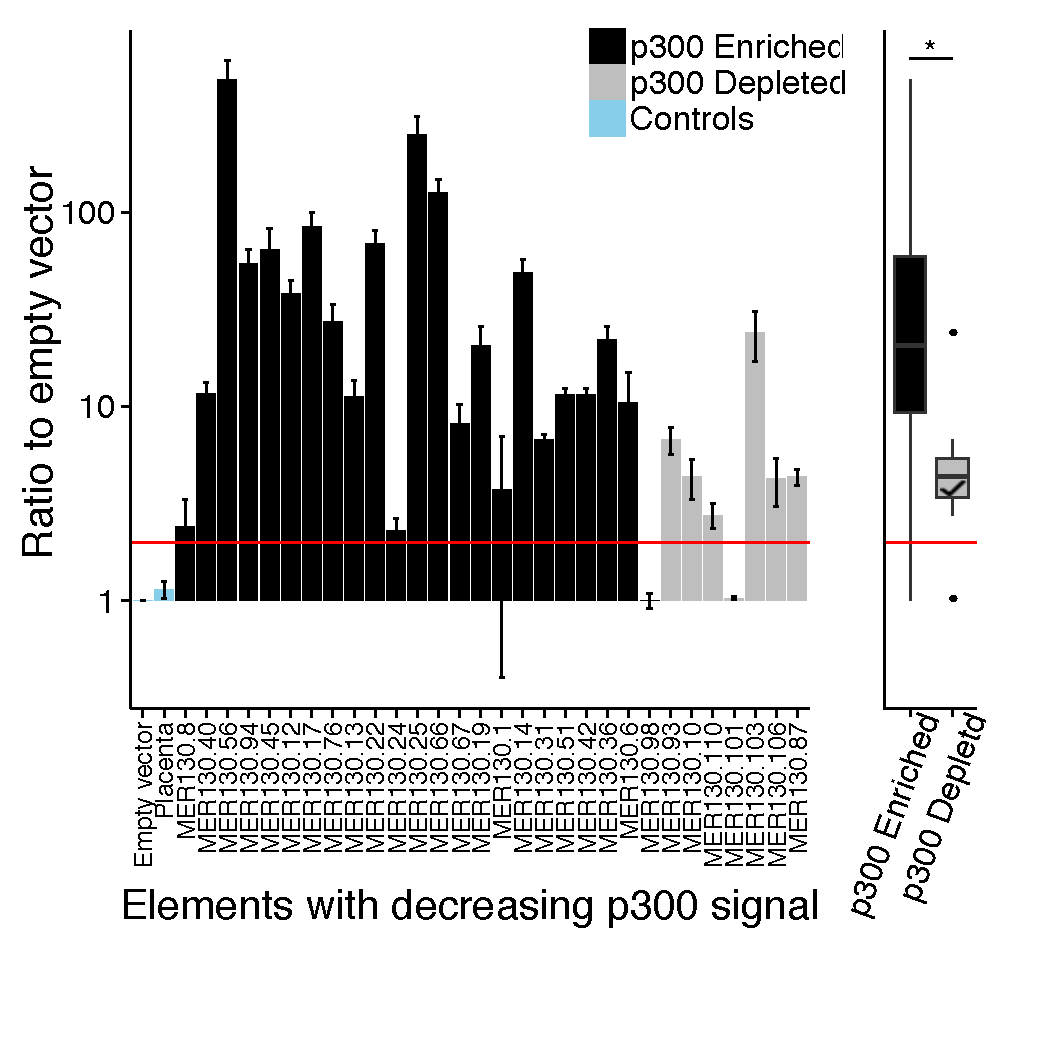
\epsfig{file=figures/mer130FigureS1.pdf,width=0.7\linewidth,clip=,trim=0 0 0 0} \\
\end{tabular}
\caption[MER130 instances function as enhancers in dissociated cortical neurons]{
{\bf MER130 instances function as enhancers in dissociated cortical neurons.}
Average fold activity when transfected
in dissociated cortical neurons relative to the empty vector. MER130
elements sorted in order of decreasing maximum p300 ChIP-seq intensity.
MER130 elements enriched for the p300 signal in black (\emph{n} = 23)
and depleted for the p300 signal in gray (\emph{n} = 7). Error bars
represent standard deviations. \emph{n} = 3 biological replicates x 3
technical replicates for each condition. t-test. *\emph{p}-value \textless{}
0.05.
}
\label{fig:mer130FigS1}
\end{figure}

\begin{figure}[htbp]
\centering
\begin{tabular}{l}

\epsfig{file=figures/mer130FigureS2.pdf,width=0.99\linewidth,clip=,trim=0 0 0 0} \\
\end{tabular}
\caption[MER130 multiple alignment]{
{\bf MER130 multiple alignment.}
A multiple alignment of all 107 MER130
instances, virtually all of which preserve the 5 binding site core.
}
\label{fig:mer130FigS2}
\end{figure}

\begin{figure}[htbp]
\centering
\begin{tabular}{l}
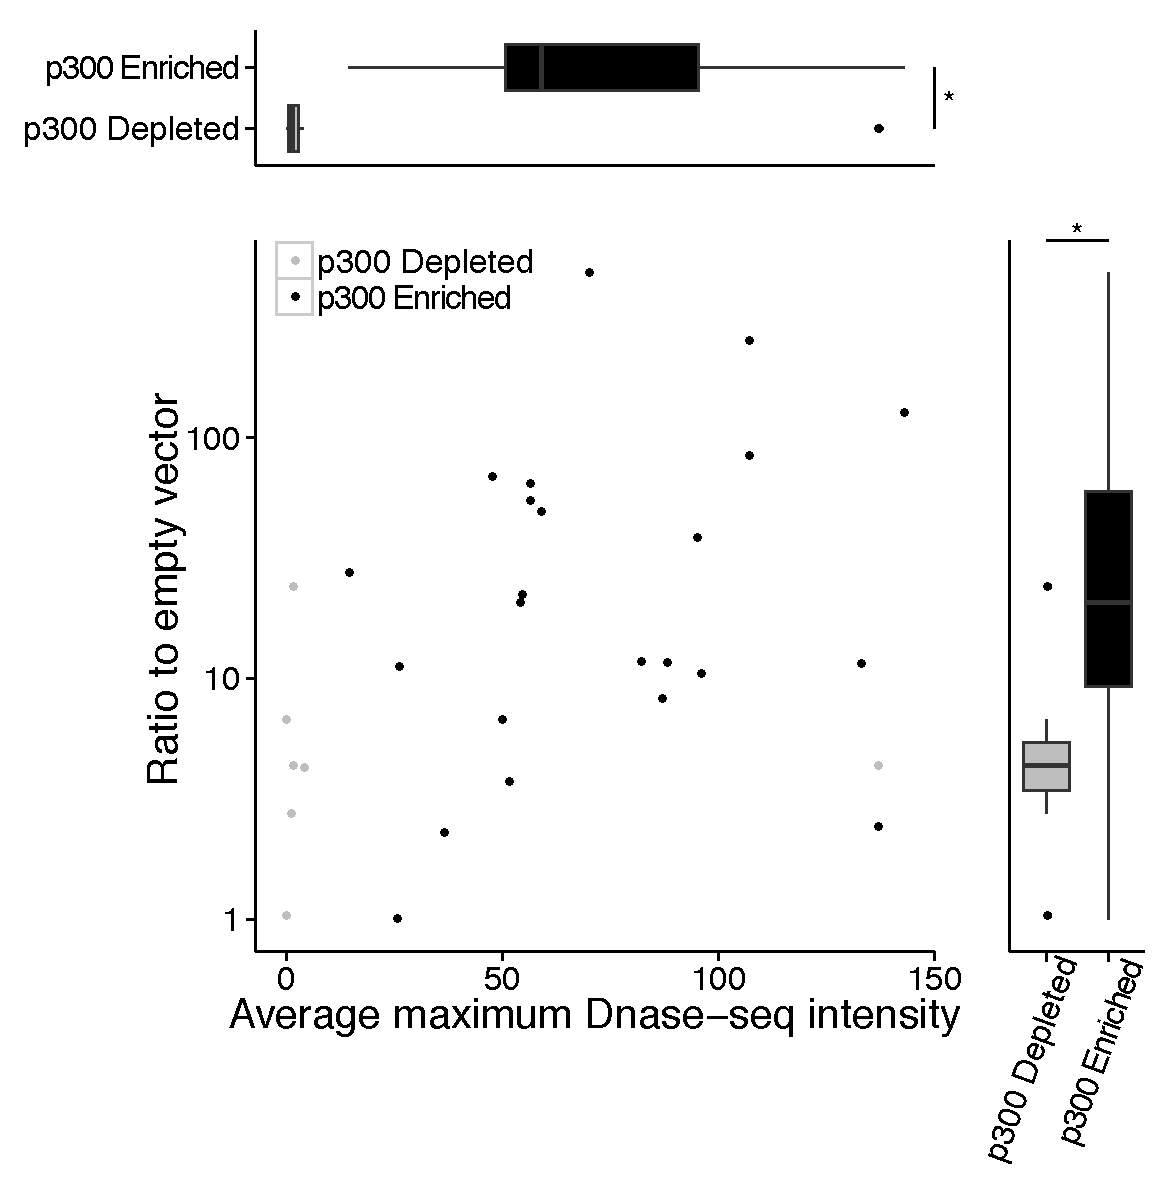
\epsfig{file=figures/mer130FigureS3.pdf,width=0.7\linewidth,clip=,trim=0 0 0 0} \\
\end{tabular}
\caption[DNase-seq intensity vs. transfection activity]{
{\bf DNase-seq intensity vs. transfection activity.}
Average DNase-seq intensity across day
85 human fetal brain tissue replicates (x-axis) plotted against average
fold activity relative to the empty vector (y-axis) for the same set of
MER130 instances transfected into dissociated cortical neurons. MER130
elements enriched for the p300 signal in black (\emph{n} = 23) and
depleted for the p300 signal in gray (\emph{n =} 7). t-test. *\emph{p}-value
\textless{} 0.05.
}
\label{fig:mer130FigS3}
\end{figure}

\section{Supplemental Tables}

\begin{center}
\begin{longtable}{@{}p{0.25\linewidth}p{0.2\linewidth}p{0.2\linewidth}p{0.2\linewidth}@{}}
\caption[MER130 instances in mouse]{{\bf MER130 instances in mouse.}
Identified by nhmmer (see Methods in \ref{sec:mer130Methods}) in the NCBI37/mm9 mouse assembly.
}
\label{tab:mer130TabS1} \\

\hline \textbf{mm9 chromosome} & \textbf{Start position} & \textbf{End position} & \textbf{Name} \\ \hline 
\endfirsthead

\hline \textbf{mm9 chromosome} & \textbf{Start position} & \textbf{End
position} & \textbf{Name} \\ \hline 
\endhead

\hline
\endlastfoot

chr3 & 149213528 & 149213837 & MER130.1\tabularnewline
chr15 & 42592816 & 42592880 & MER130.2\tabularnewline
chr1 & 192390632 & 192390976 & MER130.3\tabularnewline
chr10 & 111373706 & 111374076 & MER130.4\tabularnewline
chr12 & 93273917 & 93274100 & MER130.5\tabularnewline
chr16 & 82661316 & 82661607 & MER130.6\tabularnewline
chr5 & 59366593 & 59366899 & MER130.7\tabularnewline
chr10 & 91182667 & 91183115 & MER130.8\tabularnewline
chr2 & 6960107 & 6960257 & MER130.9\tabularnewline
chr5 & 76389906 & 76390041 & MER130.10\tabularnewline
chrX & 66281974 & 66282187 & MER130.11\tabularnewline
chr14 & 123357211 & 123357465 & MER130.12\tabularnewline
chr16 & 72088406 & 72088618 & MER130.13\tabularnewline
chr11 & 26486760 & 26487197 & MER130.14\tabularnewline
chr17 & 78850810 & 78851192 & MER130.15\tabularnewline
chr4 & 21475030 & 21475324 & MER130.16\tabularnewline
chr2 & 73770833 & 73771101 & MER130.17\tabularnewline
chr16 & 72585559 & 72585799 & MER130.18\tabularnewline
chr15 & 31919395 & 31919637 & MER130.19\tabularnewline
chr3 & 85197458 & 85197660 & MER130.20\tabularnewline
chr6 & 5906456 & 5906821 & MER130.21\tabularnewline
chr1 & 32520019 & 32520321 & MER130.22\tabularnewline
chr10 & 121383312 & 121383550 & MER130.23\tabularnewline
chr6 & 16907063 & 16907326 & MER130.24\tabularnewline
chr12 & 107258342 & 107258648 & MER130.25\tabularnewline
chr8 & 52773395 & 52773689 & MER130.26\tabularnewline
chr8 & 17465577 & 17465815 & MER130.27\tabularnewline
chr2 & 63948029 & 63948206 & MER130.28\tabularnewline
chr19 & 49153411 & 49153517 & MER130.29\tabularnewline
chr19 & 51802258 & 51802437 & MER130.30\tabularnewline
chr13 & 48123239 & 48123471 & MER130.31\tabularnewline
chr2 & 82213354 & 82213558 & MER130.32\tabularnewline
chr8 & 90169311 & 90169558 & MER130.33\tabularnewline
chr2 & 78185663 & 78185879 & MER130.34\tabularnewline
chr18 & 64598088 & 64598213 & MER130.35\tabularnewline
chr2 & 57759274 & 57759618 & MER130.36\tabularnewline
chr17 & 78303759 & 78304034 & MER130.37\tabularnewline
chr3 & 68157491 & 68157731 & MER130.38\tabularnewline
chr9 & 74166728 & 74166824 & MER130.39\tabularnewline
chr8 & 90199467 & 90199632 & MER130.40\tabularnewline
chr4 & 94106030 & 94106148 & MER130.41\tabularnewline
chr2 & 43672783 & 43673121 & MER130.42\tabularnewline
chr2 & 56085573 & 56085764 & MER130.43\tabularnewline
chr16 & 28761888 & 28761997 & MER130.44\tabularnewline
chr2 & 18556785 & 18556976 & MER130.45\tabularnewline
chr1 & 183952006 & 183952301 & MER130.47\tabularnewline
chr15 & 40900331 & 40900526 & MER130.48\tabularnewline
chr1 & 78050307 & 78050636 & MER130.49\tabularnewline
chr12 & 47472759 & 47473058 & MER130.50\tabularnewline
chr12 & 39028085 & 39028340 & MER130.51\tabularnewline
chr12 & 50030097 & 50030315 & MER130.52\tabularnewline
chr11 & 18387979 & 18388084 & MER130.53\tabularnewline
chr18 & 23505773 & 23505886 & MER130.54\tabularnewline
chr5 & 60668031 & 60668304 & MER130.55\tabularnewline
chr13 & 95145888 & 95146198 & MER130.56\tabularnewline
chr12 & 54713097 & 54713392 & MER130.57\tabularnewline
chr1 & 139743927 & 139744144 & MER130.58\tabularnewline
chr10 & 54469112 & 54469302 & MER130.59\tabularnewline
chr17 & 11669081 & 11669223 & MER130.60\tabularnewline
chrX & 143163220 & 143163378 & MER130.61\tabularnewline
chr11 & 19162882 & 19163203 & MER130.62\tabularnewline
chr4 & 99232256 & 99232380 & MER130.63\tabularnewline
chr6 & 111689190 & 111689279 & MER130.64\tabularnewline
chr7 & 140680006 & 140680246 & MER130.65\tabularnewline
chr2 & 50510542 & 50510637 & MER130.66\tabularnewline
chr6 & 100077946 & 100078114 & MER130.67\tabularnewline
chr6 & 19165247 & 19165397 & MER130.68\tabularnewline
chr12 & 27803589 & 27803695 & MER130.69\tabularnewline
chr6 & 6743998 & 6744232 & MER130.70\tabularnewline
chr7 & 58670946 & 58671173 & MER130.71\tabularnewline
chr1 & 48333229 & 48333326 & MER130.72\tabularnewline
chr15 & 35198547 & 35198786 & MER130.73\tabularnewline
chr4 & 82591594 & 82591793 & MER130.74\tabularnewline
chr7 & 36518733 & 36518948 & MER130.76\tabularnewline
chr15 & 22656438 & 22656591 & MER130.77\tabularnewline
chr9 & 47115318 & 47115455 & MER130.78\tabularnewline
chr7 & 72250084 & 72250179 & MER130.79\tabularnewline
chr9 & 105425505 & 105425645 & MER130.80\tabularnewline
chr12 & 39764820 & 39764975 & MER130.81\tabularnewline
chr10 & 116036701 & 116036794 & MER130.82\tabularnewline
chr12 & 37018024 & 37018167 & MER130.83\tabularnewline
chr8 & 54933223 & 54933464 & MER130.84\tabularnewline
chr1 & 148548001 & 148548049 & MER130.85\tabularnewline
chr9 & 30232922 & 30233018 & MER130.86\tabularnewline
chr16 & 83768718 & 83768845 & MER130.87\tabularnewline
chr5 & 106422248 & 106422376 & MER130.88\tabularnewline
chr12 & 12627126 & 12627374 & MER130.89\tabularnewline
chr18 & 17545739 & 17545816 & MER130.90\tabularnewline
chr10 & 51513821 & 51513991 & MER130.91\tabularnewline
chr4 & 82509395 & 82509591 & MER130.92\tabularnewline
chr6 & 19565949 & 19566025 & MER130.93\tabularnewline
chr11 & 91288193 & 91288316 & MER130.94\tabularnewline
chrX & 89586430 & 89586499 & MER130.95\tabularnewline
chr6 & 19845744 & 19845848 & MER130.96\tabularnewline
chr6 & 33048942 & 33049049 & MER130.97\tabularnewline
chr8 & 92938136 & 92938253 & MER130.98\tabularnewline
chr9 & 70057275 & 70057401 & MER130.99\tabularnewline
chr10 & 63593293 & 63593541 & MER130.100\tabularnewline
chr11 & 83419419 & 83419565 & MER130.101\tabularnewline
chr15 & 63001904 & 63002059 & MER130.102\tabularnewline
chr13 & 56044847 & 56045004 & MER130.103\tabularnewline
chr4 & 62294274 & 62294379 & MER130.105\tabularnewline
chr7 & 38134116 & 38134266 & MER130.106\tabularnewline
chr14 & 84434751 & 84434844 & MER130.107\tabularnewline
chr10 & 114109092 & 114109219 & MER130.109\tabularnewline
chr10 & 18152254 & 18152359 & MER130.110\tabularnewline
chr8 & 6533117 & 6533211 & MER130.112\tabularnewline
\end{longtable}
\end{center}

\begin{center}
\begin{longtable}{@{}p{0.17\linewidth}p{0.12\linewidth}p{0.15\linewidth}p{0.2\linewidth}p{0.2\linewidth}@{}}
\caption[Repeat densities observed in 75 vertebrate genome drafts from UCSC and Genbank]{{\bf Repeat densities observed in 75 vertebrate genome drafts from UCSC and Genbank.}
Repeat occurrences and repeat density observed in each vertebrate genome
}
\label{tab:mer130TabS2} \\

\hline \textbf{Common name} & \textbf{Genome assembly} & \textbf{MER130 instances} & \textbf{Genome or scaffold size} & \textbf{Repeat density (copies / Mb)} \\ \hline 
\endfirsthead

\hline \textbf{Common name} & \textbf{Genome assembly} & \textbf{MER130 instances} & \textbf{Genome or scaffold size} & \textbf{Repeat density (copies / Mb)} \\ \hline 
\endhead

\hline
\endlastfoot

Green sea turtle & Scaffold & 1124 & 2,208,393,880 &
0.508967178\tabularnewline
Painted turtle & chrPic1 & 1067 & 2,589,745,704 &
0.412009565\tabularnewline
Rock dove & Scaffold & 359 & 1,107,971,856 & 0.32401545\tabularnewline
Spiny softshell turtle & Scaffold & 621 & 1,931,078,847 &
0.321581898\tabularnewline
Saker falcon & Scaffold & 377 & 1,174,811,715 &
0.320902486\tabularnewline
Peregrine falcon & Scaffold & 375 & 1,171,955,363 &
0.319978057\tabularnewline
Duck & Scaffold & 340 & 1,105,035,747 & 0.307682354\tabularnewline
Budgerigar & melUnd1 & 331 & 1,117,373,619 & 0.296230369\tabularnewline
Chicken & galGal4 & 297 & 1,046,932,099 & 0.28368602\tabularnewline
American alligator & allMis1 & 616 & 2,174,259,888 &
0.283314798\tabularnewline
Scarlet macaw & Scaffold & 334 & 1,204,683,257 &
0.277251301\tabularnewline
Chinese soft shelled turtle & Scaffold & 608 & 2,202,466,388 &
0.276054156\tabularnewline
Turkey & melGal1 & 283 & 1,061,817,101 & 0.266524244\tabularnewline
Medium Ground Finch & geoFor1 & 283 & 1,065,292,181 &
0.265654818\tabularnewline
Medium ground finch & Scaffold & 283 & 1,065,292,181 &
0.265654818\tabularnewline
Ground tit & Scaffold & 277 & 1,042,980,823 & 0.265584941\tabularnewline
Zebra Finch & taeGut1 & 319 & 1,233,186,341 & 0.258679479\tabularnewline
White-throated sparrow & Scaffold & 267 & 1,052,600,561 &
0.253657475\tabularnewline
Platypus & ornAna1 & 224 & 1,996,811,212 & 0.112178857\tabularnewline
Lizard & anoCar2 & 141 & 1,799,143,587 & 0.078370621\tabularnewline
White rhinoceros & cerSim1 & 192 & 2,464,367,180 &
0.077910468\tabularnewline
Horse & equCab2 & 191 & 2,484,532,062 & 0.076875643\tabularnewline
Panda & ailMel1 & 168 & 2,299,509,015 & 0.073059074\tabularnewline
Alpaca & vicPac2 & 158 & 2,172,177,994 & 0.072738054\tabularnewline
Megabat & pteVam1 & 140 & 1,996,076,410 & 0.070137596\tabularnewline
Microbat & myoLuc2 & 141 & 2,034,575,300 & 0.069301932\tabularnewline
Cat & felCat5 & 169 & 2,455,541,136 & 0.068823934\tabularnewline
Dog & canFam3 & 164 & 2,410,976,875 & 0.06802222\tabularnewline
Bushbaby & otoGar3 & 167 & 2,519,724,550 & 0.066277086\tabularnewline
Tasmanian devil & sarHar1 & 206 & 3,174,693,010 &
0.064888164\tabularnewline
Opossum & monDom5 & 232 & 3,605,631,728 & 0.064343787\tabularnewline
Ferret & musFur1 & 155 & 2,410,758,013 & 0.06429513\tabularnewline
Dolphin & turTru2 & 164 & 2,551,996,573 & 0.064263409\tabularnewline
Squirrel monkey & saiBol1 & 166 & 2,608,572,064 &
0.063636348\tabularnewline
Squirrel & speTri2 & 155 & 2,478,393,770 & 0.062540506\tabularnewline
Manatee & triMan1 & 191 & 3,103,808,406 & 0.061537304\tabularnewline
Baboon & papAnu2 & 178 & 2,948,380,710 & 0.060372122\tabularnewline
Rhesus & rheMac3 & 179 & 2,969,988,180 & 0.0602696\tabularnewline
Gibbon & nomLeu3 & 176 & 2,962,077,449 & 0.059417758\tabularnewline
Marmoset & calJac3 & 172 & 2,914,958,544 & 0.059005985\tabularnewline
Sheep & oviAri3 & 153 & 2,619,054,388 & 0.058418031\tabularnewline
Pig & susScr3 & 164 & 2,808,525,991 & 0.05839362\tabularnewline
Gorilla & gorGor3 & 175 & 3,029,553,646 & 0.057764285\tabularnewline
Elephant & loxAfr3 & 183 & 3,196,760,833 & 0.057245446\tabularnewline
Wallaby & macEug2 & 174 & 3,075,184,024 & 0.05658198\tabularnewline
Human & hg19 & 176 & 3,137,161,264 & 0.056101674\tabularnewline
Orangutan & ponAbe2 & 189 & 3,446,771,396 & 0.054833924\tabularnewline
Chimpanzee & panTro4 & 177 & 3,309,577,922 & 0.05348114\tabularnewline
Sloth & choHof1 & 131 & 2,458,927,620 & 0.053275257\tabularnewline
Cow & bosTau7 & 155 & 2,981,119,579 & 0.051993889\tabularnewline
Kangaroo rat & dipOrd1 & 112 & 2,158,502,098 &
0.051887835\tabularnewline
Rabbit & oryCun2 & 140 & 2,737,490,501 & 0.05114173\tabularnewline
Naked mole-rat & hetGla2 & 128 & 2,618,204,639 &
0.048888463\tabularnewline
Mouse lemur & micMur1 & 140 & 2,902,270,736 & 0.048238091\tabularnewline
Tarsier & tarSyr1 & 152 & 3,179,905,132 & 0.047800168\tabularnewline
Guinea Pig & cavPor3 & 128 & 2,723,219,641 & 0.047003186\tabularnewline
Tenrec & echTel2 & 132 & 2,947,024,286 & 0.044790944\tabularnewline
Rock hyrax & proCap1 & 128 & 2,985,258,999 & 0.042877352\tabularnewline
Armadillo & dasNov3 & 155 & 3,631,522,711 & 0.04268182\tabularnewline
Mouse & mm9 & 113 & 2,725,765,481 & 0.041456244\tabularnewline
Rat & rn5 & 114 & 2,909,698,938 & 0.039179311\tabularnewline
Frog (X. tropicalis) & xenTro3 & 55 & 1,511,735,326 &
0.03638203\tabularnewline
Tree shrew & tupBel1 & 117 & 3,660,774,957 & 0.031960446\tabularnewline
Shrew & sorAra1 & 93 & 2,936,119,008 & 0.031674465\tabularnewline
Pika & ochPri2 & 105 & 3,445,784,354 & 0.030472017\tabularnewline
Hedgehog & eriEur1 & 97 & 3,367,787,358 & 0.028802294\tabularnewline
Coelacanth & latCha1 & 1 & 2,860,591,921 & 0.000349578\tabularnewline
Zebrafish & danRer7 & 0 & 1,412,464,843 & 0\tabularnewline
Fugu & fr3 & 0 & 391,484,715 & 0\tabularnewline
Atlantic cod & gadMor1 & 0 & 824,327,835 & 0\tabularnewline
Stickleback & gasAcu1 & 0 & 463,354,448 & 0\tabularnewline
Nile tilapia & oreNil2 & 0 & 927,696,114 & 0\tabularnewline
Medaka & oryLat2 & 0 & 869,000,216 & 0\tabularnewline
Lamprey & petMar2 & 0 & 885,550,958 & 0\tabularnewline
Tetraodon & tetNig2 & 0 & 358,618,246 & 0\tabularnewline
\end{longtable}
\end{center}

\begin{landscape}
\begin{center}
\begin{longtable}
{@{}>{\hspace{0pt}}p{0.2\linewidth}>{\hspace{0pt}}p{0.4\linewidth}>{\hspace{0pt}}p{0.4\linewidth}@{}}
\caption[MER130 PCR primers]{{\bf MER130 PCR primers.}
PCR primers used
to clone candidate enhancer elements.
}
\label{tab:mer130TabS3} \\

\hline \textbf{Name} & \textbf{Forward} & \textbf{Reverse} \\ \hline 
\endfirsthead

\hline \textbf{Name} & \textbf{Forward} & \textbf{Reverse} \\ \hline 
\endhead

\hline
\endlastfoot

MER130.10 & ggatggaggatcGTGTCGTACCCTGTTTTCTCA &
ggtaaggtggatcCACAGCCAGGCACGTACA\tabularnewline
MER130.101 & ggatggaggatcCTGGGTTGATTCTCCAGCA &
ggtaaggtggatcGCCTAGCACACCCCACA\tabularnewline
MER130.103 & ggatggaggatcTGGCACAAGAAAGAATAGGTG &
ggtaaggtggatcTGCCAGGGACTGCTTGA\tabularnewline
MER130.106 & ggatggaggatcCCTCCGAGCCCCAAAC &
ggtaaggtggatcGCGTCCCTCTGCTTCCT\tabularnewline
MER130.110 & ggatggaggatcTTAAGGTGGAAATGTTTGTTGA &
ggtaaggtggatcACAGCATGTTCTTTTACCCAAT\tabularnewline
MER130.13 & ggatggaggatcGGGGGAGATCGGAAGC &
ggtaaggtggatcGCGGTCGAAACCTTTGAA\tabularnewline
MER130.14 & ggatggaggatcCACCAATCCAGGGAAATGA &
ggtaaggtggatcGGACTTGCAGGGGAGTCA\tabularnewline
MER130.17 & ggatggaggatcTGAGGCAGATCCAGAGAGG &
ggtaaggtggatcAGCTGGGTCTTTCCCAGAG\tabularnewline
MER130.19 & ggatggaggatcGGGTCCTAGTGTGCAGCAG &
ggtaaggtggatcCGCCTTGGACCCCAAC\tabularnewline
MER130.22 & ggatggaggatcAACTCAGATTGTCTGCCTTGG &
ggtaaggtggatcAAGGTTGCATAACACAGTTTCA\tabularnewline
MER130.24 & ggatggaggatcGGCCCTCTAAAGCATCTGG &
ggtaaggtggatcGGCACTGGTGTCGAGAGTC\tabularnewline
MER130.31 & ggatggaggatcTCCTGACTTCGGGATTTAGA &
ggtaaggtggatcCAGAGCCGCCAGTGGT\tabularnewline
MER130.36 & ggatggaggatcCAAAGGTACTAGGTGGGAATTG &
ggtaaggtggatcCTTGATACATGGAATGAAACCA\tabularnewline
MER130.40 & ggatggaggatcCAGAGGGGCAGTGGAAGA &
ggtaaggtggatcCCCAGATCCCGATGACC\tabularnewline
MER130.42 & ggatggaggatcGGGGGAATTGTCCCCTTA &
ggtaaggtggatcTGAATGAATGGCTTCAGCA\tabularnewline
MER130.45 & ggatggaggatcGGTGCCCAGGTTCTGCT &
ggtaaggtggatcAAGGCAGGAGCTGACAGG\tabularnewline
MER130.51 & ggatggaggatcGATTTCTGGGGCATTTTGA &
ggtaaggtggatcTGGCTGTTTTAGGGGGAAT\tabularnewline
MER130.56 & ggatggaggatcGGTGATTATTCTCAGTGGCAGT &
ggtaaggtggatcGCTTCAGAGACGAGCTTATTGC\tabularnewline
MER130.6 & ggatggaggatcAAAAGTTTTGTGCTTTCCAACA &
ggtaaggtggatcTGCCACACTGAAGGACTCTAA\tabularnewline
MER130.66 & ggatggaggatcGGCACCTAAAAGATCGGAATC &
ggtaaggtggatcGCCGTTGTAAGCAGTTTTGA\tabularnewline
MER130.67 & ggatggaggatcGGGTCAGGTGCCAGGA &
ggtaaggtggatcCCAGACTCCTACAGGTCAGATT\tabularnewline
MER130.76 & ggatggaggatcTCGGGCTTCTGTTTCACC &
ggtaaggtggatcGGCACTCAGCTCAGGAACA\tabularnewline
MER130.8 & ggatggaggatcTGGCGCACACTTTTCTTTC &
ggtaaggtggatcTGGCTCCTTCCCACCA\tabularnewline
MER130.87 & ggatggaggatcCCAAAACTCTTTGTTCATTTGTC &
ggtaaggtggatcCAAGGCTGTCCACTCTTCCT\tabularnewline
MER130.93 & ggatggaggatcCGCTCTATCCTGCCCTCA &
ggtaaggtggatcCAGGCAAAACTCTGCATTGA\tabularnewline
MER130.94 & ggatggaggatcGCCACAAATGGTCCAGAAA &
ggtaaggtggatcTGGAAAGCTATGTGGGTTTG\tabularnewline
MER130.98 & ggatggaggatcGATTGGACTCCATGAAAAAGC &
ggtaaggtggatcTGCACAGGGCTCCACTT\tabularnewline
MER130.25 & ggatggaggatcCCTGTGCTCATGGCTCCT &
ggtaaggtggatcTCTGGCTAGAAGAAAGAGGAAA\tabularnewline
MER130.26 & ggatggaggatcAGCGAAGGGAAGAACTCCA &
ggtaaggtggatcGAGGCAAAGGGAAGAGGAA\tabularnewline
MER130.27 & ggatggaggatcTTGGAATCCTTGCCATCTTT &
ggtaaggtggatcTGTTCTAAGGGGAAAACAGAGA\tabularnewline
MER130.31 WT & ggatggaggatcGCAGCAAGGAAGGGAAAA &
ggtaaggtggatcTGCTCAGGAATGCAGCAG\tabularnewline
MER130.31 MUT 1 & GGGCTTCTTGTCTAAAGCCGGCCGGGCAGGCCTGGGTTTTGGCAAAGCCAGTC
& GACTGGCTTTGCCAAAACCCAGGCCTGCCCGGCCGGCTTTAGACAAGAAGCCC\tabularnewline
MER130.31 MUT 2 & GCCAGTCGACTCTCCTACGGCCGTTACGGCCGCCATGGTAACAGATGGCCAGG
& CCTGGCCATCTGTTACCATGGCGGCCGTAACGGCCGTAGGAGAGTCGACTGGC\tabularnewline
MER130.31 MUT 3 & CGACTCTCCTACAAGCTGGCACGGCCGACGCGGCCCAGATGGCCAGGAGCGTAG
& CTACGCTCCTGGCCATCTGGGCCGCGTCGGCCGTGCCAGCTTGTAGGAGAGTCG\tabularnewline
MER130.31 MUT 4 & CAAGCTGGCACAAGGCCATGGGGCCCTCGCGGCCGGAGCGTAGGCAGCAAGG &
CCTTGCTGCCTACGCTCCGGCCGCGAGGGCCCCATGGCCTTGTGCCAGCTTG\tabularnewline
MER130.31 MUT 5 & GTAACAGATGGCCAGGAGCGTAGGCCTACCCGGCCGCAAAGGAAAGCATGTAGG
& CCTACATGCTTTCCTTTGCGGCCGGGTAGGCCTACGCTCCTGGCCATCTGTTAC\tabularnewline
MER130.45 WT & ggatggaggatcGGTGCCCAGGTTCTGCT &
ggtaaggtggatcAAGGCAGGAGCTGACAGG\tabularnewline
MER130.45 MUT 1 & GTTGCTGGAGTAAACTGTTAGGCCGAGCCGGCCTACACACTGAGGCAGGAGTC
& GACTCCTGCCTCAGTGTGTAGGCCGGCTCGGCCTAACAGTTTACTCCAGCAAC\tabularnewline
MER130.45 MUT 2 & GAGGCAGGAGTCCAAACTTGAGGCCTTTACGGCCGCCATGTCAGCAGATGGGC
& GCCCATCTGCTGACATGGCGGCCGTAAAGGCCTCAAGTTTGGACTCCTGCCTC\tabularnewline
MER130.45 MUT 3 & GTCCAAACTTGTAGATGGGCAGGCCTAACGGGCCGCAGATGGGCACAGGGAAAG
& CTTTCCCTGTGCCCATCTGCGGCCCGTTAGGCCTGCCCATCTACAAGTTTGGAC\tabularnewline
MER130.45 MUT 4 & GATGGGCAGCCAGCCATGTCAGGCCCGTTCGGCCGGGAAAGCGGCCAAGGAAG
& CTTCCTTGGCCGCTTTCCCGGCCGAACGGGCCTGACATGGCTGGCTGCCCATC\tabularnewline
MER130.45 MUT 5 & CAGCAGATGGGCACAGGGAAGGCCTAACCGGCCGCATGTGTGTGCATCCAGC &
GCTGGATGCACACACATGCGGCCGGTTAGGCCTTCCCTGTGCCCATCTGCTG\tabularnewline
Coelacanth & ggatggaggatcGCACCCCTTGAAAATGGG &
ggtaaggtggatcGCAGACATAACGGCGTC\tabularnewline
\end{longtable}
\end{center}
\end{landscape}


    \chapter{Supplemental material for \chapref{chap:autism}}
\label{chap:autismSuppl}

\section{Supplemental Figures}

\begin{figure}[htbp]
\centering
\begin{tabular}{l}
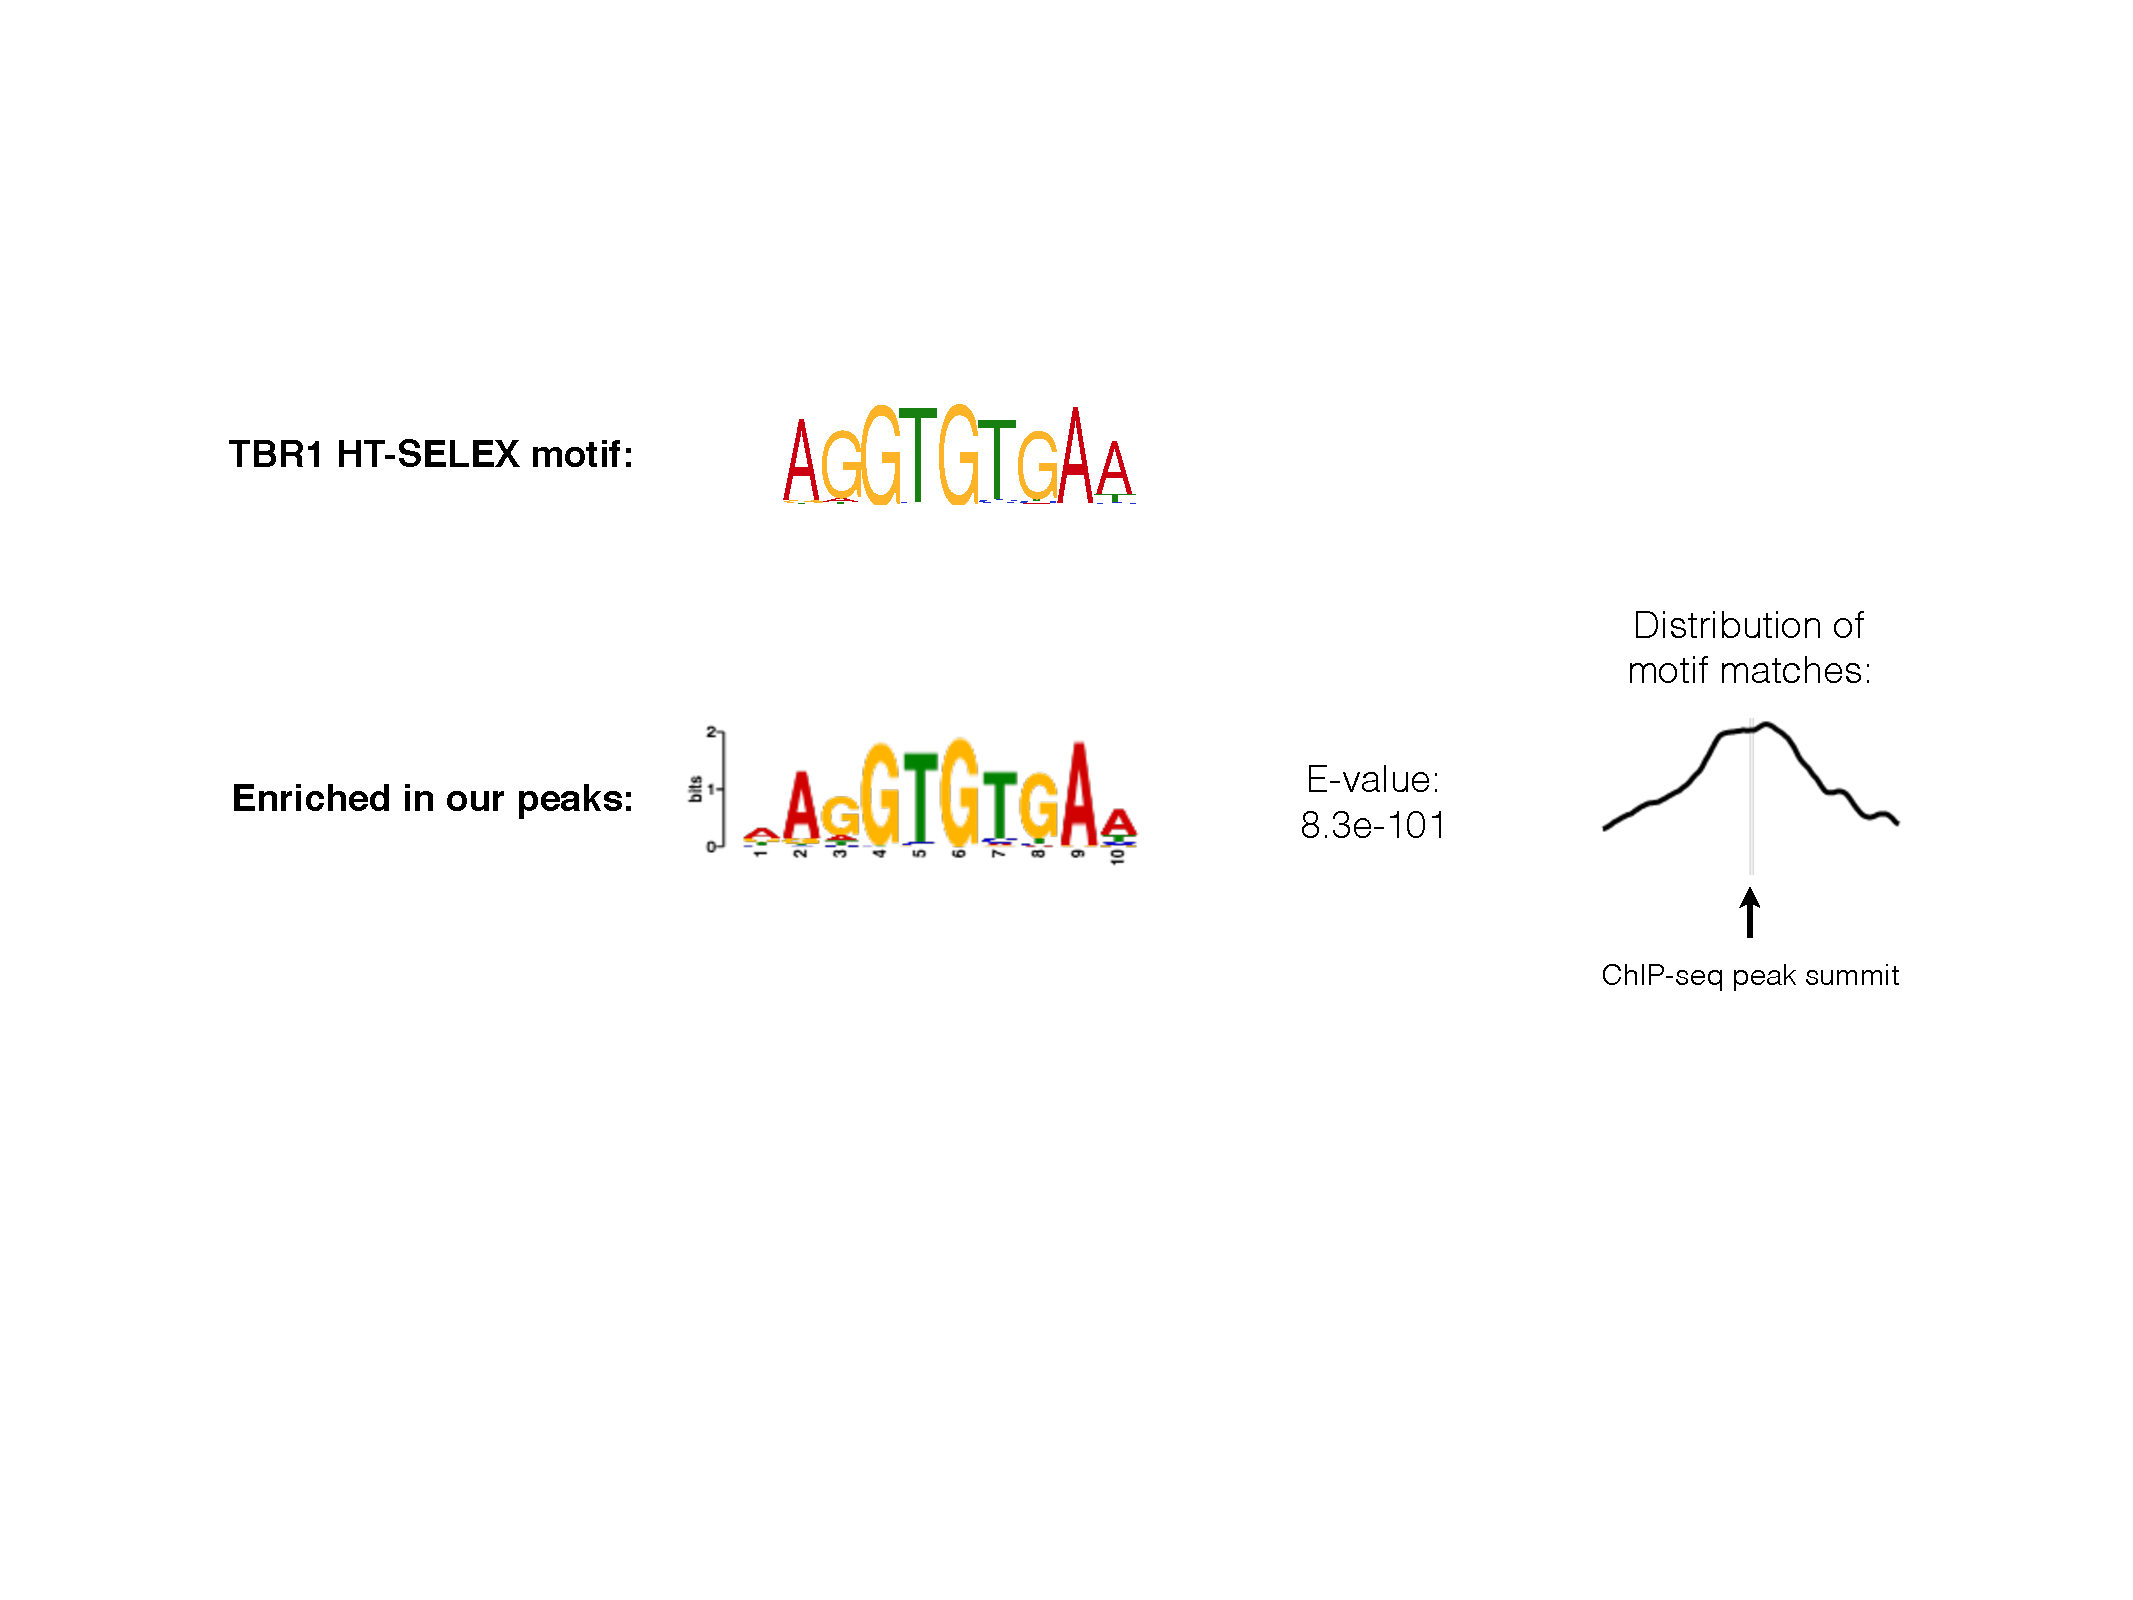
\epsfig{file=figures/autismFigureS1.pdf,width=0.99\linewidth,clip=,trim=0 0 0 0} \\
\end{tabular}
\caption[Motif discovery recovers TBR1 motif]{
{\bf Motif discovery recovers TBR1 motif.}
MEME-ChIP~\citep{Machanick:2011ge} motif discovery
recovers the known TBR1 motif~\citep{Jolma:2013fh} enriched at the
summits of ChIP-seq peaks.
}
\label{fig:autismFigS1}
\end{figure}

\begin{figure}[htbp]
\centering
\begin{tabular}{l}
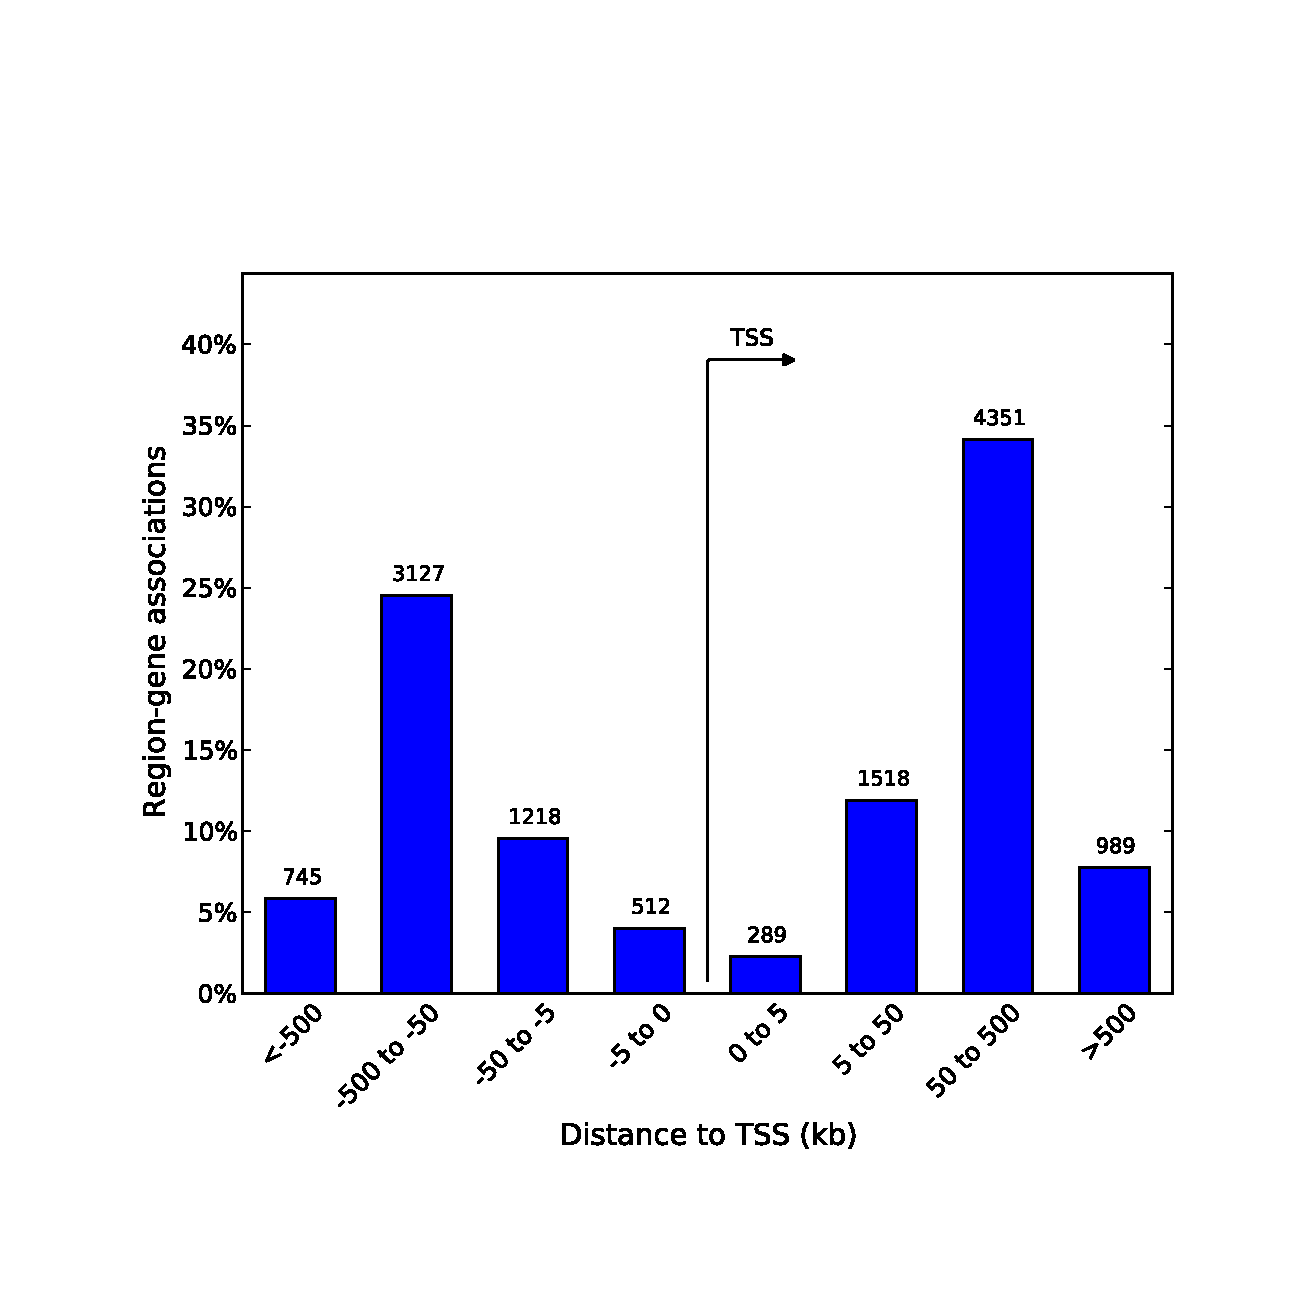
\epsfig{file=figures/autismFigureS2.pdf,width=0.8\linewidth,clip=,trim=0 0 0 0} \\
\end{tabular}
\caption[TBR1 peak distance to TSS distribution]{
{\bf TBR1 peak distance to TSS distribution.}
Distribution of TBR1 ChIP-seq peak distances to the
associated transcription start
sites.
}
\label{fig:autismFigS2}
\end{figure}

\begin{figure}[htbp]
\centering
\begin{tabular}{l}
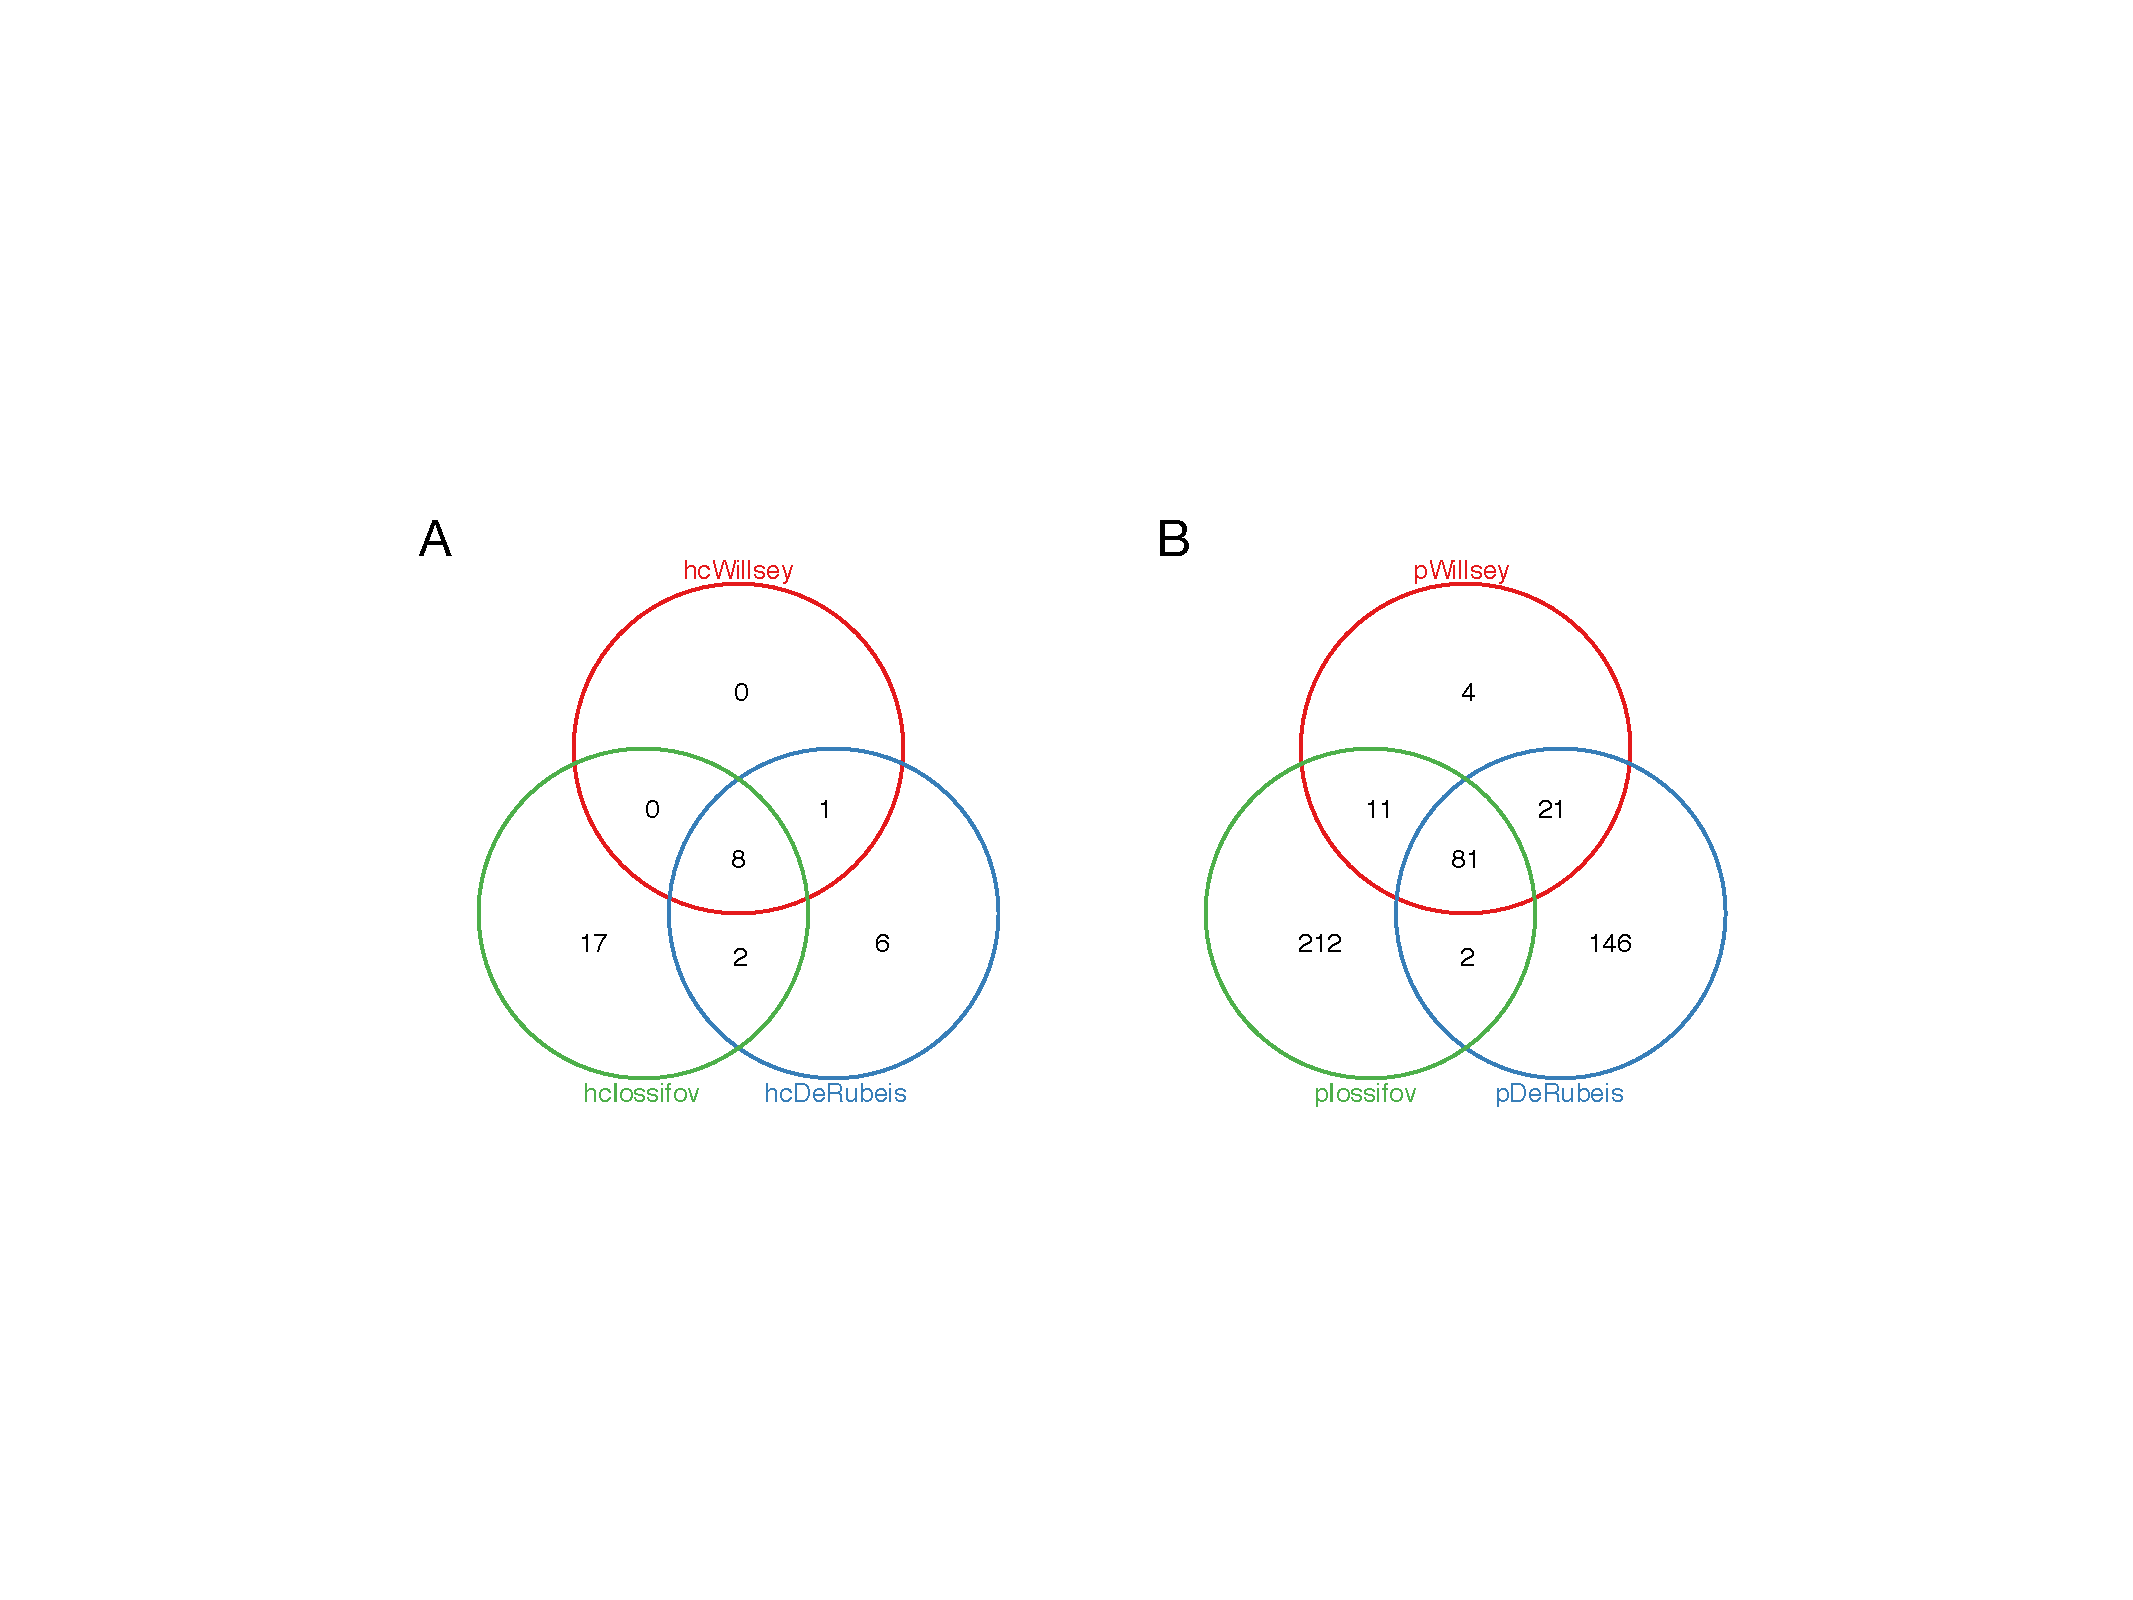
\epsfig{file=figures/autismFigureS3.pdf,width=0.99\linewidth,clip=,trim=0 0 0 0} \\
\end{tabular}
\caption[Autism risk gene overlap between studies]{
{\bf Autism risk gene overlap between studies.}
Overlaps among the mouse orthologs of high-confidence
{\bf (A)} and probable {\bf (B)} ASD genes from different studies. \emph{SYNGAP1}
was not mapped from the high-confidence human ASD gene set to mouse.
}
\label{fig:autismFigS3}
\end{figure}

\begin{figure}[htbp]
\centering
\begin{tabular}{l}
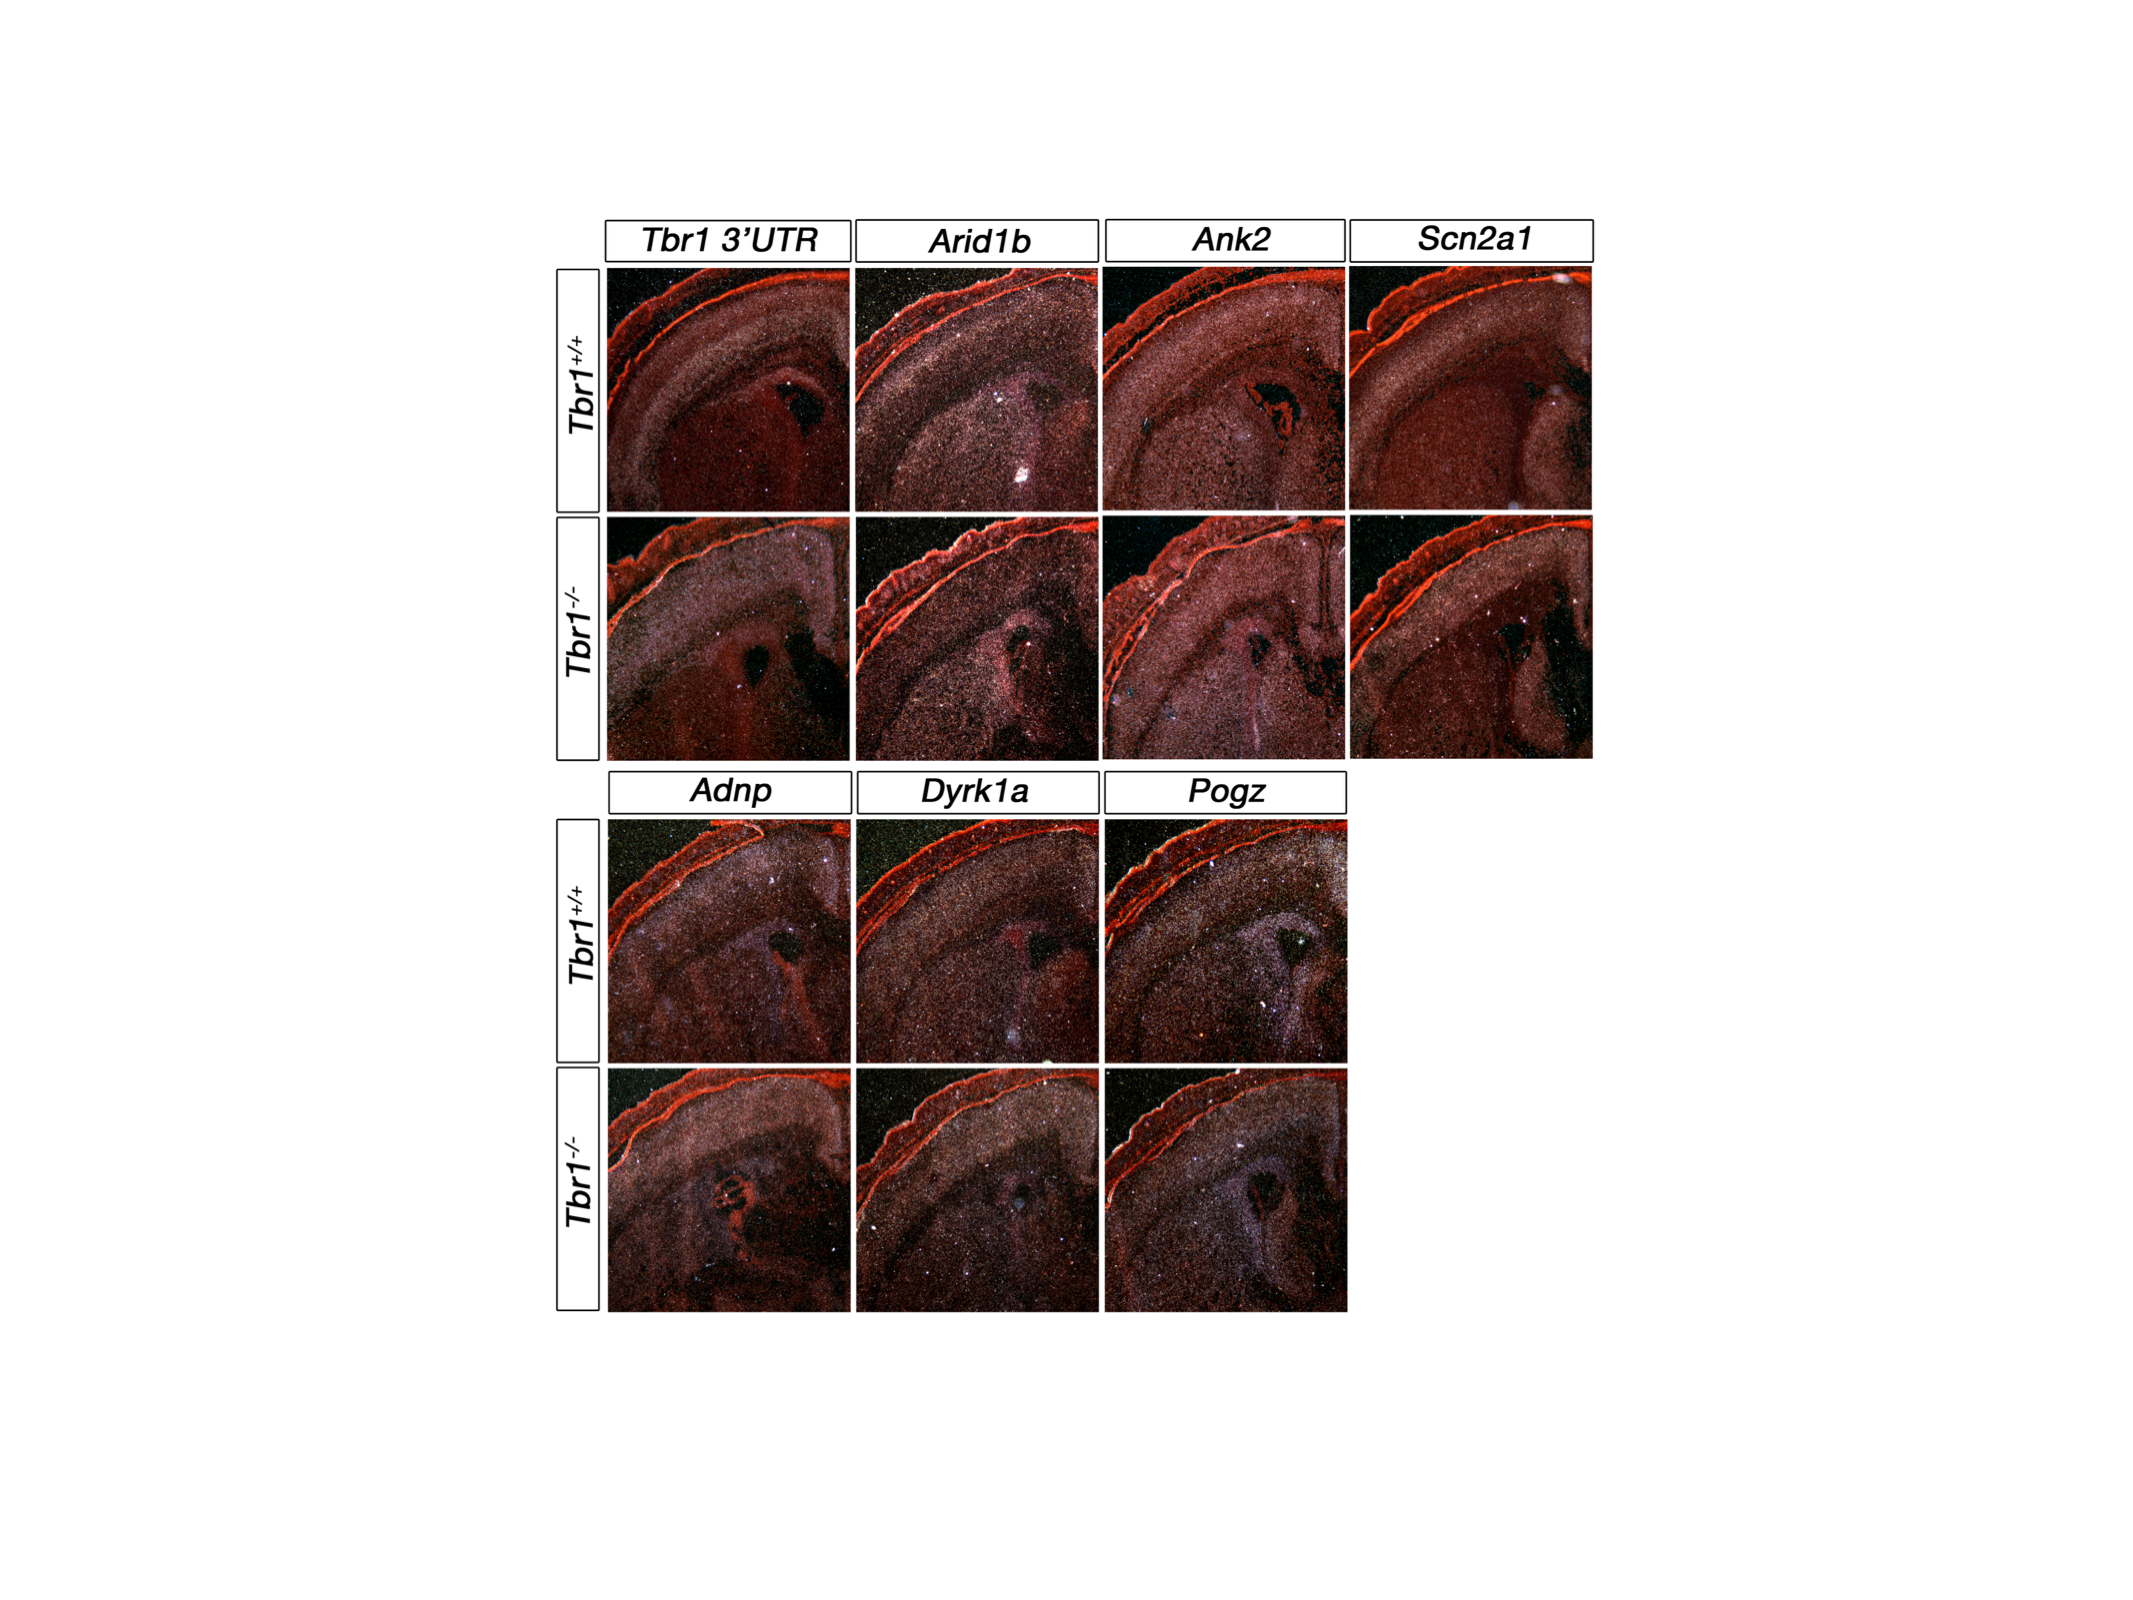
\epsfig{file=figures/autismFigureS4.pdf,width=0.99\linewidth,clip=,trim=0 0 0 0} \\
\end{tabular}
\caption[RISH \emph{in situs} of high-confidence ASD genes]{
{\bf RISH \emph{in situs} of high-confidence ASD genes.}
Radioactive \emph{in situ} hybridization (RISH) of
high-confidence ASD genes at P0 in \emph{Tbr1}\textsuperscript{+/+} and
\emph{Tbr1\textsuperscript{-/-}} cortices reveals expression
differences.
}
\label{fig:autismFigS4}
\end{figure}

\begin{figure}[htbp]
\centering
\begin{tabular}{l}
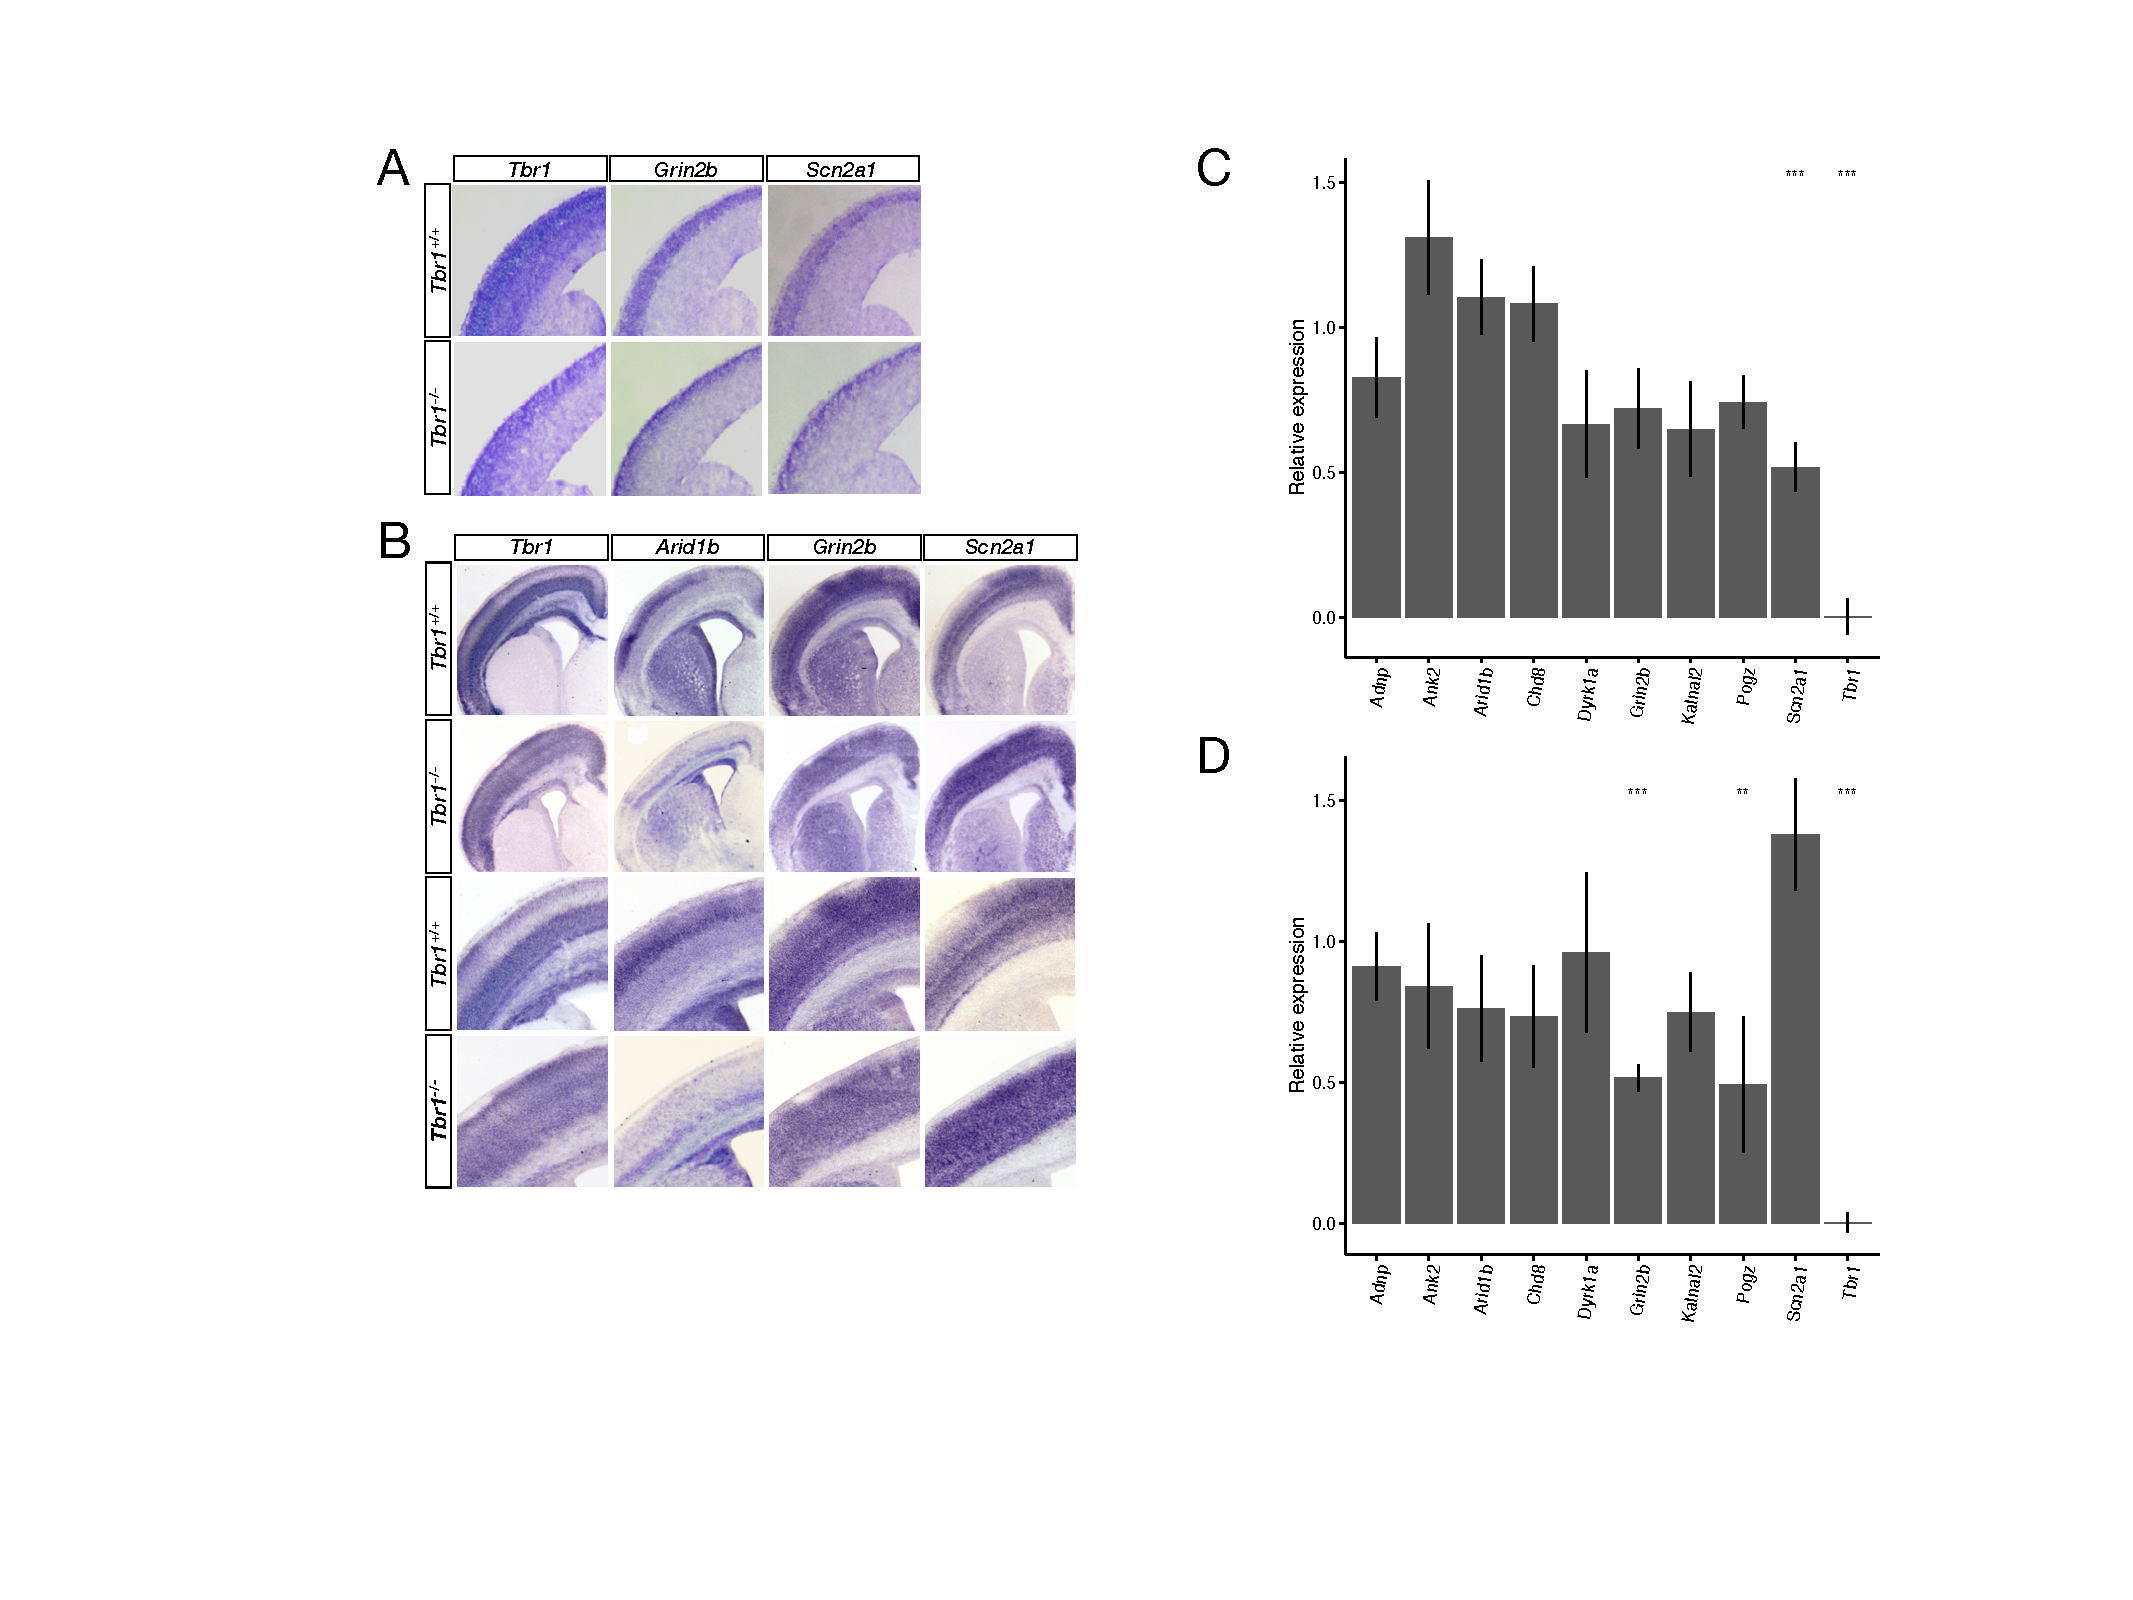
\epsfig{file=figures/autismFigureS5.pdf,width=0.99\linewidth,clip=,trim=0 0 0 0} \\
\end{tabular}
\caption[DIG \emph{in situs} of high-confidence ASD genes]{
{\bf DIG \emph{in situs} of high-confidence ASD genes.}
Digoxigenin (DIG) \emph{in situ} hybridization of
high-confidence genes at E14.5 {\bf (A)} and P0 {\bf (B)} in
\emph{Tbr1}\textsuperscript{+/+} and \emph{Tbr1\textsuperscript{-/-}}
cortices reveals expression differences. Relative expression corresponds
to quantitative real-time PCR (qRT-PCR) results comparing transcript
expression levels in the cortex of the \emph{Tbr1} mutant mice and
wild-type littermates at E14.5 {\bf (C)} and P0 {\bf (D)}. The error bars represent
the standard error of the mean. 2-sided \emph{t}-test. **\emph{p}-value
\textless{} 0.01; ***\emph{p}-value \textless{} 0.001.
}
\label{fig:autismFigS5}
\end{figure}

\begin{figure}[htbp]
\centering
\begin{tabular}{l}
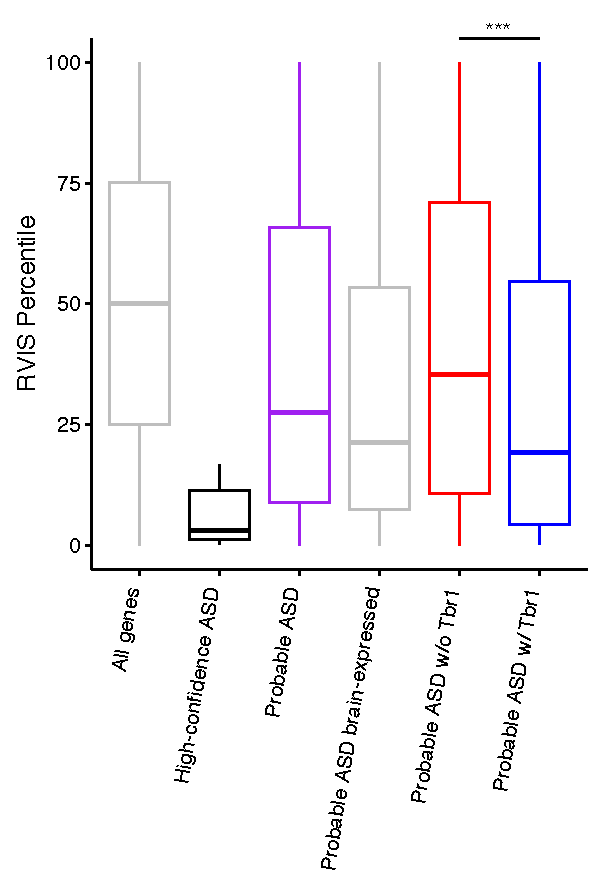
\epsfig{file=figures/autismFigureS6.pdf,width=0.6\linewidth,clip=,trim=0 0 0 0} \\
\end{tabular}
\caption[RVIS percentile distributions for ASD genes]{
{\bf RVIS percentile distributions for ASD genes.}
Probable ASD genes that are TBR1 targets are depleted
for RVIS percentiles. Box-plots depicting the distributions of RVIS
percentiles for different ASD gene lists (x-axis). Probable ASD genes
with adjacent TBR1 ChIP-seq peaks in the developing cortex (blue) have
lower RVIS percentiles than those without an adjacent TBR1 peak (red).
Significance was determined using the 1-sided 2-sample Wilcoxon test.
***\emph{p}-value \textless{} 0.001.
}
\label{fig:autismFigS6}
\end{figure}

\section{Supplemental Tables}

\begin{landscape}
\begin{center}
\begin{longtable}{@{}>{\hspace{0pt}}p{0.08\linewidth}>{\hspace{0pt}}p{0.08\linewidth}>{\hspace{0pt}}p{0.1\linewidth}>{\hspace{0pt}}p{0.17\linewidth}>{\hspace{0pt}}p{0.05\linewidth}>{\hspace{0pt}}p{0.06\linewidth}>{\hspace{0pt}}p{0.07\linewidth}>{\hspace{0pt}}p{0.05\linewidth}>{\hspace{0pt}}p{0.06\linewidth}>{\hspace{0pt}}p{0.06\linewidth}>{\hspace{0pt}}p{0.07\linewidth}@{}}
\caption[Autism risk gene metrics]{{\bf Autism risk gene metrics.}
The number of TBR1 ChIP-seq peaks adjacent to the
mouse ortholog, GREAT bionmial \emph{p-}value, fraction LoF score,
fraction LoF percentile among all genes, Icelandic knockout status, and
limma \emph{p}-value and fold for each high-confidence and probable ASD
gene. ``NA'' describes missing values.
}
\label{tab:autismTabS1} \\

\hline \textbf{Gene symbol} & \textbf{Merged gene list} & \textbf{Gene lists} & \textbf{Ensembl Identifier} & \textbf{\#
Tbr1 peaks} & \textbf{\# Tbr1 peaks GREAT binomial \emph{p}-value} & \textbf{Fraction LoF}
& \textbf{Fraction LoF percentile} & \textbf{Icelandic KO status} & \textbf{limma E14.5
log(fold-change)} & \textbf{limma E14.5 \emph{p}-value} \\ \hline 
\endfirsthead

\hline \textbf{Gene symbol} & \textbf{Merged gene list} & \textbf{Gene lists} & \textbf{Ensembl Identifier} & \textbf{\#
Tbr1 peaks} & \textbf{\# Tbr1 peaks GREAT binomial \emph{p}-value} & \textbf{Fraction LoF}
& \textbf{Fraction LoF percentile} & \textbf{Icelandic KO status} & \textbf{limma E14.5
log(fold-change)} & \textbf{limma E14.5 \emph{p}-value} \\ \hline 
\endhead

\hline
\endlastfoot

\emph{NFIB} & probable & pIossifov & ENSG00000147862 & 14 & 5.44E-05 &
3.31E-06 & 0.30 & Normal & 1.55 & 4.23E-03\tabularnewline
\emph{PBX1} & probable & pDeRubeis & ENSG00000185630 & 12 & 5.32E-03 &
1.64E-05 & 0.33 & Normal & 0.86 & 2.72E-02\tabularnewline
\emph{NFIA} & probable & pIossifov, pDeRubeis, pWillsey &
ENSG00000162599 & 12 & 4.05E-05 & 4.85E-05 & 0.41 & Normal & 1.26 &
9.09E-03\tabularnewline
\emph{ZFHX3} & probable & pIossifov & ENSG00000140836 & 12 & 6.12E-03 &
1.27E-04 & 0.54 & Normal & -0.44 & 8.92E-02\tabularnewline
\emph{MYT1L} & probable & pDeRubeis & ENSG00000186487 & 10 & 2.54E-03 &
9.87E-06 & 0.31 & Normal & 0.94 & 2.56E-02\tabularnewline
\emph{DSCAM} & high-confidence & hcIossifov, pDeRubeis & ENSG00000171587
& 10 & 3.58E-04 & 2.50E-05 & 0.36 & Normal & 0.39 &
3.29E-01\tabularnewline
\emph{INSC} & probable & pDeRubeis & ENSG00000188487 & 9 & 3.31E-03 &
3.21E-04 & 0.68 & Normal & -0.02 & 8.64E-01\tabularnewline
\emph{ELAVL2} & probable & pIossifov & ENSG00000107105 & 8 & 1.42E-01 &
3.63E-05 & 0.38 & Normal & 1.85 & 3.71E-02\tabularnewline
\emph{PARD3B} & probable & pIossifov & ENSG00000116117 & 8 & 1.06E-01 &
8.95E-05 & 0.49 & Normal & 0.17 & 2.72E-01\tabularnewline
\emph{GRIN2B} & high-confidence & hcIossifov, hcDeRubeis, hcWillsey &
ENSG00000273079 & 8 & 7.25E-03 & 1.22E-04 & 0.53 & Normal & 0.34 &
3.41E-02\tabularnewline
\emph{NBEA} & probable & pIossifov & ENSG00000172915 & 8 & 5.16E-02 &
2.67E-04 & 0.65 & Normal & 0.91 & 7.81E-02\tabularnewline
\emph{ZNF238} & probable & pDeRubeis & ENSG00000179456 & 7 & 4.99E-04 &
0.00E+00 & 0.00 & Normal & 1.17 & 2.95E-02\tabularnewline
\emph{JARID2} & probable & pDeRubeis & ENSG00000008083 & 7 & 6.36E-02 &
1.40E-05 & 0.32 & Normal & 0.21 & 4.84E-01\tabularnewline
\emph{SORCS3} & probable & pDeRubeis & ENSG00000156395 & 7 & 7.55E-02 &
5.27E-05 & 0.42 & Normal & -0.11 & 4.85E-01\tabularnewline
\emph{CMPK2} & probable & pIossifov & ENSG00000134326 & 7 & 1.47E-02 &
6.18E-05 & 0.44 & Normal & -0.11 & 6.06E-01\tabularnewline
\emph{ANK2} & high-confidence & hcIossifov, hcDeRubeis, hcWillsey &
ENSG00000145362 & 7 & 2.13E-02 & 7.41E-05 & 0.46 & Normal & 0.97 &
2.58E-02\tabularnewline
\emph{MED13L} & high-confidence & hcIossifov, pDeRubeis, pWillsey &
ENSG00000123066 & 7 & 8.64E-02 & 7.45E-05 & 0.47 & Normal & 0.60 &
4.13E-02\tabularnewline
\emph{GSDMC} & probable & pDeRubeis & ENSG00000147697 & 7 & 3.14E-02 &
8.20E-04 & 0.78 & Normal & -0.22 & 5.67E-02\tabularnewline
\emph{TBL1XR1} & probable & pIossifov & ENSG00000177565 & 6 & 5.09E-01 &
0.00E+00 & 0.00 & Normal & 0.35 & 6.64E-03\tabularnewline
\emph{CUL1} & probable & pDeRubeis & ENSG00000055130 & 6 & 1.13E-01 &
1.68E-05 & 0.33 & Normal & 0.73 & 6.35E-02\tabularnewline
\emph{RELN} & probable & pDeRubeis, pWillsey & ENSG00000189056 & 6 &
1.46E-02 & 2.12E-05 & 0.34 & Normal & 1.18 & 8.08E-03\tabularnewline
\emph{TCF4} & probable & pDeRubeis & ENSG00000196628 & 6 & 2.56E-01 &
2.42E-04 & 0.64 & Normal & 0.99 & 4.03E-03\tabularnewline
\emph{TAF4} & probable & pDeRubeis & ENSG00000130699 & 6 & 6.97E-03 &
5.95E-03 & 0.92 & Normal & -0.23 & 7.47E-02\tabularnewline
\emph{SEMA6A} & probable & pDeRubeis & ENSG00000092421 & 5 & 2.01E-01 &
5.81E-06 & 0.30 & Normal & -0.35 & 2.60E-01\tabularnewline
\emph{BAI1} & probable & pIossifov & ENSG00000181790 & 5 & 7.95E-02 &
8.34E-06 & 0.31 & Normal & 0.08 & 7.32E-01\tabularnewline
\emph{CACNA2D3} & high-confidence & hcDeRubeis, pIossifov, pWillsey &
ENSG00000157445 & 5 & 1.37E-01 & 1.18E-05 & 0.32 & Normal & -0.09 &
7.83E-01\tabularnewline
\emph{GRIA2} & probable & pDeRubeis & ENSG00000120251 & 5 & 1.74E-01 &
2.02E-05 & 0.34 & Normal & 1.12 & 1.93E-02\tabularnewline
\emph{CTNNB1} & probable & pIossifov & ENSG00000168036 & 5 & 5.39E-02 &
2.72E-05 & 0.36 & Normal & -0.28 & 4.70E-01\tabularnewline
\emph{LRP6} & probable & pIossifov & ENSG00000070018 & 5 & 6.47E-04 &
5.25E-05 & 0.42 & Normal & 0.62 & 4.11E-02\tabularnewline
\emph{ZNF462} & probable & pDeRubeis & ENSG00000148143 & 5 & 3.71E-01 &
7.64E-05 & 0.47 & Normal & 1.07 & 2.62E-02\tabularnewline
\emph{NUAK1} & probable & pIossifov, pDeRubeis, pWillsey &
ENSG00000074590 & 5 & 8.56E-02 & 8.10E-05 & 0.48 & Normal & 0.23 &
4.67E-01\tabularnewline
\emph{DNAH5} & probable & pIossifov, pDeRubeis, pWillsey &
ENSG00000039139 & 5 & 2.48E-01 & 9.37E-05 & 0.50 & Normal & -0.17 &
1.88E-01\tabularnewline
\emph{CUX2} & probable & pDeRubeis & ENSG00000111249 & 5 & 8.05E-04 &
1.28E-04 & 0.54 & Normal & -0.13 & 5.12E-01\tabularnewline
\emph{IGSF3} & probable & pIossifov & ENSG00000143061 & 5 & 2.23E-03 &
1.58E-04 & 0.57 & Normal & -0.07 & 7.98E-01\tabularnewline
\emph{NXPE4} & probable & pIossifov & ENSG00000137634 & 5 & 8.54E-02 &
2.54E-04 & 0.64 & Normal & 0.27 & 1.16E-01\tabularnewline
\emph{NFE2L3} & probable & pIossifov & ENSG00000050344 & 5 & 8.46E-02 &
3.14E-03 & 0.89 & Normal & 0.31 & 1.13E-01\tabularnewline
\emph{EPHB2} & probable & pIossifov, pDeRubeis, pWillsey &
ENSG00000133216 & 5 & 1.29E-03 & 5.43E-03 & 0.91 & Normal & -0.33 &
3.28E-02\tabularnewline
\emph{DPP4} & probable & pDeRubeis & ENSG00000197635 & 5 & 8.99E-03 &
6.73E-03 & 0.92 & Normal & -0.20 & 9.60E-02\tabularnewline
\emph{GALNT18, GALNTL4} & probable & pIossifov, pDeRubeis, pWillsey &
ENSG00000110328 & 4 & 2.78E-01 & 6.89E-06 & 0.30 & Normal & -1.00 &
2.82E-02\tabularnewline
\emph{BCL11A} & high-confidence & hcDeRubeis, pIossifov, pWillsey &
ENSG00000119866 & 4 & 4.35E-01 & 1.71E-05 & 0.33 & Normal & 1.14 &
2.61E-02\tabularnewline
\emph{CUL3} & high-confidence & hcDeRubeis, hcWillsey, pIossifov &
ENSG00000036257 & 4 & 7.10E-02 & 1.94E-05 & 0.34 & Normal & 0.81 &
7.33E-03\tabularnewline
\emph{THSD7A} & probable & pIossifov, pDeRubeis, pWillsey &
ENSG00000005108 & 4 & 4.10E-01 & 3.17E-05 & 0.37 & Normal & -0.10 &
4.66E-01\tabularnewline
\emph{LRRC4} & probable & pDeRubeis & ENSG00000128594 & 4 & 8.48E-02 &
3.24E-05 & 0.37 & Normal & -0.11 & 7.17E-01\tabularnewline
\emph{FAM190A} & probable & pDeRubeis & ENSG00000184305 & 4 & 4.71E-01 &
4.09E-05 & 0.40 & Normal & 0.45 & 3.79E-02\tabularnewline
\emph{SETBP1} & probable & pIossifov, pDeRubeis, pWillsey &
ENSG00000152217 & 4 & 5.90E-01 & 5.01E-05 & 0.42 & Normal & NA &
NA\tabularnewline
\emph{HGF} & probable & pDeRubeis & ENSG00000019991 & 4 & 6.40E-01 &
5.77E-05 & 0.43 & Normal & -0.14 & 1.68E-01\tabularnewline
\emph{WDFY3} & high-confidence & hcIossifov, pDeRubeis, pWillsey &
ENSG00000163625 & 4 & 1.49E-01 & 8.83E-05 & 0.49 & Normal & 0.24 &
7.86E-02\tabularnewline
\emph{FAM8A1} & probable & pIossifov, pDeRubeis, pWillsey &
ENSG00000137414 & 4 & 4.24E-03 & 1.10E-04 & 0.52 & Normal & 0.68 &
3.45E-01\tabularnewline
\emph{WNT7B} & probable & pIossifov & ENSG00000188064 & 4 & 2.77E-02 &
1.62E-04 & 0.58 & Normal & 0.76 & 3.40E-02\tabularnewline
\emph{CTNNA3} & probable & pIossifov & ENSG00000183230 & 4 & 1.44E-01 &
1.84E-04 & 0.60 & Normal & -0.11 & 2.31E-01\tabularnewline
\emph{DYSF} & probable & pDeRubeis & ENSG00000135636 & 4 & 1.32E-01 &
1.91E-04 & 0.60 & Normal & -0.24 & 1.28E-01\tabularnewline
\emph{GRAMD3} & probable & pDeRubeis & ENSG00000155324 & 4 & 4.02E-01 &
4.13E-04 & 0.71 & Normal & -0.24 & 6.20E-02\tabularnewline
\emph{BTBD9} & probable & pIossifov & ENSG00000183826 & 4 & 9.82E-02 &
4.43E-04 & 0.72 & Normal & 0.13 & 4.49E-01\tabularnewline
\emph{CTTNBP2} & probable & pIossifov, pDeRubeis, pWillsey &
ENSG00000077063 & 4 & 1.29E-01 & 5.77E-04 & 0.75 & Normal & 0.55 &
2.05E-01\tabularnewline
\emph{TNRC18} & probable & pIossifov & ENSG00000182095 & 4 & 3.48E-03 &
1.07E-03 & 0.81 & Normal & 0.04 & 8.09E-01\tabularnewline
\emph{NARG2} & probable & pIossifov & ENSG00000128915 & 4 & 1.95E-01 &
1.83E-03 & 0.85 & Normal & 0.08 & 3.26E-01\tabularnewline
\emph{PDE11A} & probable & pDeRubeis & ENSG00000128655 & 4 & 2.33E-02 &
2.09E-03 & 0.86 & KO & NA & NA\tabularnewline
\emph{SCN2A} & high-confidence & hcIossifov, hcDeRubeis, hcWillsey &
ENSG00000136531 & 3 & 1.45E-02 & 9.39E-06 & 0.31 & Normal & 0.27 &
2.11E-01\tabularnewline
\emph{NR3C2} & probable & pIossifov, pDeRubeis, pWillsey &
ENSG00000151623 & 3 & 8.40E-01 & 1.78E-05 & 0.33 & Normal & -0.03 &
6.93E-01\tabularnewline
\emph{SVIL} & probable & pDeRubeis & ENSG00000197321 & 3 & 3.22E-01 &
1.99E-05 & 0.34 & Normal & -0.23 & 1.33E-01\tabularnewline
\emph{WAC} & high-confidence & hcIossifov & ENSG00000095787 & 3 &
6.87E-01 & 2.05E-05 & 0.34 & Normal & 0.75 & 1.80E-01\tabularnewline
\emph{LRFN2} & probable & pIossifov & ENSG00000156564 & 3 & 5.23E-01 &
3.27E-05 & 0.37 & Normal & -0.20 & 4.88E-01\tabularnewline
\emph{FOXP1} & high-confidence & hcIossifov, pDeRubeis, pWillsey &
ENSG00000114861 & 3 & 6.83E-01 & 3.57E-05 & 0.38 & Normal & 0.47 &
1.62E-02\tabularnewline
\emph{DYRK1A} & high-confidence & hcIossifov, hcDeRubeis, hcWillsey &
ENSG00000157540 & 3 & 1.50E-01 & 3.82E-05 & 0.39 & Normal & -0.28 &
4.90E-02\tabularnewline
\emph{CSMD2} & probable & pIossifov & ENSG00000121904 & 3 & 7.71E-02 &
4.08E-05 & 0.40 & Normal & 0.13 & 6.40E-01\tabularnewline
\emph{ERBB2IP} & probable & pDeRubeis & ENSG00000112851 & 3 & 7.30E-02 &
4.67E-05 & 0.41 & Normal & 1.25 & 7.31E-02\tabularnewline
\emph{HIVEP3} & probable & pIossifov & ENSG00000127124 & 3 & 1.22E-01 &
4.83E-05 & 0.41 & Normal & 0.09 & 3.28E-01\tabularnewline
\emph{PPP1R15B} & probable & pWillsey & ENSG00000158615 & 3 & 1.90E-02 &
4.99E-05 & 0.42 & Normal & -0.28 & 2.71E-02\tabularnewline
\emph{ADAMTS9} & probable & pIossifov & ENSG00000163638 & 3 & 6.62E-01 &
5.47E-05 & 0.43 & Normal & -0.43 & 8.82E-02\tabularnewline
\emph{DSCAML1} & probable & pIossifov & ENSG00000177103 & 3 & 1.21E-01 &
5.57E-05 & 0.43 & Normal & -0.11 & 3.30E-01\tabularnewline
\emph{TUSC1} & probable & pIossifov & ENSG00000198680 & 3 & 9.25E-01 &
6.94E-05 & 0.46 & Normal & -0.16 & 5.88E-01\tabularnewline
\emph{NIN} & probable & pIossifov & ENSG00000100503 & 3 & 3.08E-02 &
9.09E-05 & 0.49 & Normal & 0.53 & 7.58E-02\tabularnewline
\emph{TRPM3} & probable & pIossifov & ENSG00000083067 & 3 & 7.45E-01 &
9.27E-05 & 0.49 & Normal & -0.30 & 5.28E-02\tabularnewline
\emph{NRXN1} & probable & pIossifov, pDeRubeis, pWillsey &
ENSG00000179915 & 3 & 9.25E-01 & 1.21E-04 & 0.53 & Normal & 1.43 &
4.38E-03\tabularnewline
\emph{SORBS1} & probable & pIossifov & ENSG00000095637 & 3 & 6.12E-02 &
1.48E-04 & 0.56 & Normal & 0.88 & 4.81E-02\tabularnewline
\emph{TTN} & probable & pDeRubeis, pDeRubeis & ENSG00000155657 & 3 &
6.69E-02 & 1.72E-04 & 0.58 & Normal & -0.10 & 4.49E-01\tabularnewline
\emph{CECR2} & probable & pDeRubeis & ENSG00000099954 & 3 & 3.01E-02 &
2.95E-04 & 0.66 & Normal & 0.22 & 2.50E-01\tabularnewline
\emph{DST} & probable & pIossifov, pDeRubeis, pWillsey & ENSG00000151914
& 3 & 1.90E-01 & 2.97E-04 & 0.67 & Normal & 0.07 &
4.14E-01\tabularnewline
\emph{RIMS1} & high-confidence & hcIossifov, pDeRubeis, pWillsey &
ENSG00000079841 & 3 & 6.10E-01 & 3.37E-04 & 0.68 & Normal & 0.17 &
3.29E-01\tabularnewline
\emph{SUCLG2} & probable & pIossifov & ENSG00000172340 & 3 & 5.38E-01 &
5.19E-04 & 0.74 & Normal & -0.40 & 3.52E-01\tabularnewline
\emph{TYW5} & probable & pIossifov & ENSG00000162971 & 3 & 8.83E-02 &
1.68E-03 & 0.84 & Normal & 0.05 & 6.49E-01\tabularnewline
\emph{KMT2E, MLL5} & high-confidence & hcIossifov, pDeRubeis, pWillsey &
ENSG00000005483 & 3 & 4.53E-01 & 9.28E-03 & 0.93 & Normal & 0.65 &
9.50E-03\tabularnewline
\emph{IRF2BPL} & probable & pIossifov & ENSG00000119669 & 3 & 2.24E-02 &
2.75E-02 & 0.96 & Normal & -0.04 & 7.48E-01\tabularnewline
\emph{SHANK2} & probable & pIossifov, pDeRubeis, pWillsey &
ENSG00000162105 & 3 & 2.79E-01 & 8.98E-02 & 0.98 & Normal & 0.34 &
1.81E-01\tabularnewline
\emph{ARMC2} & probable & pDeRubeis & ENSG00000118690 & 3 & 1.47E-01 &
3.20E-01 & 0.99 & Normal & -0.17 & 2.86E-01\tabularnewline
\emph{TBR1} & high-confidence & hcIossifov, hcDeRubeis, hcWillsey &
ENSG00000136535 & 2 & 2.43E-01 & 0.00E+00 & 0.00 & Normal & 1.29 &
1.32E-02\tabularnewline
\emph{NCKAP1} & high-confidence & hcIossifov, pDeRubeis, pWillsey &
ENSG00000061676 & 2 & 7.76E-02 & 2.64E-06 & 0.30 & Normal & 0.93 &
6.32E-02\tabularnewline
\emph{ZMYND11} & probable & pIossifov, pDeRubeis, pWillsey &
ENSG00000015171 & 2 & 8.15E-01 & 4.28E-06 & 0.30 & Normal & 0.40 &
3.15E-01\tabularnewline
\emph{RFX7} & probable & pDeRubeis & ENSG00000181827 & 2 & 1.30E-01 &
7.49E-06 & 0.31 & Normal & 1.18 & 5.21E-02\tabularnewline
\emph{ASXL3} & high-confidence & hcDeRubeis & ENSG00000141431 & 2 &
7.06E-01 & 1.80E-05 & 0.34 & Normal & 0.70 & 1.18E-02\tabularnewline
\emph{MED13} & probable & pIossifov & ENSG00000108510 & 2 & 1.29E-01 &
2.71E-05 & 0.36 & Normal & 1.46 & 5.45E-02\tabularnewline
\emph{LEO1} & probable & pDeRubeis & ENSG00000166477 & 2 & 6.51E-02 &
2.93E-05 & 0.37 & Normal & -0.24 & 5.23E-02\tabularnewline
\emph{PRPF40A} & probable & pDeRubeis & ENSG00000196504 & 2 & 2.52E-01 &
3.50E-05 & 0.38 & Normal & 0.69 & 7.19E-03\tabularnewline
\emph{SPATA13} & probable & pIossifov, pDeRubeis, pWillsey &
ENSG00000182957 & 2 & 3.01E-01 & 3.79E-05 & 0.39 & Normal & -0.19 &
4.53E-01\tabularnewline
\emph{MPP6} & probable & pIossifov & ENSG00000105926 & 2 & 3.56E-01 &
4.00E-05 & 0.39 & Normal & -0.41 & 2.63E-01\tabularnewline
\emph{TANC2} & probable & pIossifov & ENSG00000170921 & 2 & 4.01E-01 &
4.37E-05 & 0.40 & Normal & 0.91 & 3.25E-02\tabularnewline
\emph{GABRB3} & probable & pDeRubeis & ENSG00000166206 & 2 & 8.12E-01 &
6.02E-05 & 0.44 & Normal & 0.98 & 2.02E-02\tabularnewline
\emph{RIMBP2} & probable & pDeRubeis & ENSG00000060709 & 2 & 1.82E-01 &
7.63E-05 & 0.47 & Normal & NA & NA\tabularnewline
\emph{IQGAP2} & probable & pIossifov, pDeRubeis, pWillsey &
ENSG00000145703 & 2 & 3.52E-01 & 8.01E-05 & 0.48 & Normal & 0.18 &
2.91E-01\tabularnewline
\emph{CSTF2T} & probable & pIossifov, pDeRubeis, pWillsey &
ENSG00000177613 & 2 & 8.60E-01 & 9.02E-05 & 0.49 & Normal & -0.01 &
9.75E-01\tabularnewline
\emph{PRKAR1B} & probable & pDeRubeis & ENSG00000188191 & 2 & 6.58E-02 &
1.07E-04 & 0.52 & Normal & 0.31 & 4.72E-01\tabularnewline
\emph{VAV3} & probable & pIossifov & ENSG00000134215 & 2 & 7.88E-01 &
1.14E-04 & 0.52 & Normal & -0.21 & 2.07E-01\tabularnewline
\emph{CBX4} & probable & pIossifov, pDeRubeis, pWillsey &
ENSG00000141582 & 2 & 9.28E-02 & 1.93E-04 & 0.60 & Normal & 0.10 &
4.33E-01\tabularnewline
\emph{ATP10D} & probable & pIossifov, pDeRubeis, pWillsey &
ENSG00000145246 & 2 & 2.44E-01 & 1.94E-04 & 0.60 & Normal & -0.04 &
7.14E-01\tabularnewline
\emph{SPRED2} & probable & pDeRubeis & ENSG00000198369 & 2 & 8.17E-01 &
2.05E-04 & 0.61 & Normal & -0.10 & 3.29E-01\tabularnewline
\emph{ANKFN1} & probable & pIossifov & ENSG00000153930 & 2 & 4.92E-01 &
2.08E-04 & 0.61 & Normal & NA & NA\tabularnewline
\emph{XKR6} & probable & pIossifov & ENSG00000171044 & 2 & 2.19E-01 &
2.12E-04 & 0.62 & Normal & 0.35 & 3.93E-01\tabularnewline
\emph{BRCA1} & probable & pIossifov & ENSG00000012048 & 2 & 2.56E-02 &
2.51E-04 & 0.64 & Normal & -0.22 & 6.91E-02\tabularnewline
\emph{ARID1B} & high-confidence & hcIossifov, hcDeRubeis, pWillsey &
ENSG00000049618 & 2 & 9.14E-01 & 2.79E-04 & 0.66 & Normal & 0.13 &
5.25E-01\tabularnewline
\emph{PTPN13} & probable & pIossifov & ENSG00000163629 & 2 & 3.30E-01 &
4.02E-04 & 0.70 & Normal & -0.11 & 4.15E-01\tabularnewline
\emph{DNMT3A} & probable & pIossifov & ENSG00000119772 & 2 & 2.93E-01 &
4.15E-04 & 0.71 & Normal & -0.37 & 2.00E-01\tabularnewline
\emph{MTUS1} & probable & pIossifov & ENSG00000129422 & 2 & 1.99E-01 &
4.32E-04 & 0.71 & Normal & -0.13 & 2.49E-01\tabularnewline
\emph{PSD3} & probable & pIossifov & ENSG00000156011 & 2 & 6.30E-01 &
4.44E-04 & 0.72 & Normal & 0.45 & 3.88E-02\tabularnewline
\emph{RGS2} & probable & pDeRubeis & ENSG00000116741 & 2 & 3.11E-01 &
5.44E-04 & 0.74 & Normal & -0.04 & 5.97E-01\tabularnewline
\emph{LRRTM2} & probable & pDeRubeis & ENSG00000146006 & 2 & 2.94E-01 &
5.78E-04 & 0.75 & Normal & 0.37 & 2.90E-02\tabularnewline
\emph{TRIM37} & probable & pDeRubeis & ENSG00000108395 & 2 & 1.56E-01 &
6.75E-04 & 0.76 & Normal & 0.34 & 6.63E-02\tabularnewline
\emph{C10orf90} & probable & pIossifov & ENSG00000154493 & 2 & 3.54E-01
& 1.27E-03 & 0.82 & Normal & -0.12 & 3.62E-01\tabularnewline
\emph{AMBP} & probable & pIossifov & ENSG00000106927 & 2 & 1.17E-01 &
1.34E-03 & 0.83 & Normal & 0.06 & 7.43E-01\tabularnewline
\emph{EFCAB5} & probable & pIossifov, pDeRubeis, pWillsey &
ENSG00000176927 & 2 & 5.28E-02 & 2.09E-03 & 0.86 & KO & NA &
NA\tabularnewline
\emph{GPRIN1} & probable & pIossifov & ENSG00000169258 & 2 & 1.44E-02 &
1.11E-01 & 0.98 & Normal & -0.13 & 5.90E-01\tabularnewline
\emph{USP29} & probable & pIossifov & ENSG00000131864 & 2 & 1.76E-01 &
4.04E-01 & 0.99 & Normal & NA & NA\tabularnewline
\emph{3} & probable & pIossifov & ENSG00000274391 & 1 & 3.64E-01 & NA &
NA & Normal & -0.06 & 6.18E-01\tabularnewline
\emph{AHDC1} & probable & pIossifov & ENSG00000126705 & 1 & 3.50E-01 &
4.13E-06 & 0.30 & Normal & -0.17 & 1.08E-01\tabularnewline
\emph{ANKRD11} & high-confidence & hcIossifov & ENSG00000167522 & 1 &
4.54E-01 & 5.77E-06 & 0.30 & Normal & 0.31 & 5.15E-02\tabularnewline
\emph{GABRB1} & probable & pDeRubeis & ENSG00000163288 & 1 & 7.64E-01 &
6.19E-06 & 0.30 & Normal & -0.01 & 9.55E-01\tabularnewline
\emph{SMARCC2} & probable & pDeRubeis, pWillsey & ENSG00000139613 & 1 &
2.00E-01 & 7.68E-06 & 0.31 & Normal & 0.22 & 2.84E-01\tabularnewline
\emph{TRIP12} & probable & pIossifov, pDeRubeis, pWillsey &
ENSG00000153827 & 1 & 3.36E-01 & 1.03E-05 & 0.31 & Normal & 0.88 &
3.30E-02\tabularnewline
\emph{WNT9A} & probable & pIossifov & ENSG00000143816 & 1 & 2.02E-01 &
1.06E-05 & 0.31 & Normal & -0.96 & 7.24E-04\tabularnewline
\emph{FAM59A} & probable & pDeRubeis & ENSG00000141441 & 1 & 8.09E-01 &
1.71E-05 & 0.33 & Normal & 0.14 & 1.09E-01\tabularnewline
\emph{PTEN} & probable & pDeRubeis & ENSG00000171862 & 1 & 8.55E-01 &
1.84E-05 & 0.34 & Normal & 0.45 & 5.14E-03\tabularnewline
\emph{SPTBN1} & probable & pIossifov & ENSG00000115306 & 1 & 7.16E-01 &
1.95E-05 & 0.34 & Normal & 0.52 & 1.78E-02\tabularnewline
\emph{ATP1A1} & probable & pIossifov & ENSG00000163399 & 1 & 7.30E-01 &
1.95E-05 & 0.34 & Normal & -0.56 & 5.90E-02\tabularnewline
\emph{MYO1E} & probable & pIossifov & ENSG00000157483 & 1 & 5.44E-01 &
2.64E-05 & 0.36 & Normal & 0.08 & 5.42E-01\tabularnewline
\emph{HECTD1} & probable & pIossifov & ENSG00000092148 & 1 & 5.43E-01 &
2.74E-05 & 0.36 & Normal & 0.58 & 4.09E-02\tabularnewline
\emph{KAT2B} & probable & pIossifov & ENSG00000114166 & 1 & 3.38E-01 &
2.75E-05 & 0.36 & Normal & 0.45 & 4.02E-01\tabularnewline
\emph{KDM6B} & high-confidence & hcIossifov, pDeRubeis, pWillsey &
ENSG00000132510 & 1 & 3.39E-01 & 2.84E-05 & 0.36 & Normal & -0.67 &
2.13E-03\tabularnewline
\emph{IL17RA} & probable & pIossifov & ENSG00000177663 & 1 & 3.77E-01 &
2.91E-05 & 0.37 & Normal & -0.38 & 9.18E-02\tabularnewline
\emph{ILF2} & probable & pIossifov, pDeRubeis & ENSG00000143621 & 1 &
5.33E-02 & 2.93E-05 & 0.37 & Normal & 0.05 & 7.67E-01\tabularnewline
\emph{SKI} & probable & pDeRubeis & ENSG00000157933 & 1 & 3.56E-01 &
2.94E-05 & 0.37 & Normal & -0.21 & 2.74E-01\tabularnewline
\emph{UBR5} & probable & pIossifov & ENSG00000104517 & 1 & 5.09E-01 &
3.18E-05 & 0.37 & Normal & 0.20 & 6.78E-02\tabularnewline
\emph{EP300} & probable & pDeRubeis & ENSG00000100393 & 1 & 4.22E-01 &
3.33E-05 & 0.38 & Normal & 0.34 & 4.80E-02\tabularnewline
\emph{DOCK8} & probable & pDeRubeis & ENSG00000107099 & 1 & 5.32E-01 &
3.47E-05 & 0.38 & Normal & -0.16 & 8.25E-02\tabularnewline
\emph{FARP1} & probable & pIossifov, pDeRubeis, pWillsey &
ENSG00000152767 & 1 & 7.37E-01 & 3.53E-05 & 0.38 & Normal & -0.21 &
1.60E-01\tabularnewline
\emph{ARHGAP30} & probable & pIossifov & ENSG00000186517 & 1 & 9.67E-02
& 3.56E-05 & 0.38 & Normal & -0.14 & 3.13E-01\tabularnewline
\emph{AXL} & probable & pDeRubeis & ENSG00000167601 & 1 & 1.48E-01 &
3.71E-05 & 0.39 & Normal & -0.58 & 5.26E-02\tabularnewline
\emph{MYH10} & probable & pIossifov, pDeRubeis, pWillsey &
ENSG00000133026 & 1 & 5.30E-01 & 4.02E-05 & 0.39 & Normal & 0.35 &
2.29E-01\tabularnewline
\emph{NEDD9} & probable & pIossifov & ENSG00000111859 & 1 & 6.33E-01 &
4.05E-05 & 0.39 & Normal & -0.23 & 2.16E-01\tabularnewline
\emph{NF1} & probable & pIossifov & ENSG00000196712 & 1 & 5.02E-01 &
4.19E-05 & 0.40 & Normal & 0.26 & 4.27E-02\tabularnewline
\emph{KCNS3} & probable & pDeRubeis & ENSG00000170745 & 1 & 9.03E-01 &
4.26E-05 & 0.40 & Normal & 0.03 & 7.97E-01\tabularnewline
\emph{ARHGAP5} & probable & pIossifov & ENSG00000100852 & 1 & 8.18E-01 &
4.46E-05 & 0.40 & Normal & 0.03 & 8.95E-01\tabularnewline
\emph{RAPGEF4} & probable & pDeRubeis & ENSG00000091428 & 1 & 6.88E-01 &
4.92E-05 & 0.41 & Normal & -0.28 & 9.63E-02\tabularnewline
\emph{STXBP5} & probable & pDeRubeis & ENSG00000164506 & 1 & 8.77E-01 &
5.46E-05 & 0.43 & Normal & 0.12 & 2.93E-01\tabularnewline
\emph{STAM} & probable & pIossifov & ENSG00000136738 & 1 & 2.67E-01 &
5.47E-05 & 0.43 & Normal & 0.44 & 2.79E-02\tabularnewline
\emph{BAZ2B} & probable & pIossifov & ENSG00000123636 & 1 & 5.97E-01 &
5.50E-05 & 0.43 & Normal & 0.17 & 2.71E-01\tabularnewline
\emph{TTK} & probable & pDeRubeis & ENSG00000112742 & 1 & 3.16E-01 &
6.08E-05 & 0.44 & Normal & 0.12 & 6.75E-01\tabularnewline
\emph{PHF2} & high-confidence & hcIossifov, pDeRubeis, pWillsey &
ENSG00000197724 & 1 & 5.80E-01 & 6.32E-05 & 0.44 & Normal & -0.14 &
2.41E-01\tabularnewline
\emph{INTS6} & probable & pIossifov & ENSG00000102786 & 1 & 3.82E-01 &
7.42E-05 & 0.46 & Normal & NA & NA\tabularnewline
\emph{KDM5B} & high-confidence & hcIossifov, pDeRubeis & ENSG00000117139
& 1 & 2.26E-01 & 7.85E-05 & 0.47 & Normal & 0.39 &
8.64E-03\tabularnewline
\emph{SH3D19} & probable & pDeRubeis & ENSG00000109686 & 1 & 3.19E-01 &
7.91E-05 & 0.47 & Normal & -0.49 & 9.23E-03\tabularnewline
\emph{RASAL1} & probable & pDeRubeis & ENSG00000111344 & 1 & 2.34E-01 &
8.40E-05 & 0.48 & Normal & -0.05 & 6.82E-01\tabularnewline
\emph{CNOT3} & probable & pIossifov, pDeRubeis, pWillsey &
ENSG00000088038 & 1 & 8.22E-02 & 8.78E-05 & 0.49 & Normal & -0.04 &
7.89E-01\tabularnewline
\emph{CCIN} & probable & pDeRubeis & ENSG00000185972 & 1 & 1.31E-01 &
8.82E-05 & 0.49 & Normal & 0.03 & 7.10E-01\tabularnewline
\emph{OSBPL3} & probable & pDeRubeis & ENSG00000070882 & 1 & 5.75E-01 &
8.96E-05 & 0.49 & Normal & -0.27 & 2.14E-01\tabularnewline
\emph{SPARCL1} & probable & pDeRubeis & ENSG00000152583 & 1 & 2.86E-01 &
9.40E-05 & 0.50 & Normal & -0.06 & 8.76E-01\tabularnewline
\emph{OSBPL8} & probable & pIossifov & ENSG00000091039 & 1 & 5.50E-01 &
9.72E-05 & 0.50 & Normal & 1.24 & 1.20E-02\tabularnewline
\emph{CPD} & probable & pIossifov & ENSG00000108582 & 1 & 3.13E-01 &
1.09E-04 & 0.52 & Normal & 0.51 & 3.84E-02\tabularnewline
\emph{ADNP} & high-confidence & hcIossifov, hcDeRubeis, pWillsey &
ENSG00000101126 & 1 & 3.37E-01 & 1.17E-04 & 0.53 & Normal & 0.35 &
1.51E-01\tabularnewline
\emph{PCSK2} & probable & pIossifov & ENSG00000125851 & 1 & 8.94E-01 &
1.24E-04 & 0.54 & Normal & -0.16 & 5.79E-01\tabularnewline
\emph{UNC80} & probable & pIossifov, pWillsey & ENSG00000144406 & 1 &
6.56E-01 & 1.36E-04 & 0.55 & Normal & -0.01 & 9.28E-01\tabularnewline
\emph{PDCD1} & probable & pIossifov, pWillsey & ENSG00000188389 & 1 &
9.48E-01 & 1.38E-04 & 0.55 & Normal & -0.13 & 3.94E-01\tabularnewline
\emph{ZMYM2} & probable & pWillsey & ENSG00000121741 & 1 & 4.97E-01 &
1.41E-04 & 0.55 & Normal & 1.03 & 6.48E-02\tabularnewline
\emph{AMOTL1} & probable & pIossifov & ENSG00000166025 & 1 & 4.89E-01 &
1.48E-04 & 0.56 & Normal & -0.06 & 7.79E-01\tabularnewline
\emph{ACACB} & probable & pIossifov, pDeRubeis, pWillsey &
ENSG00000076555 & 1 & 3.29E-01 & 1.51E-04 & 0.56 & KO & -0.11 &
2.34E-01\tabularnewline
\emph{BTRC} & probable & pDeRubeis & ENSG00000166167 & 1 & 5.95E-01 &
1.62E-04 & 0.58 & Normal & -0.10 & 6.09E-01\tabularnewline
\emph{OLFM3} & probable & pIossifov & ENSG00000118733 & 1 & 9.91E-01 &
1.67E-04 & 0.58 & Normal & -0.09 & 3.22E-01\tabularnewline
\emph{TSPAN17} & probable & pIossifov, pDeRubeis, pWillsey &
ENSG00000048140 & 1 & 3.68E-01 & 1.83E-04 & 0.59 & Normal & -0.42 &
1.56E-01\tabularnewline
\emph{ARHGAP44} & probable & pDeRubeis & ENSG00000006740 & 1 & 5.63E-01
& 1.99E-04 & 0.61 & Normal & -0.01 & 9.77E-01\tabularnewline
\emph{TRIO} & probable & pDeRubeis & ENSG00000038382 & 1 & 7.69E-01 &
2.09E-04 & 0.62 & Normal & 0.53 & 1.01E-01\tabularnewline
\emph{CCPG1} & probable & pIossifov & ENSG00000260916 & 1 & 2.02E-01 &
2.16E-04 & 0.62 & Normal & 0.14 & 1.95E-01\tabularnewline
\emph{UTP6} & probable & pDeRubeis & ENSG00000108651 & 1 & 6.78E-01 &
2.74E-04 & 0.65 & Normal & 0.58 & 1.32E-01\tabularnewline
\emph{MAD1L1} & probable & pDeRubeis & ENSG00000002822 & 1 & 6.98E-01 &
3.70E-04 & 0.69 & Normal & -0.12 & 4.58E-01\tabularnewline
\emph{KDM4B} & probable & pDeRubeis & ENSG00000127663 & 1 & 3.86E-01 &
4.10E-04 & 0.71 & Normal & -0.04 & 8.67E-01\tabularnewline
\emph{STARD10} & probable & pIossifov & ENSG00000214530 & 1 & 9.79E-02 &
5.36E-04 & 0.74 & Normal & -0.40 & 2.17E-01\tabularnewline
\emph{C12orf51} & probable & pDeRubeis & ENSG00000173064 & 1 & 2.39E-01
& 5.42E-04 & 0.74 & Normal & 0.34 & 2.01E-01\tabularnewline
\emph{TCF7L2} & high-confidence & hcIossifov & ENSG00000148737 & 1 &
7.74E-01 & 5.62E-04 & 0.75 & Normal & -1.50 & 1.26E-01\tabularnewline
\emph{RANBP17} & probable & pDeRubeis & ENSG00000204764 & 1 & 6.53E-01 &
6.23E-04 & 0.76 & KO & -0.30 & 3.87E-02\tabularnewline
\emph{SCAMP2} & probable & pIossifov & ENSG00000140497 & 1 & 7.84E-02 &
6.64E-04 & 0.76 & Normal & -0.23 & 2.65E-01\tabularnewline
\emph{CCDC171} & probable & pIossifov & ENSG00000164989 & 1 & 9.48E-01 &
7.36E-04 & 0.77 & KO & -0.27 & 9.73E-02\tabularnewline
\emph{SRCAP} & probable & pIossifov & ENSG00000080603 & 1 & 2.40E-01 &
1.05E-03 & 0.81 & Normal & 0.33 & 9.27E-02\tabularnewline
\emph{PHF3} & probable & pIossifov & ENSG00000118482 & 1 & 9.55E-01 &
1.19E-03 & 0.82 & Normal & 0.51 & 4.30E-02\tabularnewline
\emph{INTS1} & probable & pDeRubeis & ENSG00000164880 & 1 & 1.21E-01 &
1.20E-03 & 0.82 & Normal & -0.02 & 9.08E-01\tabularnewline
\emph{C16orf13} & probable & pIossifov & ENSG00000130731 & 1 & 2.64E-02
& 1.56E-03 & 0.84 & Normal & -0.24 & 2.83E-01\tabularnewline
\emph{MYOC} & probable & pDeRubeis & ENSG00000034971 & 1 & 2.17E-01 &
2.41E-03 & 0.87 & Normal & 0.05 & 6.30E-01\tabularnewline
\emph{JAKMIP1} & probable & pIossifov & ENSG00000152969 & 1 & 5.01E-01 &
4.37E-03 & 0.90 & Normal & 0.47 & 5.38E-01\tabularnewline
\emph{KMT2C, MLL3} & high-confidence & hcDeRubeis, pIossifov, pWillsey &
ENSG00000055609 & 1 & 5.60E-01 & 6.29E-03 & 0.92 & Normal & 0.74 &
2.02E-02\tabularnewline
\emph{WDR27} & probable & pDeRubeis & ENSG00000184465 & 1 & 5.10E-01 &
7.06E-03 & 0.92 & KO & -0.01 & 9.52E-01\tabularnewline
\emph{KIF21A} & probable & pIossifov & ENSG00000139116 & 1 & 7.65E-01 &
1.89E-02 & 0.95 & Normal & 0.65 & 1.48E-01\tabularnewline
\emph{LTN1} & probable & pIossifov, pWillsey & ENSG00000198862 & 1 &
2.38E-01 & 8.04E-02 & 0.97 & KO & 0.27 & 3.14E-01\tabularnewline
\emph{GGNBP2} & probable & pDeRubeis & ENSG00000278311 & 0 & 1.00E+00 &
NA & NA & Normal & 0.71 & 4.92E-02\tabularnewline
\emph{LYPD4} & probable & pDeRubeis & ENSG00000273111 & 0 & 1.00E+00 &
NA & NA & Normal & 0.23 & 1.32E-01\tabularnewline
\emph{PPPDE1} & probable & pDeRubeis & ENSG00000268723 & 0 & 1.00E+00 &
NA & NA & Normal & 0.43 & 6.32E-02\tabularnewline
\emph{CASP8AP2} & probable & pIossifov & ENSG00000118412 & 0 & 1.00E+00
& 0.00E+00 & 0.00 & Normal & 1.24 & 3.30E-02\tabularnewline
\emph{MAP3K14} & probable & pIossifov, pDeRubeis, pWillsey &
ENSG00000006062 & 0 & 1.00E+00 & 0.00E+00 & 0.00 & Normal & -0.23 &
8.20E-02\tabularnewline
\emph{MFRP} & probable & pIossifov, pWillsey & ENSG00000259159 & 0 &
1.00E+00 & 0.00E+00 & 0.00 & Normal & -0.21 & 3.46E-01\tabularnewline
\emph{RPS6KA3} & probable & pIossifov, pDeRubeis, pWillsey &
ENSG00000177189 & 0 & 1.00E+00 & 0.00E+00 & 0.00 & Normal & 0.79 &
1.37E-01\tabularnewline
\emph{SLC38A3} & probable & pIossifov & ENSG00000188338 & 0 & 1.00E+00 &
0.00E+00 & 0.00 & Normal & -0.25 & 2.93E-01\tabularnewline
\emph{L1CAM} & probable & pIossifov, pDeRubeis, pWillsey &
ENSG00000198910 & 0 & 1.00E+00 & 1.22E-06 & 0.29 & Normal & 0.35 &
4.58E-01\tabularnewline
\emph{NMT1} & probable & pIossifov & ENSG00000136448 & 0 & 1.00E+00 &
2.43E-06 & 0.29 & Normal & -0.25 & 1.75E-01\tabularnewline
\emph{YTHDC1} & probable & pIossifov & ENSG00000083896 & 0 & 1.00E+00 &
4.67E-06 & 0.30 & Normal & 0.38 & 3.12E-01\tabularnewline
\emph{NOTCH1} & probable & pIossifov & ENSG00000148400 & 0 & 1.00E+00 &
4.83E-06 & 0.30 & Normal & 0.10 & 4.33E-01\tabularnewline
\emph{MBD5} & probable & pIossifov, pDeRubeis, pWillsey &
ENSG00000204406 & 0 & 1.00E+00 & 5.34E-06 & 0.30 & Normal & 0.50 &
6.19E-02\tabularnewline
\emph{POGZ} & high-confidence & hcIossifov, hcDeRubeis, hcWillsey &
ENSG00000143442 & 0 & 1.00E+00 & 8.27E-06 & 0.31 & Normal & -0.19 &
7.76E-02\tabularnewline
\emph{ZC3H11A} & probable & pDeRubeis & ENSG00000058673 & 0 & 1.00E+00 &
8.52E-06 & 0.31 & Normal & 0.54 & 1.34E-02\tabularnewline
\emph{ATP1B1} & probable & pIossifov, pDeRubeis, pWillsey &
ENSG00000143153 & 0 & 1.00E+00 & 8.87E-06 & 0.31 & Normal & -0.18 &
5.28E-01\tabularnewline
\emph{UBAP2L} & probable & pIossifov & ENSG00000143569 & 0 & 1.00E+00 &
9.15E-06 & 0.31 & Normal & -0.12 & 3.20E-01\tabularnewline
\emph{BTAF1} & probable & pIossifov & ENSG00000095564 & 0 & 1.00E+00 &
9.89E-06 & 0.31 & Normal & 0.50 & 3.07E-01\tabularnewline
\emph{PHF21A} & probable & pIossifov & ENSG00000135365 & 0 & 1.00E+00 &
1.11E-05 & 0.31 & Normal & 0.62 & 7.26E-02\tabularnewline
\emph{APBB1} & probable & pIossifov & ENSG00000166313 & 0 & 1.00E+00 &
1.23E-05 & 0.32 & Normal & -0.09 & 7.70E-01\tabularnewline
\emph{CHD1} & probable & pIossifov & ENSG00000153922 & 0 & 1.00E+00 &
1.38E-05 & 0.32 & Normal & 0.49 & 1.09E-01\tabularnewline
\emph{PLEKHO1} & probable & pIossifov & ENSG00000023902 & 0 & 1.00E+00 &
1.52E-05 & 0.33 & Normal & -0.20 & 3.56E-01\tabularnewline
\emph{DIP2A} & high-confidence & hcIossifov, pDeRubeis, pWillsey &
ENSG00000160305 & 0 & 1.00E+00 & 1.65E-05 & 0.33 & Normal & -0.38 &
3.07E-02\tabularnewline
\emph{RAB2A} & probable & pIossifov, pDeRubeis, pWillsey &
ENSG00000104388 & 0 & 1.00E+00 & 1.71E-05 & 0.33 & Normal & -0.14 &
2.25E-01\tabularnewline
\emph{KMT2A, MLL} & probable & pIossifov, pDeRubeis & ENSG00000118058 &
0 & 1.00E+00 & 1.72E-05 & 0.33 & Normal & 0.52 & 6.67E-02\tabularnewline
\emph{PSMD12} & probable & pIossifov & ENSG00000197170 & 0 & 1.00E+00 &
1.73E-05 & 0.33 & Normal & -0.13 & 5.90E-01\tabularnewline
\emph{PTMS} & probable & pDeRubeis & ENSG00000159335 & 0 & 1.00E+00 &
1.74E-05 & 0.33 & Normal & 0.10 & 6.68E-01\tabularnewline
\emph{C11orf30} & probable & pDeRubeis & ENSG00000158636 & 0 & 1.00E+00
& 1.83E-05 & 0.34 & Normal & 0.51 & 2.75E-02\tabularnewline
\emph{UNC79} & probable & pIossifov & ENSG00000133958 & 0 & 1.00E+00 &
1.88E-05 & 0.34 & Normal & NA & NA\tabularnewline
\emph{CDC73} & probable & pDeRubeis & ENSG00000134371 & 0 & 1.00E+00 &
1.94E-05 & 0.34 & Normal & 0.18 & 7.85E-02\tabularnewline
\emph{MORC3} & probable & pIossifov & ENSG00000159256 & 0 & 1.00E+00 &
2.02E-05 & 0.34 & Normal & 0.93 & 2.42E-02\tabularnewline
\emph{GOPC} & probable & pIossifov & ENSG00000047932 & 0 & 1.00E+00 &
2.05E-05 & 0.34 & Normal & 0.27 & 3.30E-02\tabularnewline
\emph{CDC42BPB} & probable & pIossifov, pDeRubeis, pWillsey &
ENSG00000198752 & 0 & 1.00E+00 & 2.08E-05 & 0.34 & Normal & -0.01 &
9.30E-01\tabularnewline
\emph{NACC1} & probable & pIossifov & ENSG00000160877 & 0 & 1.00E+00 &
2.15E-05 & 0.35 & Normal & -0.06 & 5.82E-01\tabularnewline
\emph{TNFRSF8} & probable & pIossifov & ENSG00000120949 & 0 & 1.00E+00 &
2.20E-05 & 0.35 & Normal & -0.15 & 2.18E-01\tabularnewline
\emph{SMURF1} & probable & pDeRubeis & ENSG00000198742 & 0 & 1.00E+00 &
2.24E-05 & 0.35 & Normal & -0.23 & 1.91E-01\tabularnewline
\emph{ZC3H4} & probable & pIossifov & ENSG00000130749 & 0 & 1.00E+00 &
2.46E-05 & 0.35 & Normal & -0.02 & 8.39E-01\tabularnewline
\emph{DIP2C} & probable & pIossifov, pDeRubeis, pWillsey &
ENSG00000151240 & 0 & 1.00E+00 & 2.68E-05 & 0.36 & Normal & 0.29 &
4.21E-01\tabularnewline
\emph{GOLGA5} & probable & pIossifov & ENSG00000066455 & 0 & 1.00E+00 &
2.68E-05 & 0.36 & Normal & 0.13 & 5.83E-01\tabularnewline
\emph{NOL6} & probable & pDeRubeis & ENSG00000165271 & 0 & 1.00E+00 &
2.83E-05 & 0.36 & Normal & -0.05 & 7.10E-01\tabularnewline
\emph{ITGA5} & probable & pDeRubeis, pWillsey & ENSG00000161638 & 0 &
1.00E+00 & 2.96E-05 & 0.37 & Normal & -0.70 & 7.64E-02\tabularnewline
\emph{ASH1L} & high-confidence & hcDeRubeis, pIossifov, pWillsey &
ENSG00000116539 & 0 & 1.00E+00 & 2.99E-05 & 0.37 & Normal & 0.93 &
1.19E-02\tabularnewline
\emph{JUP} & probable & pDeRubeis & ENSG00000173801 & 0 & 1.00E+00 &
3.00E-05 & 0.37 & Normal & -0.19 & 4.82E-01\tabularnewline
\emph{SETD2} & probable & pIossifov, pDeRubeis, pWillsey &
ENSG00000181555 & 0 & 1.00E+00 & 3.00E-05 & 0.37 & Normal & 0.34 &
2.46E-02\tabularnewline
\emph{DLL1} & probable & pIossifov, pDeRubeis, pWillsey &
ENSG00000198719 & 0 & 1.00E+00 & 3.12E-05 & 0.37 & Normal & -0.16 &
3.29E-01\tabularnewline
\emph{RPL12} & probable & pDeRubeis & ENSG00000197958 & 0 & 1.00E+00 &
3.70E-05 & 0.39 & Normal & -0.22 & 1.62E-01\tabularnewline
\emph{CSDE1} & probable & pIossifov, pDeRubeis, pWillsey &
ENSG00000009307 & 0 & 1.00E+00 & 3.71E-05 & 0.39 & Normal & 0.79 &
8.39E-02\tabularnewline
\emph{TNRC6B} & high-confidence & hcIossifov & ENSG00000100354 & 0 &
1.00E+00 & 3.81E-05 & 0.39 & Normal & 0.52 & 6.71E-02\tabularnewline
\emph{KLHDC10} & probable & pIossifov & ENSG00000128607 & 0 & 1.00E+00 &
3.95E-05 & 0.39 & Normal & -0.32 & 1.07E-01\tabularnewline
\emph{MUC5B} & probable & pIossifov & ENSG00000117983 & 0 & 1.00E+00 &
4.03E-05 & 0.39 & Normal & -0.02 & 8.81E-01\tabularnewline
\emph{UBR3} & probable & pIossifov, pDeRubeis, pWillsey &
ENSG00000144357 & 0 & 1.00E+00 & 4.32E-05 & 0.40 & Normal & 0.31 &
1.63E-01\tabularnewline
\emph{KDM1B} & probable & pDeRubeis & ENSG00000165097 & 0 & 1.00E+00 &
4.32E-05 & 0.40 & Normal & 0.15 & 5.06E-01\tabularnewline
\emph{COL5A3} & probable & pIossifov & ENSG00000080573 & 0 & 1.00E+00 &
4.46E-05 & 0.40 & Normal & -0.16 & 1.73E-01\tabularnewline
\emph{MDN1} & probable & pIossifov & ENSG00000112159 & 0 & 1.00E+00 &
4.47E-05 & 0.40 & Normal & 0.20 & 1.65E-01\tabularnewline
\emph{REXO1} & probable & pIossifov & ENSG00000079313 & 0 & 1.00E+00 &
4.65E-05 & 0.41 & Normal & -0.12 & 5.17E-01\tabularnewline
\emph{PHF15} & probable & pDeRubeis & ENSG00000043143 & 0 & 1.00E+00 &
5.00E-05 & 0.42 & Normal & -0.28 & 9.35E-02\tabularnewline
\emph{UGT1A6} & probable & pIossifov & ENSG00000167165 & 0 & 1.00E+00 &
5.01E-05 & 0.42 & Normal & -0.70 & 6.25E-02\tabularnewline
\emph{OVOL1} & probable & pDeRubeis & ENSG00000172818 & 0 & 1.00E+00 &
5.19E-05 & 0.42 & Normal & -0.29 & 9.74E-02\tabularnewline
\emph{FAM91A1} & probable & pIossifov, pDeRubeis, pWillsey &
ENSG00000176853 & 0 & 1.00E+00 & 5.54E-05 & 0.43 & Normal & 0.20 &
4.58E-01\tabularnewline
\emph{MOV10} & probable & pIossifov & ENSG00000155363 & 0 & 1.00E+00 &
5.55E-05 & 0.43 & Normal & -0.30 & 1.04E-01\tabularnewline
\emph{DENND5A} & probable & pDeRubeis & ENSG00000184014 & 0 & 1.00E+00 &
5.57E-05 & 0.43 & Normal & 0.33 & 1.10E-01\tabularnewline
\emph{BIRC3} & probable & pDeRubeis & ENSG00000023445 & 0 & 1.00E+00 &
5.61E-05 & 0.43 & Normal & -0.15 & 1.44E-01\tabularnewline
\emph{CTCF} & probable & pIossifov & ENSG00000102974 & 0 & 1.00E+00 &
5.71E-05 & 0.43 & Normal & 0.39 & 8.20E-02\tabularnewline
\emph{B4GALNT1} & probable & pIossifov & ENSG00000135454 & 0 & 1.00E+00
& 5.86E-05 & 0.43 & Normal & 0.00 & 9.99E-01\tabularnewline
\emph{BRWD1} & probable & pIossifov, pDeRubeis, pWillsey &
ENSG00000185658 & 0 & 1.00E+00 & 5.88E-05 & 0.44 & Normal & 1.11 &
4.09E-02\tabularnewline
\emph{UGT1A9} & probable & pIossifov & ENSG00000241119 & 0 & 1.00E+00 &
5.97E-05 & 0.44 & Normal & -0.70 & 6.25E-02\tabularnewline
\emph{PAFAH1B2} & probable & pIossifov & ENSG00000168092 & 0 & 1.00E+00
& 6.05E-05 & 0.44 & Normal & 0.41 & 1.66E-01\tabularnewline
\emph{PHF7} & probable & pIossifov, pDeRubeis, pWillsey &
ENSG00000010318 & 0 & 1.00E+00 & 6.06E-05 & 0.44 & Normal & 0.07 &
4.57E-01\tabularnewline
\emph{ADCY9} & probable & pIossifov & ENSG00000162104 & 0 & 1.00E+00 &
6.06E-05 & 0.44 & Normal & 0.07 & 6.39E-01\tabularnewline
\emph{SPAST} & probable & pIossifov, pDeRubeis, pWillsey &
ENSG00000021574 & 0 & 1.00E+00 & 6.28E-05 & 0.44 & Normal & 0.93 &
1.49E-01\tabularnewline
\emph{DOCK5} & probable & pIossifov & ENSG00000147459 & 0 & 1.00E+00 &
6.49E-05 & 0.45 & Normal & -0.16 & 1.45E-01\tabularnewline
\emph{MGRN1} & probable & pDeRubeis & ENSG00000102858 & 0 & 1.00E+00 &
6.58E-05 & 0.45 & Normal & -0.23 & 1.32E-01\tabularnewline
\emph{PLXNB1} & probable & pDeRubeis, pWillsey & ENSG00000164050 & 0 &
1.00E+00 & 6.69E-05 & 0.45 & Normal & -0.03 & 7.44E-01\tabularnewline
\emph{FAM169A} & probable & pDeRubeis & ENSG00000198780 & 0 & 1.00E+00 &
6.79E-05 & 0.45 & Normal & 0.16 & 9.59E-02\tabularnewline
\emph{FAM40A} & probable & pDeRubeis & ENSG00000143093 & 0 & 1.00E+00 &
7.01E-05 & 0.46 & Normal & -0.05 & 7.62E-01\tabularnewline
\emph{COL25A1} & probable & pIossifov, pDeRubeis, pWillsey &
ENSG00000188517 & 0 & 1.00E+00 & 7.01E-05 & 0.46 & Normal & -0.18 &
1.48E-01\tabularnewline
\emph{KDM3A} & probable & pDeRubeis & ENSG00000115548 & 0 & 1.00E+00 &
7.10E-05 & 0.46 & Normal & 0.70 & 2.98E-01\tabularnewline
\emph{SIK3} & probable & pIossifov & ENSG00000160584 & 0 & 1.00E+00 &
7.64E-05 & 0.47 & Normal & -0.20 & 1.29E-01\tabularnewline
\emph{PLVAP} & probable & pDeRubeis & ENSG00000130300 & 0 & 1.00E+00 &
7.74E-05 & 0.47 & Normal & -0.63 & 4.29E-02\tabularnewline
\emph{C20orf194} & probable & pDeRubeis & ENSG00000088854 & 0 & 1.00E+00
& 7.91E-05 & 0.47 & Normal & 0.70 & 2.99E-02\tabularnewline
\emph{SETD5} & probable & pDeRubeis & ENSG00000168137 & 0 & 1.00E+00 &
8.20E-05 & 0.48 & Normal & 0.38 & 7.25E-02\tabularnewline
\emph{RCBTB1} & probable & pIossifov & ENSG00000136144 & 0 & 1.00E+00 &
8.52E-05 & 0.48 & Normal & 0.14 & 5.33E-01\tabularnewline
\emph{SRPK2} & probable & pDeRubeis & ENSG00000135250 & 0 & 1.00E+00 &
8.81E-05 & 0.49 & Normal & 0.42 & 5.11E-02\tabularnewline
\emph{BIRC6} & probable & pDeRubeis & ENSG00000115760 & 0 & 1.00E+00 &
8.88E-05 & 0.49 & Normal & 0.25 & 6.74E-02\tabularnewline
\emph{RANBP2} & probable & pIossifov & ENSG00000153201 & 0 & 1.00E+00 &
8.96E-05 & 0.49 & Normal & 0.19 & 6.29E-01\tabularnewline
\emph{PAX5} & probable & pIossifov, pDeRubeis, pWillsey &
ENSG00000196092 & 0 & 1.00E+00 & 9.11E-05 & 0.49 & Normal & -0.14 &
1.33E-01\tabularnewline
\emph{LARP4B} & probable & pIossifov & ENSG00000107929 & 0 & 1.00E+00 &
9.18E-05 & 0.49 & Normal & 0.81 & 9.24E-02\tabularnewline
\emph{ZC3H14} & probable & pDeRubeis & ENSG00000100722 & 0 & 1.00E+00 &
9.21E-05 & 0.49 & Normal & -0.30 & 1.05E-01\tabularnewline
\emph{PCDHA13} & probable & pIossifov & ENSG00000239389 & 0 & 1.00E+00 &
9.24E-05 & 0.49 & Normal & 0.60 & 1.21E-01\tabularnewline
\emph{UGT1A7} & probable & pIossifov & ENSG00000244122 & 0 & 1.00E+00 &
9.30E-05 & 0.50 & Normal & -0.70 & 6.25E-02\tabularnewline
\emph{MSH4} & probable & pDeRubeis & ENSG00000057468 & 0 & 1.00E+00 &
9.40E-05 & 0.50 & Normal & 0.12 & 2.24E-01\tabularnewline
\emph{IL27} & probable & pDeRubeis & ENSG00000197272 & 0 & 1.00E+00 &
9.49E-05 & 0.50 & Normal & NA & NA\tabularnewline
\emph{PINK1} & probable & pIossifov & ENSG00000158828 & 0 & 1.00E+00 &
9.52E-05 & 0.50 & Normal & -0.07 & 8.44E-01\tabularnewline
\emph{TLK2} & probable & pIossifov & ENSG00000146872 & 0 & 1.00E+00 &
9.55E-05 & 0.50 & Normal & 0.47 & 3.54E-02\tabularnewline
\emph{TSPAN4} & probable & pIossifov & ENSG00000214063 & 0 & 1.00E+00 &
9.68E-05 & 0.50 & Normal & -0.68 & 2.33E-02\tabularnewline
\emph{SLC7A7} & probable & pIossifov, pDeRubeis, pWillsey &
ENSG00000155465 & 0 & 1.00E+00 & 9.82E-05 & 0.50 & Normal & -0.32 &
7.54E-02\tabularnewline
\emph{GIGYF2} & probable & pIossifov & ENSG00000204120 & 0 & 1.00E+00 &
9.90E-05 & 0.50 & Normal & 0.31 & 7.74E-02\tabularnewline
\emph{EIF2AK2} & probable & pIossifov & ENSG00000055332 & 0 & 1.00E+00 &
1.02E-04 & 0.51 & Normal & -0.08 & 4.32E-01\tabularnewline
\emph{ARVCF} & probable & pIossifov & ENSG00000099889 & 0 & 1.00E+00 &
1.04E-04 & 0.51 & Normal & -0.18 & 1.43E-01\tabularnewline
\emph{PTPRR} & probable & pDeRubeis & ENSG00000153233 & 0 & 1.00E+00 &
1.10E-04 & 0.52 & Normal & -0.04 & 8.11E-01\tabularnewline
\emph{DPP3} & probable & pDeRubeis & ENSG00000254986 & 0 & 1.00E+00 &
1.14E-04 & 0.52 & Normal & -0.18 & 3.07E-01\tabularnewline
\emph{ZWILCH} & probable & pIossifov & ENSG00000174442 & 0 & 1.00E+00 &
1.17E-04 & 0.53 & Normal & 0.26 & 7.15E-01\tabularnewline
\emph{BTN1A1} & probable & pIossifov, pDeRubeis, pWillsey &
ENSG00000124557 & 0 & 1.00E+00 & 1.17E-04 & 0.53 & Normal & 0.09 &
3.09E-01\tabularnewline
\emph{UGT1A10} & probable & pIossifov & ENSG00000242515 & 0 & 1.00E+00 &
1.20E-04 & 0.53 & Normal & -0.70 & 6.25E-02\tabularnewline
\emph{SLC25A39} & probable & pIossifov, pDeRubeis, pWillsey &
ENSG00000013306 & 0 & 1.00E+00 & 1.20E-04 & 0.53 & Normal & -0.24 &
2.52E-01\tabularnewline
\emph{FRYL} & probable & pDeRubeis & ENSG00000075539 & 0 & 1.00E+00 &
1.20E-04 & 0.53 & Normal & 0.81 & 2.34E-02\tabularnewline
\emph{LRRFIP1} & probable & pIossifov & ENSG00000124831 & 0 & 1.00E+00 &
1.21E-04 & 0.53 & Normal & -0.13 & 3.55E-01\tabularnewline
\emph{DGKD} & probable & pDeRubeis & ENSG00000077044 & 0 & 1.00E+00 &
1.23E-04 & 0.53 & Normal & 0.18 & 9.59E-02\tabularnewline
\emph{TROVE2} & probable & pIossifov, pDeRubeis, pWillsey &
ENSG00000116747 & 0 & 1.00E+00 & 1.26E-04 & 0.54 & Normal & 0.73 &
2.33E-02\tabularnewline
\emph{NFKBIL1} & probable & pIossifov, pDeRubeis, pWillsey &
ENSG00000204498 & 0 & 1.00E+00 & 1.28E-04 & 0.54 & Normal & -0.38 &
1.92E-01\tabularnewline
\emph{PCYT1A} & probable & pDeRubeis, pWillsey & ENSG00000161217 & 0 &
1.00E+00 & 1.28E-04 & 0.54 & Normal & 0.24 & 1.02E-01\tabularnewline
\emph{TECTA} & probable & pIossifov & ENSG00000109927 & 0 & 1.00E+00 &
1.29E-04 & 0.54 & Normal & -0.13 & 2.80E-01\tabularnewline
\emph{BST2} & probable & pIossifov & ENSG00000130303 & 0 & 1.00E+00 &
1.30E-04 & 0.54 & Normal & -0.13 & 3.99E-01\tabularnewline
\emph{LDB1} & probable & pDeRubeis & ENSG00000198728 & 0 & 1.00E+00 &
1.30E-04 & 0.54 & Normal & 0.01 & 9.59E-01\tabularnewline
\emph{DBX2} & probable & pDeRubeis & ENSG00000185610 & 0 & 1.00E+00 &
1.31E-04 & 0.54 & Normal & -0.04 & 6.48E-01\tabularnewline
\emph{MPHOSPH8} & probable & pIossifov, pDeRubeis, pWillsey &
ENSG00000196199 & 0 & 1.00E+00 & 1.33E-04 & 0.55 & Normal & 0.22 &
2.69E-01\tabularnewline
\emph{MYO9B} & probable & pDeRubeis & ENSG00000099331 & 0 & 1.00E+00 &
1.36E-04 & 0.55 & Normal & 0.05 & 5.87E-01\tabularnewline
\emph{SIX2} & probable & pDeRubeis & ENSG00000170577 & 0 & 1.00E+00 &
1.37E-04 & 0.55 & Normal & -1.02 & 2.31E-02\tabularnewline
\emph{CDAN1} & probable & pIossifov & ENSG00000140326 & 0 & 1.00E+00 &
1.40E-04 & 0.55 & Normal & -0.20 & 1.46E-01\tabularnewline
\emph{BRSK2} & probable & pDeRubeis & ENSG00000174672 & 0 & 1.00E+00 &
1.43E-04 & 0.56 & Normal & 0.22 & 4.39E-01\tabularnewline
\emph{SH2B1} & probable & pIossifov & ENSG00000178188 & 0 & 1.00E+00 &
1.45E-04 & 0.56 & Normal & -0.03 & 7.30E-01\tabularnewline
\emph{RPAP1} & probable & pIossifov & ENSG00000103932 & 0 & 1.00E+00 &
1.45E-04 & 0.56 & Normal & -0.25 & 1.37E-01\tabularnewline
\emph{FAM168B} & probable & pIossifov & ENSG00000152102 & 0 & 1.00E+00 &
1.46E-04 & 0.56 & Normal & 0.06 & 7.52E-01\tabularnewline
\emph{HEATR5B} & probable & pDeRubeis & ENSG00000008869 & 0 & 1.00E+00 &
1.47E-04 & 0.56 & Normal & -0.10 & 4.28E-01\tabularnewline
\emph{FPGS} & probable & pDeRubeis & ENSG00000136877 & 0 & 1.00E+00 &
1.47E-04 & 0.56 & Normal & -0.16 & 3.56E-01\tabularnewline
\emph{POLRMT} & probable & pIossifov, pDeRubeis, pWillsey &
ENSG00000099821 & 0 & 1.00E+00 & 1.48E-04 & 0.56 & Normal & 0.08 &
5.95E-01\tabularnewline
\emph{UGT1A4} & probable & pIossifov & ENSG00000244474 & 0 & 1.00E+00 &
1.48E-04 & 0.56 & Normal & -0.70 & 6.25E-02\tabularnewline
\emph{MYH2} & probable & pIossifov & ENSG00000125414 & 0 & 1.00E+00 &
1.49E-04 & 0.56 & Normal & -0.11 & 1.96E-01\tabularnewline
\emph{PRSS38} & probable & pIossifov & ENSG00000185888 & 0 & 1.00E+00 &
1.53E-04 & 0.57 & Normal & NA & NA\tabularnewline
\emph{HSPA13} & probable & pDeRubeis & ENSG00000155304 & 0 & 1.00E+00 &
1.54E-04 & 0.57 & Normal & 0.48 & 6.56E-03\tabularnewline
\emph{URB1} & probable & pIossifov & ENSG00000142207 & 0 & 1.00E+00 &
1.54E-04 & 0.57 & Normal & 0.17 & 2.47E-01\tabularnewline
\emph{TBC1D23} & probable & pIossifov, pDeRubeis, pWillsey &
ENSG00000036054 & 0 & 1.00E+00 & 1.54E-04 & 0.57 & Normal & 0.13 &
5.31E-01\tabularnewline
\emph{LRP2} & probable & pIossifov & ENSG00000081479 & 0 & 1.00E+00 &
1.59E-04 & 0.57 & Normal & -0.15 & 2.64E-01\tabularnewline
\emph{IFT88} & probable & pIossifov & ENSG00000032742 & 0 & 1.00E+00 &
1.60E-04 & 0.57 & Normal & 0.01 & 9.35E-01\tabularnewline
\emph{CUBN} & probable & pIossifov, pDeRubeis, pWillsey &
ENSG00000107611 & 0 & 1.00E+00 & 1.60E-04 & 0.57 & Normal & 0.05 &
6.03E-01\tabularnewline
\emph{SUFU} & probable & pIossifov & ENSG00000107882 & 0 & 1.00E+00 &
1.60E-04 & 0.57 & Normal & -0.16 & 1.85E-01\tabularnewline
\emph{QRICH1} & probable & pDeRubeis & ENSG00000198218 & 0 & 1.00E+00 &
1.63E-04 & 0.58 & Normal & 0.03 & 7.86E-01\tabularnewline
\emph{DHX57} & probable & pDeRubeis & ENSG00000163214 & 0 & 1.00E+00 &
1.64E-04 & 0.58 & KO & 0.33 & 2.54E-01\tabularnewline
\emph{SKIDA1} & probable & pIossifov & ENSG00000180592 & 0 & 1.00E+00 &
1.65E-04 & 0.58 & Normal & 0.03 & 7.60E-01\tabularnewline
\emph{RNF213} & probable & pIossifov & ENSG00000173821 & 0 & 1.00E+00 &
1.65E-04 & 0.58 & KO & -0.12 & 2.73E-01\tabularnewline
\emph{FBXO11} & probable & pIossifov & ENSG00000138081 & 0 & 1.00E+00 &
1.67E-04 & 0.58 & Normal & 0.56 & 2.06E-01\tabularnewline
\emph{TRPM5} & probable & pIossifov, pDeRubeis, pWillsey &
ENSG00000070985 & 0 & 1.00E+00 & 1.69E-04 & 0.58 & Normal & -0.18 &
5.61E-02\tabularnewline
\emph{NDST4} & probable & pIossifov & ENSG00000138653 & 0 & 1.00E+00 &
1.73E-04 & 0.59 & Normal & -0.06 & 6.65E-01\tabularnewline
\emph{CHD2} & high-confidence & hcIossifov & ENSG00000173575 & 0 &
1.00E+00 & 1.76E-04 & 0.59 & Normal & 0.33 & 1.97E-01\tabularnewline
\emph{DOT1L} & probable & pIossifov & ENSG00000104885 & 0 & 1.00E+00 &
1.86E-04 & 0.60 & Normal & 0.08 & 4.02E-01\tabularnewline
\emph{NAPRT1} & probable & pIossifov, pDeRubeis, pWillsey &
ENSG00000147813 & 0 & 1.00E+00 & 1.87E-04 & 0.60 & Normal & -0.28 &
1.51E-01\tabularnewline
\emph{SPP2} & probable & pDeRubeis, pWillsey & ENSG00000072080 & 0 &
1.00E+00 & 1.97E-04 & 0.61 & Normal & 0.01 & 9.23E-01\tabularnewline
\emph{MTHFS} & probable & pDeRubeis, pWillsey & ENSG00000136371 & 0 &
1.00E+00 & 1.97E-04 & 0.61 & Normal & -0.31 & 9.80E-02\tabularnewline
\emph{RAD21L1} & probable & pIossifov, pDeRubeis, pWillsey &
ENSG00000244588 & 0 & 1.00E+00 & 2.00E-04 & 0.61 & Normal & NA &
NA\tabularnewline
\emph{ZNF292} & probable & pDeRubeis & ENSG00000188994 & 0 & 1.00E+00 &
2.01E-04 & 0.61 & Normal & 0.92 & 3.85E-02\tabularnewline
\emph{SUV420H1} & high-confidence & hcDeRubeis, pIossifov, pWillsey &
ENSG00000110066 & 0 & 1.00E+00 & 2.05E-04 & 0.61 & Normal & 0.35 &
7.16E-02\tabularnewline
\emph{C11orf24} & probable & pIossifov & ENSG00000171067 & 0 & 1.00E+00
& 2.07E-04 & 0.61 & Normal & -0.12 & 5.15E-01\tabularnewline
\emph{ST3GAL6} & probable & pDeRubeis & ENSG00000064225 & 0 & 1.00E+00 &
2.08E-04 & 0.61 & Normal & -0.12 & 2.06E-01\tabularnewline
\emph{ECE1} & probable & pIossifov & ENSG00000117298 & 0 & 1.00E+00 &
2.10E-04 & 0.62 & Normal & -0.34 & 7.19E-02\tabularnewline
\emph{LIG3} & probable & pIossifov & ENSG00000005156 & 0 & 1.00E+00 &
2.10E-04 & 0.62 & Normal & -0.32 & 3.21E-02\tabularnewline
\emph{ADSS} & probable & pDeRubeis & ENSG00000035687 & 0 & 1.00E+00 &
2.15E-04 & 0.62 & Normal & 0.13 & 7.84E-01\tabularnewline
\emph{MAK} & probable & pDeRubeis & ENSG00000111837 & 0 & 1.00E+00 &
2.18E-04 & 0.62 & Normal & -0.08 & 6.33E-01\tabularnewline
\emph{RNF38} & probable & pIossifov, pDeRubeis, pWillsey &
ENSG00000137075 & 0 & 1.00E+00 & 2.20E-04 & 0.62 & Normal & -0.38 &
1.13E-02\tabularnewline
\emph{MTMR12} & probable & pDeRubeis, pWillsey & ENSG00000150712 & 0 &
1.00E+00 & 2.24E-04 & 0.62 & Normal & -0.13 & 5.66E-01\tabularnewline
\emph{UBN2} & probable & pIossifov, pDeRubeis, pWillsey &
ENSG00000157741 & 0 & 1.00E+00 & 2.28E-04 & 0.63 & Normal & 0.58 &
7.33E-02\tabularnewline
\emph{PLA1A} & probable & pDeRubeis & ENSG00000144837 & 0 & 1.00E+00 &
2.31E-04 & 0.63 & Normal & -0.22 & 1.55E-01\tabularnewline
\emph{AKAP9} & probable & pIossifov & ENSG00000127914 & 0 & 1.00E+00 &
2.37E-04 & 0.63 & Normal & 1.21 & 5.61E-02\tabularnewline
\emph{KLB} & probable & pIossifov & ENSG00000134962 & 0 & 1.00E+00 &
2.42E-04 & 0.64 & Normal & -0.03 & 7.79E-01\tabularnewline
\emph{KIAA1731} & probable & pIossifov & ENSG00000166004 & 0 & 1.00E+00
& 2.46E-04 & 0.64 & Normal & 0.57 & 1.58E-01\tabularnewline
\emph{ASB4} & probable & pDeRubeis & ENSG00000005981 & 0 & 1.00E+00 &
2.49E-04 & 0.64 & KO & -0.17 & 4.42E-01\tabularnewline
\emph{SMAP2} & probable & pIossifov & ENSG00000084070 & 0 & 1.00E+00 &
2.56E-04 & 0.64 & Normal & 0.01 & 9.81E-01\tabularnewline
\emph{RUNDC1} & probable & pIossifov & ENSG00000198863 & 0 & 1.00E+00 &
2.58E-04 & 0.64 & Normal & -0.09 & 5.47E-01\tabularnewline
\emph{NRG4} & probable & pDeRubeis & ENSG00000169752 & 0 & 1.00E+00 &
2.61E-04 & 0.65 & Normal & -0.13 & 3.42E-01\tabularnewline
\emph{TUBGCP4} & probable & pDeRubeis, pWillsey & ENSG00000137822 & 0 &
1.00E+00 & 2.67E-04 & 0.65 & Normal & 0.50 & 2.45E-02\tabularnewline
\emph{GIGYF1} & high-confidence & hcIossifov & ENSG00000146830 & 0 &
1.00E+00 & 2.68E-04 & 0.65 & Normal & 0.09 & 4.81E-01\tabularnewline
\emph{SCUBE2} & probable & pIossifov, pDeRubeis, pWillsey &
ENSG00000175356 & 0 & 1.00E+00 & 2.70E-04 & 0.65 & Normal & -0.15 &
2.46E-01\tabularnewline
\emph{PFKFB2} & probable & pIossifov & ENSG00000123836 & 0 & 1.00E+00 &
2.72E-04 & 0.65 & Normal & -0.16 & 1.01E-01\tabularnewline
\emph{CIC} & probable & pIossifov & ENSG00000079432 & 0 & 1.00E+00 &
2.75E-04 & 0.65 & Normal & 0.07 & 4.75E-01\tabularnewline
\emph{STMN4} & probable & pDeRubeis & ENSG00000015592 & 0 & 1.00E+00 &
2.82E-04 & 0.66 & Normal & 0.04 & 9.05E-01\tabularnewline
\emph{BTBD6} & probable & pDeRubeis & ENSG00000184887 & 0 & 1.00E+00 &
2.82E-04 & 0.66 & Normal & -0.26 & 3.37E-01\tabularnewline
\emph{PPP2R5D} & probable & pIossifov & ENSG00000112640 & 0 & 1.00E+00 &
2.83E-04 & 0.66 & Normal & -0.16 & 4.02E-01\tabularnewline
\emph{KLC1} & probable & pDeRubeis & ENSG00000126214 & 0 & 1.00E+00 &
2.83E-04 & 0.66 & Normal & -0.19 & 1.93E-01\tabularnewline
\emph{KAT6A} & probable & pIossifov & ENSG00000083168 & 0 & 1.00E+00 &
2.99E-04 & 0.67 & Normal & 0.62 & 7.13E-02\tabularnewline
\emph{FBXW11} & probable & pIossifov & ENSG00000072803 & 0 & 1.00E+00 &
3.05E-04 & 0.67 & Normal & -0.24 & 2.71E-01\tabularnewline
\emph{PRPF39} & probable & pDeRubeis, pWillsey & ENSG00000185246 & 0 &
1.00E+00 & 3.08E-04 & 0.67 & Normal & 0.17 & 3.13E-01\tabularnewline
\emph{CHD8} & high-confidence & hcIossifov, hcDeRubeis, hcWillsey &
ENSG00000100888 & 0 & 1.00E+00 & 3.15E-04 & 0.67 & Normal & 0.52 &
2.66E-02\tabularnewline
\emph{EP400} & probable & pDeRubeis & ENSG00000183495 & 0 & 1.00E+00 &
3.15E-04 & 0.67 & Normal & 0.21 & 4.69E-02\tabularnewline
\emph{DSG3} & probable & pIossifov & ENSG00000134757 & 0 & 1.00E+00 &
3.19E-04 & 0.67 & Normal & NA & NA\tabularnewline
\emph{NUDT6} & probable & pDeRubeis & ENSG00000170917 & 0 & 1.00E+00 &
3.34E-04 & 0.68 & Normal & 0.03 & 7.36E-01\tabularnewline
\emph{ZFAND5} & probable & pDeRubeis & ENSG00000107372 & 0 & 1.00E+00 &
3.34E-04 & 0.68 & Normal & -0.11 & 2.46E-01\tabularnewline
\emph{ANO9} & probable & pIossifov & ENSG00000185101 & 0 & 1.00E+00 &
3.41E-04 & 0.68 & Normal & -0.12 & 3.87E-01\tabularnewline
\emph{FBXO18} & probable & pIossifov & ENSG00000134452 & 0 & 1.00E+00 &
3.92E-04 & 0.70 & Normal & -0.13 & 1.77E-01\tabularnewline
\emph{MFRP} & probable & pIossifov, pWillsey & ENSG00000235718 & 0 &
1.00E+00 & 3.98E-04 & 0.70 & Normal & -0.21 & 3.46E-01\tabularnewline
\emph{KIAA0100} & probable & pIossifov, pDeRubeis, pWillsey &
ENSG00000007202 & 0 & 1.00E+00 & 4.14E-04 & 0.71 & Normal & -0.08 &
5.94E-01\tabularnewline
\emph{CDC23} & probable & pIossifov & ENSG00000094880 & 0 & 1.00E+00 &
4.34E-04 & 0.71 & Normal & 0.20 & 1.98E-01\tabularnewline
\emph{TGM1} & probable & pDeRubeis & ENSG00000092295 & 0 & 1.00E+00 &
4.43E-04 & 0.72 & KO & -0.08 & 6.49E-01\tabularnewline
\emph{C21orf2} & probable & pIossifov & ENSG00000160226 & 0 & 1.00E+00 &
4.44E-04 & 0.72 & Normal & -0.30 & 1.52E-01\tabularnewline
\emph{UGT1A5} & probable & pIossifov & ENSG00000240224 & 0 & 1.00E+00 &
4.45E-04 & 0.72 & Normal & -0.70 & 6.25E-02\tabularnewline
\emph{DDX60} & probable & pIossifov & ENSG00000137628 & 0 & 1.00E+00 &
4.47E-04 & 0.72 & Normal & -0.12 & 1.82E-01\tabularnewline
\emph{MSL2} & probable & pIossifov & ENSG00000174579 & 0 & 1.00E+00 &
4.50E-04 & 0.72 & Normal & -0.25 & 1.02E-01\tabularnewline
\emph{HOXD1} & probable & pIossifov & ENSG00000128645 & 0 & 1.00E+00 &
4.54E-04 & 0.72 & Normal & -0.50 & 8.80E-02\tabularnewline
\emph{SCP2} & probable & pIossifov, pDeRubeis, pWillsey &
ENSG00000116171 & 0 & 1.00E+00 & 4.78E-04 & 0.73 & Normal & -0.18 &
2.50E-01\tabularnewline
\emph{TERF2} & probable & pIossifov & ENSG00000132604 & 0 & 1.00E+00 &
4.84E-04 & 0.73 & Normal & 0.08 & 6.08E-01\tabularnewline
\emph{MEGF6} & probable & pIossifov & ENSG00000162591 & 0 & 1.00E+00 &
5.03E-04 & 0.73 & KO & -0.74 & 4.57E-02\tabularnewline
\emph{DHX29} & probable & pIossifov & ENSG00000067248 & 0 & 1.00E+00 &
5.13E-04 & 0.73 & Normal & 0.29 & 1.28E-01\tabularnewline
\emph{SIRPB2} & probable & pDeRubeis & ENSG00000196209 & 0 & 1.00E+00 &
5.14E-04 & 0.73 & Normal & NA & NA\tabularnewline
\emph{UGT1A8} & probable & pIossifov & ENSG00000241635 & 0 & 1.00E+00 &
5.19E-04 & 0.74 & Normal & -0.70 & 6.25E-02\tabularnewline
\emph{RAPGEF3} & probable & pDeRubeis & ENSG00000079337 & 0 & 1.00E+00 &
5.40E-04 & 0.74 & Normal & -0.43 & 3.29E-03\tabularnewline
\emph{KIAA0232} & probable & pIossifov, pDeRubeis, pWillsey &
ENSG00000170871 & 0 & 1.00E+00 & 5.43E-04 & 0.74 & Normal & 0.78 &
1.68E-01\tabularnewline
\emph{ZFYVE26} & probable & pIossifov, pDeRubeis, pWillsey &
ENSG00000072121 & 0 & 1.00E+00 & 5.54E-04 & 0.74 & Normal & -0.21 &
5.24E-02\tabularnewline
\emph{NAA15} & probable & pDeRubeis & ENSG00000164134 & 0 & 1.00E+00 &
5.60E-04 & 0.75 & Normal & 0.63 & 1.03E-01\tabularnewline
\emph{ANO5} & probable & pIossifov, pDeRubeis, pWillsey &
ENSG00000171714 & 0 & 1.00E+00 & 5.61E-04 & 0.75 & KO & NA &
NA\tabularnewline
\emph{TMEM39B} & probable & pIossifov & ENSG00000121775 & 0 & 1.00E+00 &
5.77E-04 & 0.75 & Normal & -0.05 & 7.51E-01\tabularnewline
\emph{UGT1A3} & probable & pIossifov & ENSG00000243135 & 0 & 1.00E+00 &
5.78E-04 & 0.75 & Normal & -0.70 & 6.25E-02\tabularnewline
\emph{KIAA1609} & probable & pDeRubeis & ENSG00000140950 & 0 & 1.00E+00
& 5.94E-04 & 0.75 & KO & -0.09 & 6.70E-01\tabularnewline
\emph{PLCD4} & probable & pIossifov & ENSG00000115556 & 0 & 1.00E+00 &
6.14E-04 & 0.75 & Normal & -0.16 & 2.69E-01\tabularnewline
\emph{CNGB3} & probable & pDeRubeis & ENSG00000170289 & 0 & 1.00E+00 &
6.28E-04 & 0.76 & KO & -0.05 & 5.77E-01\tabularnewline
\emph{NUDT17} & probable & pIossifov & ENSG00000186364 & 0 & 1.00E+00 &
6.28E-04 & 0.76 & Normal & -0.20 & 2.71E-01\tabularnewline
\emph{VCPIP1} & probable & pDeRubeis & ENSG00000175073 & 0 & 1.00E+00 &
6.34E-04 & 0.76 & Normal & 0.60 & 1.11E-01\tabularnewline
\emph{SLCO1B3} & probable & pDeRubeis & ENSG00000111700 & 0 & 1.00E+00 &
6.46E-04 & 0.76 & Normal & -0.12 & 3.23E-01\tabularnewline
\emph{REPIN1} & probable & pDeRubeis & ENSG00000214022 & 0 & 1.00E+00 &
6.84E-04 & 0.77 & Normal & -0.28 & 1.30E-01\tabularnewline
\emph{ADAM33} & probable & pIossifov, pDeRubeis, pWillsey &
ENSG00000149451 & 0 & 1.00E+00 & 6.86E-04 & 0.77 & Normal & -0.23 &
1.51E-01\tabularnewline
\emph{FREM3} & probable & pIossifov, pDeRubeis, pWillsey &
ENSG00000183090 & 0 & 1.00E+00 & 6.87E-04 & 0.77 & Normal & NA &
NA\tabularnewline
\emph{TOR1AIP2} & probable & pIossifov & ENSG00000169905 & 0 & 1.00E+00
& 6.88E-04 & 0.77 & Normal & -0.31 & 1.50E-01\tabularnewline
\emph{CC2D1A} & probable & pIossifov & ENSG00000132024 & 0 & 1.00E+00 &
7.23E-04 & 0.77 & Normal & -0.13 & 7.42E-01\tabularnewline
\emph{ASB17} & probable & pDeRubeis & ENSG00000154007 & 0 & 1.00E+00 &
8.09E-04 & 0.78 & Normal & -0.12 & 2.24E-01\tabularnewline
\emph{IFI30} & probable & pIossifov & ENSG00000216490 & 0 & 1.00E+00 &
8.48E-04 & 0.79 & Normal & -0.55 & 2.57E-02\tabularnewline
\emph{GRAMD2} & probable & pIossifov & ENSG00000175318 & 0 & 1.00E+00 &
9.02E-04 & 0.79 & KO & NA & NA\tabularnewline
\emph{STARD9} & probable & pIossifov & ENSG00000159433 & 0 & 1.00E+00 &
9.08E-04 & 0.79 & KO & 0.09 & 5.01E-01\tabularnewline
\emph{SCARA3} & probable & pDeRubeis & ENSG00000168077 & 0 & 1.00E+00 &
9.55E-04 & 0.80 & Normal & -0.72 & 7.57E-02\tabularnewline
\emph{ACOX2} & probable & pIossifov & ENSG00000168306 & 0 & 1.00E+00 &
1.00E-03 & 0.80 & KO & -0.04 & 7.65E-01\tabularnewline
\emph{SDCCAG3} & probable & pIossifov & ENSG00000165689 & 0 & 1.00E+00 &
1.03E-03 & 0.81 & Normal & -0.22 & 5.66E-02\tabularnewline
\emph{ECM2} & probable & pIossifov, pDeRubeis, pWillsey &
ENSG00000106823 & 0 & 1.00E+00 & 1.04E-03 & 0.81 & KO & -0.05 &
5.22E-01\tabularnewline
\emph{GIMAP8} & probable & pIossifov, pDeRubeis, pWillsey &
ENSG00000171115 & 0 & 1.00E+00 & 1.06E-03 & 0.81 & KO & 0.09 &
4.19E-01\tabularnewline
\emph{PLA2G16} & probable & pDeRubeis & ENSG00000176485 & 0 & 1.00E+00 &
1.07E-03 & 0.81 & Normal & -0.11 & 6.48E-01\tabularnewline
\emph{IL3} & probable & pIossifov & ENSG00000164399 & 0 & 1.00E+00 &
1.07E-03 & 0.81 & Normal & -0.07 & 4.99E-01\tabularnewline
\emph{SPEN} & probable & pIossifov & ENSG00000065526 & 0 & 1.00E+00 &
1.08E-03 & 0.81 & Normal & 0.25 & 4.83E-02\tabularnewline
\emph{VCP} & probable & pIossifov, pDeRubeis, pWillsey & ENSG00000165280
& 0 & 1.00E+00 & 1.12E-03 & 0.81 & Normal & 0.15 &
4.47E-01\tabularnewline
\emph{RP1L1} & probable & pIossifov & ENSG00000183638 & 0 & 1.00E+00 &
1.14E-03 & 0.81 & KO & NA & NA\tabularnewline
\emph{PER2} & probable & pIossifov & ENSG00000132326 & 0 & 1.00E+00 &
1.16E-03 & 0.82 & Normal & -0.09 & 5.11E-01\tabularnewline
\emph{RALGAPB} & probable & pDeRubeis & ENSG00000170471 & 0 & 1.00E+00 &
1.23E-03 & 0.82 & Normal & 0.72 & 4.84E-02\tabularnewline
\emph{PCOLCE} & probable & pIossifov, pDeRubeis, pWillsey &
ENSG00000106333 & 0 & 1.00E+00 & 1.23E-03 & 0.82 & Normal & -2.03 &
1.70E-02\tabularnewline
\emph{COL6A6} & probable & pIossifov & ENSG00000206384 & 0 & 1.00E+00 &
1.29E-03 & 0.83 & KO & NA & NA\tabularnewline
\emph{FAM65C} & probable & pDeRubeis & ENSG00000042062 & 0 & 1.00E+00 &
1.36E-03 & 0.83 & Normal & -0.25 & 5.25E-02\tabularnewline
\emph{DDX3X} & probable & pIossifov, pDeRubeis, pWillsey &
ENSG00000215301 & 0 & 1.00E+00 & 1.46E-03 & 0.83 & Normal & 1.20 &
1.11E-01\tabularnewline
\emph{WHSC1} & probable & pDeRubeis & ENSG00000109685 & 0 & 1.00E+00 &
1.62E-03 & 0.84 & Normal & 0.93 & 9.73E-02\tabularnewline
\emph{AFM} & probable & pIossifov & ENSG00000079557 & 0 & 1.00E+00 &
1.65E-03 & 0.84 & KO & 0.05 & 6.10E-01\tabularnewline
\emph{CARKD} & probable & pIossifov, pDeRubeis, pWillsey &
ENSG00000213995 & 0 & 1.00E+00 & 1.67E-03 & 0.84 & Normal & -0.02 &
8.72E-01\tabularnewline
\emph{PTK7} & probable & pIossifov & ENSG00000112655 & 0 & 1.00E+00 &
1.69E-03 & 0.85 & Normal & -0.05 & 9.07E-01\tabularnewline
\emph{VSIG4} & probable & pIossifov & ENSG00000155659 & 0 & 1.00E+00 &
1.70E-03 & 0.85 & Normal & 0.03 & 8.23E-01\tabularnewline
\emph{NINL} & probable & pIossifov & ENSG00000101004 & 0 & 1.00E+00 &
1.77E-03 & 0.85 & KO & 0.08 & 7.21E-01\tabularnewline
\emph{SPAG9} & probable & pIossifov & ENSG00000008294 & 0 & 1.00E+00 &
1.85E-03 & 0.85 & Normal & 0.49 & 6.62E-02\tabularnewline
\emph{ZFP2} & probable & pIossifov & ENSG00000198939 & 0 & 1.00E+00 &
1.87E-03 & 0.85 & KO & -0.10 & 3.49E-01\tabularnewline
\emph{SPINK5} & probable & pIossifov & ENSG00000133710 & 0 & 1.00E+00 &
1.90E-03 & 0.85 & Normal & -0.11 & 2.95E-01\tabularnewline
\emph{PPM1D} & probable & pIossifov, pDeRubeis, pWillsey &
ENSG00000170836 & 0 & 1.00E+00 & 1.99E-03 & 0.86 & Normal & -0.14 &
3.23E-01\tabularnewline
\emph{SMARCE1} & probable & pDeRubeis & ENSG00000073584 & 0 & 1.00E+00 &
2.06E-03 & 0.86 & Normal & -0.16 & 4.34E-01\tabularnewline
\emph{UGT1A1} & probable & pIossifov & ENSG00000242366 & 0 & 1.00E+00 &
2.08E-03 & 0.86 & Normal & -0.70 & 6.25E-02\tabularnewline
\emph{NPBWR1} & probable & pDeRubeis & ENSG00000183729 & 0 & 1.00E+00 &
2.18E-03 & 0.86 & Normal & NA & NA\tabularnewline
\emph{RIPPLY1} & probable & pIossifov & ENSG00000147223 & 0 & 1.00E+00 &
2.42E-03 & 0.87 & Normal & NA & NA\tabularnewline
\emph{UMODL1} & probable & pDeRubeis & ENSG00000177398 & 0 & 1.00E+00 &
2.42E-03 & 0.87 & Normal & 0.03 & 7.49E-01\tabularnewline
\emph{IFI44L} & probable & pIossifov & ENSG00000137959 & 0 & 1.00E+00 &
2.50E-03 & 0.87 & KO & -0.21 & 6.22E-02\tabularnewline
\emph{DVL3} & probable & pIossifov & ENSG00000161202 & 0 & 1.00E+00 &
2.69E-03 & 0.88 & Normal & -0.08 & 6.63E-01\tabularnewline
\emph{WDR33} & probable & pIossifov & ENSG00000136709 & 0 & 1.00E+00 &
2.82E-03 & 0.88 & Normal & -0.06 & 5.82E-01\tabularnewline
\emph{SHANK3} & probable & pDeRubeis & ENSG00000251322 & 0 & 1.00E+00 &
3.49E-03 & 0.89 & Normal & -0.31 & 2.15E-01\tabularnewline
\emph{FLG} & probable & pIossifov, pWillsey & ENSG00000143631 & 0 &
1.00E+00 & 3.59E-03 & 0.89 & Normal & -0.08 & 4.14E-01\tabularnewline
\emph{FAM200B} & probable & pIossifov & ENSG00000237765 & 0 & 1.00E+00 &
3.60E-03 & 0.89 & KO & -0.19 & 2.36E-01\tabularnewline
\emph{RUNDC3B} & probable & pIossifov & ENSG00000105784 & 0 & 1.00E+00 &
3.60E-03 & 0.89 & Normal & 0.61 & 1.67E-01\tabularnewline
\emph{RNF146} & probable & pIossifov & ENSG00000118518 & 0 & 1.00E+00 &
3.76E-03 & 0.90 & Normal & 0.05 & 6.54E-01\tabularnewline
\emph{TCF3} & probable & pDeRubeis, pWillsey & ENSG00000071564 & 0 &
1.00E+00 & 3.94E-03 & 0.90 & Normal & -0.21 & 5.16E-01\tabularnewline
\emph{USP45} & probable & pIossifov & ENSG00000123552 & 0 & 1.00E+00 &
4.22E-03 & 0.90 & KO & 0.25 & 2.29E-01\tabularnewline
\emph{CCDC87} & probable & pIossifov & ENSG00000182791 & 0 & 1.00E+00 &
4.47E-03 & 0.90 & KO & -0.05 & 6.58E-01\tabularnewline
\emph{SRSF11} & probable & pDeRubeis & ENSG00000116754 & 0 & 1.00E+00 &
4.62E-03 & 0.91 & Normal & 0.29 & 1.40E-01\tabularnewline
\emph{SCN7A} & probable & pDeRubeis & ENSG00000136546 & 0 & 1.00E+00 &
4.83E-03 & 0.91 & KO & 0.11 & 4.05E-01\tabularnewline
\emph{PNPLA7} & probable & pIossifov & ENSG00000130653 & 0 & 1.00E+00 &
4.85E-03 & 0.91 & KO & -0.26 & 5.88E-02\tabularnewline
\emph{USP15} & probable & pIossifov, pDeRubeis, pWillsey &
ENSG00000135655 & 0 & 1.00E+00 & 6.80E-03 & 0.92 & Normal & -0.05 &
8.01E-01\tabularnewline
\emph{PFKL} & probable & pIossifov & ENSG00000141959 & 0 & 1.00E+00 &
9.35E-03 & 0.93 & Normal & -0.48 & 1.79E-01\tabularnewline
\emph{OR10Z1} & probable & pIossifov & ENSG00000198967 & 0 & 1.00E+00 &
1.04E-02 & 0.94 & KO & NA & NA\tabularnewline
\emph{BRF2} & probable & pIossifov, pDeRubeis, pWillsey &
ENSG00000104221 & 0 & 1.00E+00 & 1.15E-02 & 0.94 & KO & -0.01 &
9.60E-01\tabularnewline
\emph{MLANA} & probable & pIossifov & ENSG00000120215 & 0 & 1.00E+00 &
1.29E-02 & 0.94 & Normal & -0.12 & 4.60E-01\tabularnewline
\emph{GLTSCR2} & probable & pIossifov & ENSG00000105373 & 0 & 1.00E+00 &
1.31E-02 & 0.94 & Normal & -0.18 & 5.14E-01\tabularnewline
\emph{ASAH2} & probable & pIossifov, pDeRubeis, pWillsey &
ENSG00000188611 & 0 & 1.00E+00 & 1.37E-02 & 0.94 & KO & -0.03 &
7.50E-01\tabularnewline
\emph{OR52M1} & probable & pIossifov & ENSG00000197790 & 0 & 1.00E+00 &
1.47E-02 & 0.94 & KO & NA & NA\tabularnewline
\emph{APH1A} & probable & pDeRubeis, pWillsey & ENSG00000117362 & 0 &
1.00E+00 & 2.01E-02 & 0.95 & Normal & -0.15 & 5.57E-01\tabularnewline
\emph{TRIM17} & probable & pIossifov, pDeRubeis, pWillsey &
ENSG00000162931 & 0 & 1.00E+00 & 2.41E-02 & 0.95 & Normal & -0.05 &
6.94E-01\tabularnewline
\emph{LMTK3} & probable & pIossifov, pDeRubeis, pWillsey &
ENSG00000142235 & 0 & 1.00E+00 & 2.68E-02 & 0.96 & Normal & -0.08 &
3.98E-01\tabularnewline
\emph{UPF3B} & probable & pIossifov & ENSG00000125351 & 0 & 1.00E+00 &
3.31E-02 & 0.96 & Normal & 0.47 & 3.46E-01\tabularnewline
\emph{ETFB} & probable & pIossifov, pDeRubeis, pWillsey &
ENSG00000105379 & 0 & 1.00E+00 & 5.09E-02 & 0.97 & Normal & -0.28 &
2.76E-01\tabularnewline
\emph{FCRL6} & probable & pIossifov, pDeRubeis, pWillsey &
ENSG00000181036 & 0 & 1.00E+00 & 5.61E-02 & 0.97 & KO & NA &
NA\tabularnewline
\emph{KIAA2018} & probable & pDeRubeis & ENSG00000176542 & 0 & 1.00E+00
& 5.84E-02 & 0.97 & Normal & 0.73 & 3.93E-02\tabularnewline
\emph{CAPN8} & probable & pIossifov & ENSG00000203697 & 0 & 1.00E+00 &
6.48E-02 & 0.97 & Normal & -0.24 & 1.20E-01\tabularnewline
\emph{BNIP1} & probable & pIossifov & ENSG00000113734 & 0 & 1.00E+00 &
6.57E-02 & 0.97 & Normal & -0.19 & 1.54E-01\tabularnewline
\emph{KATNAL2} & high-confidence & hcIossifov, hcDeRubeis, hcWillsey &
ENSG00000167216 & 0 & 1.00E+00 & 6.63E-02 & 0.97 & Normal & -0.26 &
1.20E-01\tabularnewline
\emph{MFSD3} & probable & pIossifov & ENSG00000167700 & 0 & 1.00E+00 &
6.82E-02 & 0.97 & Normal & -0.31 & 2.22E-01\tabularnewline
\emph{SLC6A8} & probable & pIossifov & ENSG00000130821 & 0 & 1.00E+00 &
9.56E-02 & 0.98 & Normal & -0.18 & 2.53E-01\tabularnewline
\emph{CCDC66} & probable & pIossifov & ENSG00000180376 & 0 & 1.00E+00 &
1.07E-01 & 0.98 & KO & 0.22 & 2.73E-01\tabularnewline
\emph{HAPLN3} & probable & pDeRubeis & ENSG00000140511 & 0 & 1.00E+00 &
1.20E-01 & 0.98 & Normal & -0.13 & 2.90E-01\tabularnewline
\emph{ZNF598} & probable & pIossifov & ENSG00000167962 & 0 & 1.00E+00 &
1.26E-01 & 0.98 & Normal & -0.20 & 1.35E-01\tabularnewline
\emph{AMPD1} & probable & pDeRubeis & ENSG00000116748 & 0 & 1.00E+00 &
1.35E-01 & 0.98 & Normal & 0.15 & 2.44E-01\tabularnewline
\emph{TM4SF19} & probable & pIossifov, pWillsey & ENSG00000145107 & 0 &
1.00E+00 & 1.44E-01 & 0.98 & Normal & NA & NA\tabularnewline
\emph{S100G} & probable & pIossifov, pDeRubeis, pWillsey &
ENSG00000169906 & 0 & 1.00E+00 & 1.60E-01 & 0.98 & Normal & -0.07 &
5.24E-01\tabularnewline
\emph{RAI1} & probable & pIossifov & ENSG00000108557 & 0 & 1.00E+00 &
1.63E-01 & 0.98 & Normal & 0.20 & 2.02E-01\tabularnewline
\emph{OR4C11} & probable & pIossifov & ENSG00000172188 & 0 & 1.00E+00 &
2.19E-01 & 0.99 & Normal & NA & NA\tabularnewline
\emph{ETV2} & probable & pDeRubeis & ENSG00000105672 & 0 & 1.00E+00 &
5.54E-01 & 1.00 & Normal & -0.11 & 5.38E-01\tabularnewline
\emph{P2RX5} & probable & pIossifov & ENSG00000083454 & 0 & 1.00E+00 &
6.03E-01 & 1.00 & Normal & 0.19 & 3.23E-01\tabularnewline
\emph{MEMO1} & probable & pIossifov & ENSG00000162959 & 0 & 1.00E+00 &
6.58E-01 & 1.00 & Normal & -0.08 & 5.89E-01\tabularnewline
\end{longtable}
\end{center}
\end{landscape}

\begin{landscape}
\begin{center}
\begin{longtable}{@{}>{\hspace{0pt}}p{0.20\linewidth}>{\hspace{0pt}}p{0.1\linewidth}>{\hspace{0pt}}p{0.1\linewidth}>{\hspace{0pt}}p{0.1\linewidth}>{\hspace{0pt}}p{0.1\linewidth}>{\hspace{0pt}}p{0.08\linewidth}>{\hspace{0pt}}p{0.08\linewidth}@{}}
\caption[TBR1 regulated probable ASD gene enrichments]{{\bf TBR1 regulated probable ASD gene enrichments.}
Gene ontology enrichment analysis of the mouse
orthologs of probable ASD genes with at least one TBR1 ChIP-seq peak
against the background of all probable ASD genes.
}
\label{tab:autismTabS2} \\

\hline \textbf{GO Cellular Component Term} & \textbf{pASD genes annotated w/ term w/ Tbr1 peak} &
\textbf{pASD genes w/ Tbr1 peak} & \textbf{pASD genes annotated w/ term} & \textbf{pASD genes} &
\textbf{Hyper p-value} & \textbf{Bonferroni p-value} \\ \hline 
\endfirsthead

\hline \textbf{GO Cellular Component Term} & \textbf{pASD genes annotated w/ term w/ Tbr1 peak} &
\textbf{pASD genes w/ Tbr1 peak} & \textbf{pASD genes annotated w/ term} & \textbf{pASD genes} &
\textbf{Hyper p-value} & \textbf{Bonferroni p-value} \\ \hline 
\endhead

\hline
\endlastfoot
synapse & 18 & 189 & 22 & 477 & 4.45E-05 & 1.38E-02\tabularnewline
cell projection & 28 & 189 & 43 & 477 & 3.62E-04 &
1.12E-01\tabularnewline
cell junction & 23 & 189 & 34 & 477 & 5.80E-04 & 1.81E-01\tabularnewline
\hline 
\textbf{GO Biological Process Term} & \textbf{pASD genes annotated w/ term w/ Tbr1 peak} &
\textbf{pASD genes w/ Tbr1 peak} & \textbf{pASD genes annotated w/ term} & \textbf{pASD genes} &
\textbf{Hyper p-value} & \textbf{Bonferroni p-value} \tabularnewline
\hline 
muscle structure development & 11 & 189 & 12.00 & 477 & 2.46E-04 &
5.24E-01\tabularnewline
negative regulation of cellular process & 44 & 189 & 77.00 & 477 &
5.33E-04 & 1.14E+00\tabularnewline
nervous system development & 35 & 189 & 58.00 & 477 & 5.52E-04 &
1.18E+00\tabularnewline
\hline 
\textbf{GO Cellular Component Term} & \textbf{pASD genes annotated w/ term w/ Tbr1 peak} &
\textbf{pASD genes w/ Tbr1 peak} & \textbf{pASD genes annotated w/ term} & \textbf{pASD genes} &
\textbf{Hyper p-value} & \textbf{Bonferroni p-value} \tabularnewline
\hline 
protein binding & 84 & 189 & 171.00 & 477 & 0.00 &
0.442993\tabularnewline
protein binding transcription factor activity & 12 & 189 & 17.00 & 477 &
0.01 & 3.50615\tabularnewline
transcription factor binding transcription factor activity & 12 & 189 &
17.00 & 477 & 0.01 & 3.50615\tabularnewline

\end{longtable}
\end{center}
\end{landscape}

\begin{landscape}
\begin{center}
\begin{longtable}{@{}>{\hspace{0pt}}p{0.20\linewidth}>{\hspace{0pt}}p{0.1\linewidth}>{\hspace{0pt}}p{0.1\linewidth}>{\hspace{0pt}}p{0.1\linewidth}>{\hspace{0pt}}p{0.1\linewidth}>{\hspace{0pt}}p{0.1\linewidth}>{\hspace{0pt}}p{0.1\linewidth}>{\hspace{0pt}}p{0.1\linewidth}@{}}
\caption[TBR1 ChIP-seq replicate quality control information]{{\bf TBR1 ChIP-seq replicate quality control information.}
NSC:
normalized strand cross-correlation coefficient. RSC: relative strand
cross-correlation coefficient.
}
\label{tab:autismTabS3} \\

\hline \textbf{Replicate} & \textbf{Treatment Total Fragments} & \textbf{Treatment Unique Fragments} &
\textbf{Input Total Fragments} & \textbf{Input Unique Fragments} & \textbf{NSC} & \textbf{RSC} & \textbf{QualityTag
(2 - highest)} \\ \hline 
\endfirsthead

\hline \textbf{Replicate} & \textbf{Treatment Total Fragments} & \textbf{Treatment Unique Fragments} &
\textbf{Input Total Fragments} & \textbf{Input Unique Fragments} & \textbf{NSC} & \textbf{RSC} & \textbf{QualityTag
(2 - highest)} \\ \hline 
\endhead

\hline
\endlastfoot

TBR1 E15.5 Replicate 1 & 19361954 & 18157229 & 21899443 & 20790840 &
1.17 & 1.63 & 2\tabularnewline
TBR1 E15.5 Replicate 2 & 17388853 & 16400477 & 21899443 & 20790840 &
1.20 & 2.54 & 2\tabularnewline

\end{longtable}
\end{center}
\end{landscape}

\begin{center}
\begin{longtable}
{@{}>{\hspace{0pt}}p{0.15\linewidth}>{\hspace{0pt}}p{0.35\linewidth}>{\hspace{0pt}}p{0.35\linewidth}@{}}
\caption[RISH PCR primers]{{\bf RISH PCR primers.}
The T7 promoter sequence (5'-
gcgcgtaatacgactcactatagggc-3') was added to the 5' end of each reverse
primer.
}
\label{tab:autismTabS4} \\

\hline ~ & \textbf{Forward Primer Sequence (5' - 3')} & \textbf{Reverse Primer Sequence (5' -
3')} \\ \hline 
\endfirsthead

\hline ~ & \textbf{Forward Primer Sequence (5' - 3')} & \textbf{Reverse Primer Sequence (5' -
3')} \\ \hline 
\endhead

\hline
\endlastfoot

\emph{Adnp} & TGTGCCCGTCATAGATTGGT & ACTATCGCAGGGTCAAGCTT\tabularnewline
\emph{Ank2} & AAGAGGCCAAATGAGGAGCT & CTGCGCAGAAATGGGAAGTT\tabularnewline
\emph{Arid1b} & CACCGGAAAGTGGTTACGTT &
TTGGCTGCTAGGAGTGGATT\tabularnewline
\emph{Chd8} & TGGAATCCCTTACTCTGGCC & CACCTCCTGAAGTCTTGGGT\tabularnewline
\emph{Cul3} & AGCAACTGAAGGCTCGATTC & CTTTGCGATCCTCAGGTGTT\tabularnewline
\emph{Dyrk1a} & TCCCTGTCCAGGATCAAAAG &
GCCACGTGGAATTAAGCAAT\tabularnewline
\emph{Grin2b} & CAATAACCCACCCTGTGAGG &
CGGTGGTGATGGTGATAGTG\tabularnewline
\emph{Katnal2} & GCTGACGAATGACAGTTGTC &
CTGTTTAAGGTGTTCCTTGA\tabularnewline
\emph{Pogz} & AGGGAGGTTAGAGGGGCTTA & GATCACTACCGGCGTTCCTA\tabularnewline
\emph{Scn2a1} & AGCCATCTTCTGCTCTTGGT &
TTCGTTGGCTCAAACATGCA\tabularnewline
\emph{Tbr1} 3' UTR & TTTGTTTTTCCCCAAAGTGC &
TAAAGGTGGAGTGGGGTCTG\tabularnewline
\emph{Tbr1} exons 2-3 & CGCATGTTTCCCTTTTTGAG &
CATTTGCCTCCTTGAAACCT\tabularnewline
\end{longtable}
\end{center}

\begin{center}
\begin{longtable}
{@{}>{\hspace{0pt}}p{0.15\linewidth}>{\hspace{0pt}}p{0.35\linewidth}>{\hspace{0pt}}p{0.35\linewidth}@{}}
\caption[qRT-PCR primers]{{\bf qRT-PCR primers.}
Primers used for qRT-PCR experiments.
}
\label{tab:autismTabS5} \\

\hline ~ & \textbf{Forward Primer Sequence (5' - 3')} & \textbf{Reverse Primer Sequence (5' -
3')} \\ \hline 
\endfirsthead

\hline ~ & \textbf{Forward Primer Sequence (5' - 3')} & \textbf{Reverse Primer Sequence (5' -
3')} \\ \hline 
\endhead

\hline
\endlastfoot

\emph{Adnp} & CATGGGAGGATGTAGGACTG & CAGTAAGGGCAGTTAAGGAG\tabularnewline
\emph{Ank2} & GGCCACTTGAACATTGTCCT & ATCCACAAGAGCACCATTCC\tabularnewline
\emph{Arid1b} & CAAGCAAGTCTCCCTTCCTG &
CTCAGCCAACAGACCCGATT\tabularnewline
\emph{Chd8} & GAAGCCTGCAGTTACACTGAC &
GGGCATTCTTGGCTTGAGTC\tabularnewline
\emph{Cul3} & GAAGGTGGTGGAGAGGGAACT &
GTCTTCAAACCATTTGGCACA\tabularnewline
\emph{Dyrk1a} & TGGGGCAGAGGATATACCAG &
CCACTGAACAGAGGCTCTCC\tabularnewline
\emph{Grin2b} & TGCTATCCTGCAGCTGTTTG &
GCTGCCCCCAACATATAGAA\tabularnewline
\emph{Katnal2} & GTGACAACGTTGACCTGGAAA &
CGTCAGCCTTTTGTTCTTCC\tabularnewline
\emph{Pogz} & GCTCTGAGAGGTCACATGTGT &
AGGTGGTGAGAGAGCAGGAA\tabularnewline
\emph{Scn2a1} & GTGCCTGATTTGGGACTGTT &
GTGAAGATCCCAGTGAAGAC\tabularnewline
\emph{Tbr1} & GCCCAGCTAATGGTCCTCTC & CTGCCCATTGTTGTTTGATG\tabularnewline
\emph{Eif1a} (Housekeeping gene) & AAGCTCTTCCTGGGGACAAT &
ATGCTATGTGGGCTGTGTGA\tabularnewline
\end{longtable}
\end{center}

\begin{landscape}
\begin{center}
\begin{longtable}{@{}>{\hspace{0pt}}p{0.10\linewidth}>{\hspace{0pt}}p{0.2\linewidth}>{\hspace{0pt}}p{0.15\linewidth}>{\hspace{0pt}}p{0.15\linewidth}>{\hspace{0pt}}p{0.15\linewidth}@{}}
\caption[cDNA clones for DIG-labeled RNA probes]{{\bf cDNA clones for DIG-labeled RNA probes.}
cDNA clones used to synthesize DIG-labeled RNA probes
for \emph{in situ} hybridization on frozen sections.
}
\label{tab:autismTabS6} \\

\hline \textbf{Gene} & \textbf{Vector} & \textbf{Insert Size (bp)} & \textbf{Linearizing Enzyme} & \textbf{RNA Pol.} \\ \hline 
\endfirsthead

\hline \textbf{Gene} & \textbf{Vector} & \textbf{Insert Size (bp)} & \textbf{Linearizing Enzyme} & \textbf{RNA Pol.} \\ \hline 
\endhead

\hline
\endlastfoot

\emph{Adnp} & pCMV-SPORT 6 & \textasciitilde{} 1869 & ScaI &
T7\tabularnewline
\emph{Ank2} & pCR™II-TOPO & \textasciitilde{} 1000 & XhoI &
SP6\tabularnewline
\emph{Arid1b} & pT7T3D-PacI & \textasciitilde{} 881 & SmaI &
T7\tabularnewline
\emph{Chd8} & pCR™II-TOPO & \textasciitilde{} 800 & NotI &
SP6\tabularnewline
\emph{Cul3} & pCR™II-TOPO & \textasciitilde{} 950 & XhoI &
SP6\tabularnewline
\emph{Dyrk1a} & pCMV-SPORT 6 & \textasciitilde{} 2368 & HincII &
T7\tabularnewline
\emph{Grin2b} & pCR™II-TOPO & \textasciitilde{} 750 & XhoI &
SP6\tabularnewline
\emph{Katnal2} & pCR™II-TOPO & \textasciitilde{} 650 & XhoI &
SP6\tabularnewline
\emph{Pogz} & pCMV-SPORT 6 & \textasciitilde{} 1313 & BamHI &
T7\tabularnewline
\emph{Scn2a1} & pCR™II-TOPO & \textasciitilde{} 1658 & XhoI &
SP6\tabularnewline
\emph{Tbr1} & pBS KDD- & \textasciitilde{} 2400 & BamHI &
T7\tabularnewline

\end{longtable}
\end{center}
\end{landscape}

    \chapter{Supplemental material for \chapref{chap:zfishSnps}}
\label{chap:zfishSuppl}

\section{Supplemental Figures}

\begin{figure}[htbp]
\centering
\begin{tabular}{l}
\epsfig{file=figures/zfishSnpsFigureS1.pdf,width=0.8
\linewidth,clip=,trim=0 0 0 0} \\
\end{tabular}
\caption[Functional validation of conserved CNE enhancer
activity and identification of the \emph{cis}-regulated genes]{
{\bf Functional validation of conserved CNE enhancer
activity and identification of the \emph{cis}-regulated genes.}
{\bf (A)} Whole-mount in situ hybridization against \emph{miR-9} in
the adult zebrafish brain. {\bf (B, C)} Confocal section of double
\emph{in situ}/immunolabelling showing extensive overlap in the
expression of endogenous \emph{miR-9} and EGFP protein in the hindbrain
at 72 hpf {\bf (C)} or in the ventricular zone of the adult zebrafish
telencephalon {\bf (D)} in the \emph{Tg(CNE1:egfp)} line. {\bf (D)}
\emph{Tg(CNE8:egfp)} expression is similar to \emph{meis2a} endogenous
expression at 24 hpf. {\bf (E)} Confocal section of double \emph{in
situ}/immunolabelling showing the overlap in expression of endogenous
\emph{meis2a} and EGFP protein in the \emph{Tg(CNE8:egfp)} adult brain
(arrowhead; zoom in, left panel). {\bf (F)} \emph{Tg(CNE8:egfp)}
expression is similar to \emph{sox6} endogenous expression in the retina
at 48 hpf. Confocal projection of double \emph{in situ}/immunolabelling
showing extensive overlap in the expression of endogenous \emph{sox6}
gene and EGFP in \emph{Tg(CNE18:egfp)} retina at 48 hpf. {\bf (G)}
\emph{Tg(CNE8:egfp)} expression is similar to \emph{sox6} endogenous
expression in muscle at 24 hpf. Dorsal view of the brain with anterior
up. Lateral view of the retina. Lateral view of the trunk. Scale bars:
100 $\mu$m.
}
\label{fig:zfishSnpsFigS1}
\end{figure}

\begin{figure}[htbp]
\centering
\begin{tabular}{l}
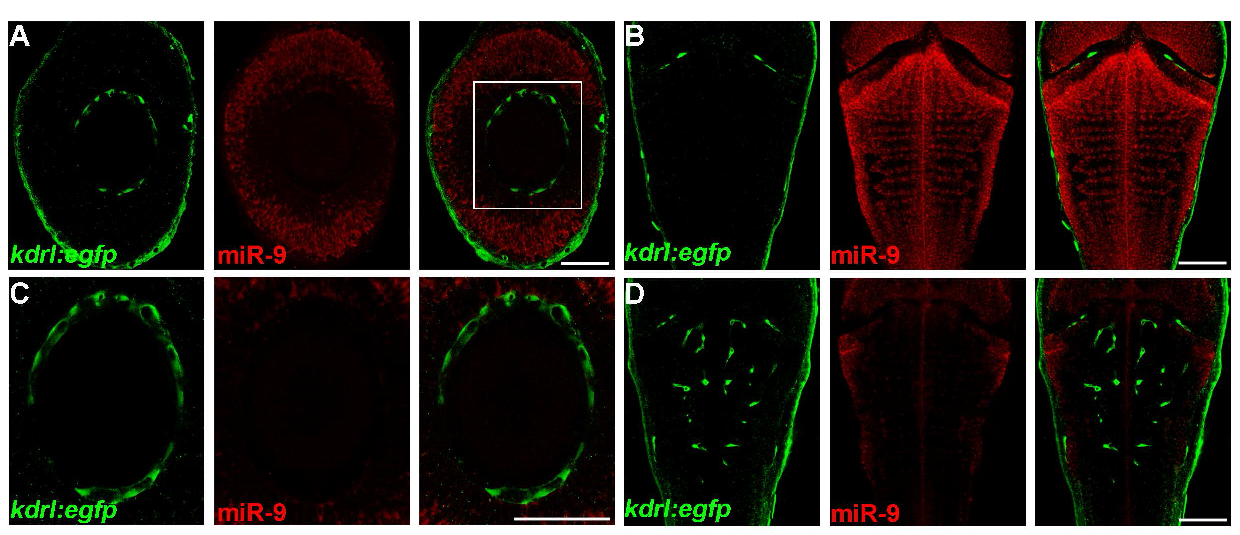
\epsfig{file=figures/zfishSnpsFigureS2.pdf,width=0.8
\linewidth,clip=,trim=0 0 0 0} \\
\end{tabular}
\caption[\emph{miR-9} expression is not detected in endothelial cells or blood vessels]{
{\bf \emph{miR-9} expression is not detected in endothelial cells or blood vessels.}
{\bf (A-D)} Confocal sections of double \emph{in
situ}/immunolabelling in \emph{Tg(kdrl:egfp)} embryos at 48 hpf showing
the absence of co-localization in the expression of the endogenous
\emph{miR-9} and EGFP protein in the retina and the hindbrain. Blood
vessels or endothelial cells are not localized in domains expressing
\emph{miR-9} in the retina {\bf (A)} and hindbrain {\bf (B)}. \emph{miR-9}
expression in not detected in \emph{kdrl:egfp+} cells in the retina {\bf (C)}
and hindbrain {\bf (D)}. Dorsal view of the brain with anterior up. Lateral
view of the retina. Scale bars: 100 $\mu$m.
}
\label{fig:zfishSnpsFigS2}
\end{figure}

\begin{landscape}
\begin{center}
\begin{longtable}{@{}>{\hspace{0pt}}p{0.1\linewidth}>{\hspace{0pt}}p{0.1\linewidth}>{\hspace{0pt}}p{0.2\linewidth}>{\hspace{0pt}}p{0.2\linewidth}>{\hspace{0pt}}p{0.06\linewidth}>{\hspace{0pt}}p{0.06\linewidth}>{\hspace{0pt}}p{0.2\linewidth}@{}}
\caption[Deeply conserved GWAS SNP screen results]{{\bf Deeply conserved GWAS SNP screen results.}
Sequence conservation blocks and gene synteny of GWAS
SNPs conserved between human and zebrafish.
}
\label{tab:zfishSnpsTabS1} \\

\hline \textbf{Variant rsIDs} & \textbf{Trait or disease} & \textbf{Human
coordinates} & \textbf{Zebrafish coordinates} & \textbf{nhmmer e-value}
& \textbf{nhmmer bit score} & \textbf{Syntenic genes (distance to
nearest transcript TSS)} \\ \hline 
\endfirsthead

\hline \textbf{Variant rsIDs} & \textbf{Trait or disease} & \textbf{Human
coordinates} & \textbf{Zebrafish coordinates} & \textbf{nhmmer e-value}
& \textbf{nhmmer bit score} & \textbf{Syntenic genes (distance to
nearest transcript TSS)} \\ \hline 
\endhead

\hline
\endlastfoot

rs6774494 & Nasopharyngeal carcinoma & hg19 chr3:169082534-169082733(+)
& danRer7 chr15:34810310-34810561(+) & 2.1E-39 & 142.6 &
MECOM(-95607): mecom(-136097)\tabularnewline
rs11190870 & Scoliosis & hg19 chr10:102979145-102979305(+) &
danRer7 chr13:28525660-28525820(+) & 2E-33 & 124.1 &
LBX1(+10326): lbx1a(+6000), TLX1(+85154): tlx1(-29839),
FBXW4(+393685): fbxw4(-210725)\tabularnewline
rs4759042 & Migraine & hg19 chr12:57377273-57377444(+) &
danRer7 chr9:49734712-49734883(+) & 3.3E-33 & 124.1 &
RDH16(-24200): dhrs9(+48910), SDR9C7(-49169): dhrs9(+48910),
HSD17B6(+197645): dhrs9(+48910)\tabularnewline
rs2307121 & Corneal structure & hg19 chr5:64625414-64625612(+) &
danRer7 chr10:11654536-11654735(+) & 1.3E-02 & 112.3 &
ADAMTS6(-66749): adamts6(+73188), PPWD1(-233550): ppwd1(-79052),
TRIM23(+281188): trim23(+151614),
CWC27(+445530): cwc27(+290628)\tabularnewline
rs17421627 & Retinal vascular caliber & hg19 chr5:87847488-87847679(+) &
danRer7 chr5:49928050-49928256(+) & 3.4E-25 & 97.8 &
MIR-9-5(+60011): mir-9-5(+24822), MEF2C(+177753): mef2cb(+114783),
TMEM161B(-282290): tmem161b(-74583)\tabularnewline
rs4880487 & Migraine & hg19 chr10:1246802-1246972(+) &
danRer7 chr24:3632273-3632449(+) & 8.6E-21 & 83.6 &
ADARB2(-562): adarb2(+228617), WDR37(+77140): wdr37(+69279),
IDI1(-151777): idi1(-77538), IDI2(-175088): idi1(-77538)\tabularnewline
rs16932455 & Capecitabine sensitivity & hg19 chr11:16040076-16040273(+)
& danRer7 chr7:28559360-28559558(-) & 1.1E-18 & 77.4 &
SOX6(-3301): sox6(-11158)\tabularnewline
rs13382811 & Myopia (severe) & hg19 chr2:145223523-145223713(+) &
danRer7 chr6:1000361-1000506(+) & 5.7E-18 & 74.6 &
ZEB2(-35481): zeb2b(-43451)\tabularnewline
rs17178006 & Hippocampal volume & hg19 chr12:65718213-65718383(+) &
danRer7 chr4:11967906-11968083(-) & 6.8E-18 & 73.7 &
MSRB3(-2357): msrb3(+5901), LEMD3(+78968): lemd3(+26539),
WIF1(-202952): wif1(-28293), HMGA2(-499613): hmga2(-41383)\tabularnewline
rs6588480 & Response to statin therapy & hg19 chr1:53978072-53978217(+)
& danRer7 chr8:18692520-18692665(-) & 5.4E-16 & 67.7 &
GLIS1(+221733): glis1b(+71584)\tabularnewline
rs12593813 & Restless legs syndrome & hg19 chr15:68036768-68036950(+) &
danRer7 chr18:19721646-19721823(+) & 9.6E-14 & 60.9 &
SKOR1(-75183): skor1b(-33588), C15orf61(+222736): C18H15orf61(+58092),
IQCH(+254506): iqch(+98454), PIAS1(-309658): pias1b(-49392),
AAGAB(-489326): aagab(-121211)\tabularnewline
rs12431307 & Obesity-related traits & hg19 chr13:80644586-80644716(+) &
danRer7 chr1:4209100-4209234(-) & 4.6E-12 & 55.2 &
SPRY2(+269143): spry2(+38248)\tabularnewline
rs4333130 & Ankylosing spondylitis & hg19 chr4:80949732-80949918(+) &
danRer7 chr5:41045298-41045471(+) & 1.2E-11 & 54.2 &
ANTXR2(+42949): antxr2a(+34553), PRDM8(-155208): prdm8b(-64707),
FGF5(-237928): fgf5(-97766),
C4orf22(-307049): C5H4orf22(-123872)\tabularnewline
rs2272046 & Polycystic ovary syndrome & hg19 chr12:66224444-66224542(+)
& danRer7 chr4:11918185-11918283(-) & 4.4E-11 & 51.5 &
HMGA2(+2712): hmga2(+8271), TMBIM4(+308224): tmbim4(+121765),
IRAK3(-358166): irak3(-62739), HELB(-471832): helb(-72528),
MSRB3(+486579): msrb3(+55661)\tabularnewline
rs2842643 & Attention deficit hyperactivity disorder &
hg19 chr6:41650647-41650827(+) & danRer7 chr11:23106736-23106903(+) &
8.8E-06 & 35.2 & TFEB(+5201): tfeb(+38515), MDFI(+36745): MDFI(+162564),
FOXP4(+112825): foxp4(+310951)\tabularnewline
rs2153271 & Freckling & hg19 chr9:16864430-16864610(+) &
danRer7 chr1:25994830-25994996(-) & 1.0E-04 & 30.9 &
BNC2(+6184): bnc2(+4776), CNTLN(-270460): cntln(-13956)\tabularnewline
rs7349332 & Hair morphology & hg19 chr2:219756333-219756404(+) &
danRer7 chr9:11675370-11675444(+) & 1.6E-03 & 26.7 &
WNT10A(-1575): wnt10a(+19316), WNT6(+31680): wnt6b(+105345),
CDK5R2(-68009): cdk5r2b(-132850), FEV(+92829): fev(+151222),
CRYBA2(+99561): cryba2b(+160934),
MIR375(+110063): dre-mir-375-2(+172880)\tabularnewline
rs7246657 & Coronary artery calcification &
hg19 chr19:37747060-37747144(+) & danRer7 chr3:8862134-8862229(+) &
1.6E-02 & 24.1 & ZNF850(483332): zgc:174234(234552)\tabularnewline
rs13414205 & Immune reponse to smallpox (secreted TNF-alpha) &
hg19 chr2:44662376-44662487(+) & danRer7 chr13:10168027-10168141(-) &
2.6E-02 & 23.7 & CAMKMT(+62544): CAMKMT(1of2)(+17764),
CAMKMT(+62544): camkmt(-171412), PREPL(-73430): prepl(-18369),
SLC3A1(+131486): slc3a1(+69409), PPM1B(+217470): ppm1ba(+124662),
LRPPRC(-439287): lrpprc(-196554)\tabularnewline
rs13095226 & Age-related macular degeneration &
hg19 chr3:99396188-99396298(+) & danRer7 chr22:29659198-29659297(-) &
1.2E-01 & 21.6 & COL8A1(-29672): col8a1b(-267444)\tabularnewline
rs1568679 & Response to antipsychotic treatment &
hg19 chr15:37349784-37349819(+) & danRer7 chr17:53456843-53456878(-) &
1.2E-01 & 21.3 & MEIS2(+36429): MEIS2(3of3)(+109701),
MEIS2(+36429): meis2a(+23451),
C15orf41(+301655): C17H15orf41(+16903)\tabularnewline
rs564148 & Response to amphetamines & hg19 chr1:34173731-34173831(+) &
danRer7 chr23:22192192-22192293(+) & 3.2E-01 & 20.1 &
PHC2(277077): phc2a(165332)\tabularnewline

\end{longtable}
\end{center}
\end{landscape}


    % Bibliography
    \bibliographystyle{modPlain}
    \bibliography{jnotwellThesis}

% Only include this if using the [online] specification with the suthesis-2e package
% If so, include this to be able to print out a copy of the signature page (on acid-free paper!)
% Still, comment it out in the copy of the dissertation you submit, since the signed copy will be
% digitally appended to your document.
%
%\onlinesignature

\end{document}

